% Options for packages loaded elsewhere
\PassOptionsToPackage{unicode}{hyperref}
\PassOptionsToPackage{hyphens}{url}
%
\documentclass[
]{book}
\usepackage{amsmath,amssymb}
\usepackage{iftex}
\ifPDFTeX
  \usepackage[T1]{fontenc}
  \usepackage[utf8]{inputenc}
  \usepackage{textcomp} % provide euro and other symbols
\else % if luatex or xetex
  \usepackage{unicode-math} % this also loads fontspec
  \defaultfontfeatures{Scale=MatchLowercase}
  \defaultfontfeatures[\rmfamily]{Ligatures=TeX,Scale=1}
\fi
\usepackage{lmodern}
\ifPDFTeX\else
  % xetex/luatex font selection
\fi
% Use upquote if available, for straight quotes in verbatim environments
\IfFileExists{upquote.sty}{\usepackage{upquote}}{}
\IfFileExists{microtype.sty}{% use microtype if available
  \usepackage[]{microtype}
  \UseMicrotypeSet[protrusion]{basicmath} % disable protrusion for tt fonts
}{}
\makeatletter
\@ifundefined{KOMAClassName}{% if non-KOMA class
  \IfFileExists{parskip.sty}{%
    \usepackage{parskip}
  }{% else
    \setlength{\parindent}{0pt}
    \setlength{\parskip}{6pt plus 2pt minus 1pt}}
}{% if KOMA class
  \KOMAoptions{parskip=half}}
\makeatother
\usepackage{xcolor}
\usepackage{color}
\usepackage{fancyvrb}
\newcommand{\VerbBar}{|}
\newcommand{\VERB}{\Verb[commandchars=\\\{\}]}
\DefineVerbatimEnvironment{Highlighting}{Verbatim}{commandchars=\\\{\}}
% Add ',fontsize=\small' for more characters per line
\usepackage{framed}
\definecolor{shadecolor}{RGB}{248,248,248}
\newenvironment{Shaded}{\begin{snugshade}}{\end{snugshade}}
\newcommand{\AlertTok}[1]{\textcolor[rgb]{0.94,0.16,0.16}{#1}}
\newcommand{\AnnotationTok}[1]{\textcolor[rgb]{0.56,0.35,0.01}{\textbf{\textit{#1}}}}
\newcommand{\AttributeTok}[1]{\textcolor[rgb]{0.13,0.29,0.53}{#1}}
\newcommand{\BaseNTok}[1]{\textcolor[rgb]{0.00,0.00,0.81}{#1}}
\newcommand{\BuiltInTok}[1]{#1}
\newcommand{\CharTok}[1]{\textcolor[rgb]{0.31,0.60,0.02}{#1}}
\newcommand{\CommentTok}[1]{\textcolor[rgb]{0.56,0.35,0.01}{\textit{#1}}}
\newcommand{\CommentVarTok}[1]{\textcolor[rgb]{0.56,0.35,0.01}{\textbf{\textit{#1}}}}
\newcommand{\ConstantTok}[1]{\textcolor[rgb]{0.56,0.35,0.01}{#1}}
\newcommand{\ControlFlowTok}[1]{\textcolor[rgb]{0.13,0.29,0.53}{\textbf{#1}}}
\newcommand{\DataTypeTok}[1]{\textcolor[rgb]{0.13,0.29,0.53}{#1}}
\newcommand{\DecValTok}[1]{\textcolor[rgb]{0.00,0.00,0.81}{#1}}
\newcommand{\DocumentationTok}[1]{\textcolor[rgb]{0.56,0.35,0.01}{\textbf{\textit{#1}}}}
\newcommand{\ErrorTok}[1]{\textcolor[rgb]{0.64,0.00,0.00}{\textbf{#1}}}
\newcommand{\ExtensionTok}[1]{#1}
\newcommand{\FloatTok}[1]{\textcolor[rgb]{0.00,0.00,0.81}{#1}}
\newcommand{\FunctionTok}[1]{\textcolor[rgb]{0.13,0.29,0.53}{\textbf{#1}}}
\newcommand{\ImportTok}[1]{#1}
\newcommand{\InformationTok}[1]{\textcolor[rgb]{0.56,0.35,0.01}{\textbf{\textit{#1}}}}
\newcommand{\KeywordTok}[1]{\textcolor[rgb]{0.13,0.29,0.53}{\textbf{#1}}}
\newcommand{\NormalTok}[1]{#1}
\newcommand{\OperatorTok}[1]{\textcolor[rgb]{0.81,0.36,0.00}{\textbf{#1}}}
\newcommand{\OtherTok}[1]{\textcolor[rgb]{0.56,0.35,0.01}{#1}}
\newcommand{\PreprocessorTok}[1]{\textcolor[rgb]{0.56,0.35,0.01}{\textit{#1}}}
\newcommand{\RegionMarkerTok}[1]{#1}
\newcommand{\SpecialCharTok}[1]{\textcolor[rgb]{0.81,0.36,0.00}{\textbf{#1}}}
\newcommand{\SpecialStringTok}[1]{\textcolor[rgb]{0.31,0.60,0.02}{#1}}
\newcommand{\StringTok}[1]{\textcolor[rgb]{0.31,0.60,0.02}{#1}}
\newcommand{\VariableTok}[1]{\textcolor[rgb]{0.00,0.00,0.00}{#1}}
\newcommand{\VerbatimStringTok}[1]{\textcolor[rgb]{0.31,0.60,0.02}{#1}}
\newcommand{\WarningTok}[1]{\textcolor[rgb]{0.56,0.35,0.01}{\textbf{\textit{#1}}}}
\usepackage{longtable,booktabs,array}
\usepackage{calc} % for calculating minipage widths
% Correct order of tables after \paragraph or \subparagraph
\usepackage{etoolbox}
\makeatletter
\patchcmd\longtable{\par}{\if@noskipsec\mbox{}\fi\par}{}{}
\makeatother
% Allow footnotes in longtable head/foot
\IfFileExists{footnotehyper.sty}{\usepackage{footnotehyper}}{\usepackage{footnote}}
\makesavenoteenv{longtable}
\usepackage{graphicx}
\makeatletter
\def\maxwidth{\ifdim\Gin@nat@width>\linewidth\linewidth\else\Gin@nat@width\fi}
\def\maxheight{\ifdim\Gin@nat@height>\textheight\textheight\else\Gin@nat@height\fi}
\makeatother
% Scale images if necessary, so that they will not overflow the page
% margins by default, and it is still possible to overwrite the defaults
% using explicit options in \includegraphics[width, height, ...]{}
\setkeys{Gin}{width=\maxwidth,height=\maxheight,keepaspectratio}
% Set default figure placement to htbp
\makeatletter
\def\fps@figure{htbp}
\makeatother
\setlength{\emergencystretch}{3em} % prevent overfull lines
\providecommand{\tightlist}{%
  \setlength{\itemsep}{0pt}\setlength{\parskip}{0pt}}
\setcounter{secnumdepth}{5}
\usepackage{booktabs}
\usepackage{amsthm}
\makeatletter
\def\thm@space@setup{%
  \thm@preskip=8pt plus 2pt minus 4pt
  \thm@postskip=\thm@preskip
}
\makeatother
\ifLuaTeX
  \usepackage{selnolig}  % disable illegal ligatures
\fi
\usepackage[]{natbib}
\bibliographystyle{apalike}
\IfFileExists{bookmark.sty}{\usepackage{bookmark}}{\usepackage{hyperref}}
\IfFileExists{xurl.sty}{\usepackage{xurl}}{} % add URL line breaks if available
\urlstyle{same}
\hypersetup{
  pdftitle={STA504 E-Pack: Mathematical Statistics with Calc. Rev.},
  pdfauthor={Cheng Peng},
  hidelinks,
  pdfcreator={LaTeX via pandoc}}

\title{STA504 E-Pack: Mathematical Statistics with Calc. Rev.}
\author{Cheng Peng}
\date{West Chester University}

\begin{document}
\maketitle

{
\setcounter{tocdepth}{1}
\tableofcontents
}
\begin{Shaded}
\begin{Highlighting}[]
\FunctionTok{install.packages}\NormalTok{(}\StringTok{"bookdown"}\NormalTok{)}
\CommentTok{\# or the development version}
\CommentTok{\# devtools::install\_github("rstudio/bookdown")}
\end{Highlighting}
\end{Shaded}

\hypertarget{introduction}{%
\chapter{Introduction}\label{introduction}}

This \emph{E-coursepack} is a self-contained homegrown Ebook that contains all topics covered in current STA504 at WCU.

All technical terms used in this Ebook are consistent with those used in the \emph{required} textbook. Students are not required to buy the Ebook from a publisher.

\hypertarget{use-of-technologies}{%
\section{Use of Technologies}\label{use-of-technologies}}

Although it is not required to use any software program in this class, you are still encouraged to use RMarkdown (for R users) or Jupyter Notebook (for Python users) to draft your assignments and practice basic graphical and computational capabilities of these software tools.

Both RMarkdown and Jupyter Notebook are very convenient to use in drafting technical documents that involves mathematical equations and graphics. To write mathematical formulas, you can use LaTex commands in Rmarkdown and Jupyter notebook.

\hypertarget{greek-letters}{%
\subsection{Greek Letters}\label{greek-letters}}

\begin{longtable}[]{@{}ll@{}}
\toprule\noalign{}
Symbol & Script \\
\midrule\noalign{}
\endhead
\bottomrule\noalign{}
\endlastfoot
\(\alpha\) & \texttt{\textbackslash{}alpha} \\
\(A\) & \texttt{A} \\
\(\beta\) & \texttt{\textbackslash{}beta} \\
\(B\) & \texttt{B} \\
\(\gamma\) & \texttt{\textbackslash{}gammma} \\
\(\Gamma\) & \texttt{\textbackslash{}Gamma} \\
\(\pi\) & \texttt{\textbackslash{}pi} \\
\(\Pi\) & \texttt{\textbackslash{}Pi} \\
\(\phi\) & \texttt{\textbackslash{}phi} \\
\(\Phi\) & \texttt{\textbackslash{}Phi} \\
\(\varphi\) & \texttt{\textbackslash{}varphi} \\
\(\theta\) & \texttt{\textbackslash{}theta} \\
\end{longtable}

\hypertarget{operators}{%
\subsection{Operators}\label{operators}}

\begin{longtable}[]{@{}ll@{}}
\toprule\noalign{}
Symbol & Script \\
\midrule\noalign{}
\endhead
\bottomrule\noalign{}
\endlastfoot
\(\cos\) & \texttt{\textbackslash{}cos} \\
\(\sin\) & \texttt{\textbackslash{}sin} \\
\(\lim\) & \texttt{\textbackslash{}lim} \\
\(\exp\) & \texttt{\textbackslash{}exp} \\
\(\to\) & \texttt{\textbackslash{}to} \\
\(\infty\) & \texttt{\textbackslash{}infty} \\
\(\equiv\) & \texttt{\textbackslash{}equiv} \\
\(\bmod\) & \texttt{\textbackslash{}bmod} \\
\(\times\) & \texttt{\textbackslash{}times} \\
\end{longtable}

\hypertarget{power-and-indicies}{%
\subsection{Power and Indicies}\label{power-and-indicies}}

\begin{longtable}[]{@{}ll@{}}
\toprule\noalign{}
Symbol & Script \\
\midrule\noalign{}
\endhead
\bottomrule\noalign{}
\endlastfoot
\(k_{n+1}\) & \texttt{k\_\{n+1\}} \\
\(n^2\) & \texttt{n\^{}2} \\
\(k_n^2\) & \texttt{k\_n\^{}2} \\
\end{longtable}

\hypertarget{fractions-and-binomials}{%
\subsection{Fractions and Binomials}\label{fractions-and-binomials}}

\begin{longtable}[]{@{}ll@{}}
\toprule\noalign{}
Symbol & Script \\
\midrule\noalign{}
\endhead
\bottomrule\noalign{}
\endlastfoot
\(\frac{n!}{k!(n-k)!}\) & \texttt{\textbackslash{}frac\{n!\}\{k!(n-k)!\}} \\
\(\binom{n}{k}\) & \texttt{\textbackslash{}binom\{n\}\{k\}} \\
\(\frac{\frac{x}{1}}{x - y}\) & \texttt{\textbackslash{}frac\{\textbackslash{}frac\{x\}\{1\}\}\{x\ -\ y\}} \\
\(^3/_7\) & \texttt{\^{}3/\_7} \\
\end{longtable}

\hypertarget{radical-roots}{%
\subsection{Radical Roots}\label{radical-roots}}

\begin{longtable}[]{@{}ll@{}}
\toprule\noalign{}
Symbol & Script \\
\midrule\noalign{}
\endhead
\bottomrule\noalign{}
\endlastfoot
\(\sqrt{k}\) & \texttt{\textbackslash{}sqrt\{k\}} \\
\(\sqrt[n]{k}\) & \texttt{\textbackslash{}sqrt{[}n{]}\{k\}} \\
\end{longtable}

\hypertarget{sums-integrals-and-related-symbols}{%
\subsection{Sums, Integrals, and Related Symbols}\label{sums-integrals-and-related-symbols}}

\begin{longtable}[]{@{}
  >{\raggedright\arraybackslash}p{(\columnwidth - 2\tabcolsep) * \real{0.4500}}
  >{\raggedright\arraybackslash}p{(\columnwidth - 2\tabcolsep) * \real{0.5500}}@{}}
\toprule\noalign{}
\begin{minipage}[b]{\linewidth}\raggedright
Symbol
\end{minipage} & \begin{minipage}[b]{\linewidth}\raggedright
Script
\end{minipage} \\
\midrule\noalign{}
\endhead
\bottomrule\noalign{}
\endlastfoot
\(\sum_{i=1}^{10} t_i\) & \texttt{\textbackslash{}sum\_\{i=1\}\^{}\{10\}\ t\_i} \\
\(\int_0^\infty \mathrm{e}^{-x},\mathrm{d}x\) & \texttt{\textbackslash{}int\_0\^{}\textbackslash{}infty\ \textbackslash{}mathrm\{e\}\^{}\{-x\},\textbackslash{}mathrm\{d\}x} \\
\(\sum\) & \texttt{\textbackslash{}sum} \\
\(\prod\) & \texttt{\textbackslash{}prod} \\
\(\coprod\) & \texttt{\textbackslash{}coprod} \\
\(\bigoplus\) & \texttt{\textbackslash{}bigoplus} \\
\(\bigotimes\) & \texttt{\textbackslash{}bigotimes} \\
\(\bigodot\) & \texttt{\textbackslash{}bigodot} \\
\(\bigcup\) & \texttt{\textbackslash{}bigcup} \\
\(\bigcap\) & \texttt{\textbackslash{}bigcap} \\
\(\biguplus\) & \texttt{\textbackslash{}biguplus} \\
\(\bigsqcup\) & \texttt{\textbackslash{}bigsqcup} \\
\(\bigvee\) & \texttt{\textbackslash{}bigvee} \\
\(\bigwedge\) & \texttt{\textbackslash{}bigwedge} \\
\(\int\) & \texttt{\textbackslash{}int} \\
\(\oint\) & \texttt{\textbackslash{}oint} \\
\(\iint\) & \texttt{\textbackslash{}iint} \\
\(\iiint\) & \texttt{\textbackslash{}iiint} \\
\(\idotsint\) & \texttt{\textbackslash{}idotsint} \\
\(\sum_{\substack{0<i<m, \ 0<j<n}} P(i, j)\) & \texttt{\textbackslash{}sum\_\{\textbackslash{}substack\{0\textless{}i\textless{}m,\ \textbackslash{}\ 0\textless{}j\textless{}n\}\}\ P(i,\ j)} \\
\(\int\limits_a^b\) & \texttt{\textbackslash{}int\textbackslash{}limits\_a\^{}b} \\
\end{longtable}

\hypertarget{more-special-symbols}{%
\subsection{More Special Symbols}\label{more-special-symbols}}

\begin{longtable}[]{@{}ll@{}}
\toprule\noalign{}
Symbol & Script \\
\midrule\noalign{}
\endhead
\bottomrule\noalign{}
\endlastfoot
\(a^{\prime}\) & \texttt{a\^{}\{\textbackslash{}prime\}} \\
\(a^{\prime\prime}\) & \texttt{a\^{}\{\textbackslash{}prime\textbackslash{}prime\}} \\
\(\hat{a}\) & \texttt{\textbackslash{}hat\{a\}} \\
\(\bar{a}\) & \texttt{\textbackslash{}bar\{a\}} \\
\(\grave{a}\) & \texttt{\textbackslash{}grave\{a\}} \\
\(\acute{a}\) & \texttt{\textbackslash{}acute\{a\}} \\
\(\dot{a}\) & \texttt{\textbackslash{}dot\{a\}} \\
\(\ddot{a}\) & \texttt{\textbackslash{}ddot\{a\}} \\
\(\not{a}\) & \texttt{\textbackslash{}not\{a\}} \\
\(\mathring{a}\) & \texttt{\textbackslash{}mathring\{a\}} \\
\(\overrightarrow{AB}\) & \texttt{\textbackslash{}overrightarrow\{AB\}} \\
\(\overleftarrow{AB}\) & \texttt{\textbackslash{}overleftarrow\{AB\}} \\
\(a^{\prime\prime\prime}\) & \texttt{a\^{}\{\textbackslash{}prime\textbackslash{}prime\textbackslash{}prime\}} \\
\(\overline{aaa}\) & \texttt{\textbackslash{}overline\{aaa\}} \\
\(\check{a}\) & \texttt{\textbackslash{}check\{a\}} \\
\(\vec{a}\) & \texttt{\textbackslash{}vec\{a\}} \\
\(\underline{a}\) & \texttt{\textbackslash{}underline\{a\}} \\
\(\color{red}x\) & \texttt{\textbackslash{}color\{red\}x} \\
\(\pm\) & \texttt{\textbackslash{}pm} \\
\(\mp\) & \texttt{\textbackslash{}mp} \\
\(\int y \mathrm{d}x\) & \texttt{\textbackslash{}int\ y\ \textbackslash{}mathrm\{d\}x} \\
\(,\) & \texttt{,} \\
\(:\) & \texttt{:} \\
\(;\) & \texttt{;} \\
\(!\) & \texttt{!} \\
\(\int y, \mathrm{d}x\) & \texttt{\textbackslash{}int\ y,\ \textbackslash{}mathrm\{d\}x} \\
\(\dots\) & \texttt{\textbackslash{}dots} \\
\(\ldots\) & \texttt{\textbackslash{}ldots} \\
\(\cdots\) & \texttt{\textbackslash{}cdots} \\
\(\vdots\) & \texttt{\textbackslash{}vdots} \\
\(\ddots\) & \texttt{\textbackslash{}ddots} \\
\end{longtable}

\hypertarget{brackets}{%
\subsection{Brackets}\label{brackets}}

\begin{longtable}[]{@{}ll@{}}
\toprule\noalign{}
Symbol & Script \\
\midrule\noalign{}
\endhead
\bottomrule\noalign{}
\endlastfoot
\((a)\) & \texttt{(a)} \\
\([a]\) & \texttt{{[}a{]}} \\
\(\{a\}\) & \texttt{\textbackslash{}\{a\textbackslash{}\}} \\
\(\langle f \rangle\) & \texttt{\textbackslash{}langle\ f\ \textbackslash{}rangle} \\
\(\lfloor f \rfloor\) & \texttt{\textbackslash{}lfloor\ f\ \textbackslash{}rfloor} \\
\(\lceil f \rceil\) & \texttt{\textbackslash{}lceil\ f\ \textbackslash{}rceil} \\
\(\ulcorner f \urcorner\) & \texttt{\textbackslash{}ulcorner\ f\ \textbackslash{}urcorner} \\
\end{longtable}

\hypertarget{matrix}{%
\subsection{Matrix}\label{matrix}}

\begin{verbatim}
$$
X_{m,n} = 
\begin{pmatrix}
  x_{1,1} & x_{1,2} & \cdots & x_{1,n} \\
  x_{2,1} & x_{2,2} & \cdots & x_{2,n} \\
  \vdots  & \vdots  & \ddots & \vdots  \\
  x_{m,1} & x_{m,2} & \cdots & x_{m,n} 
\end{pmatrix}
$$
\end{verbatim}

produces

\[
X_{m,n} = 
\begin{pmatrix}
  x_{1,1} & x_{1,2} & \cdots & x_{1,n} \\
  x_{2,1} & x_{2,2} & \cdots & x_{2,n} \\
  \vdots  & \vdots  & \ddots & \vdots  \\
  x_{m,1} & x_{m,2} & \cdots & x_{m,n} 
\end{pmatrix}
\]

\begin{verbatim}
$$
M = 
\begin{bmatrix}
\frac{5}{6} & \frac{1}{6} & 0 \\[0.3em]
\frac{5}{6} & 0 & \frac{1}{6} \\[0.3em]
0 & \frac{5}{6} & \frac{1}{6}
\end{bmatrix}
$$
\end{verbatim}

produces

\[
M = 
\begin{bmatrix}
\frac{5}{6} & \frac{1}{6} & 0 \\[0.3em]
\frac{5}{6} & 0 & \frac{1}{6} \\[0.3em]
0 & \frac{5}{6} & \frac{1}{6}
\end{bmatrix}
\]

\hypertarget{aligned-equations}{%
\subsection{Aligned Equations}\label{aligned-equations}}

\begin{verbatim}
$$
\begin{aligned}
Bias(\hat{\theta})  &= E(\hat{\theta}) - \theta \\
Bias(\hat{\theta})  &= E(2 \bar{X} -1) - \theta \\
Bias(\hat{\theta})  &= \frac{2}{n}\sum_{i=1}^n E(X_i) -1 -\theta \\
Bias(\hat{\theta})  &= 2E(X) - 1 - \theta \\
Bias(\hat{\theta})  &= 2 \cdot \frac{\theta+1}{2} - 1 - \theta \\
Bias(\hat{\theta})  &= 0 \\
\end{aligned}
$$
\end{verbatim}

Produces the following system of equations

\[
\begin{aligned}
Bias(\hat{\theta})  &= E(\hat{\theta}) - \theta \\
Bias(\hat{\theta})  &= E(2 \bar{X} -1) - \theta \\
Bias(\hat{\theta})  &= \frac{2}{n}\sum_{i=1}^n E(X_i) -1 -\theta \\
Bias(\hat{\theta})  &= 2E(X) - 1 - \theta \\
Bias(\hat{\theta})  &= 2 \cdot \frac{\theta+1}{2} - 1 - \theta \\
Bias(\hat{\theta})  &= 0 \\
\end{aligned}
\]

\hypertarget{piece-wise-function}{%
\subsection{Piece-wise Function}\label{piece-wise-function}}

\begin{verbatim}
$$ f(x) = \begin{cases} \frac{1}{b-a} \\ 0 \end{cases} $$
\end{verbatim}

produces the following piece-wise function

\[ f(x) = \begin{cases} \frac{1}{b-a} \\ 0 \end{cases} \]

\hypertarget{including-images-and-graphics}{%
\section{Including Images and Graphics}\label{including-images-and-graphics}}

One can write code in either R (in RMarkdown code chunk) or Python (in Jupyter notebook cell) to produce graphics such as density curves or distribution histograms for different random variables. Sometimes, one can also include external (dynamic or static) images in the document.

Since both RMarkdown and Jupyter notebook support HTML syntax, we can use HTML image tag to include external images into the documet. In the mean while they also support LaTex () style commands, wecould also use LaTex command to include images to the document.

\hypertarget{r-plot-function}{%
\section{R plot() Function}\label{r-plot-function}}

Every programming language has its base plot functions to make graphics. We use base R \texttt{plot()} function as an example to show how to use it and \textbf{related graphical functions} to make high quality graphics in R.

For illustration, we use the standard normal distribution as an example to demonstrate how to make a nice graph to display important information. The probability density function of the standard normal density has the following form

\[
\phi(z) = \frac{1}{\sqrt{2}}e^{-z^2/2}, \mbox{ where } -\infty < z <\infty.
\]

The x-coordinates to be used are: -3.0, -2.6, -2.2, -1.8, -1.4, -1.0, -0.6, -0.2, 0.2, 0.6, 1.0, 1.4, 1.8, 2.2, 2.6, 3.0. We can then use the above density function to calculate the corresponding y-coordinates. In R, we use the following code to define the coordinates of the above 16 points on the density curve.

\begin{Shaded}
\begin{Highlighting}[]
\NormalTok{x }\OtherTok{=} \FunctionTok{c}\NormalTok{(}\SpecialCharTok{{-}}\FloatTok{3.0}\NormalTok{,}\SpecialCharTok{{-}}\FloatTok{2.6}\NormalTok{,}\SpecialCharTok{{-}}\FloatTok{2.2}\NormalTok{,}\SpecialCharTok{{-}}\FloatTok{1.8}\NormalTok{,}\SpecialCharTok{{-}}\FloatTok{1.4}\NormalTok{,}\SpecialCharTok{{-}}\FloatTok{1.0}\NormalTok{,}\SpecialCharTok{{-}}\FloatTok{0.6}\NormalTok{,}\SpecialCharTok{{-}}\FloatTok{0.2}\NormalTok{,}\DecValTok{0}\NormalTok{, }\FloatTok{0.2}\NormalTok{,}\FloatTok{0.6}\NormalTok{,}\FloatTok{1.0}\NormalTok{,}\FloatTok{1.4}\NormalTok{,}\FloatTok{1.8}\NormalTok{, }\FloatTok{2.2}\NormalTok{,}\FloatTok{2.6}\NormalTok{,}\FloatTok{3.0}\NormalTok{)}
\NormalTok{y }\OtherTok{=}\NormalTok{ (}\DecValTok{1}\SpecialCharTok{/}\FunctionTok{sqrt}\NormalTok{(}\DecValTok{2}\NormalTok{))}\SpecialCharTok{*}\FunctionTok{exp}\NormalTok{(}\SpecialCharTok{{-}}\NormalTok{x}\SpecialCharTok{\^{}}\DecValTok{2}\SpecialCharTok{/}\DecValTok{2}\NormalTok{)}
\end{Highlighting}
\end{Shaded}

\hypertarget{the-plot-function}{%
\subsection{\texorpdfstring{The \texttt{plot()} function}{The plot() function}}\label{the-plot-function}}

In R, the base graphics function to create a plot is the plot() function. It has many options and arguments to control many things, such as the plot type, labels, titles and colors. The plotting process is analogous to the hand drawing process: make a base plot and then add additional graphical components to make the graph more informative, understandable, and aesthetically pleasant.

The syntax of \texttt{plot()} is

\begin{verbatim}
plot(x,y,type,main,xlab,ylab,pch,col,las,bty,bg,cex,…)
\end{verbatim}

where the graphical arguments(parameters) are given by

\begin{figure}

{\centering 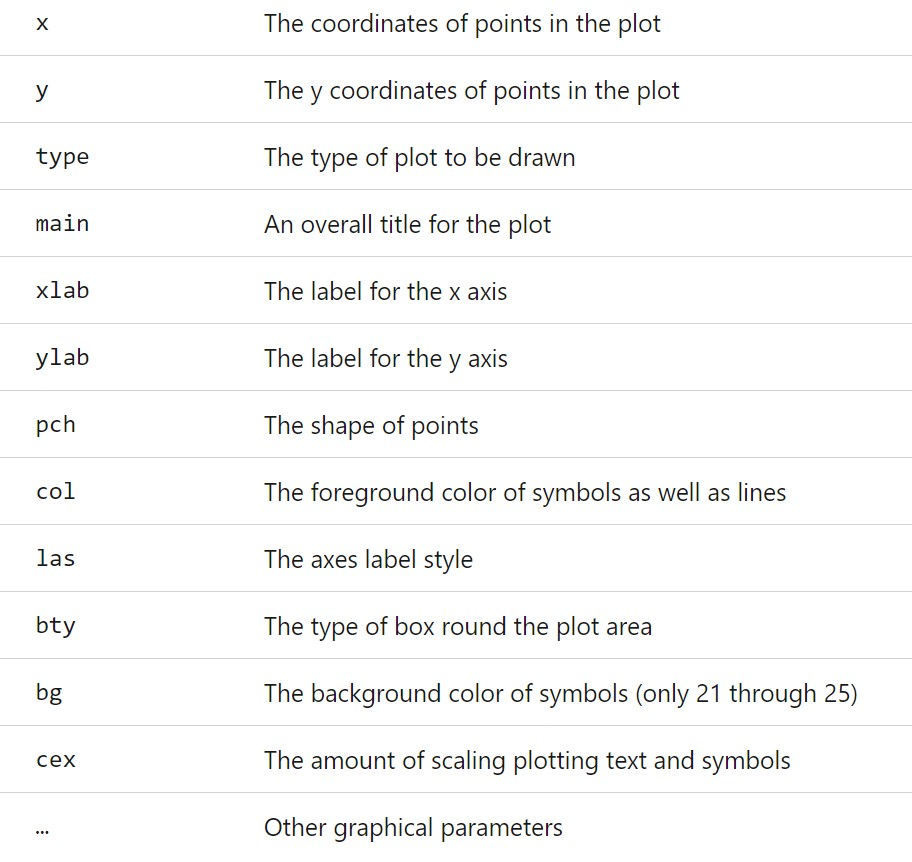
\includegraphics[width=0.7\linewidth]{img01/w01-plotArguments} 

}

\caption{plot() arguments}\label{fig:unnamed-chunk-4}
\end{figure}

The two coordinates must be paired (represent the location of the corresponding point), \texttt{main} is a string representing the name of the plot. \texttt{xlab} and \texttt{ylab} are also strings reflecting the labels of x- and y-axes.

The rest of the listed arguments have different choices. Next, we list the choices you can use to decorate your plot.

\hypertarget{type-plot-types}{%
\subsubsection{\texorpdfstring{\texttt{type}: Plot Types}{type: Plot Types}}\label{type-plot-types}}

The argument \texttt{type} is a string argument. Different string value representing different types.

\begin{figure}

{\centering 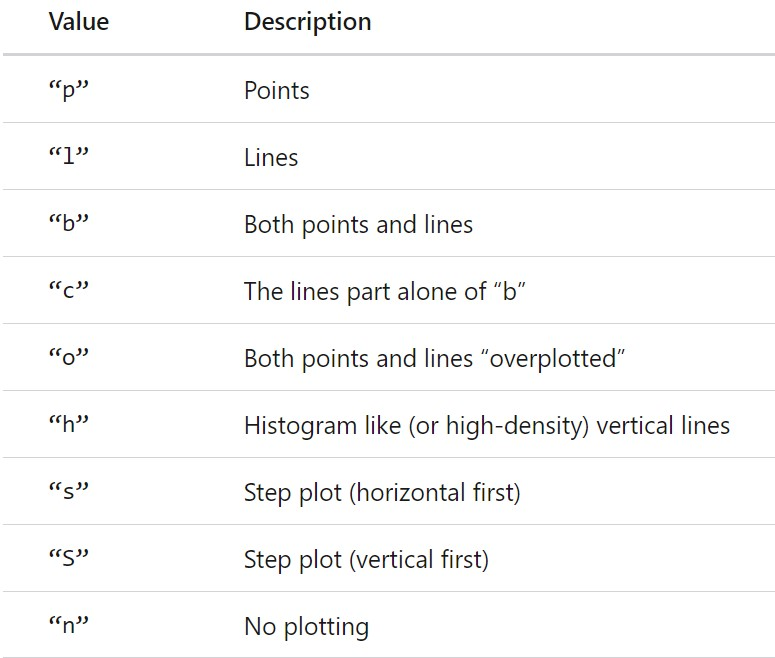
\includegraphics[width=0.7\linewidth]{img01/w01-plotType} 

}

\caption{Types of plot in R}\label{fig:unnamed-chunk-5}
\end{figure}

We plot the above normal density function in different types.

\begin{Shaded}
\begin{Highlighting}[]
\FunctionTok{par}\NormalTok{(}\AttributeTok{mfrow =} \FunctionTok{c}\NormalTok{(}\DecValTok{3}\NormalTok{,}\DecValTok{3}\NormalTok{), }\AttributeTok{mar=}\FunctionTok{c}\NormalTok{(}\DecValTok{2}\NormalTok{, }\DecValTok{2}\NormalTok{, }\DecValTok{4}\NormalTok{, }\FloatTok{0.5}\NormalTok{), }\AttributeTok{oma =} \FunctionTok{c}\NormalTok{(}\FloatTok{0.1}\NormalTok{, }\FloatTok{0.1}\NormalTok{, }\FloatTok{0.1}\NormalTok{, }\FloatTok{0.1}\NormalTok{))}
\FunctionTok{plot}\NormalTok{(x, y, }\AttributeTok{type =} \StringTok{"p"}\NormalTok{, }\AttributeTok{main =} \StringTok{"type=\textquotesingle{}p\textquotesingle{}"}\NormalTok{, }\AttributeTok{xlab =} \StringTok{""}\NormalTok{, }\AttributeTok{ylab=}\StringTok{""}\NormalTok{)}
\FunctionTok{plot}\NormalTok{(x, y, }\AttributeTok{type =} \StringTok{"l"}\NormalTok{, }\AttributeTok{main =} \StringTok{"type=\textquotesingle{}l\textquotesingle{}"}\NormalTok{, }\AttributeTok{xlab =} \StringTok{""}\NormalTok{, }\AttributeTok{ylab=}\StringTok{""}\NormalTok{)}
\FunctionTok{plot}\NormalTok{(x, y, }\AttributeTok{type =} \StringTok{"b"}\NormalTok{, }\AttributeTok{main =} \StringTok{"type=\textquotesingle{}b\textquotesingle{}"}\NormalTok{, }\AttributeTok{xlab =} \StringTok{""}\NormalTok{, }\AttributeTok{ylab=}\StringTok{""}\NormalTok{)}
\FunctionTok{plot}\NormalTok{(x, y, }\AttributeTok{type =} \StringTok{"c"}\NormalTok{, }\AttributeTok{main =} \StringTok{"type=\textquotesingle{}c\textquotesingle{}"}\NormalTok{, }\AttributeTok{xlab =} \StringTok{""}\NormalTok{, }\AttributeTok{ylab=}\StringTok{""}\NormalTok{)}
\FunctionTok{plot}\NormalTok{(x, y, }\AttributeTok{type =} \StringTok{"o"}\NormalTok{, }\AttributeTok{main =} \StringTok{"type=\textquotesingle{}o\textquotesingle{}"}\NormalTok{, }\AttributeTok{xlab =} \StringTok{""}\NormalTok{, }\AttributeTok{ylab=}\StringTok{""}\NormalTok{)}
\FunctionTok{plot}\NormalTok{(x, y, }\AttributeTok{type =} \StringTok{"h"}\NormalTok{, }\AttributeTok{main =} \StringTok{"type=\textquotesingle{}h\textquotesingle{}"}\NormalTok{, }\AttributeTok{xlab =} \StringTok{""}\NormalTok{, }\AttributeTok{ylab=}\StringTok{""}\NormalTok{)}
\FunctionTok{plot}\NormalTok{(x, y, }\AttributeTok{type =} \StringTok{"s"}\NormalTok{, }\AttributeTok{main =} \StringTok{"type=\textquotesingle{}s\textquotesingle{}"}\NormalTok{, }\AttributeTok{xlab =} \StringTok{""}\NormalTok{, }\AttributeTok{ylab=}\StringTok{""}\NormalTok{)}
\FunctionTok{plot}\NormalTok{(x, y, }\AttributeTok{type =} \StringTok{"S"}\NormalTok{, }\AttributeTok{main =} \StringTok{"type=\textquotesingle{}S\textquotesingle{}"}\NormalTok{, }\AttributeTok{xlab =} \StringTok{""}\NormalTok{, }\AttributeTok{ylab=}\StringTok{""}\NormalTok{)}
\FunctionTok{plot}\NormalTok{(x, y, }\AttributeTok{type =} \StringTok{"n"}\NormalTok{, }\AttributeTok{main =} \StringTok{"type=\textquotesingle{}n\textquotesingle{}"}\NormalTok{, }\AttributeTok{xlab =} \StringTok{""}\NormalTok{, }\AttributeTok{ylab=}\StringTok{""}\NormalTok{)}
\end{Highlighting}
\end{Shaded}

\begin{figure}

{\centering 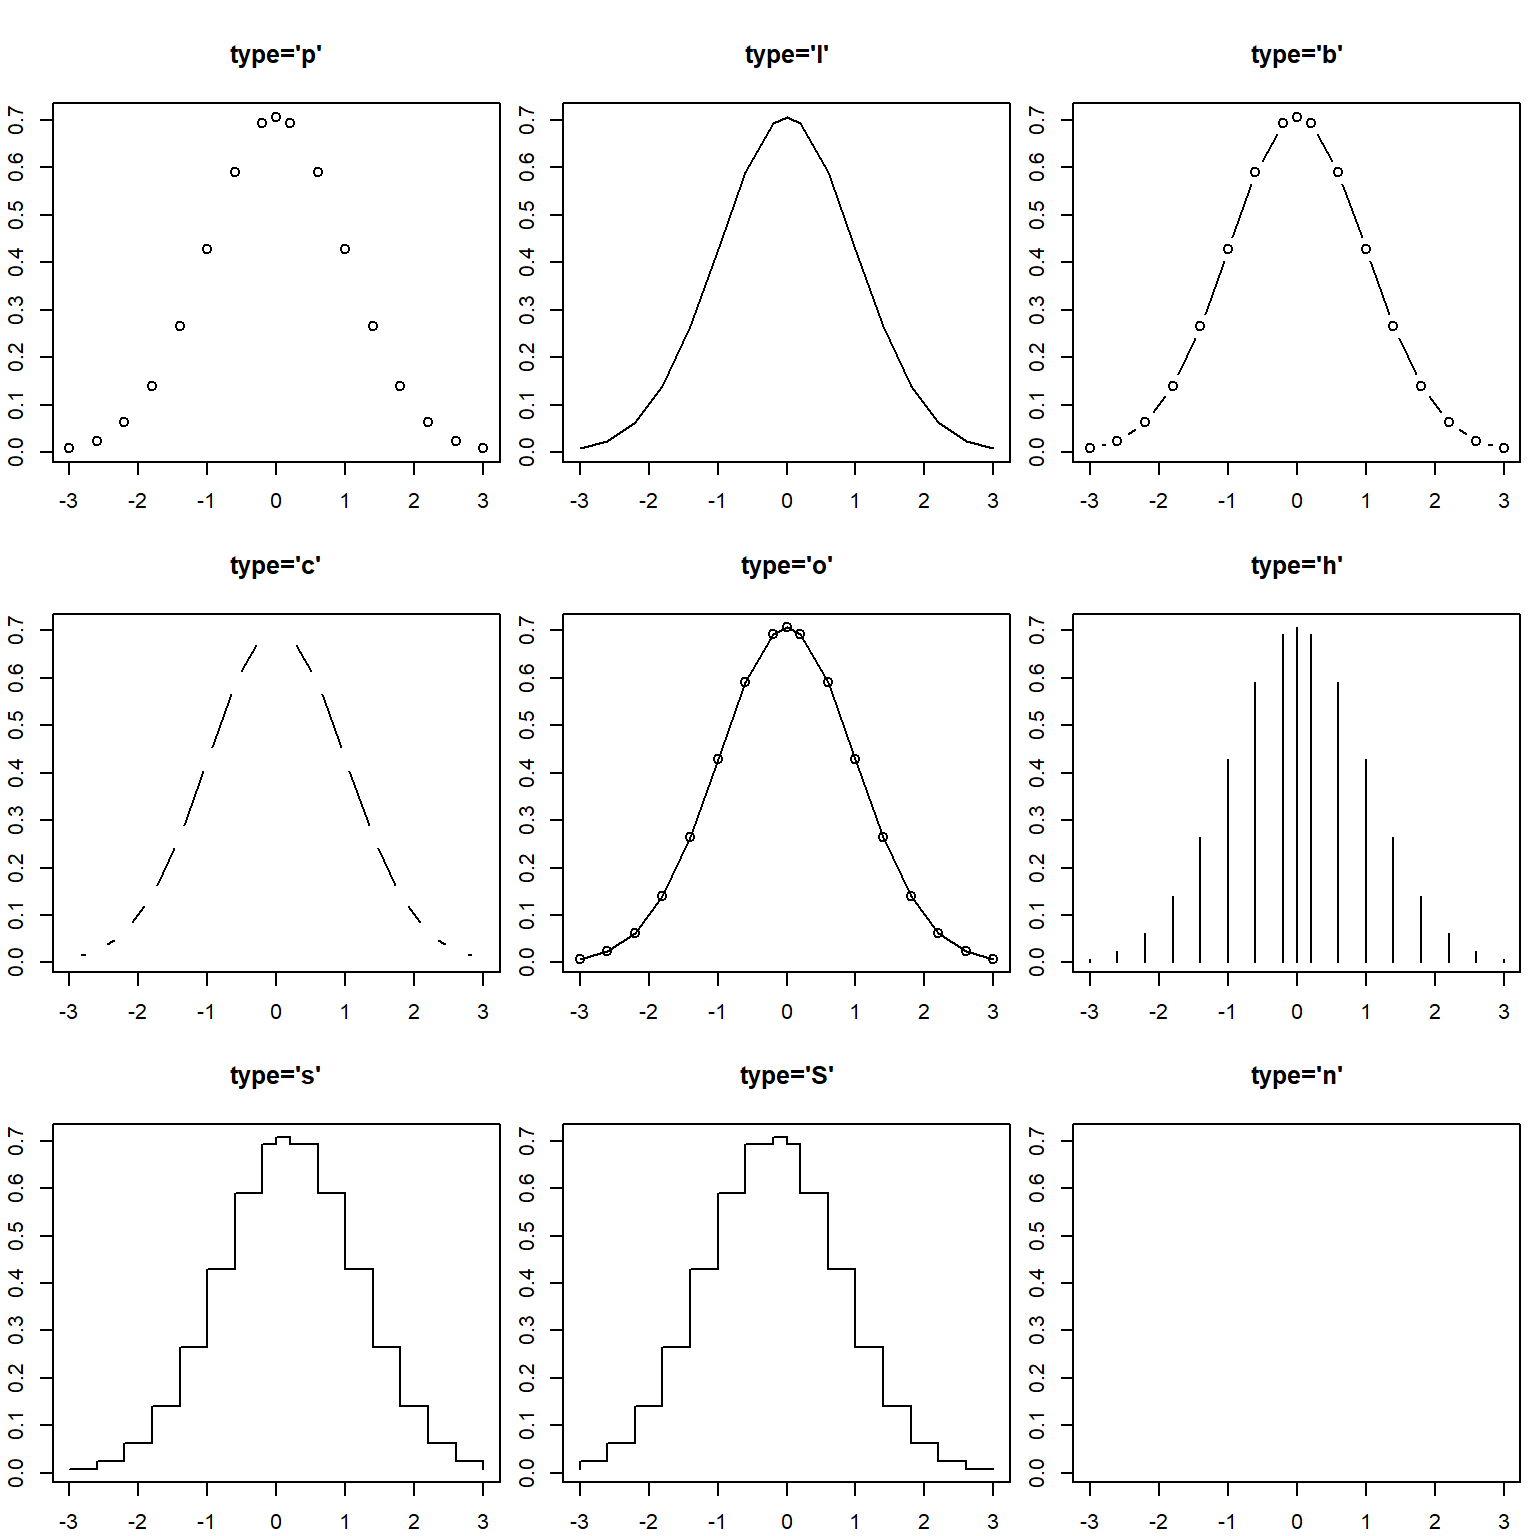
\includegraphics{STA504EB_files/figure-latex/unnamed-chunk-6-1} 

}

\caption{Different types of normal density function}\label{fig:unnamed-chunk-6}
\end{figure}

\hypertarget{pch-point-shapes}{%
\subsubsection{\texorpdfstring{\texttt{pch}: Point Shapes}{pch: Point Shapes}}\label{pch-point-shapes}}

The argument \texttt{pch} is point shape which takes a character value representing different shapes of the point you can choose for \texttt{plot()} function. Here is the table of possible point shape.

\begin{figure}

{\centering 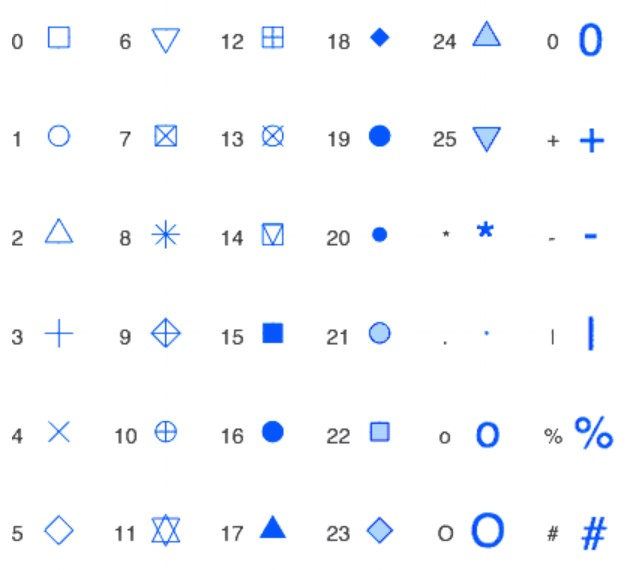
\includegraphics[width=0.6\linewidth]{img01/w01-PointShape} 

}

\caption{Point shapes in R}\label{fig:unnamed-chunk-7}
\end{figure}

In the following figure, we choose a few different shapes to demonstrate the ways of choosing different point shapes.

\begin{Shaded}
\begin{Highlighting}[]
\FunctionTok{par}\NormalTok{(}\AttributeTok{mfrow =} \FunctionTok{c}\NormalTok{(}\DecValTok{3}\NormalTok{,}\DecValTok{3}\NormalTok{), }\AttributeTok{mar=}\FunctionTok{c}\NormalTok{(}\DecValTok{2}\NormalTok{, }\DecValTok{2}\NormalTok{, }\DecValTok{4}\NormalTok{, }\FloatTok{0.5}\NormalTok{), }\AttributeTok{oma =} \FunctionTok{c}\NormalTok{(}\FloatTok{0.1}\NormalTok{, }\FloatTok{0.1}\NormalTok{, }\FloatTok{0.1}\NormalTok{, }\FloatTok{0.1}\NormalTok{))}
\FunctionTok{plot}\NormalTok{(x, y, }\AttributeTok{type =} \StringTok{"b"}\NormalTok{, }\AttributeTok{pch =} \DecValTok{1}\NormalTok{, }\AttributeTok{main =} \StringTok{"pch = 1"}\NormalTok{, }\AttributeTok{xlab =} \StringTok{""}\NormalTok{, }\AttributeTok{ylab=}\StringTok{""}\NormalTok{)}
\FunctionTok{plot}\NormalTok{(x, y, }\AttributeTok{type =} \StringTok{"b"}\NormalTok{, }\AttributeTok{pch =} \DecValTok{3}\NormalTok{, }\AttributeTok{main =} \StringTok{"pch = 3"}\NormalTok{, }\AttributeTok{xlab =} \StringTok{""}\NormalTok{, }\AttributeTok{ylab=}\StringTok{""}\NormalTok{)}
\FunctionTok{plot}\NormalTok{(x, y, }\AttributeTok{type =} \StringTok{"b"}\NormalTok{, }\AttributeTok{pch =} \DecValTok{5}\NormalTok{, }\AttributeTok{main =} \StringTok{"pch = 5"}\NormalTok{, }\AttributeTok{xlab =} \StringTok{""}\NormalTok{, }\AttributeTok{ylab=}\StringTok{""}\NormalTok{)}
\FunctionTok{plot}\NormalTok{(x, y, }\AttributeTok{type =} \StringTok{"b"}\NormalTok{, }\AttributeTok{pch =} \DecValTok{7}\NormalTok{, }\AttributeTok{main =} \StringTok{"pch = 7"}\NormalTok{, }\AttributeTok{xlab =} \StringTok{""}\NormalTok{, }\AttributeTok{ylab=}\StringTok{""}\NormalTok{)}
\FunctionTok{plot}\NormalTok{(x, y, }\AttributeTok{type =} \StringTok{"b"}\NormalTok{, }\AttributeTok{pch =} \DecValTok{9}\NormalTok{, }\AttributeTok{main =} \StringTok{"pch = 9"}\NormalTok{, }\AttributeTok{xlab =} \StringTok{""}\NormalTok{, }\AttributeTok{ylab=}\StringTok{""}\NormalTok{)}
\FunctionTok{plot}\NormalTok{(x, y, }\AttributeTok{type =} \StringTok{"b"}\NormalTok{, }\AttributeTok{pch =} \DecValTok{11}\NormalTok{, }\AttributeTok{main =} \StringTok{"pch = 11"}\NormalTok{, }\AttributeTok{xlab =} \StringTok{""}\NormalTok{, }\AttributeTok{ylab=}\StringTok{""}\NormalTok{)}
\FunctionTok{plot}\NormalTok{(x, y, }\AttributeTok{type =} \StringTok{"b"}\NormalTok{, }\AttributeTok{pch =} \DecValTok{13}\NormalTok{, }\AttributeTok{main =} \StringTok{"pch = 13"}\NormalTok{, }\AttributeTok{xlab =} \StringTok{""}\NormalTok{, }\AttributeTok{ylab=}\StringTok{""}\NormalTok{)}
\FunctionTok{plot}\NormalTok{(x, y, }\AttributeTok{type =} \StringTok{"b"}\NormalTok{, }\AttributeTok{pch =} \DecValTok{17}\NormalTok{, }\AttributeTok{main =} \StringTok{"pch = 17"}\NormalTok{, }\AttributeTok{xlab =} \StringTok{""}\NormalTok{, }\AttributeTok{ylab=}\StringTok{""}\NormalTok{)}
\FunctionTok{plot}\NormalTok{(x, y, }\AttributeTok{type =} \StringTok{"b"}\NormalTok{, }\AttributeTok{pch =} \DecValTok{21}\NormalTok{, }\AttributeTok{main =} \StringTok{"pch = 21"}\NormalTok{, }\AttributeTok{xlab =} \StringTok{""}\NormalTok{, }\AttributeTok{ylab=}\StringTok{""}\NormalTok{)}
\end{Highlighting}
\end{Shaded}

\begin{figure}

{\centering 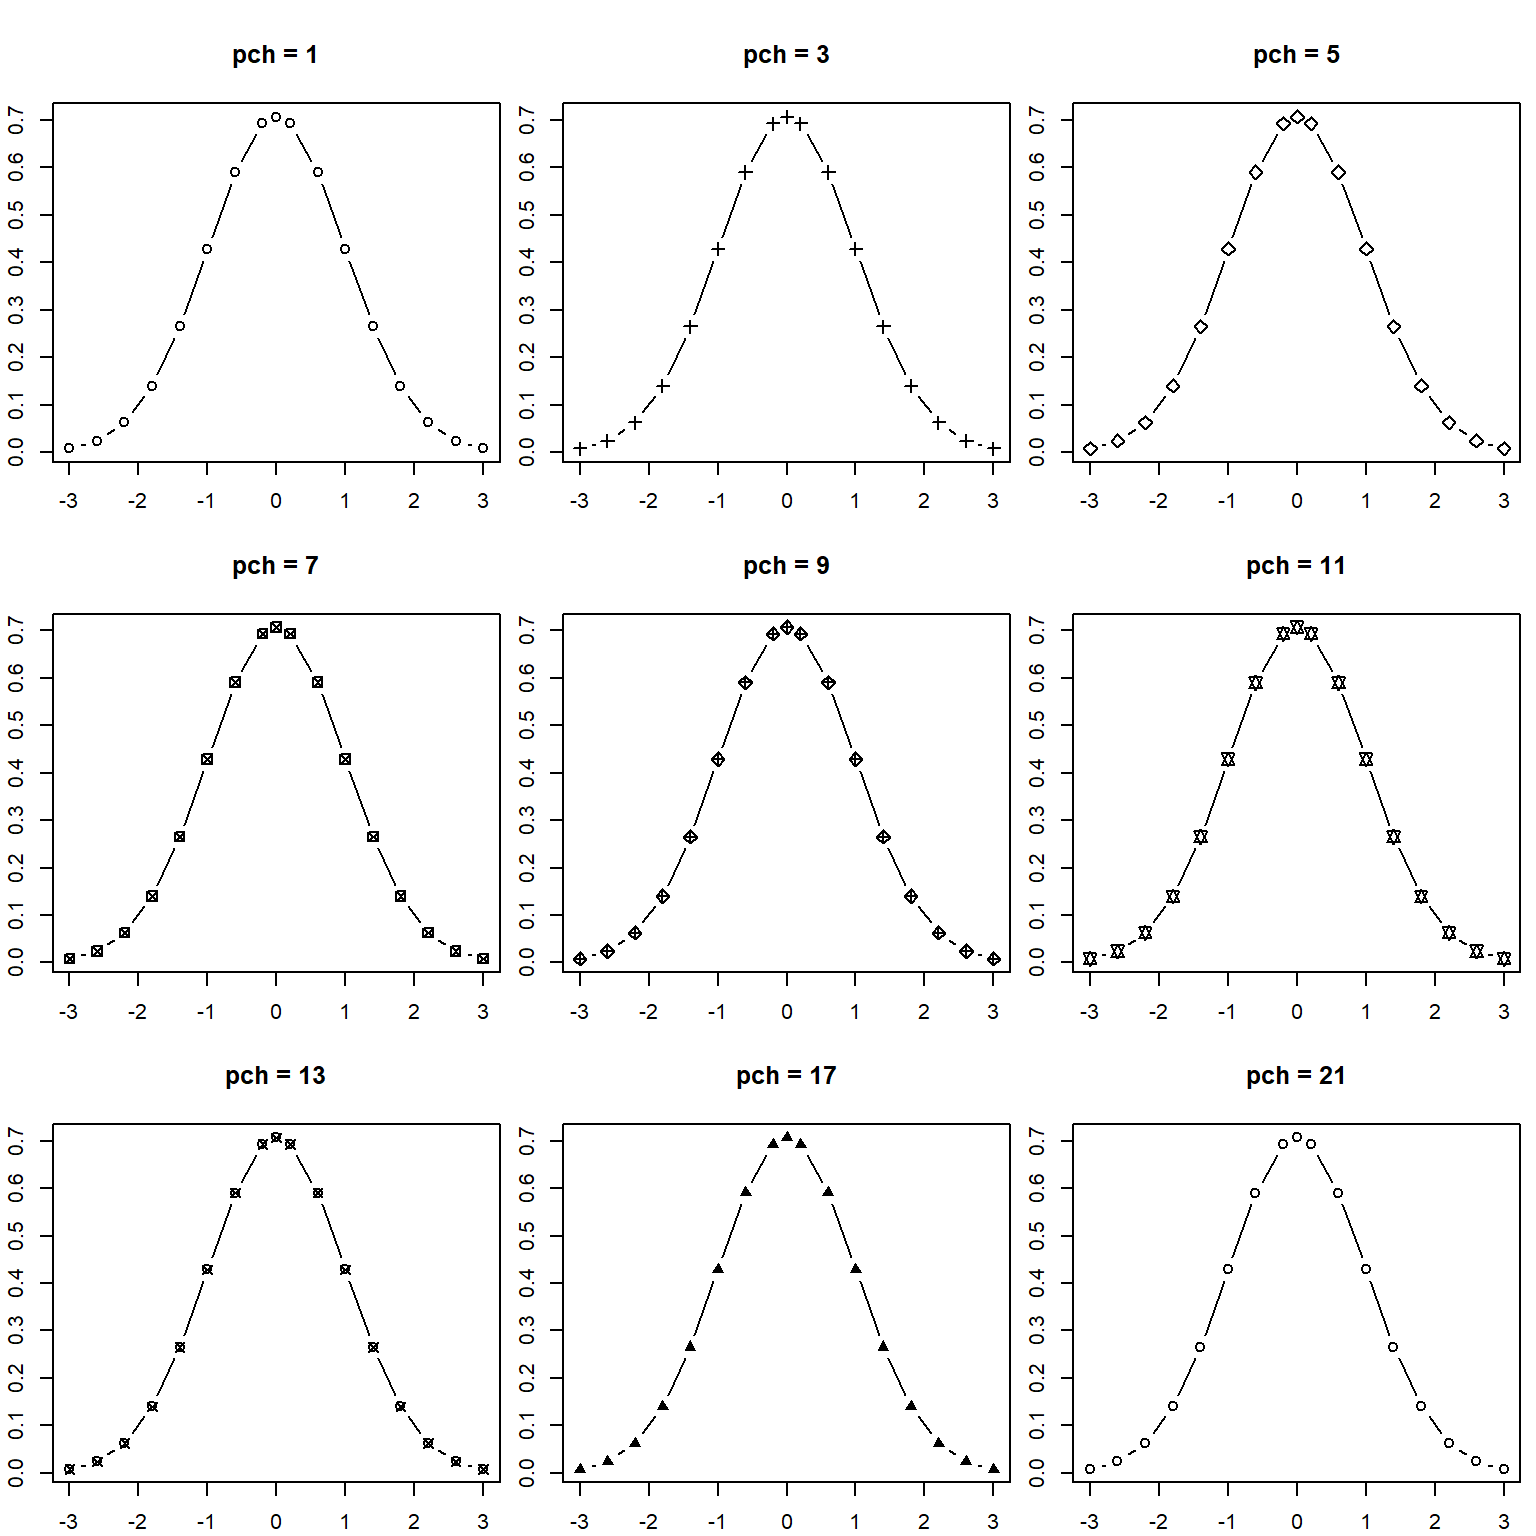
\includegraphics{STA504EB_files/figure-latex/unnamed-chunk-8-1} 

}

\caption{Different shapes in the plot of normal density function}\label{fig:unnamed-chunk-8}
\end{figure}

\hypertarget{las---axis-label-style}{%
\subsubsection{\texorpdfstring{\texttt{las} - Axis Label Style}{las - Axis Label Style}}\label{las---axis-label-style}}

Choosing different values for \texttt{las} changes the orientation angle of the labels. The following table lists the styles of axis labels.

\begin{figure}

{\centering 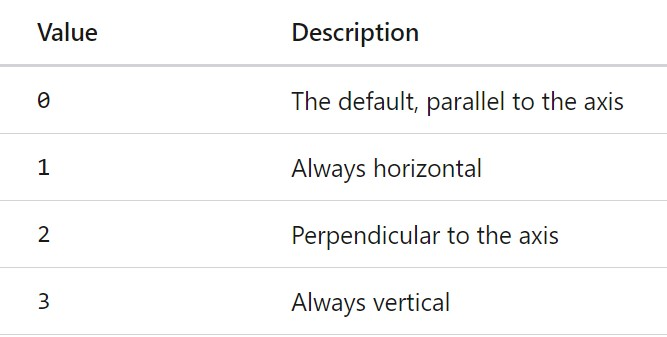
\includegraphics[width=0.55\linewidth]{img01/w01-las} 

}

\caption{Axis label styles in R}\label{fig:unnamed-chunk-9}
\end{figure}

The figure below shows different axis label styles.

\begin{Shaded}
\begin{Highlighting}[]
\FunctionTok{par}\NormalTok{(}\AttributeTok{mfrow =} \FunctionTok{c}\NormalTok{(}\DecValTok{2}\NormalTok{,}\DecValTok{2}\NormalTok{), }\AttributeTok{mar=}\FunctionTok{c}\NormalTok{(}\DecValTok{4}\NormalTok{, }\DecValTok{4}\NormalTok{, }\DecValTok{4}\NormalTok{, }\DecValTok{4}\NormalTok{), }\AttributeTok{oma =} \FunctionTok{c}\NormalTok{(}\FloatTok{0.1}\NormalTok{, }\FloatTok{0.1}\NormalTok{, }\FloatTok{0.1}\NormalTok{, }\FloatTok{0.1}\NormalTok{))}
\FunctionTok{plot}\NormalTok{(x, y, }\AttributeTok{type =} \StringTok{"b"}\NormalTok{, }\AttributeTok{main =} \StringTok{"las = 0"}\NormalTok{, }\AttributeTok{las =} \DecValTok{0}\NormalTok{, }\AttributeTok{xlab =} \StringTok{"x{-}values"}\NormalTok{, }\AttributeTok{ylab=}\StringTok{"y{-}values"}\NormalTok{)}
\FunctionTok{plot}\NormalTok{(x, y, }\AttributeTok{type =} \StringTok{"b"}\NormalTok{, }\AttributeTok{main =} \StringTok{"las = 1"}\NormalTok{, }\AttributeTok{las =} \DecValTok{1}\NormalTok{, }\AttributeTok{xlab =} \StringTok{"x{-}values"}\NormalTok{, }\AttributeTok{ylab=}\StringTok{"y{-}values"}\NormalTok{)}
\FunctionTok{plot}\NormalTok{(x, y, }\AttributeTok{type =} \StringTok{"b"}\NormalTok{, }\AttributeTok{main =} \StringTok{"las = 2"}\NormalTok{, }\AttributeTok{las =} \DecValTok{2}\NormalTok{, }\AttributeTok{xlab =} \StringTok{"x{-}values"}\NormalTok{, }\AttributeTok{ylab=}\StringTok{"y{-}values"}\NormalTok{)}
\FunctionTok{plot}\NormalTok{(x, y, }\AttributeTok{type =} \StringTok{"b"}\NormalTok{, }\AttributeTok{main =} \StringTok{"las = 3"}\NormalTok{, }\AttributeTok{las =} \DecValTok{3}\NormalTok{, }\AttributeTok{xlab =} \StringTok{"x{-}values"}\NormalTok{, }\AttributeTok{ylab=}\StringTok{"y{-}values"}\NormalTok{)}
\end{Highlighting}
\end{Shaded}

\begin{figure}

{\centering 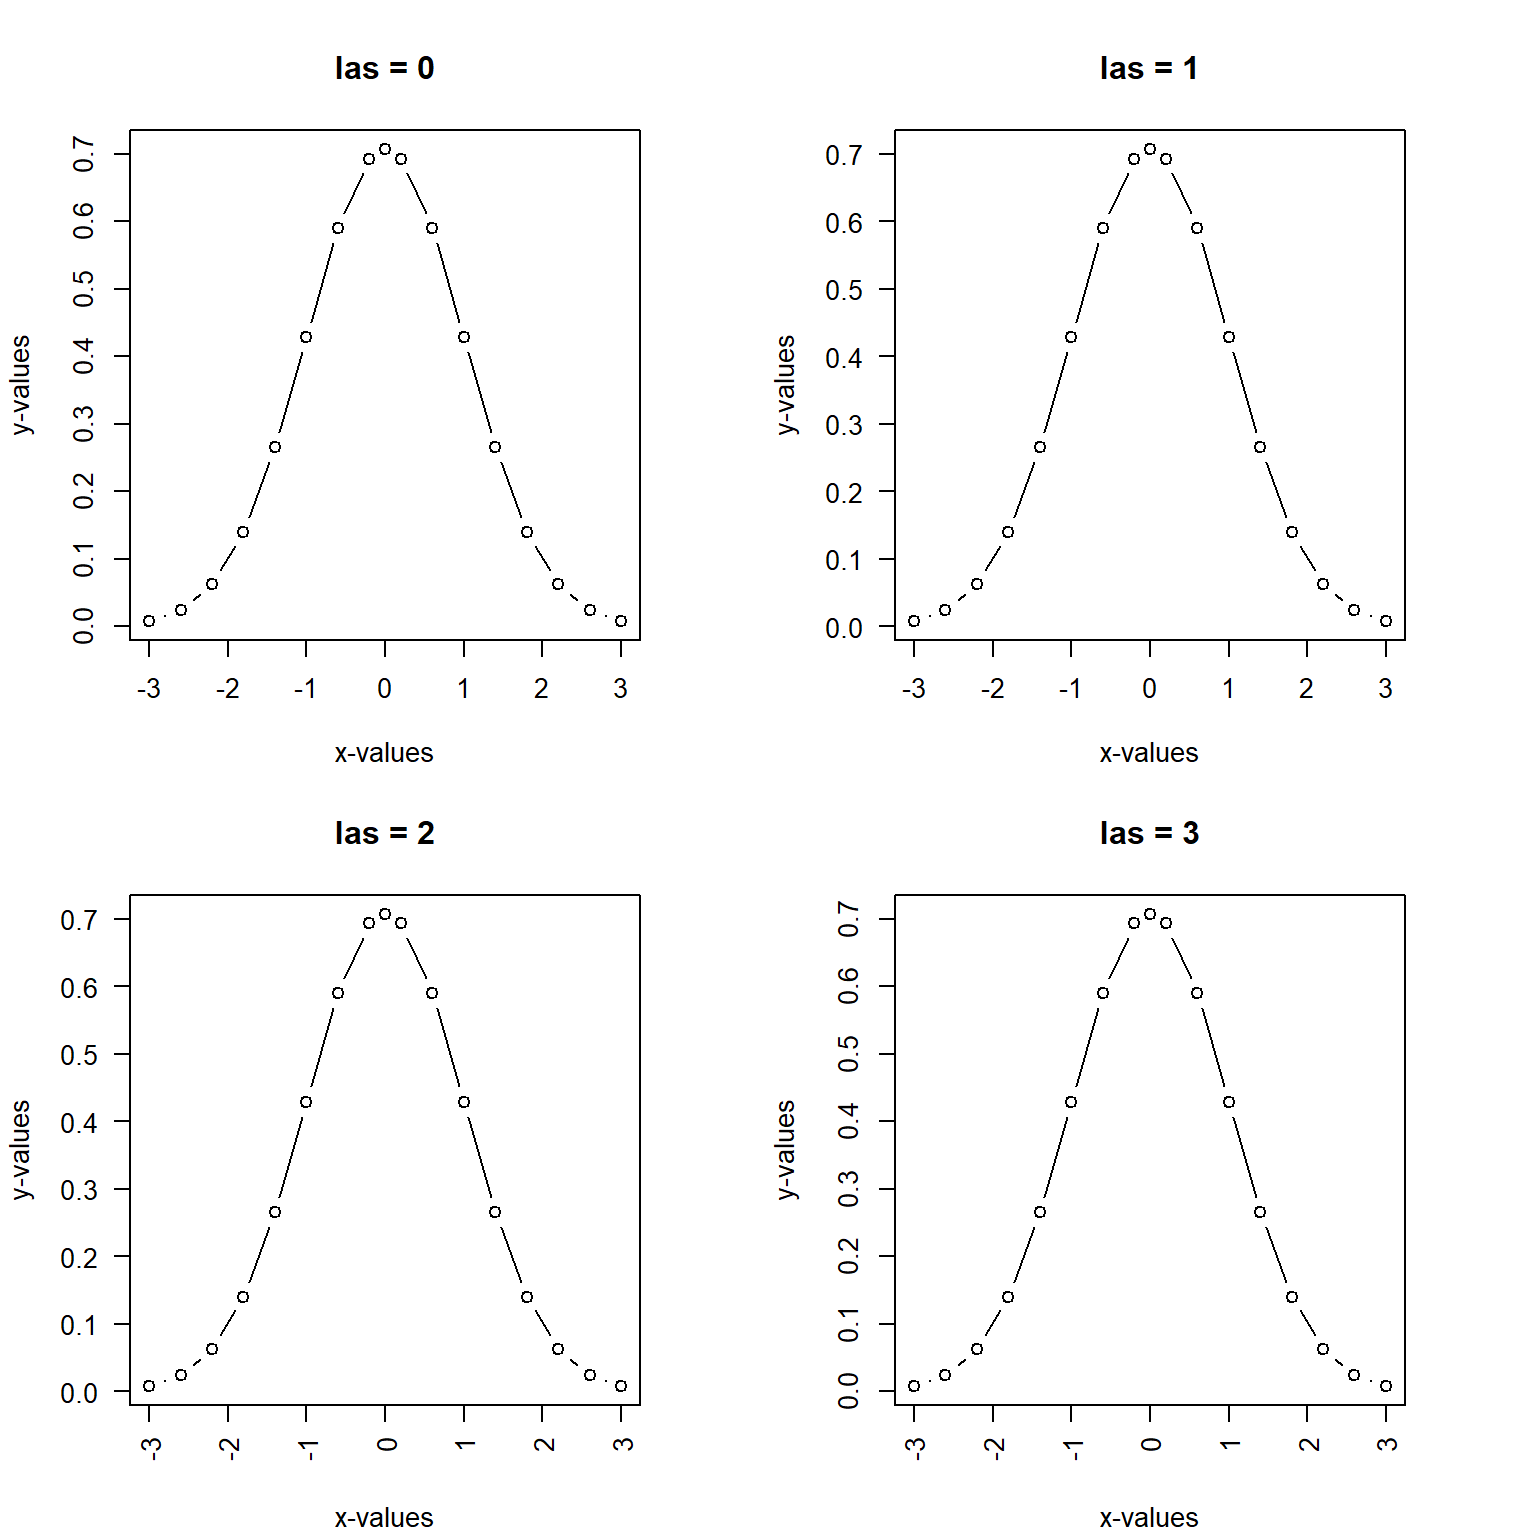
\includegraphics{STA504EB_files/figure-latex/unnamed-chunk-10-1} 

}

\caption{Different shapes in the plot of normal density function}\label{fig:unnamed-chunk-10}
\end{figure}

\hypertarget{r-colors}{%
\subsubsection{R Colors}\label{r-colors}}

R has hundreds of different colors defined based the base colors:RGB. You can use this link to find the color code for your needs: \url{https://rstudio-pubs-static.s3.amazonaws.com/3486_79191ad32cf74955b4502b8530aad627.html}

When plotting, we can use \texttt{col\ =\ colorCode} to specify a color for the plot. For point shapes with code 21-25, you can choose different colors for the border and the background respectively.

The following are few example plots

\begin{Shaded}
\begin{Highlighting}[]
\FunctionTok{par}\NormalTok{(}\AttributeTok{mfrow =} \FunctionTok{c}\NormalTok{(}\DecValTok{2}\NormalTok{,}\DecValTok{2}\NormalTok{), }\AttributeTok{mar=}\FunctionTok{c}\NormalTok{(}\DecValTok{4}\NormalTok{, }\DecValTok{4}\NormalTok{, }\DecValTok{4}\NormalTok{, }\DecValTok{4}\NormalTok{), }\AttributeTok{oma =} \FunctionTok{c}\NormalTok{(}\FloatTok{0.1}\NormalTok{, }\FloatTok{0.1}\NormalTok{, }\FloatTok{0.1}\NormalTok{, }\FloatTok{0.1}\NormalTok{))}
\FunctionTok{plot}\NormalTok{(x, y, }\AttributeTok{type =} \StringTok{"l"}\NormalTok{, }\AttributeTok{main =} \StringTok{"color code: 2"}\NormalTok{,  }\AttributeTok{col =} \DecValTok{2}\NormalTok{,         }
     \AttributeTok{xlab =} \StringTok{"x{-}values"}\NormalTok{, }\AttributeTok{ylab=}\StringTok{"y{-}values"}\NormalTok{)}
\FunctionTok{plot}\NormalTok{(x, y, }\AttributeTok{type =} \StringTok{"l"}\NormalTok{, }\AttributeTok{main =} \StringTok{"color name: blue"}\NormalTok{,    }\AttributeTok{col =} \StringTok{"blue"}\NormalTok{,    }
     \AttributeTok{xlab =} \StringTok{"x{-}values"}\NormalTok{, }\AttributeTok{ylab=}\StringTok{"y{-}values"}\NormalTok{)}
\FunctionTok{plot}\NormalTok{(x, y, }\AttributeTok{type =} \StringTok{"p"}\NormalTok{, }\AttributeTok{main =} \StringTok{"color name: darkred"}\NormalTok{, }\AttributeTok{col =} \StringTok{"darkred"}\NormalTok{, }\AttributeTok{pch=} \DecValTok{22}\NormalTok{,  }
     \AttributeTok{bg =} \StringTok{"yellow"}\NormalTok{, }\AttributeTok{xlab =} \StringTok{"x{-}values"}\NormalTok{, }\AttributeTok{ylab=}\StringTok{"y{-}values"}\NormalTok{)}
\FunctionTok{plot}\NormalTok{(x, y, }\AttributeTok{type =} \StringTok{"p"}\NormalTok{, }\AttributeTok{main =} \StringTok{"color code: 3"}\NormalTok{,  }\AttributeTok{col =} \DecValTok{5}\NormalTok{, }\AttributeTok{pch=} \DecValTok{25}\NormalTok{,  }\AttributeTok{bg =} \StringTok{"red"}\NormalTok{,   }
     \AttributeTok{xlab =} \StringTok{"x{-}values"}\NormalTok{, }\AttributeTok{ylab=}\StringTok{"y{-}values"}\NormalTok{)}
\end{Highlighting}
\end{Shaded}

\begin{figure}

{\centering 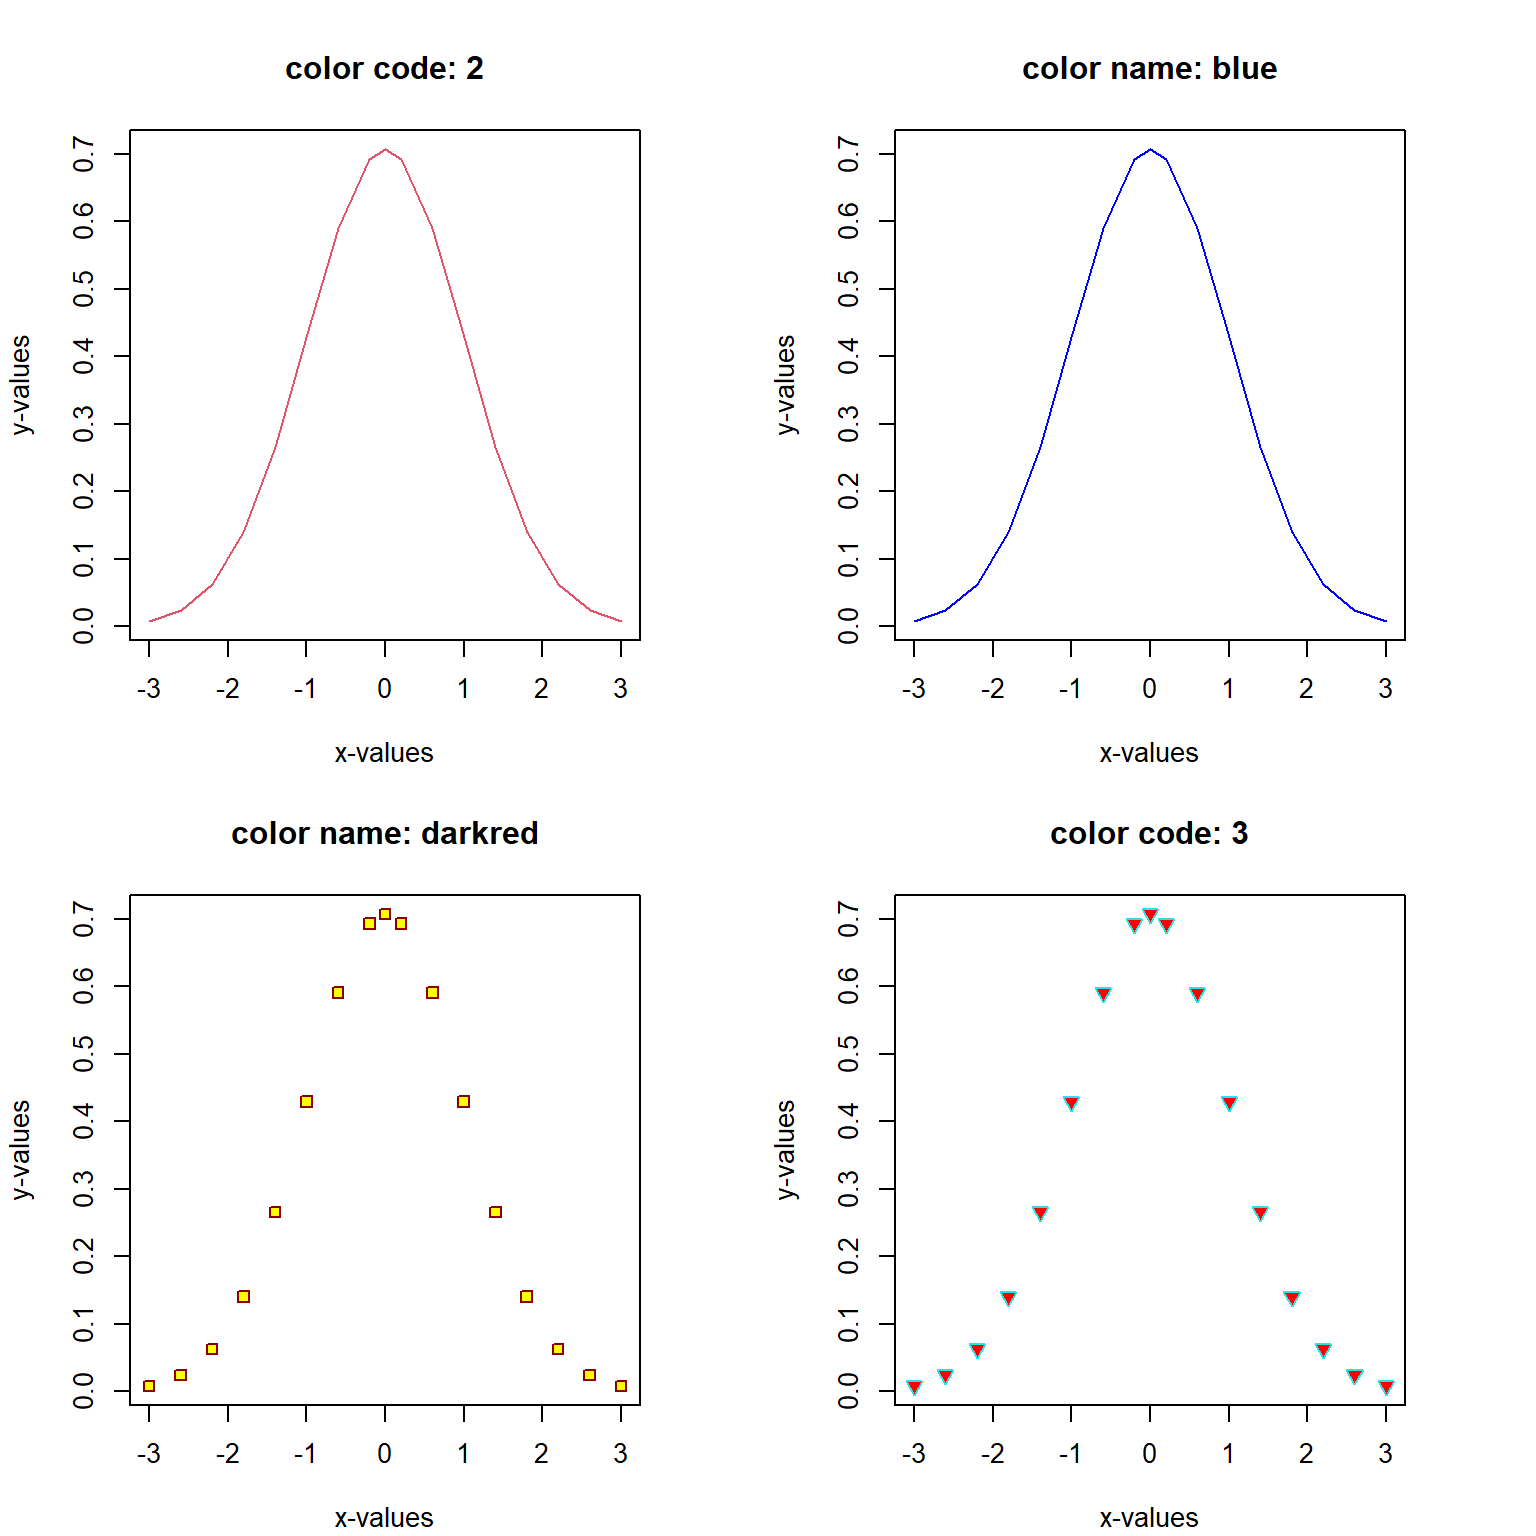
\includegraphics{STA504EB_files/figure-latex/unnamed-chunk-11-1} 

}

\caption{Coloring border and background of points and coloring lines}\label{fig:unnamed-chunk-11}
\end{figure}

\hypertarget{cex---character-expansion}{%
\subsubsection{\texorpdfstring{\texttt{cex} - Character Expansion}{cex - Character Expansion}}\label{cex---character-expansion}}

We can re-scale the the point size of the plot in R. The default size is 1. If the value of \texttt{cex} is less than 1, then the size of the character will be reduced. If assigned value id greater than 1, the size character will be increased.

\begin{Shaded}
\begin{Highlighting}[]
\FunctionTok{par}\NormalTok{(}\AttributeTok{mfrow =} \FunctionTok{c}\NormalTok{(}\DecValTok{1}\NormalTok{,}\DecValTok{2}\NormalTok{), }\AttributeTok{mar=}\FunctionTok{c}\NormalTok{(}\DecValTok{4}\NormalTok{, }\DecValTok{4}\NormalTok{, }\DecValTok{4}\NormalTok{, }\DecValTok{4}\NormalTok{), }\AttributeTok{oma =} \FunctionTok{c}\NormalTok{(}\FloatTok{0.1}\NormalTok{, }\FloatTok{0.1}\NormalTok{, }\FloatTok{0.1}\NormalTok{, }\FloatTok{0.1}\NormalTok{))}
\FunctionTok{plot}\NormalTok{(x, y, }\AttributeTok{type =} \StringTok{"p"}\NormalTok{, }\AttributeTok{main =} \StringTok{"border: darkred, bg: yellow"}\NormalTok{, }\AttributeTok{col =} \StringTok{"darkred"}\NormalTok{, }\AttributeTok{pch=} \DecValTok{21}\NormalTok{,  }
     \AttributeTok{bg =} \StringTok{"yellow"}\NormalTok{, }\AttributeTok{cex =} \FloatTok{1.8}\NormalTok{, }\AttributeTok{xlab =} \StringTok{"x{-}values"}\NormalTok{, }\AttributeTok{ylab=}\StringTok{"y{-}values"}\NormalTok{)}
\FunctionTok{plot}\NormalTok{(x, y, }\AttributeTok{type =} \StringTok{"p"}\NormalTok{, }\AttributeTok{main =} \StringTok{"border: skyblue, bg: red"}\NormalTok{,  }\AttributeTok{col =} \StringTok{"skyblue"}\NormalTok{, }\AttributeTok{pch=} \DecValTok{23}\NormalTok{,  }
     \AttributeTok{bg =} \StringTok{"red"}\NormalTok{, }\AttributeTok{cex =} \FloatTok{0.8}\NormalTok{,  }\AttributeTok{xlab =} \StringTok{"x{-}values"}\NormalTok{, }\AttributeTok{ylab=}\StringTok{"y{-}values"}\NormalTok{)}
\end{Highlighting}
\end{Shaded}

\begin{figure}

{\centering 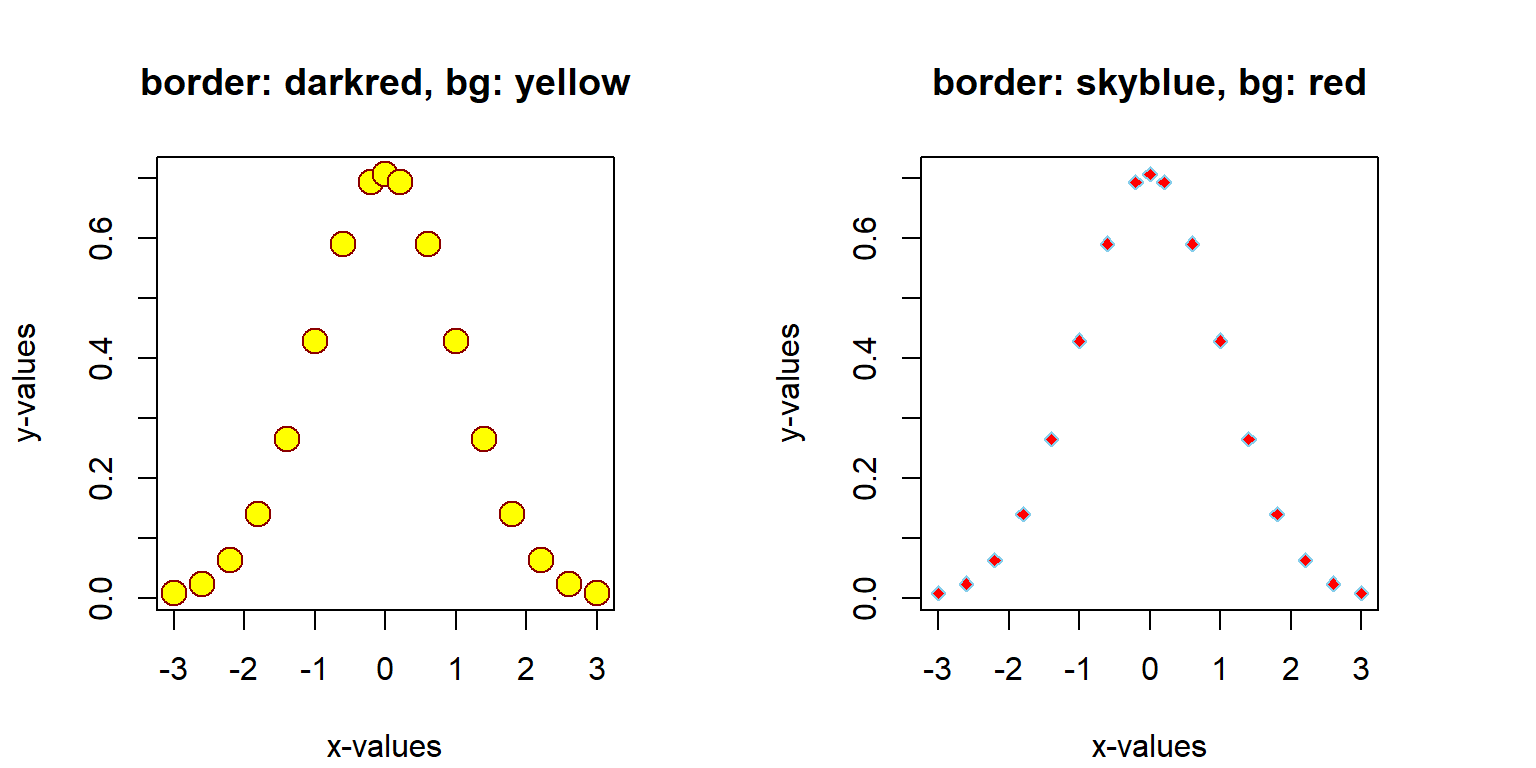
\includegraphics{STA504EB_files/figure-latex/unnamed-chunk-12-1} 

}

\caption{cex: re-size points}\label{fig:unnamed-chunk-12}
\end{figure}

\hypertarget{adding-graphic-components-to-base-plot}{%
\subsection{Adding Graphic Components to Base Plot}\label{adding-graphic-components-to-base-plot}}

The above simple plots are made using the generic plot function \texttt{plot()}. We can use the arguments to choose plot types, point characters, colors, sizes, etc. Sometimes we may want to add additional graphic features using associated graphic functions to make the plot more informative and more aesthetically appealing to viewers.

\hypertarget{adding-a-grid-grid}{%
\subsubsection{\texorpdfstring{Adding A Grid: \texttt{grid()}}{Adding A Grid: grid()}}\label{adding-a-grid-grid}}

\begin{Shaded}
\begin{Highlighting}[]
\FunctionTok{par}\NormalTok{(}\AttributeTok{mfrow =} \FunctionTok{c}\NormalTok{(}\DecValTok{2}\NormalTok{,}\DecValTok{2}\NormalTok{), }\AttributeTok{mar=}\FunctionTok{c}\NormalTok{(}\DecValTok{4}\NormalTok{, }\DecValTok{4}\NormalTok{, }\DecValTok{4}\NormalTok{, }\DecValTok{4}\NormalTok{), }\AttributeTok{oma =} \FunctionTok{c}\NormalTok{(}\FloatTok{0.1}\NormalTok{, }\FloatTok{0.1}\NormalTok{, }\FloatTok{0.1}\NormalTok{, }\FloatTok{0.1}\NormalTok{))}
\FunctionTok{plot}\NormalTok{(x, y, }\AttributeTok{type =} \StringTok{"l"}\NormalTok{, }\AttributeTok{main =} \StringTok{"color code: 2"}\NormalTok{,  }\AttributeTok{col =} \DecValTok{2}\NormalTok{,         }
     \AttributeTok{xlab =} \StringTok{"x{-}values"}\NormalTok{, }\AttributeTok{ylab=}\StringTok{"y{-}values"}\NormalTok{)}
\FunctionTok{grid}\NormalTok{(}\DecValTok{5}\NormalTok{, }\DecValTok{5}\NormalTok{, }\AttributeTok{lty =} \DecValTok{1}\NormalTok{, }\AttributeTok{col =} \StringTok{"red"}\NormalTok{)}


\FunctionTok{plot}\NormalTok{(x, y, }\AttributeTok{type =} \StringTok{"l"}\NormalTok{, }\AttributeTok{main =} \StringTok{"color name: blue"}\NormalTok{,    }\AttributeTok{col =} \StringTok{"blue"}\NormalTok{,    }
     \AttributeTok{xlab =} \StringTok{"x{-}values"}\NormalTok{, }\AttributeTok{ylab=}\StringTok{"y{-}values"}\NormalTok{)}
\FunctionTok{grid}\NormalTok{(}\DecValTok{10}\NormalTok{, }\DecValTok{10}\NormalTok{, }\AttributeTok{lty =} \DecValTok{2}\NormalTok{, }\AttributeTok{col =} \StringTok{"blue"}\NormalTok{)}

\FunctionTok{plot}\NormalTok{(x, y, }\AttributeTok{type =} \StringTok{"p"}\NormalTok{, }\AttributeTok{main =} \StringTok{"color name: darkred"}\NormalTok{, }\AttributeTok{col =} \StringTok{"darkred"}\NormalTok{, }\AttributeTok{pch=} \DecValTok{22}\NormalTok{,  }
     \AttributeTok{bg =} \StringTok{"yellow"}\NormalTok{, }\AttributeTok{xlab =} \StringTok{"x{-}values"}\NormalTok{, }\AttributeTok{ylab=}\StringTok{"y{-}values"}\NormalTok{)}
\FunctionTok{grid}\NormalTok{(}\DecValTok{15}\NormalTok{, }\DecValTok{15}\NormalTok{, }\AttributeTok{lty =} \DecValTok{3}\NormalTok{, }\AttributeTok{col =} \StringTok{"purple"}\NormalTok{)}

\FunctionTok{plot}\NormalTok{(x, y, }\AttributeTok{type =} \StringTok{"p"}\NormalTok{, }\AttributeTok{main =} \StringTok{"color code: 3"}\NormalTok{,  }\AttributeTok{col =} \DecValTok{5}\NormalTok{, }\AttributeTok{pch=} \DecValTok{25}\NormalTok{,  }\AttributeTok{bg =} \StringTok{"red"}\NormalTok{,   }
     \AttributeTok{xlab =} \StringTok{"x{-}values"}\NormalTok{, }\AttributeTok{ylab=}\StringTok{"y{-}values"}\NormalTok{)}
\FunctionTok{grid}\NormalTok{(}\DecValTok{20}\NormalTok{, }\DecValTok{20}\NormalTok{, }\AttributeTok{lty =} \DecValTok{4}\NormalTok{, }\AttributeTok{col =} \StringTok{"darkgreen"}\NormalTok{)}
\end{Highlighting}
\end{Shaded}

\begin{figure}

{\centering 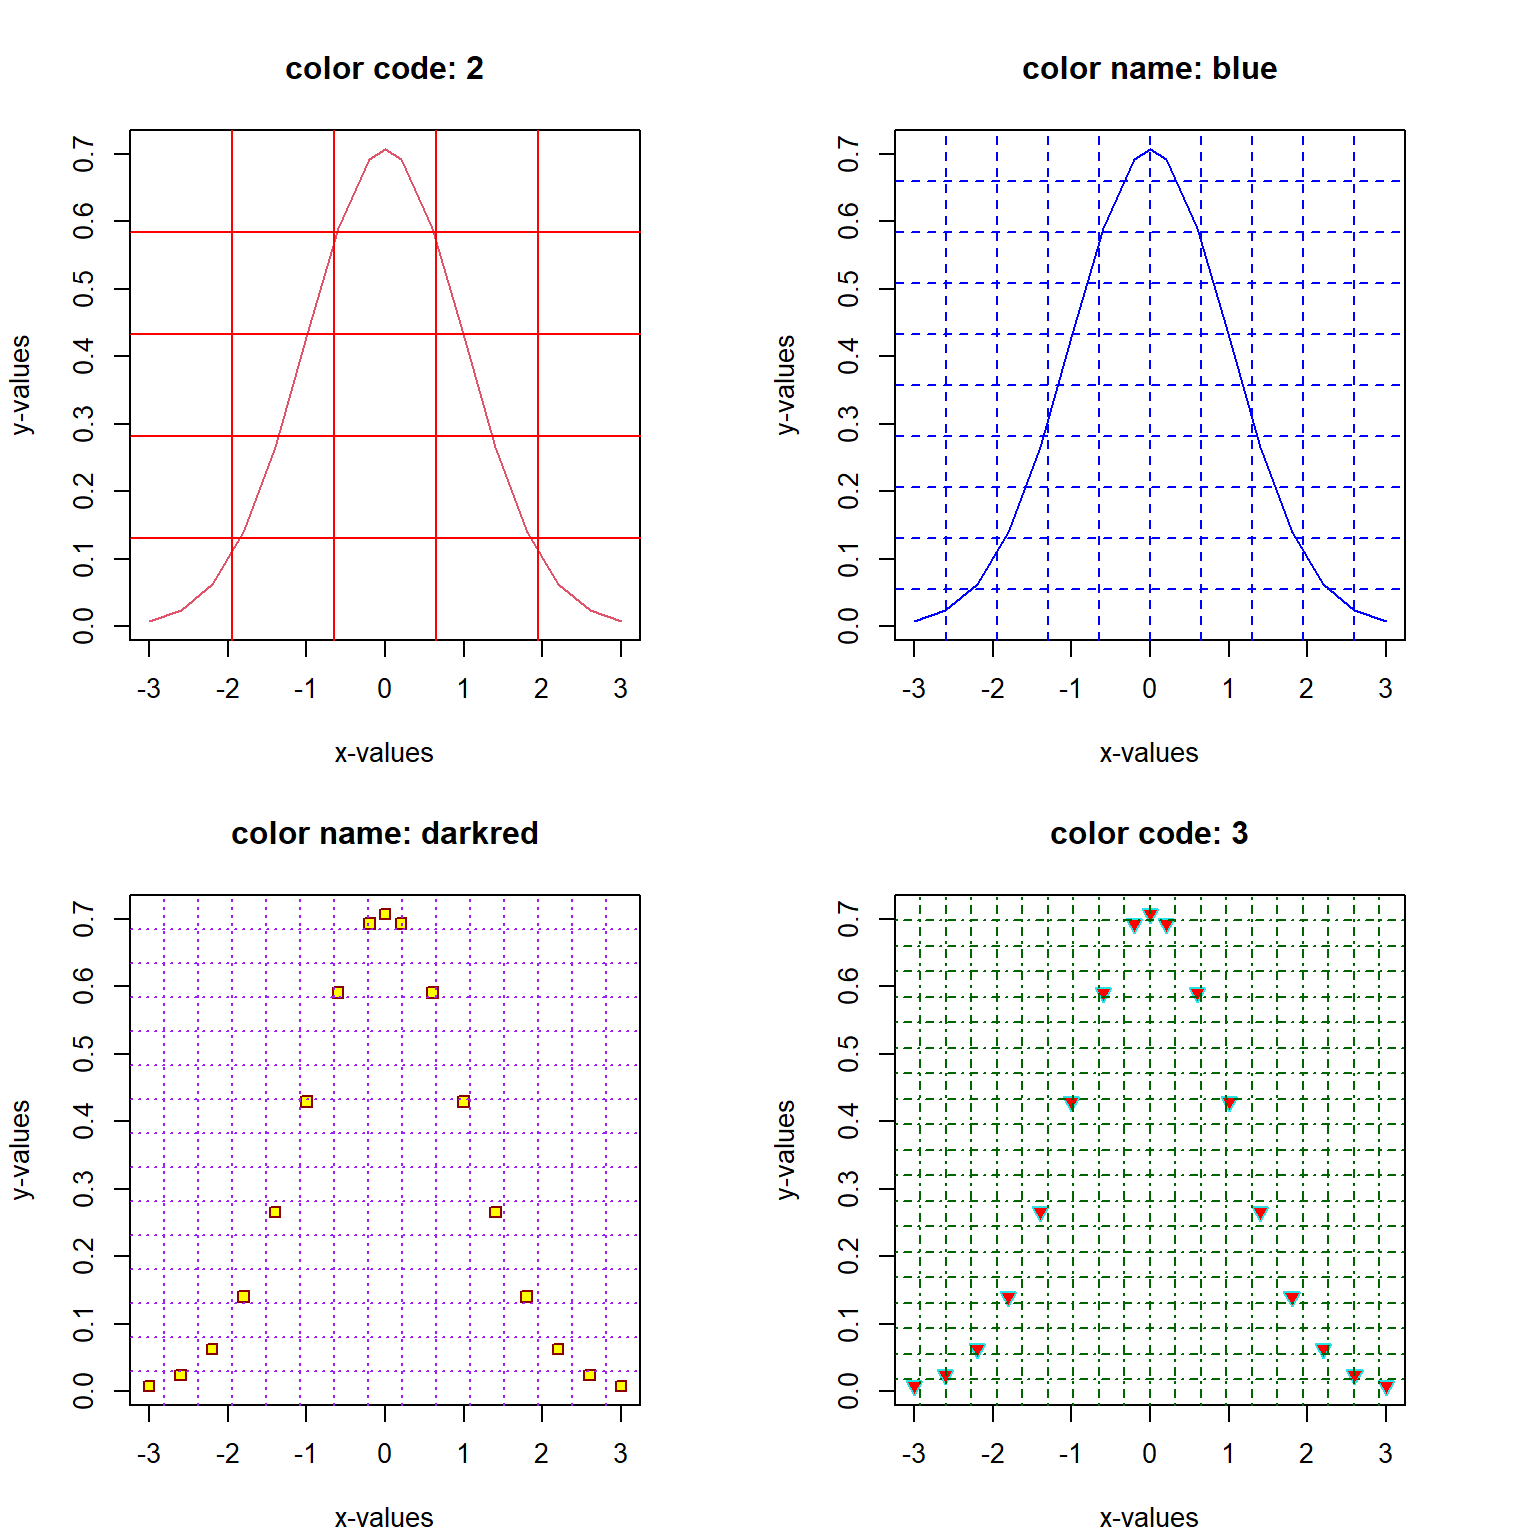
\includegraphics{STA504EB_files/figure-latex/unnamed-chunk-13-1} 

}

\caption{Adding a grid to existing plots}\label{fig:unnamed-chunk-13}
\end{figure}

\hypertarget{add-new-points-and-lines}{%
\subsubsection{Add New Points and Lines}\label{add-new-points-and-lines}}

We can also use graphic function \texttt{points()} and \texttt{lines()} to add points and lines with different features discussed in the generic plot created using the generic \texttt{plot()} function. For example, we can find the point(s) that has (have) the biggest vertical coordinate and then make a line that passes through the origin and the top point(s).

\begin{Shaded}
\begin{Highlighting}[]
\NormalTok{max.id }\OtherTok{=} \FunctionTok{which}\NormalTok{(y}\SpecialCharTok{==}\FunctionTok{max}\NormalTok{(y))}
\NormalTok{max.x }\OtherTok{=}\NormalTok{ x[max.id]}
\NormalTok{max.y }\OtherTok{=}\NormalTok{ y[max.id]}
\FunctionTok{plot}\NormalTok{(x,y, }\AttributeTok{type =} \StringTok{"l"}\NormalTok{, }\AttributeTok{lty =} \DecValTok{1}\NormalTok{, }\AttributeTok{col =} \StringTok{"navy"}\NormalTok{, }\AttributeTok{xlab =} \StringTok{""}\NormalTok{, }\AttributeTok{ylab =} \StringTok{""}\NormalTok{,}
     \AttributeTok{main =} \StringTok{"Normal density curve: highest point(s)"}\NormalTok{)}
\DocumentationTok{\#\# adding points: the origin and the top point!}
\FunctionTok{points}\NormalTok{(}\FunctionTok{c}\NormalTok{(}\DecValTok{0}\NormalTok{,max.x), }\FunctionTok{c}\NormalTok{(}\DecValTok{0}\NormalTok{,max.y), }\AttributeTok{pch =} \DecValTok{21}\NormalTok{, }\AttributeTok{col =} \StringTok{"red"}\NormalTok{, }\AttributeTok{bg =} \StringTok{"yellow"}\NormalTok{, }\AttributeTok{cex =} \DecValTok{2}\NormalTok{)}
\DocumentationTok{\#\# Adding parallel line passing through the top point(s)}
\FunctionTok{lines}\NormalTok{(}\FunctionTok{c}\NormalTok{(}\DecValTok{0}\NormalTok{,max.x), }\FunctionTok{c}\NormalTok{(}\DecValTok{0}\NormalTok{,max.y), }\AttributeTok{lty =} \DecValTok{2}\NormalTok{, }\AttributeTok{col =} \StringTok{"orange"}\NormalTok{)}
\end{Highlighting}
\end{Shaded}

\begin{figure}

{\centering 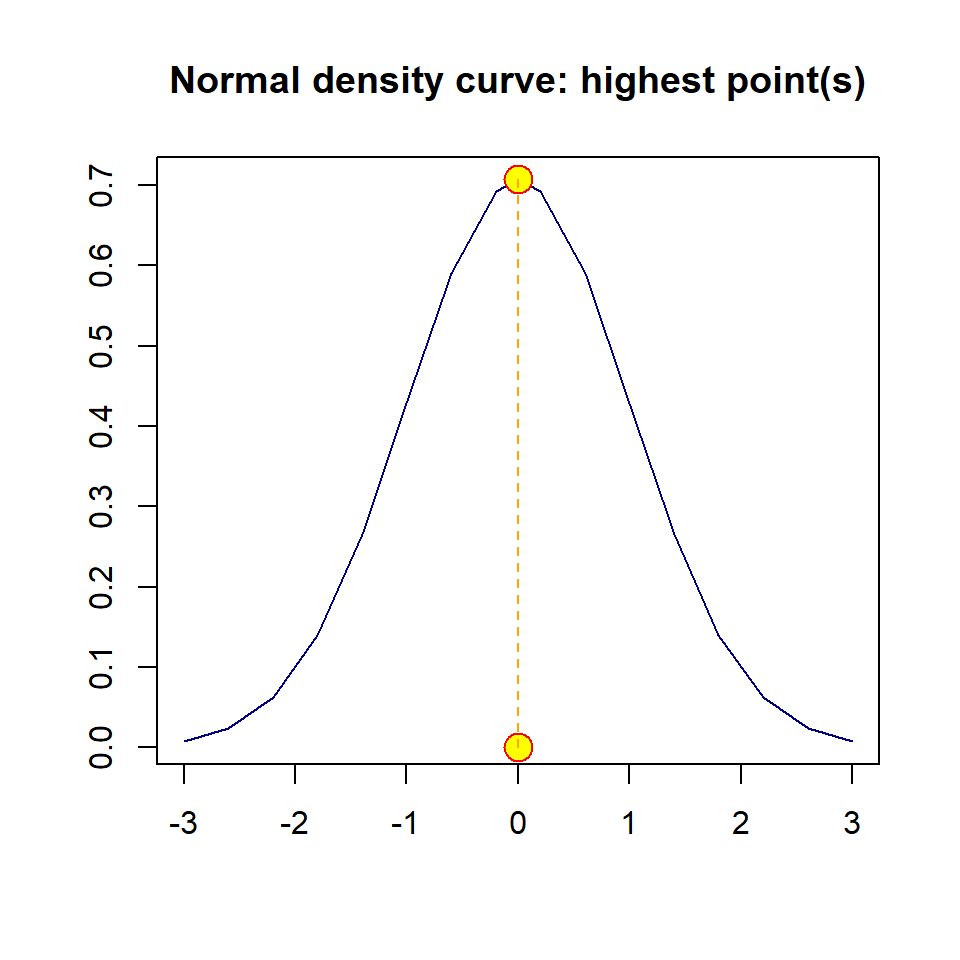
\includegraphics{STA504EB_files/figure-latex/unnamed-chunk-14-1} 

}

\caption{Adding points and lines to the base plot}\label{fig:unnamed-chunk-14}
\end{figure}

\textbf{Note}: If there are only two points, \texttt{abline()} function will do the same trick. If you only want to draw a straight line with given intercept and slop, use \texttt{abline()} and provide the values of intercept and slope. for example, we can add straight line with slope 0.15 and intercept 0.5, the follow code will add the line to the above graph.

\begin{Shaded}
\begin{Highlighting}[]
\FunctionTok{plot}\NormalTok{(x,y, }\AttributeTok{type =} \StringTok{"l"}\NormalTok{, }\AttributeTok{lty =} \DecValTok{1}\NormalTok{, }\AttributeTok{col =} \StringTok{"navy"}\NormalTok{, }\AttributeTok{xlab =} \StringTok{""}\NormalTok{, }\AttributeTok{ylab =} \StringTok{""}\NormalTok{,}
     \AttributeTok{main =} \StringTok{"Normal density curve: highest point(s)"}\NormalTok{)}
\DocumentationTok{\#\# adding pa straight line}
\FunctionTok{abline}\NormalTok{(}\FloatTok{0.5}\NormalTok{, }\FloatTok{0.15}\NormalTok{, }\AttributeTok{lty =} \DecValTok{2}\NormalTok{, }\AttributeTok{col =} \StringTok{"red"}\NormalTok{)}
\DocumentationTok{\#\# add a vertical line passing through the origin}
\FunctionTok{abline}\NormalTok{(}\AttributeTok{v =} \DecValTok{0}\NormalTok{, }\AttributeTok{lty =} \DecValTok{3}\NormalTok{, }\AttributeTok{col =} \StringTok{"purple4"}\NormalTok{)}
\end{Highlighting}
\end{Shaded}

\begin{figure}

{\centering 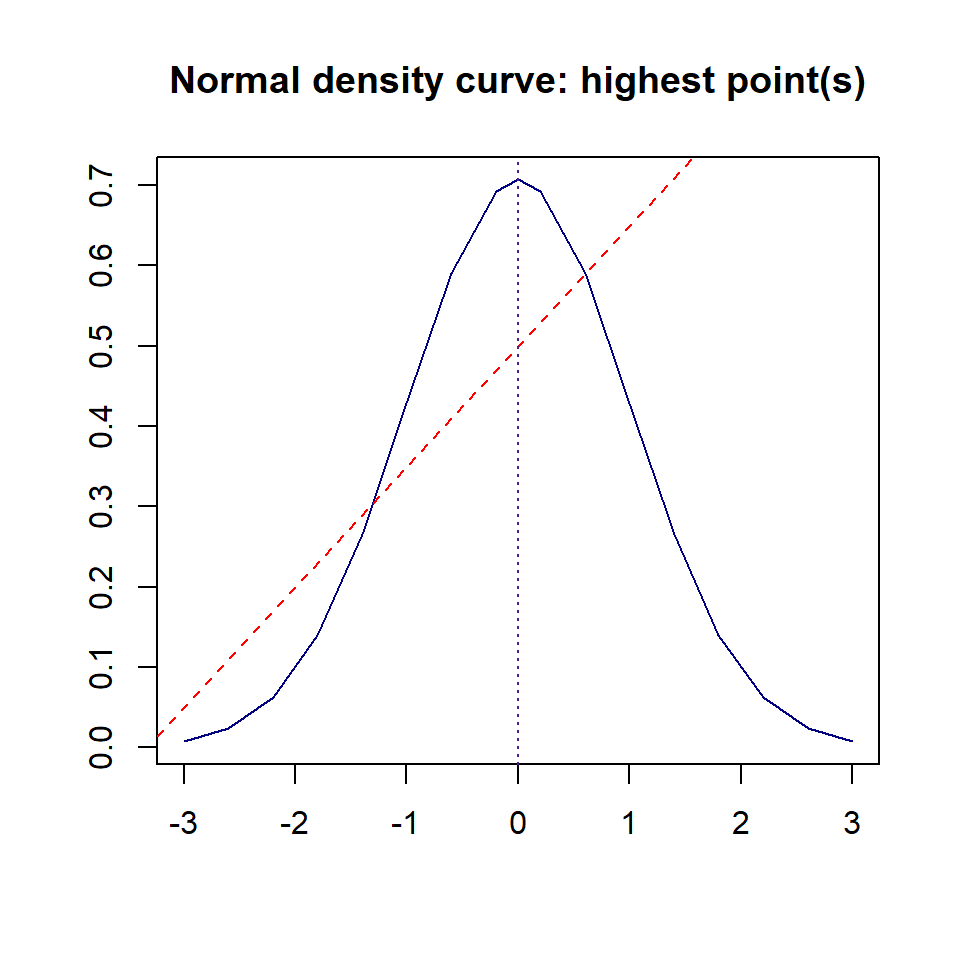
\includegraphics{STA504EB_files/figure-latex/unnamed-chunk-15-1} 

}

\caption{Adding a straight line to the base plot with given intercept and slope}\label{fig:unnamed-chunk-15}
\end{figure}

\hypertarget{add-a-legend}{%
\subsubsection{Add A Legend}\label{add-a-legend}}

If a plot has multiple graphic information, a legend is needed to tell the story. Dependent on the specific plot, we can choose convenient location to place the legend by specifying the x-coordinate and y-coordinate of the center for the legend. There are several special locations that do not need to specify the two coordinates. The following figure shows these special locations.

\begin{figure}

{\centering 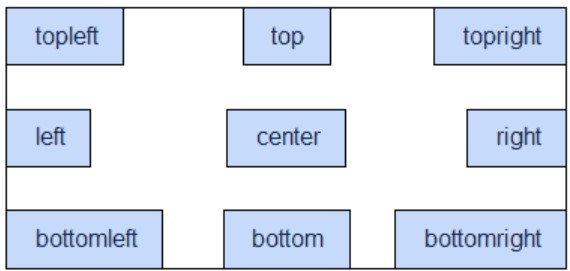
\includegraphics[width=0.55\linewidth]{img01/w01-legendLocations} 

}

\caption{Special locations on a plot to place legend and annotations}\label{fig:unnamed-chunk-16}
\end{figure}

Next, we add a legend to the above plot. The \texttt{topleft} region is the best location to place the legend.

\begin{Shaded}
\begin{Highlighting}[]
\FunctionTok{plot}\NormalTok{(x,y, }\AttributeTok{type =} \StringTok{"l"}\NormalTok{, }\AttributeTok{lty =} \DecValTok{1}\NormalTok{, }\AttributeTok{col =} \StringTok{"navy"}\NormalTok{, }\AttributeTok{xlab =} \StringTok{""}\NormalTok{, }\AttributeTok{ylab =} \StringTok{""}\NormalTok{,}
     \AttributeTok{main =} \StringTok{"Normal density curve: highest point(s)"}\NormalTok{)}
\DocumentationTok{\#\# adding pa straight line}
\FunctionTok{abline}\NormalTok{(}\FloatTok{0.5}\NormalTok{, }\FloatTok{0.15}\NormalTok{, }\AttributeTok{lty =} \DecValTok{2}\NormalTok{, }\AttributeTok{col =} \StringTok{"red"}\NormalTok{)}
\DocumentationTok{\#\# add a vertical line passing through the origin}
\FunctionTok{abline}\NormalTok{(}\AttributeTok{v =} \DecValTok{0}\NormalTok{, }\AttributeTok{lty =} \DecValTok{3}\NormalTok{, }\AttributeTok{col =} \StringTok{"purple4"}\NormalTok{)}
\DocumentationTok{\#\#\#}
\FunctionTok{legend}\NormalTok{(}\StringTok{"topleft"}\NormalTok{, }\FunctionTok{c}\NormalTok{(}\StringTok{"density curve"}\NormalTok{, }\StringTok{"slant line"}\NormalTok{, }\StringTok{"vertical line"}\NormalTok{), }\AttributeTok{lty=}\DecValTok{1}\SpecialCharTok{:}\DecValTok{3}\NormalTok{, }\AttributeTok{col =} \FunctionTok{c}\NormalTok{(}\StringTok{"navy"}\NormalTok{, }\StringTok{"red"}\NormalTok{, }\StringTok{"purple4"}\NormalTok{), }\AttributeTok{cex =} \FloatTok{0.6}\NormalTok{)}
\end{Highlighting}
\end{Shaded}

\begin{figure}

{\centering 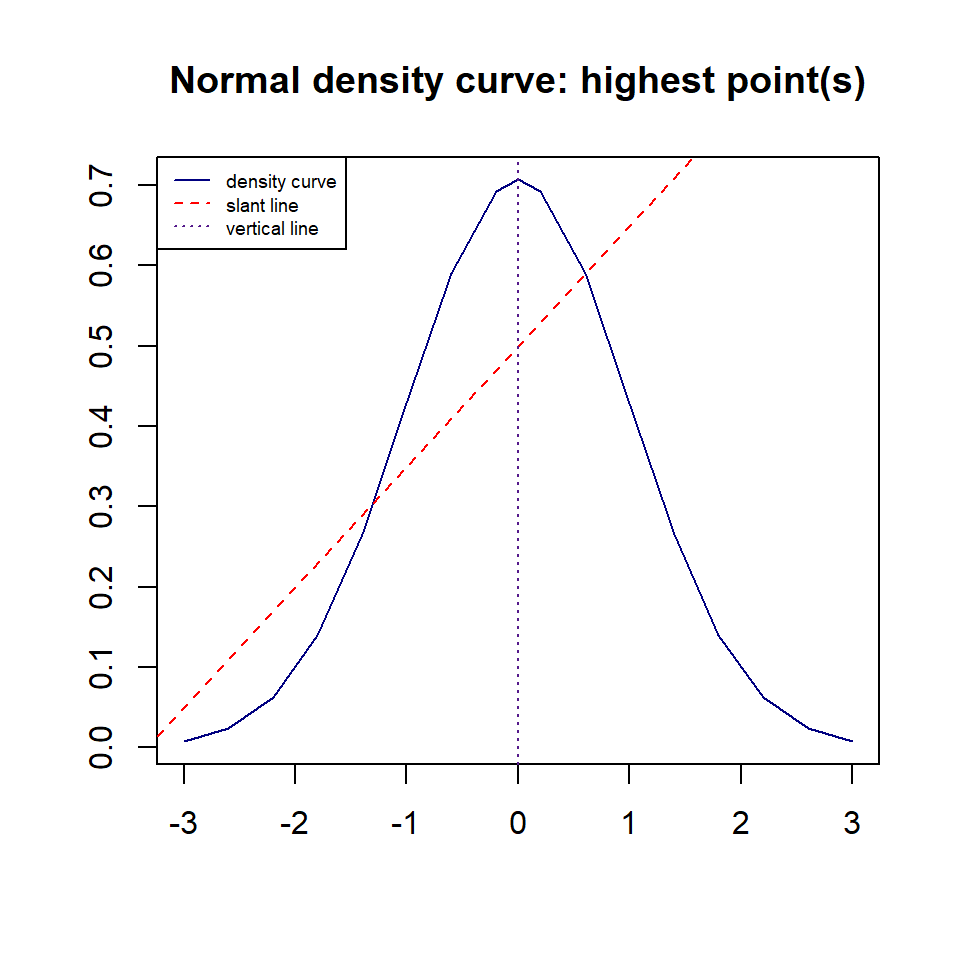
\includegraphics{STA504EB_files/figure-latex/unnamed-chunk-17-1} 

}

\caption{Adding a straight line to the base plot with given intercept and slope}\label{fig:unnamed-chunk-17}
\end{figure}

\hypertarget{add-line-segments-arrows-and-annotations}{%
\subsubsection{Add Line Segments, Arrows and annotations}\label{add-line-segments-arrows-and-annotations}}

Sometimes, we need to draw straight lines between two points to highlight specific information. If highlight a specific point or specific curve, we may need arrow to point to the point or curve and then make an annotation (to be illustrated next).

\begin{Shaded}
\begin{Highlighting}[]
\FunctionTok{plot}\NormalTok{(x,y, }\AttributeTok{type =} \StringTok{"l"}\NormalTok{, }\AttributeTok{lty =} \DecValTok{1}\NormalTok{, }\AttributeTok{col =} \StringTok{"navy"}\NormalTok{, }\AttributeTok{xlab =} \StringTok{""}\NormalTok{, }\AttributeTok{ylab =} \StringTok{""}\NormalTok{,}
     \AttributeTok{main =} \StringTok{"Normal density curve, straight line and line segment"}\NormalTok{)}
\DocumentationTok{\#\# adding pa straight line}
\FunctionTok{points}\NormalTok{(}\FunctionTok{c}\NormalTok{(x[}\DecValTok{3}\NormalTok{], x[}\DecValTok{11}\NormalTok{]), }\FunctionTok{c}\NormalTok{(y[}\DecValTok{3}\NormalTok{], y[}\DecValTok{11}\NormalTok{]), }\AttributeTok{pch =} \DecValTok{21}\NormalTok{, }\AttributeTok{col=}\StringTok{"darkred"}\NormalTok{, }\AttributeTok{bg =} \StringTok{"yellow"}\NormalTok{, }\AttributeTok{cex =} \FloatTok{1.5}\NormalTok{)}
\FunctionTok{segments}\NormalTok{(x[}\DecValTok{3}\NormalTok{], y[}\DecValTok{3}\NormalTok{], x[}\DecValTok{11}\NormalTok{], y[}\DecValTok{11}\NormalTok{], }\AttributeTok{lwd =} \DecValTok{2}\NormalTok{, }\AttributeTok{col =} \StringTok{"red"}\NormalTok{)}
\DocumentationTok{\#\# add a vertical line passing through the origin}
\FunctionTok{abline}\NormalTok{(}\AttributeTok{v =} \DecValTok{0}\NormalTok{, }\AttributeTok{lty =} \DecValTok{3}\NormalTok{, }\AttributeTok{col =} \StringTok{"purple4"}\NormalTok{)}
\DocumentationTok{\#\#\#}
\FunctionTok{legend}\NormalTok{(}\StringTok{"topleft"}\NormalTok{, }\FunctionTok{c}\NormalTok{(}\StringTok{"density curve"}\NormalTok{, }\StringTok{"Line Segment"}\NormalTok{, }\StringTok{"vertical line"}\NormalTok{), }\AttributeTok{lty=}\DecValTok{1}\SpecialCharTok{:}\DecValTok{3}\NormalTok{, }\AttributeTok{col =} \FunctionTok{c}\NormalTok{(}\StringTok{"navy"}\NormalTok{, }\StringTok{"red"}\NormalTok{, }\StringTok{"purple4"}\NormalTok{), }\AttributeTok{cex =} \FloatTok{0.6}\NormalTok{)}
\DocumentationTok{\#\#\#}
\FunctionTok{arrows}\NormalTok{(}\FloatTok{0.5}\NormalTok{, }\FloatTok{0.2}\NormalTok{, }\SpecialCharTok{{-}}\FloatTok{0.5}\NormalTok{, }\FloatTok{0.38}\NormalTok{,  }\AttributeTok{length =} \FloatTok{0.1}\NormalTok{, }\AttributeTok{angle =} \DecValTok{25}\NormalTok{, }\AttributeTok{lty =} \DecValTok{1}\NormalTok{, }\AttributeTok{lwd =} \DecValTok{2}\NormalTok{, }\AttributeTok{col =} \StringTok{"blue"}\NormalTok{)}
\DocumentationTok{\#\#\# annotations}
\FunctionTok{text}\NormalTok{(}\FloatTok{0.5}\NormalTok{, }\FloatTok{0.15}\NormalTok{, }\StringTok{"line segment"}\NormalTok{, }\AttributeTok{col =} \StringTok{"red"}\NormalTok{, }\AttributeTok{cex =} \FloatTok{0.8}\NormalTok{)}
\end{Highlighting}
\end{Shaded}

\begin{figure}

{\centering 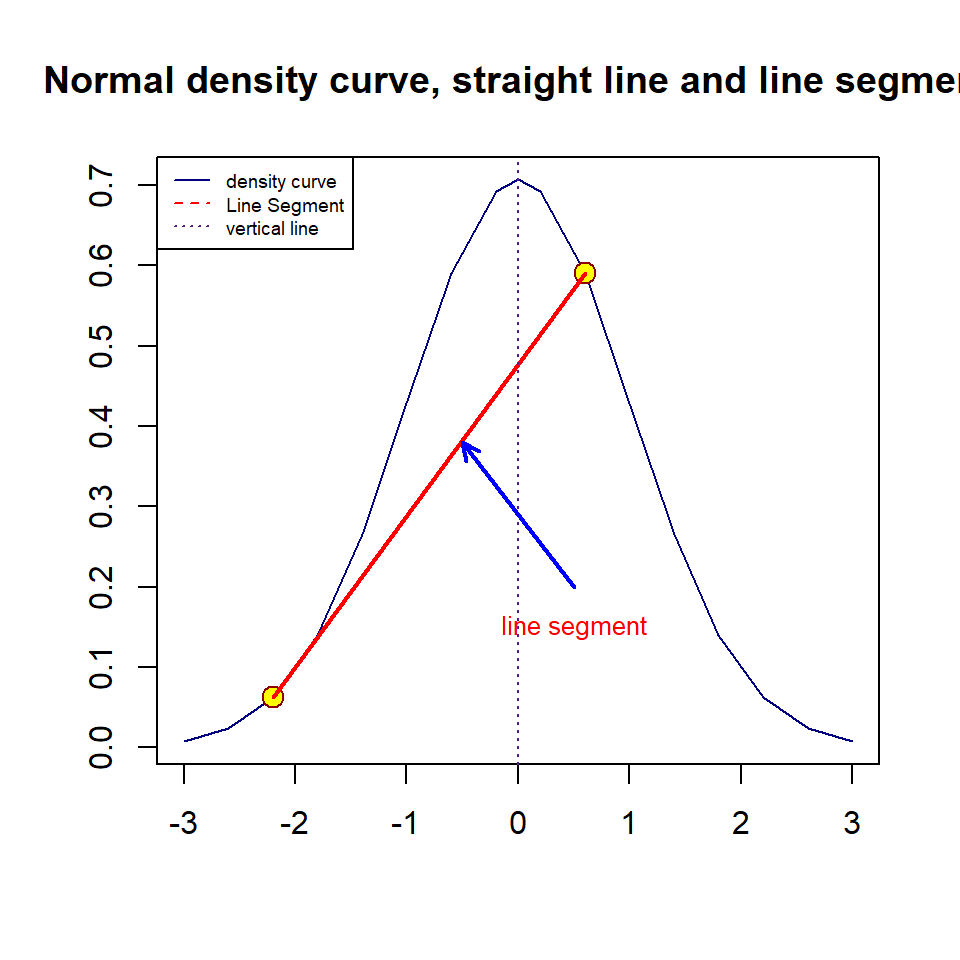
\includegraphics{STA504EB_files/figure-latex/unnamed-chunk-18-1} 

}

\caption{curve, straight line, and line segment}\label{fig:unnamed-chunk-18}
\end{figure}

\hypertarget{additional-arguments-in-plot}{%
\subsubsection{\texorpdfstring{Additional Arguments in \texttt{plot()}}{Additional Arguments in plot()}}\label{additional-arguments-in-plot}}

Sometimes, we may have a long title to explain the plot. R will truncate the long title. This will lead to a partial title. There different ways to get this around. We can change the font size of the title, we could also use multiple line title. For example, we next change the title of the above plot to reflect the information in the plot.

\begin{Shaded}
\begin{Highlighting}[]
\FunctionTok{plot}\NormalTok{(x,y, }\AttributeTok{type =} \StringTok{"l"}\NormalTok{, }\AttributeTok{lty =} \DecValTok{1}\NormalTok{, }\AttributeTok{col =} \StringTok{"navy"}\NormalTok{, }\AttributeTok{xlab =} \StringTok{""}\NormalTok{, }\AttributeTok{ylab =} \StringTok{""}\NormalTok{,}
     \AttributeTok{main =} \StringTok{"Normal density curve, vertical line, line sement, arrows to annotate the straight line"}\NormalTok{)}
\DocumentationTok{\#\# adding pa straight line}
\FunctionTok{points}\NormalTok{(}\FunctionTok{c}\NormalTok{(x[}\DecValTok{3}\NormalTok{], x[}\DecValTok{11}\NormalTok{]), }\FunctionTok{c}\NormalTok{(y[}\DecValTok{3}\NormalTok{], y[}\DecValTok{11}\NormalTok{]), }\AttributeTok{pch =} \DecValTok{21}\NormalTok{, }\AttributeTok{col=}\StringTok{"darkred"}\NormalTok{, }\AttributeTok{bg =} \StringTok{"yellow"}\NormalTok{,}
       \AttributeTok{cex =} \FloatTok{1.5}\NormalTok{)}
\FunctionTok{segments}\NormalTok{(x[}\DecValTok{3}\NormalTok{], y[}\DecValTok{3}\NormalTok{], x[}\DecValTok{11}\NormalTok{], y[}\DecValTok{11}\NormalTok{], }\AttributeTok{lwd =} \DecValTok{2}\NormalTok{, }\AttributeTok{col =} \StringTok{"red"}\NormalTok{)}
\DocumentationTok{\#\# add a vertical line passing through the origin}
\FunctionTok{abline}\NormalTok{(}\AttributeTok{v =} \DecValTok{0}\NormalTok{, }\AttributeTok{lty =} \DecValTok{3}\NormalTok{, }\AttributeTok{col =} \StringTok{"purple4"}\NormalTok{)}
\DocumentationTok{\#\#\#}
\FunctionTok{legend}\NormalTok{(}\StringTok{"topleft"}\NormalTok{, }\FunctionTok{c}\NormalTok{(}\StringTok{"density curve"}\NormalTok{, }\StringTok{"Line segment"}\NormalTok{, }\StringTok{"vertical line"}\NormalTok{), }\AttributeTok{lty=}\DecValTok{1}\SpecialCharTok{:}\DecValTok{3}\NormalTok{, }
       \AttributeTok{col =} \FunctionTok{c}\NormalTok{(}\StringTok{"navy"}\NormalTok{, }\StringTok{"red"}\NormalTok{, }\StringTok{"purple4"}\NormalTok{), }\AttributeTok{cex =} \FloatTok{0.6}\NormalTok{)  }
\FunctionTok{arrows}\NormalTok{(}\FloatTok{0.5}\NormalTok{, }\FloatTok{0.2}\NormalTok{, }\SpecialCharTok{{-}}\FloatTok{0.5}\NormalTok{, }\FloatTok{0.38}\NormalTok{,  }\AttributeTok{length =} \FloatTok{0.1}\NormalTok{, }\AttributeTok{angle =} \DecValTok{25}\NormalTok{, }\AttributeTok{lty =} \DecValTok{1}\NormalTok{, }\AttributeTok{lwd =} \DecValTok{2}\NormalTok{, }
       \AttributeTok{col =} \StringTok{"blue"}\NormalTok{)}
\DocumentationTok{\#\#\# annotations}
\FunctionTok{text}\NormalTok{(}\FloatTok{0.5}\NormalTok{, }\FloatTok{0.15}\NormalTok{, }\StringTok{"line segment"}\NormalTok{, }\AttributeTok{col =} \StringTok{"red"}\NormalTok{, }\AttributeTok{cex =} \FloatTok{0.8}\NormalTok{)}
\end{Highlighting}
\end{Shaded}

\begin{figure}

{\centering 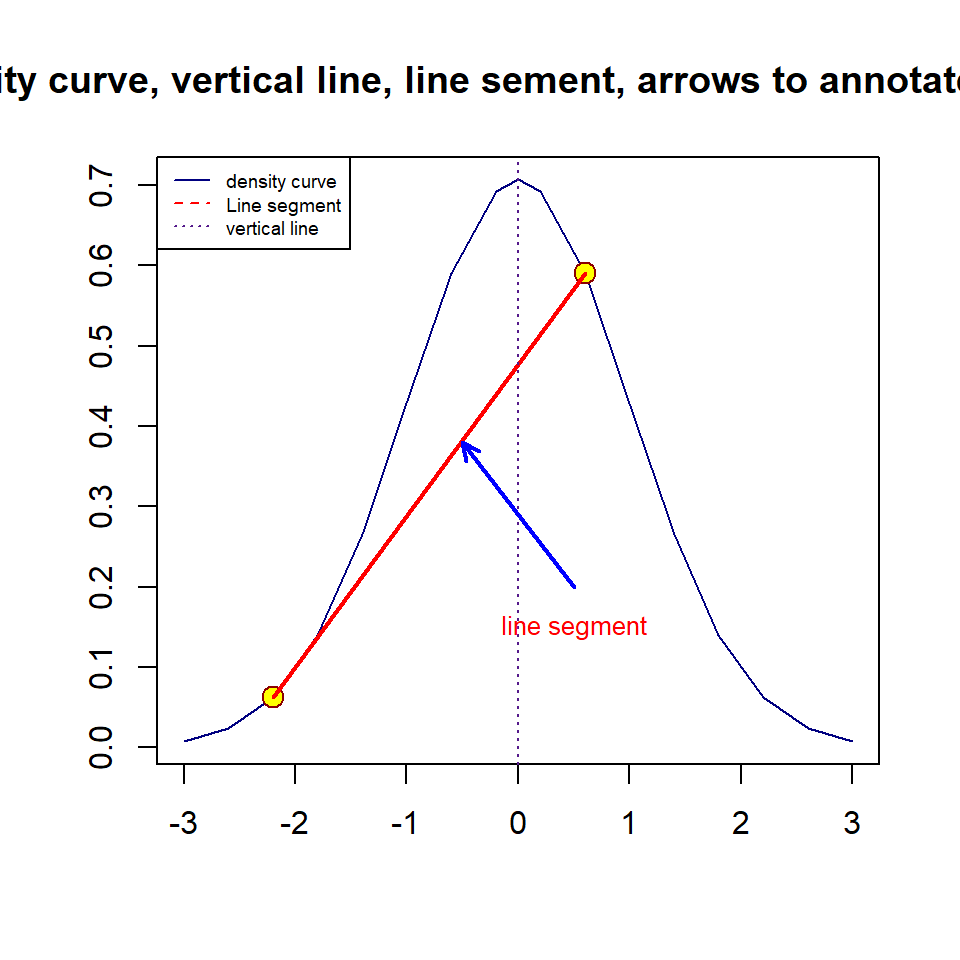
\includegraphics{STA504EB_files/figure-latex/unnamed-chunk-19-1} 

}

\caption{Plot with an annotation and long title}\label{fig:unnamed-chunk-19}
\end{figure}

We next use multiple line title and modify the font size and color to make a nice title.

\begin{Shaded}
\begin{Highlighting}[]
\FunctionTok{plot}\NormalTok{(x,y, }\AttributeTok{type =} \StringTok{"l"}\NormalTok{, }\AttributeTok{lty =} \DecValTok{1}\NormalTok{, }\AttributeTok{col =} \StringTok{"navy"}\NormalTok{, }\AttributeTok{xlab =} \StringTok{""}\NormalTok{, }\AttributeTok{ylab =} \StringTok{""}\NormalTok{,}
     \AttributeTok{main =} \StringTok{"Normal density curve, vertical line, line sement, }
\StringTok{             arrows to annotate the straight line"}\NormalTok{,}
     \AttributeTok{cex.main =} \FloatTok{0.8}\NormalTok{, }\AttributeTok{col.main =} \StringTok{"navy"}\NormalTok{)}
\DocumentationTok{\#\# adding pa straight line}
\FunctionTok{points}\NormalTok{(}\FunctionTok{c}\NormalTok{(x[}\DecValTok{3}\NormalTok{], x[}\DecValTok{11}\NormalTok{]), }\FunctionTok{c}\NormalTok{(y[}\DecValTok{3}\NormalTok{], y[}\DecValTok{11}\NormalTok{]), }\AttributeTok{pch =} \DecValTok{21}\NormalTok{, }\AttributeTok{col=}\StringTok{"darkred"}\NormalTok{, }\AttributeTok{bg =} \StringTok{"yellow"}\NormalTok{, }
       \AttributeTok{cex =} \FloatTok{1.5}\NormalTok{)}
\FunctionTok{segments}\NormalTok{(x[}\DecValTok{3}\NormalTok{], y[}\DecValTok{3}\NormalTok{], x[}\DecValTok{11}\NormalTok{], y[}\DecValTok{11}\NormalTok{], }\AttributeTok{lwd =} \DecValTok{2}\NormalTok{, }\AttributeTok{col =} \StringTok{"red"}\NormalTok{)}
\DocumentationTok{\#\# add a vertical line passing through the origin}
\FunctionTok{abline}\NormalTok{(}\AttributeTok{v =} \DecValTok{0}\NormalTok{, }\AttributeTok{lty =} \DecValTok{3}\NormalTok{, }\AttributeTok{col =} \StringTok{"purple4"}\NormalTok{)}
\DocumentationTok{\#\#\#  bty = "n" removes the box around the legend!}
\FunctionTok{legend}\NormalTok{(}\StringTok{"topleft"}\NormalTok{, }\FunctionTok{c}\NormalTok{(}\StringTok{"density curve"}\NormalTok{, }\StringTok{"Line segment"}\NormalTok{, }\StringTok{"vertical line"}\NormalTok{), }\AttributeTok{lty=}\DecValTok{1}\SpecialCharTok{:}\DecValTok{3}\NormalTok{, }
       \AttributeTok{col =} \FunctionTok{c}\NormalTok{(}\StringTok{"navy"}\NormalTok{, }\StringTok{"red"}\NormalTok{, }\StringTok{"purple4"}\NormalTok{), }\AttributeTok{cex =} \FloatTok{0.6}\NormalTok{, }\AttributeTok{bty =} \StringTok{"n"}\NormalTok{)}
\DocumentationTok{\#\#\#}
\FunctionTok{arrows}\NormalTok{(}\FloatTok{0.5}\NormalTok{, }\FloatTok{0.2}\NormalTok{, }\SpecialCharTok{{-}}\FloatTok{0.5}\NormalTok{, }\FloatTok{0.38}\NormalTok{,  }\AttributeTok{length =} \FloatTok{0.1}\NormalTok{, }\AttributeTok{angle =} \DecValTok{25}\NormalTok{, }\AttributeTok{lty =} \DecValTok{1}\NormalTok{, }\AttributeTok{lwd =} \DecValTok{2}\NormalTok{, }
       \AttributeTok{col =} \StringTok{"blue"}\NormalTok{)}
\DocumentationTok{\#\#\# annotations}
\FunctionTok{text}\NormalTok{(}\FloatTok{0.5}\NormalTok{, }\FloatTok{0.15}\NormalTok{, }\StringTok{"line segment"}\NormalTok{, }\AttributeTok{col =} \StringTok{"red"}\NormalTok{, }\AttributeTok{cex =} \FloatTok{0.8}\NormalTok{)}
\end{Highlighting}
\end{Shaded}

\begin{figure}

{\centering 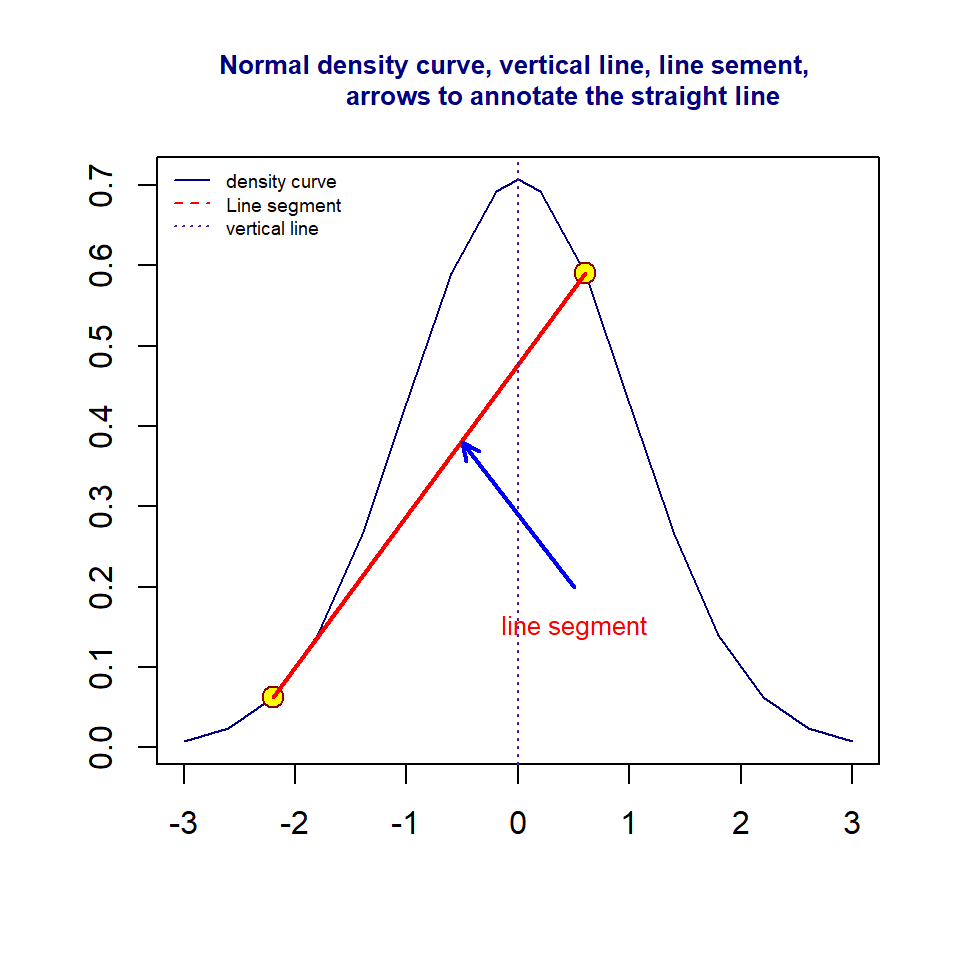
\includegraphics{STA504EB_files/figure-latex/unnamed-chunk-20-1} 

}

\caption{Plot with an annotation and long title}\label{fig:unnamed-chunk-20}
\end{figure}

\hfill\break

With above basics of RMarkdown, LaTex style of mathematics equations, and generic plot functions in R, we should be able to prepare your assignments in a professional digital manner.

\hypertarget{review-of-probability-rules}{%
\chapter{Review of Probability Rules}\label{review-of-probability-rules}}

This note reviews the basic concepts of probability and important probability rules.

\hypertarget{definitions-of-probability}{%
\section{Definitions of Probability}\label{definitions-of-probability}}

In general, probability is a measure of the likelihood of some outcome. We use it not to describe what will happen in one particular event, but rather, what the long-term proportion of that outcome will occur.

\hypertarget{experiments-sample-space-and-event}{%
\subsection{Experiments, Sample Space, and Event}\label{experiments-sample-space-and-event}}

In probability, \textbf{an experiment} is any process where the results are uncertain. We call the \textbf{sample space}, S, the collection of all possible outcomes. A \textbf{probability event} is any collection of outcomes from the experiment.

\textbf{Example 1}: Suppose we have a family with three children, and we consider the sex of those three children.

\textbf{Solution}: If we let B represent a boy and G represent a girl, here is the sample space:

\[S = \{ BBB, BBG, BGB, GBB, BGG, GBG, GGB, GGG\}\]

There are thus 8 outcomes in this experiment. One possible event might be:

E = the family has exactly two girls = \(\{ BGG, GBG, GGB \}\)

\textbf{Unusual Events}: Typically, we say that an event with a probability less than 5\% is \textbf{unusual}, but this isn't a hard cutoff. It depends on the context

Suppose we're planning on making a decision one way unless the probability of a particularly ``unusual'' event is too high. For example, suppose we're planning a picnic on a nice summer day. If the risk of a rain shower isn't too high, we'll plan on the picnic. In this case, we might set our cutoff at 20\% - anything less than that is too unusual (or unlikely) to happen, so we'll risk it.

\hypertarget{calculation-of-probability}{%
\subsection{Calculation of Probability}\label{calculation-of-probability}}

There are two primary methods for calculating probabilities

\textbf{Frequency Approach}: The first is to simply look at what has happened in the past and assume the probability is the same as the \textbf{relative frequency} of that particular outcome. This is called the empirical probability of that event.

\hfill\break

P(E) \(\approx\) relative frequency of E = (frequency of E)/ (total number of trials)

\hfill\break

\textbf{Example 2}: In a statistics class, 38 out of 50 students earned a grade of B or better (denoting this event as an event E). By the above definition, we have \(P(E) \approx 33/60 = 0.55\).

\textbf{Classic Approach}: The second primary method for calculating probabilities is the \textbf{classical method}. The key to this method is to assume that all outcomes are equally likely.

\hfill\break

P(E) = (number of ways E can occur)/(total number of possible outcomes) = N(E)/ N(S)

\hfill\break

\textbf{Example 3}: Let's consider again the probability experiment of rolling two fair six-sided dice. Let the event E = the sum of the two dice is 6. Find P(E)

\textbf{Solution} We first list the elements in the sample space.

\begin{Shaded}
\begin{Highlighting}[]
\NormalTok{knitr}\SpecialCharTok{::}\FunctionTok{include\_graphics}\NormalTok{(}\StringTok{"topic01/sixSidedDice.png"}\NormalTok{)}
\end{Highlighting}
\end{Shaded}

\begin{figure}

{\centering 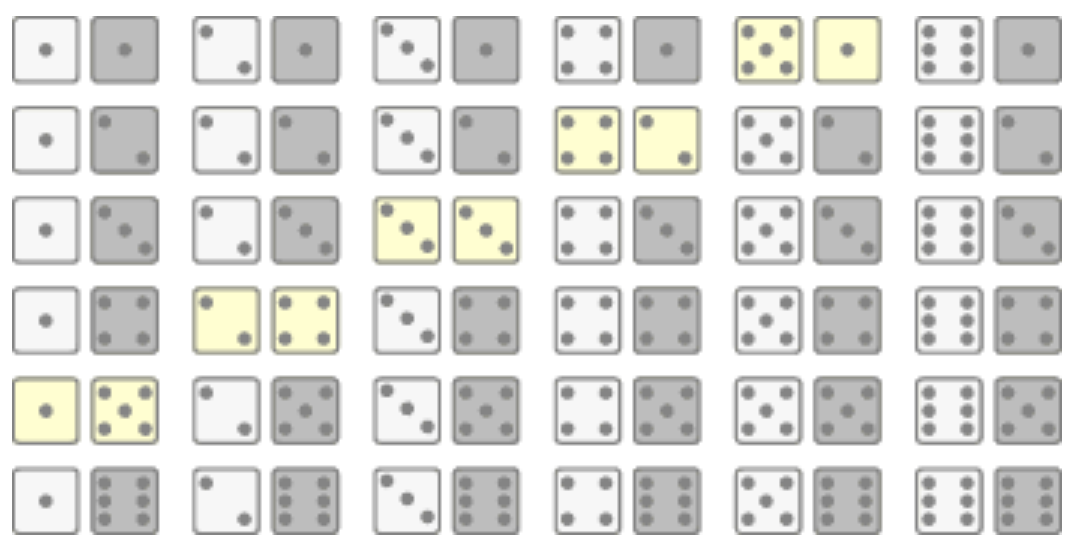
\includegraphics[width=0.5\linewidth]{topic01/sixSidedDice} 

}

\caption{Sample space of the experiment of rolling two dice.}\label{fig:unnamed-chunk-21}
\end{figure}

Since there are five ways to get a sum of 6, \(P(E) = 5/36 \approx 0.14\).

\hypertarget{general-addition-rule}{%
\section{General Addition Rule}\label{general-addition-rule}}

John Venn developed a great way to visualize sets. This visual is usually called the Venn diagram. Because events are sets of outcomes of an experiment, it works well to visualize probability as well.

Here's an example of a Venn diagram showing two disjoint outcomes, E and F.

\begin{Shaded}
\begin{Highlighting}[]
\NormalTok{knitr}\SpecialCharTok{::}\FunctionTok{include\_graphics}\NormalTok{(}\StringTok{"topic01/venn.png"}\NormalTok{)}
\end{Highlighting}
\end{Shaded}

\begin{figure}

{\centering 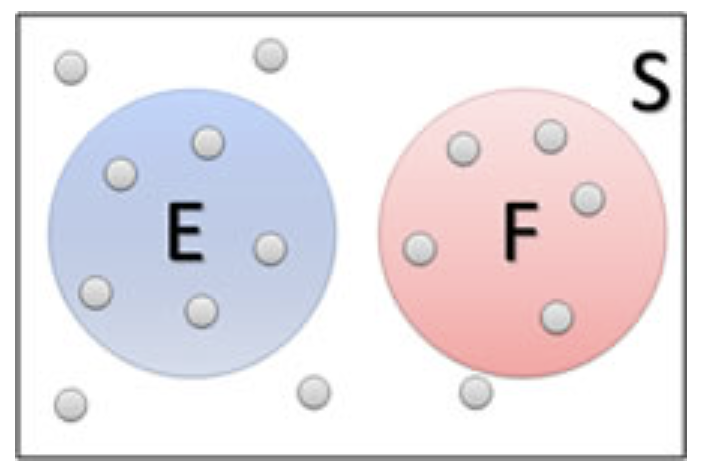
\includegraphics[width=0.3\linewidth]{topic01/venn} 

}

\caption{The Venn diagram of two events in a sample space.}\label{fig:unnamed-chunk-22}
\end{figure}

\hypertarget{additive-rule}{%
\subsection{Additive Rule}\label{additive-rule}}

Let E and F be defined in a sample space S of an experiment. The General Addition Rule is given by

\[P(E \mbox{ or } F) = P(E) + P(F) - P(E \mbox{ and } F)\]

The above general additive is depicted in the following Venn diagram

\begin{Shaded}
\begin{Highlighting}[]
\NormalTok{knitr}\SpecialCharTok{::}\FunctionTok{include\_graphics}\NormalTok{(}\StringTok{"topic01/additiveRule.png"}\NormalTok{)}
\end{Highlighting}
\end{Shaded}

\begin{figure}

{\centering 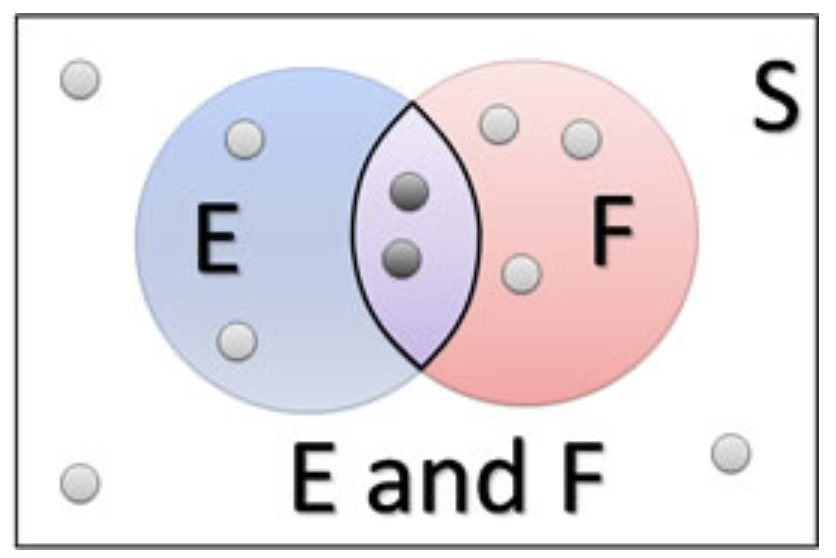
\includegraphics[width=0.3\linewidth]{topic01/additiveRule} 

}

\caption{Figure 3. Venn diagram representation of additive rule.}\label{fig:unnamed-chunk-23}
\end{figure}

\textbf{Example 4}: Consider a standard playing card. Suppose we draw one card at random from the deck and define the following events:

E = the card drawn is an ace

F = the card drawn is a king

Use these definitions to find P(E or F).

\begin{Shaded}
\begin{Highlighting}[]
\NormalTok{knitr}\SpecialCharTok{::}\FunctionTok{include\_graphics}\NormalTok{(}\StringTok{"topic01/classic{-}playing{-}cards{-}additive{-}rule.png"}\NormalTok{)}
\end{Highlighting}
\end{Shaded}

\begin{figure}

{\centering 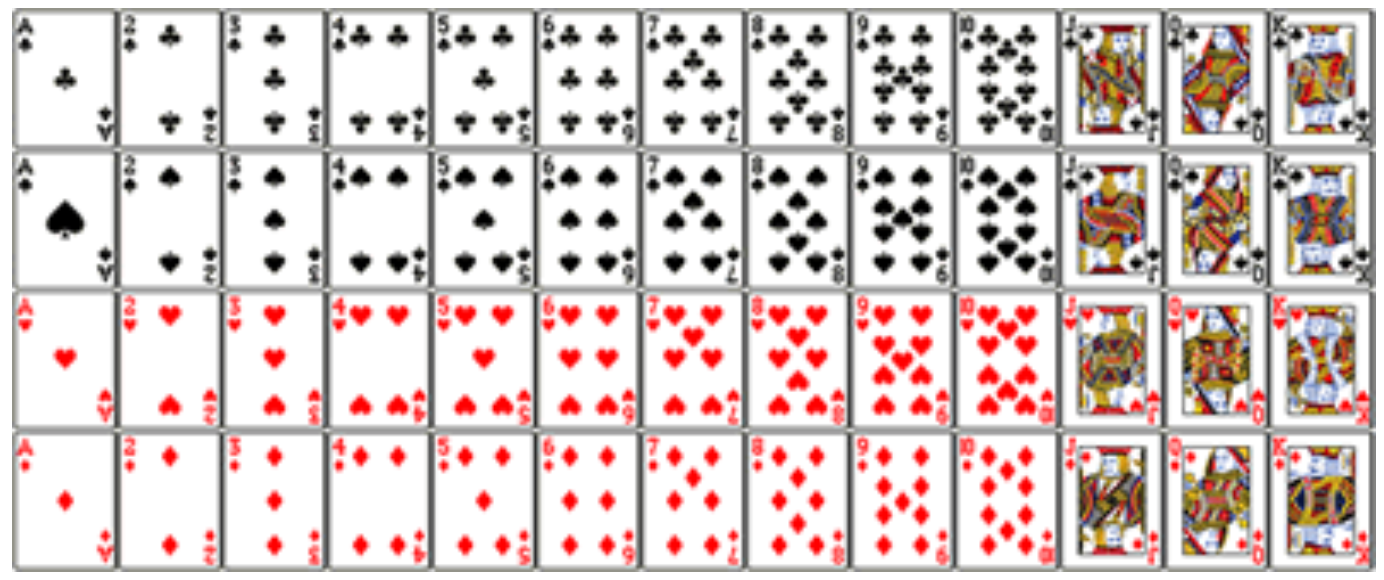
\includegraphics[width=0.6\linewidth]{topic01/classic-playing-cards-additive-rule} 

}

\caption{Additive rule - playing card example.}\label{fig:unnamed-chunk-24}
\end{figure}

\textbf{Solution}: Since E and F have no outcomes in common, we can use the Addition Rule for Disjoint Events:

\[P(E \mbox{ or } F) = P(E) + P(F) = 4/52 + 4/52 = 8/52 = 2/13.\]

\hypertarget{special-cases}{%
\subsection{Special Cases}\label{special-cases}}

\textbf{Case \#1}: If the two events are disjoint (mutually exclusive), the general additive rule is reduced to

\[P(E \mbox{ or } F) = P(E) + P(F)\]

\textbf{Example 5}: Suppose we have a family with three children, and we consider the sex of those three children. If we let B represent a boy and G represent a girl, here is the sample space:

\[S = \{ BBB, BBG, BGB, GBB, BGG, GBG, GGB, GGG\}\]

let's define the following events:

E = the family has exactly two boys

F = the family has exactly one boy

Describe the event \textbf{E or F} and find its probability.

\textbf{Solution}: \textbf{E or F} is the event that the family has either one or two boys.

Clearly, both of these events can't occur at the same time, so they are disjoint. The probability of the family having either one or two boys is then:

\[P(E \mbox{ or } F) = P(E) + P(F) = 3/8 + 3/8 = 6/8 = 3/4.\]

\textbf{Case \#2} - The Complement Rule.

The complement of E, denoted by \(E^c\), is all outcomes in the sample space that are not in E.

So essentially, the complement of E is everything but the outcomes in E. In fact, some texts actually write it as ``not E''. The following Venn diagram illustrates the event and its complement.

\begin{Shaded}
\begin{Highlighting}[]
\NormalTok{knitr}\SpecialCharTok{::}\FunctionTok{include\_graphics}\NormalTok{(}\StringTok{"topic01/complement.jpg"}\NormalTok{)}
\end{Highlighting}
\end{Shaded}

\begin{figure}

{\centering 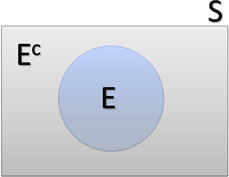
\includegraphics[width=0.3\linewidth]{topic01/complement} 

}

\caption{Complementary events.}\label{fig:unnamed-chunk-25}
\end{figure}

Since P(S) = 1. Clearly, E and \(E^c\) are disjoint, so \(P(E or E^c) = P(E) + P(E^c)\) . Combining those two facts, we get the following complementary Rule

\[P(E) + P(E^c) = 1\]

\hypertarget{multiplicative-rule-and-independence}{%
\section{Multiplicative Rule and Independence}\label{multiplicative-rule-and-independence}}

Two events E and F are \textbf{independent} if the occurrence of event E does not affect the probability of event F.

\textbf{Disjoint vs.~Independent}: It is very common for students to confuse the concepts of disjoint (mutually exclusive) events with independent events. Recall from the last section:

\begin{quote}
Two events are disjoint if they have no outcomes in common. (Also commonly known as mutually exclusive events.)
\end{quote}

\begin{Shaded}
\begin{Highlighting}[]
\NormalTok{knitr}\SpecialCharTok{::}\FunctionTok{include\_graphics}\NormalTok{(}\StringTok{"topic01/disjoint{-}indpemdent.jpg"}\NormalTok{)}
\end{Highlighting}
\end{Shaded}

\begin{figure}

{\centering 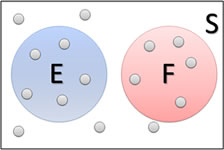
\includegraphics[width=0.3\linewidth]{topic01/disjoint-indpemdent} 

}

\caption{Disjoint and independent events.}\label{fig:unnamed-chunk-26}
\end{figure}

From the above figure, we can see very clearly that if event E occurs (that is, the outcome - gray circle- is in event E), it cannot possibly be in event F. So E and F are mutually exclusive.

\hypertarget{conditional-probability}{%
\subsection{Conditional Probability}\label{conditional-probability}}

The notation P(F\textbar E) is read \textbf{the probability of F given E} and represents the probability that event F occurs, given that event E has already occurred. Mathematically, the probability of F giving E is given by

\[P(F|E) = P(E \mbox{ and } F) / P(E)\]

\textbf{Example 6}: The following Venn diagram illustrates conditional probability.

\begin{Shaded}
\begin{Highlighting}[]
\NormalTok{knitr}\SpecialCharTok{::}\FunctionTok{include\_graphics}\NormalTok{(}\StringTok{"topic01/conditional.jpg"}\NormalTok{)}
\end{Highlighting}
\end{Shaded}

\begin{figure}

{\centering 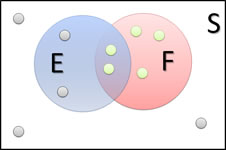
\includegraphics[width=0.3\linewidth]{topic01/conditional} 

}

\caption{Conditional probability.}\label{fig:unnamed-chunk-27}
\end{figure}

Based on the above Venn diagram, find P(E\textbar F).

\textbf{Solution}: P(E\textbar F) is the probability that event E occurs given that event F has already occurred. Let's change the image a bit. Since F has occurred, we can focus on just those \textbf{outcomes} in F. And then of those, we want the probability that the \textbf{outcome} is in E. Since there are 2 of those in E, and 5 total,

\[P(E|F) = P(E \mbox{ and } F) / P(F) = 2/5.\]

\hypertarget{general-multiplication-rule}{%
\subsection{General Multiplication Rule}\label{general-multiplication-rule}}

The probability that two events E and F both occur can be obtained from the definition of conditional probability in the following form

\[P(E \mbox{ and } F) = P(E) \times P(F|E)\]

The general multiplicative rule essentially expresses the joint probability as the product of a conditional probability and the probability of the conditioning event.

\textbf{Example 7}. Let's try a new probability experiment. This time, consider a bag of marbles, containing 10 red, 20 blue, and 15 green marbles. Suppose that two marbles are drawn without replacement. (The first marble is not put back in the bag before drawing the second.)

What is the probability that both marbles drawn are red?

\textbf{Solution}: Let's define a couple of events:

E = first marble is red

F = second marble is red

We want P(E and F). Using the General Multiplication Rule, we see

\[P(E \mbox{ and } F) = P(E)  \times P(F|E) = (10/45) \times (9/44) \approx 0.0455.\]

\hypertarget{checking-independence-using-multiplicative-rule}{%
\subsection{Checking Independence Using Multiplicative Rule}\label{checking-independence-using-multiplicative-rule}}

Two events E and F are independent if event E's occurrence does not affect event F's probability.

Looking at this in terms of conditional probability, if the occurrence of E doesn't affect the probability of F, then P(F\textbar E) = P(F). This is a good way to test for independence. In fact, we can redefine independence using this concept.

Two events E and F are independent if P(F\textbar E) = P(F).

\textbf{Example 8}: Consider a survey given to 52 students in an introductory statistics class, with the following responses to the statement \textbf{I enjoy statistics.}

\begin{Shaded}
\begin{Highlighting}[]
\NormalTok{knitr}\SpecialCharTok{::}\FunctionTok{include\_graphics}\NormalTok{(}\StringTok{"topic01/checkingIndep.png"}\NormalTok{)}
\end{Highlighting}
\end{Shaded}

\begin{center}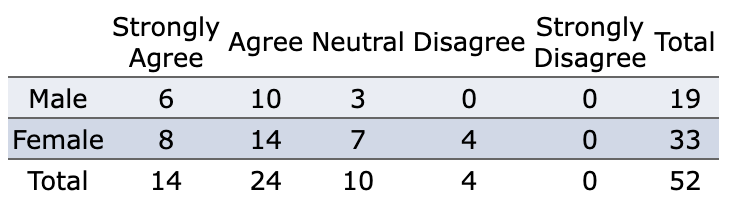
\includegraphics[width=0.45\linewidth]{topic01/checkingIndep} \end{center}

Suppose a student is selected at random from those surveyed and we define the events E and F as follows:

E = student selected is female

F = student enjoys math

Are events E and F independent?

\textbf{Solution}: To answer this, we'll need to see if P(F\textbar E) = P(F).

\(P(F) = 38/52 \approx 0.7308\)

\(P(F|E) = 22/33 \approx 0.6667\)

Since \(P(F) \ne P(F|E)\), events E and F are dependent.

\hypertarget{bayes-theorem}{%
\subsection{Bayes' Theorem}\label{bayes-theorem}}

Bayes' Theorem (also called Bayes Rule) is a way of finding a (posterior) probability when we know certain other (prior) probabilities.

The formula is:

\[P(A|B) =  P(A) \times P(B|A) = P(B)\]

\textbf{Which tells us}: how often A happens given that B happens, written P(A\textbar B),

\textbf{When we know}:\\
* how often B happens given that A happens, written P(B\textbar A)
* how likely A is on its own, written P(A)
* how likely B is on its own, written P(B)

Let us say P(Fire) means how often there is fire, and P(Smoke) means how often we see smoke, then:

P(Fire\textbar Smoke) means how often there is fire when we can see smoke;

P(Smoke\textbar Fire) means how often we can see smoke when there is fire

So the formula basically tells us \textbf{forward} P(Fire\textbar Smoke) when we know \textbf{backward} P(Smoke\textbar Fire)

\hfill\break

\textbf{Example 9}: Picnic Day - Suppose we are planning a picnic today, but the morning is cloudy.

Given the following prior information:

\begin{itemize}
\tightlist
\item
  50\% of all rainy days start off cloudy!
\item
  But cloudy mornings are common (about 40\% of days start cloudy)
\item
  And this is usually a dry month (only 3 of 30 days tend to be rainy, or 10\%)
\end{itemize}

What is the chance of rain during the day?

\textbf{Solution}: We will use Rain to mean rain during the day, and Cloud to mean cloudy morning.

The chance of Rain given Cloud is written P(Rain\textbar Cloud)

So let's put that in the formula:

P(Rain\textbar Cloud) = P(Rain) P(Cloud\textbar Rain) / P(Cloud)

P(Rain) is Probability of Rain = 10\%

P(Cloud\textbar Rain) is the Probability of Cloud, given that Rain happens = 50\%

P(Cloud) is Probability of Cloud = 40\%

\(P(Rain|Cloud) = 0.1 \times 0.5 /0.4 = .125\)

Or a 12.5\% chance of rain. Not too bad, let's have a picnic!

One of the famous uses for the Bayes Theorem is \textbf{False Positives and False Negatives}.

We use PCR test result of COVID-19 as an example to explain

\textbf{False Positives} = A person's PCR is positive but was not infected with COVID-19.

\textbf{False Negatives} = A person's PCR is negative but was infected with COVID-19.

\hfill\break

\textbf{Example 9}: Allergy or Not? - Hunter says she is itchy. There is a test for Allergy to Cats, but this test is not always right:

\begin{itemize}
\item
  For people that really do have the allergy, the test says \textbf{Yes} 80\% of the time
\item
  For people that do not have the allergy, the test says \textbf{Yes} 10\% of the time (\textbf{false positive})
\item
  If 1\% of the population has the allergy, and Hunter's test says \textbf{Yes}, what are the chances that Hunter really has the allergy?
\end{itemize}

We want to know the chance of having the allergy when the test says \textbf{Yes}, written P(Allergy\textbar Yes)

\textbf{Solution}: Let's get our formula:

P(Allergy\textbar Yes) = P(Allergy) P(Yes\textbar Allergy) / P(Yes)

P(Allergy) is Probability of Allergy = 1\%

P(Yes\textbar Allergy) is the probability of the test saying \textbf{Yes} for people with allergy = 80\%

We need to find P(Yes) is the probability of the test saying \textbf{Yes} (to anyone) = ??\%

We can calculate it by adding up those with, and those without the allergy:

\begin{itemize}
\item
  1\% have the allergy, and the test says \textbf{Yes} to 80\% of them
\item
  99\% do not have the allergy and the test says \textbf{Yes} to 10\% of them
\end{itemize}

Then \(P(Yes) = 1\% \times 80\% + 99\% \times 10\% = 10.7\%\), which means that about 10.7\% of the population will get a \textbf{Yes} result. Therefore,

\[P(Allergy|Yes) =  1\% \times 80\% / 10.7\% = 7.48\%\]

That is, \(P(Allergy|Yes) \approx 7\%\).

\hfill\break

\hfill\break

\textbf{Acknowledgment}

'The content of this note is based on \url{https://faculty.elgin.edu/dkernler/statistics/ch05/}

\hfill\break

\hfill\break

\hypertarget{appendix-calculus-review-topics}{%
\section{Appendix: Calculus Review Topics}\label{appendix-calculus-review-topics}}

This appendix reviews the basics of single variable functions.

\hypertarget{notation-domain-and-range}{%
\subsection{Notation, Domain, and Range}\label{notation-domain-and-range}}

\begin{itemize}
\tightlist
\item
  \textbf{Notation}: Functions can also be written in the form of \(f(x)\), pronounced \textbf{f of x}. When someone says \textbf{y is a function of x}, it means that the value of y is determined by the value of x. Here, y is the dependent variable and x is the independent variable. \(f(x)\) is just the shortened form of \textbf{function of x}.
\end{itemize}

\textbf{Example 10}: A function can be denoted in different forms. The following are the two forms of the same function.

\[
y = x^2 + 2 \mbox{   and   } f(x) = x^2 + 2\]

\begin{itemize}
\item
  \textbf{Domain}: The domain of a function is all the possible values of the independent variable, \(x\), for which \(y\) is defined.
\item
  \textbf{Range}: The range of a function is all the possible values of the dependent variable \(y\).
\end{itemize}

\textbf{Example 11}: The given function \(f(x) = x^2\) has a domain of all real numbers (\(x\) can be anything) and a range that is greater than or equal to zero.

\hypertarget{operations-of-functions}{%
\subsection{Operations of Functions}\label{operations-of-functions}}

We can define new functions based on the existing functions using basic arithmetic operations.

\textbf{Example 12} Let \(f(x) = x^2 + 1\) and \(g(x) = \sqrt{x+1}\). We can define the following new functions.

\begin{itemize}
\item
  \(h_1(x) = f(x) + g(x) = x^2 + \sqrt{x+1} + 1\).
\item
  \(h_2(x) = f(x) - g(x) = x^2 + 1 -\sqrt{x+1}\).
\item
  \(h_3(x) = f(x)\times g(x) = (x^2 + 1)\times \sqrt{x+1}\).
\item
  \(h_4(x) = f(x) / g(x) = (x^2 + 1)/\sqrt{x+1}\).
\end{itemize}

\hypertarget{composite-functions}{%
\subsection{Composite Functions}\label{composite-functions}}

A \textbf{composite function} is a function created when one function is used as the input value for another function. Essentially, the output of the inner function (the function used as the input value) becomes the input of the outer function (the resulting value).

\begin{itemize}
\tightlist
\item
  \textbf{Notation}: For the functions \(f(x)\) and \(g(x)\), when \(g(x)\) is used as the \textbf{input} of \(f(x)\), the composite function is written as:
\end{itemize}

\[(f \circ g)(x)\]

The \(\circ\) symbol denotes a composite function - it looks similar to the multiplication symbol, \(\cdot\), but does not mean the same thing. \((f \circ g)(x)\) is the same thing as \(f(g(x))\).

\((f \circ g)(x)\) is not the same thing as \((g \circ f)(x)\). \((g \circ f)(x)\) is the same thing as \(g(f(x))\), which will often be different than \(f(g(x))\).

You can use composite functions to check if two functions are inverses of each other because they will follow the rule:

\[(f \circ g)(x) = (g \circ f)(x) = x\]

We can find the composite of two functions by replacing every \(x\) in the outer function with the equation for the inner function (the input).

\textbf{Example 13}: Given: \(f(x) = 4x2 + 3\) and \(g(x) = 2x + 1\).

\[(f \circ g)(x)    =   f(g(x)) = 4(2x + 1)^2 + 3
    =   4(4x^2 + 4x + 1) + 3
    =   16x^2 + 16x + 7\]

\[(g \circ f)(x)    =   g(f(x)) = 2(4x^2 + 3) + 1   =   8x^2 + 6 + 1\]

\hypertarget{inverse-function}{%
\subsection{Inverse Function}\label{inverse-function}}

Inverse functions are a way to ``undo'' a function. In the original function, plugging in \(x\) gives back \(y\), but in the inverse function, plugging in \(y\) (as the input) gives back \(x\) (as the output). If a function were to contain the point (3,5), its inverse would contain the point (5,3).

If the original function is \(f(x)\), then its inverse \(f^{-1}(x)\) is \textbf{not the same as} \(1/f(x)\) .

To find the inverse of a function, we need to do the opposite of what the original function does to \(x\). To be more specific, we can use the following steps:

\begin{enumerate}
\def\labelenumi{\arabic{enumi}.}
\item
  In the original equation, replace \(f(x)\) with \(y\);
\item
  Replace every \(x\) in the original equation with a \(y\) and every \(y\) in the original equation with an \(x\);
\item
  Solve for \(y\);
\item
  Change \(y\) to \(f^{-1}(x)\);
\end{enumerate}

\hfill\break

\textbf{Example 14}: Find the inverse function of \(f(x) = 5\sqrt{x+4}-3\).

\textbf{Solution}. We follow the above steps to find the inverse function.

\begin{Shaded}
\begin{Highlighting}[]
\NormalTok{knitr}\SpecialCharTok{::}\FunctionTok{include\_graphics}\NormalTok{(}\StringTok{"topic01/inverseFun.png"}\NormalTok{)}
\end{Highlighting}
\end{Shaded}

\begin{center}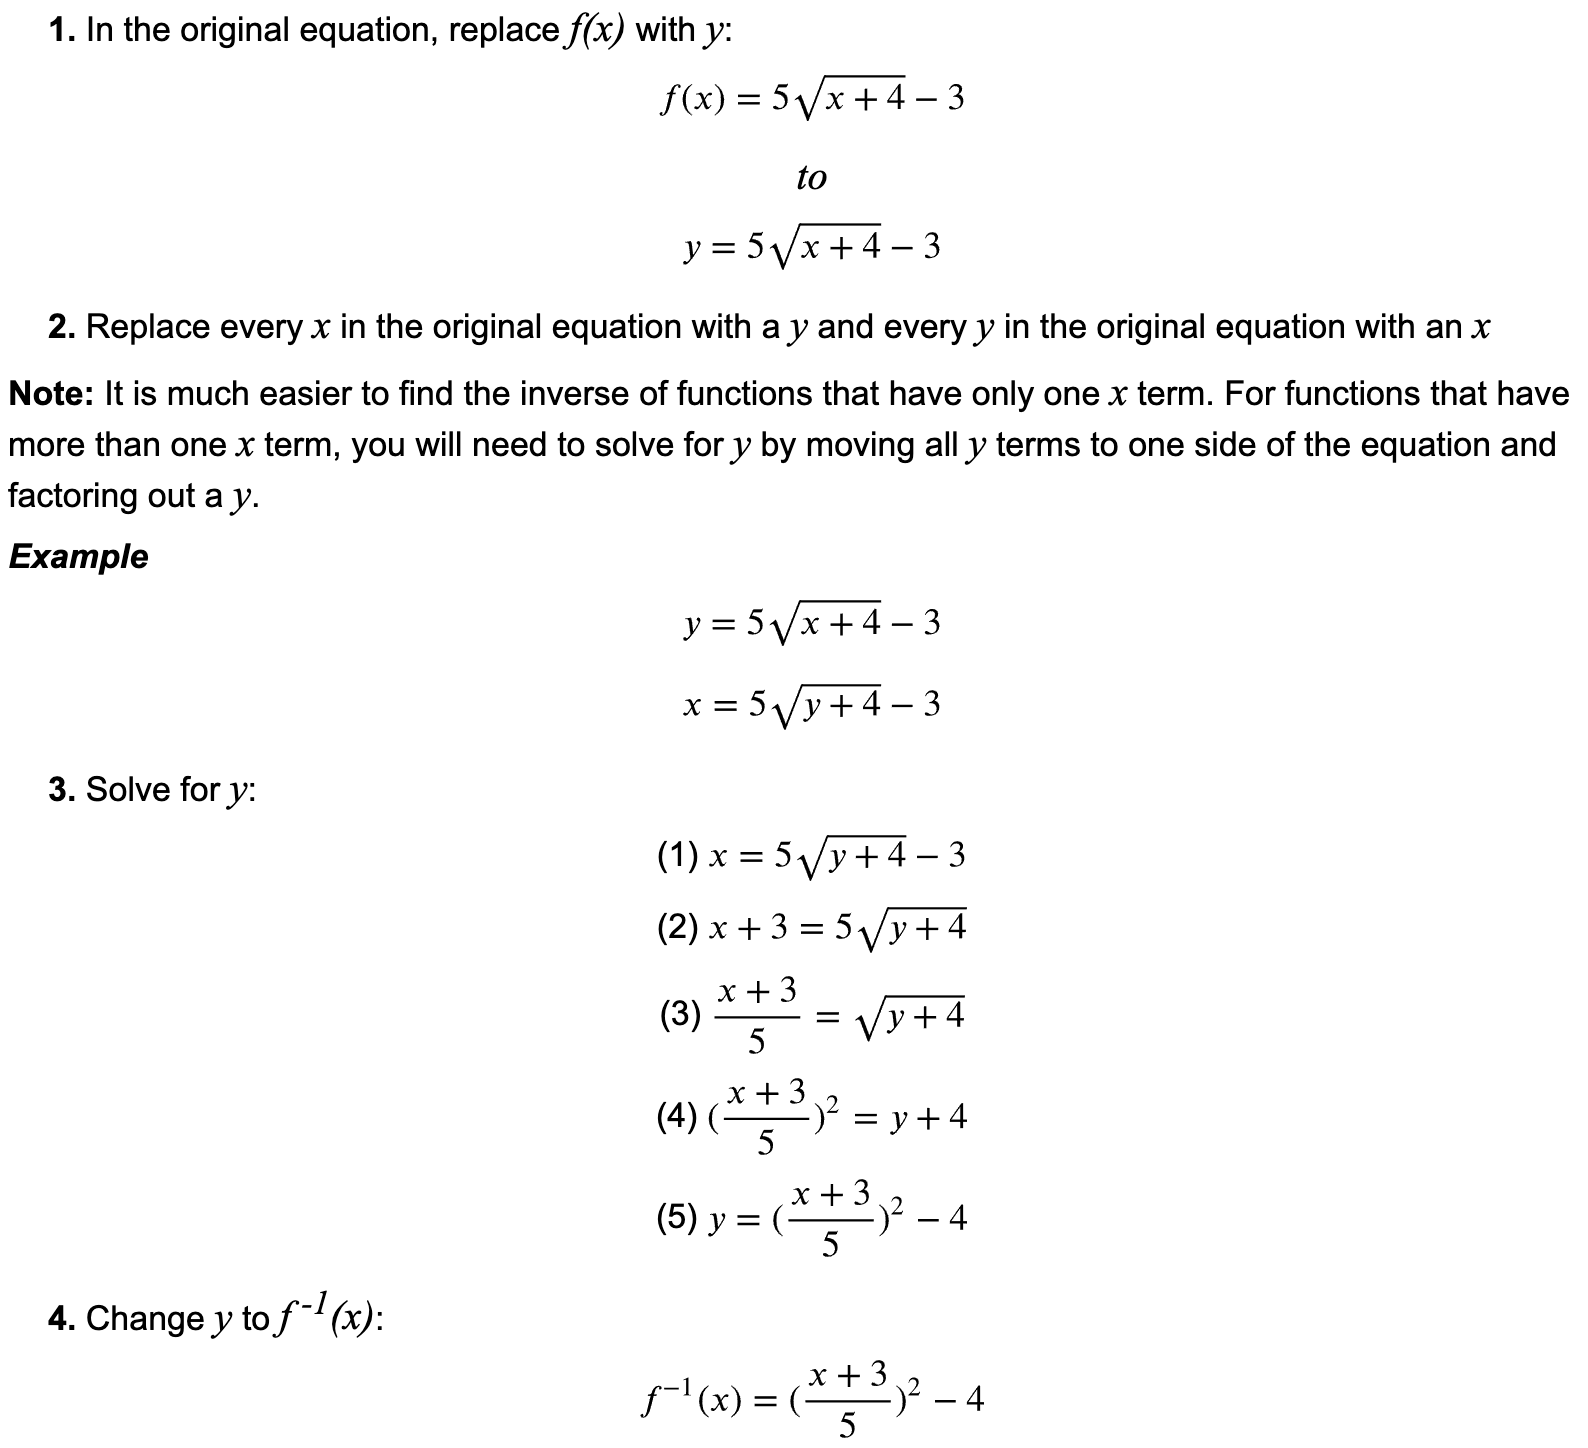
\includegraphics[width=0.8\linewidth]{topic01/inverseFun} \end{center}

\hfill\break

\hypertarget{practice-exercises}{%
\subsection{Practice Exercises}\label{practice-exercises}}

The following link \url{https://github.com/pengdsci/WCUSTA504/raw/main/topic01/FunctionsWorksheet.pdf} gives a list of exercises that reflect the concepts reviewed in this appendix.

\hfill\break

\hypertarget{discrete-random-variables-and-their-distribution}{%
\chapter{Discrete Random Variables and Their Distribution}\label{discrete-random-variables-and-their-distribution}}

\emph{(Relevant contents in the textbook: Section 3.1)}

A \textbf{random variable} is a real-valued function defined on the sample space S. Probabilities are assigned to the possible values of the random variable. In other words, suppose Y is a random variable. Then

\begin{itemize}
\tightlist
\item
  Y takes on real numbers as values, i.e., \(Y\in R\).
\item
  \(P(Y\in B)\) is defined for any \textbf{measurable} set B of real numbers.
\end{itemize}

\textbf{Example 1}: Examples of random variables

\begin{enumerate}
\def\labelenumi{\arabic{enumi}.}
\item
  Y = the sum of the two numbers that come up on tossing two dice.
\item
  Y = the amount of annual precipitation in inches for Portland.
\item
  Y = the number of students who will enroll in Math 282 after taking this class.
\end{enumerate}

\textbf{Example 2}: \emph{Coin Toss experiment}. Assuming a fair coin, let Y = 1 for a head, and Y = 0 for a tail. Then \(P(Y=1) = P(Y=0) = 0.5\).

Note: \(P(Y = 2) = 0\) In fact, \(P(Y \notin \{0, 1 \}) = 0\).

\textbf{Example 3}: Number of Boys in a family with three children.

\textbf{Random sampling} is a method of sampling in which every possible sample of \(n\) elements to be sampled has an equal probability of being selected.

\hypertarget{characterization-of-distribution-of-random-variables}{%
\section{Characterization of Distribution of Random Variables}\label{characterization-of-distribution-of-random-variables}}

\emph{(Textbook: Sections 3.2 and 3.3)}

\textbf{Discrete random variables} take on only a finite or countably infinite number of distinct values.

\textbf{The probability distribution of a random variable} provides information (using a formula, a table, or a graph) about the probability that a random value takes on each one of its possible values.

\hypertarget{definition-of-rv}{%
\subsection{Definition of RV}\label{definition-of-rv}}

Let Y be a random variable, and \(p(y) = P(Y =y)\), the probability of \(Y\) taking value \(y\). Suppose that Y takes the values \(\{ y_1, y_2, \cdots, y_k\}\) where k may be \(\infty\). If both of the following conditions are satisfied,

\begin{enumerate}
\def\labelenumi{\arabic{enumi}.}
\item
  \(0 \le P(Y = y_i) \le 1\)
\item
  \(\sum_{i=1}^k P(Y=y_i) = 1\).
\end{enumerate}

\(p(y) = P(Y =y)\) is called the probability distribution of random variable \(Y\). \texttt{Note\ that\ \$P(Y\ =\ y)\$\ could\ have\ an\ explicit\ expression\ in\ the\ form\ of\ a\ non-negative\ function.}

\textbf{Example 4}: Toss a fair coin three times. Let Y denote the number of heads appearing. Note that Y can take on only four values: 0, 1, 2, and 3. Then

\(P(0) = P(Y = 0) = P(\{ TTT\}) = 1/8\)

\(P(1) = P(Y = 1) = P(\{ HTT, THT, TTH\}) = 3/8\)

\(P(2) = P(Y = 2) = P(\{ HHT, HTH, THH\}) = 3/8\)

\(P(3) = P(Y = 3) = P(\{ HHH\}) = 1/8\)

We will revisit this example and provide a formula for \(P(Y = y)\) for this example later.

\hypertarget{expectation-and-variance}{%
\subsection{Expectation and Variance}\label{expectation-and-variance}}

Let \(Y\) be a discrete random variable.

\begin{enumerate}
\def\labelenumi{\arabic{enumi}.}
\item
  The expectation or the expected value or the mean of Y is defined as \(\mu = E[Y] =\sum_y yp(y)\),
  where the index \(y\) in the summation is for all possible values of \(Y\).
\item
  The \textbf{expected value} of a function of Y, \(g(Y)\), is given by \(E[g(Y)] =\sum_y g(y)p(y)\).
\item
  The \textbf{variance} of a random variable Y is given by \(\sigma^2 = V[Y] = E[(Y-\mu)^2]\), where \(\mu = E[Y]\).
\end{enumerate}

\textbf{Comment}: \emph{An expectation of a random variable (or a function of a random variable) is simply the weighted average of the values (taking taken by the random variable/the function of the random variable). The weights are corresponding probability of \(Y\) taking its distinct values}.

\textbf{Example 5}: (use the experiment and the random variable in \textbf{example 4}).

\[\mu = E[X]  = 0\times 1/8 + 1\times (3/8) + 2\times (3/8) + 3\times (1/8)= 3(1+2+1)/8 = 3/2.\]

\[\sigma^2 = E[(X-\mu)^2]  = (0-1.5)^2\times (1/8) +(1-1.5)^2\times (3/8) + (2-1.5)^2\times (3/8) + (3-1.5)^2\times (1/8) = 0.75.\]

\textbf{Note}: In the above example, \((X-\mu)^2\) is considered as a function of random variable \(Y\).

\hypertarget{some-properties-of-expectation-and-variance}{%
\subsection{Some Properties of Expectation and Variance}\label{some-properties-of-expectation-and-variance}}

Let c be a constant and \(g(Y), g_1(Y)\) and \(g_2(Y)\) be functions of random variable Y. Then

\begin{enumerate}
\def\labelenumi{\arabic{enumi}.}
\item
  \(E[c] = c.\)
\item
  \(E[cg(Y)] = cE[g(Y)]\)
\item
  \(E[g_1(Y) + g_2(Y)] = E[g_1(Y)] + E[g_2(Y)]\)
\item
  \(\sigma^2 = V[Y] = E[(Y-\mu)^2] = E(Y^2) - \mu^2.\)
\end{enumerate}

\textbf{Proof}: The proofs are not difficult. You need to use the definition of the expectation to complete the these proof. You can find details from your textbook.

\textbf{Example 6}: Roll two fair six-sided dice. Let X = sum of the outcomes of the dice. Find

A). E{[}X{]}

B). E{[}\(X^2\){]}

C). Var(X)

\textbf{Solution} The above quantities can be calculated based on the following sample space.

\begin{Shaded}
\begin{Highlighting}[]
\NormalTok{knitr}\SpecialCharTok{::}\FunctionTok{include\_graphics}\NormalTok{(}\StringTok{"topic02/tossCoin2SampleSpace.png"}\NormalTok{)}
\end{Highlighting}
\end{Shaded}

\begin{center}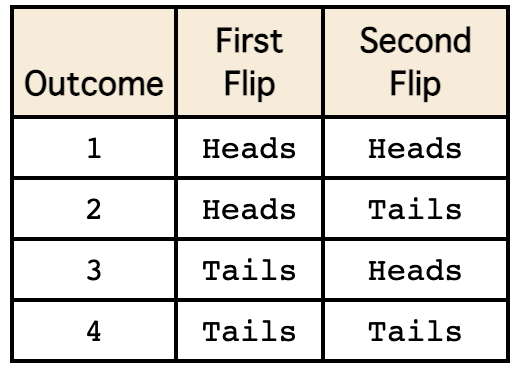
\includegraphics[width=0.3\linewidth]{topic02/tossCoin2SampleSpace} \end{center}

and the following probability distribution table.

\begin{Shaded}
\begin{Highlighting}[]
\NormalTok{knitr}\SpecialCharTok{::}\FunctionTok{include\_graphics}\NormalTok{(}\StringTok{"topic02/tossCoin2ProbDist.png"}\NormalTok{)}
\end{Highlighting}
\end{Shaded}

\begin{center}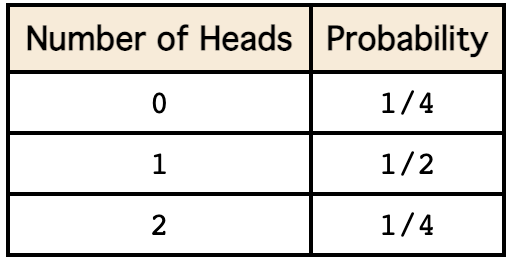
\includegraphics[width=0.3\linewidth]{topic02/tossCoin2ProbDist} \end{center}

\hypertarget{characterization-of-a-random-variable}{%
\subsection{Characterization of A Random Variable}\label{characterization-of-a-random-variable}}

To study the random behavior of a random variable, we need to follow the following three steps.

\textbf{Three-step Characterization Procedure}

\begin{enumerate}
\def\labelenumi{\arabic{enumi}.}
\item
  Clearly define the random variable associated with the (random experiment).
\item
  Define the probability distribution of the random variable.
\item
  Calculation of moment (i.e., the expectation of the power of the random variable)
\end{enumerate}

\textbf{Example 7}: We define a random variable based on an experiment of tossing three fair coins.

We follow the above three steps to define and characterize a random variable.

\texttt{Step\ 1}. Define \$X = \$ number of heads observed in an experiment of tossing a coin three times.

\texttt{Step\ 2}. The distribution of \(X\) is characterized in the following table using the sample size

\[S=\{HHH, HHT, HTH, THH, TTT, TTH, THT, HTT \}\]

\begin{Shaded}
\begin{Highlighting}[]
\NormalTok{knitr}\SpecialCharTok{::}\FunctionTok{include\_graphics}\NormalTok{(}\StringTok{"topic02/SampleSpace.png"}\NormalTok{)}
\end{Highlighting}
\end{Shaded}

\begin{center}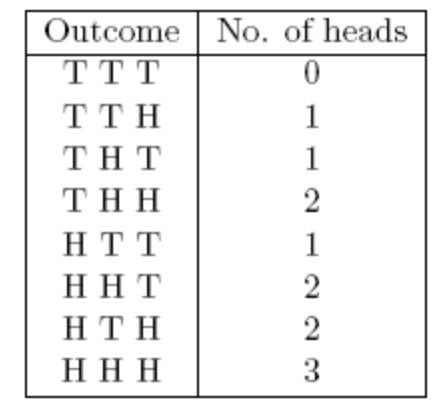
\includegraphics[width=0.3\linewidth]{topic02/SampleSpace} \end{center}

The \textbf{probability distribution table} is given by

\begin{Shaded}
\begin{Highlighting}[]
\NormalTok{knitr}\SpecialCharTok{::}\FunctionTok{include\_graphics}\NormalTok{(}\StringTok{"topic02/DistTable.png"}\NormalTok{)}
\end{Highlighting}
\end{Shaded}

\begin{center}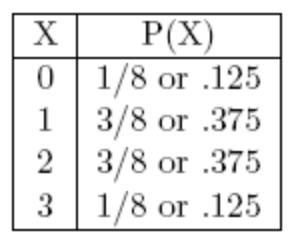
\includegraphics[width=0.3\linewidth]{topic02/DistTable} \end{center}

This distribution can also be defined using the following \textbf{probability distribution histogram}

\begin{Shaded}
\begin{Highlighting}[]
\NormalTok{knitr}\SpecialCharTok{::}\FunctionTok{include\_graphics}\NormalTok{(}\StringTok{"topic02/DistHist.png"}\NormalTok{)}
\end{Highlighting}
\end{Shaded}

\begin{center}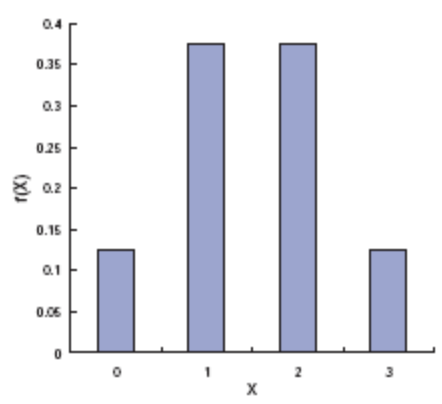
\includegraphics[width=0.3\linewidth]{topic02/DistHist} \end{center}

Another way to define this distribution is to use a formula (also called \textbf{probability distribution function}).
\[
\displaystyle f(x) = \begin{cases} 
 1/8 & \text{if $x = 0,3$} \\  
 3/8 & \text{if $x = 1,2.$}  
 \end{cases}
\]
\texttt{Step\ 3}. The k-th moment is defined to be

\[\mu_k = E[X^k] = 0^k P(X=0) + 1^k P(X=1) + 2^k P(X=2) + 3^k P(X = 3) = 3/8 + 2^k (3/8) + 3^k (1/8) = 3(1+2^k+3^{k-1})/8.\]
Some special cases:

\begin{itemize}
\tightlist
\item
  \(\mu = E[X] = 3(1 +2^1 +3^{1-1})/8 = 3\times 4 /8 = 1.5\).
\item
  \(\sigma^2 = E[X^2] - \mu^2 = 3(1+2^2 +3^{2-1})/8 - 1.5^2 = 3\times 8/8 - 2.25 = 3-2.25 = 0.75.\)
\end{itemize}

\hypertarget{special-discrete-distributions}{%
\section{Special Discrete Distributions}\label{special-discrete-distributions}}

There are many well-known discrete random variables. The textbook introduces binomial, geometric, hypergeometric, negative binomial, and Poisson distributions. In this section, we choose the two most commonly used ones as examples to illustrate how to characterize discrete random variables.

\hypertarget{binomial-distribution}{%
\subsection{Binomial Distribution}\label{binomial-distribution}}

\emph{(Textbook: Section 3.4)}

The binomial distribution is one of the key distributions for several generalized linear models to be covered in subsequent courses.

Suppose there are \(n\) identical and independent binary trials, each with a success probability \(p\) (and failure probability \(1-p\)). Let \(Y\) be the number of successes in \(n\) trials. Then \(Y\) is called a binomial random variable. Its probability distribution is called binomial distribution accordingly.

The probability distribution of \(Y\) is given by

\[
P(Y = y) = \frac{n!}{y!(n-y)!}p^y(1-p)^{n-y} = {n\choose y}p^y(1-p)^{n-y}
\]
where \(y = 0, 1, \cdots, n\).

Note that there difference ways to denote \textbf{choosing y from n} in mathematics. For example

\[
{n\choose y}, \mbox{   } C_n^y, \mbox{   }  Cy^n,  \mbox{   }  _nCy,  \mbox{   }  C_{n,y}
\]

Since binomial distribution is a special discrete distribution, we can derive the following formulas of \textbf{expectation} and \textbf{variance} after some algebra.

\[\mu = E[Y] = np \hspace{3mm}\mbox{ and } \hspace{3mm}\sigma^2 = V[Y] = np(1-p)\]

Our textbook proves the above two formulas.

\textbf{Properties of binomial random variable}

\begin{enumerate}
\def\labelenumi{\arabic{enumi}.}
\item
  The experiment consists of n identical trials.
\item
  Each trial results in one of two outcomes often referred to as success (S) and failure (F).
\item
  The probability of success on a single trial is denoted by p and remains constant from trial to trial. The probability of failure is often denoted by \(q = 1 – p\).
\item
  The outcomes of the trials are independent.
\item
  The random variable that results from this random experiment is Y = the number of successes in the n trials.
\end{enumerate}

These 5 properties are used to justify whether a random variable is a binomial random variable.

\textbf{Example 8}: Assuming that about 85\% of students in a particular Statistics course are successful. Suppose 20 students are selected at random from all previous students in this course. What is the probability that 15 of them will have been successful in the course?

\textbf{Solution}: We first check the criteria for a binomial experiment to see if this fits.

\begin{itemize}
\tightlist
\item
  A fixed number of trials - The students are our trials.
\item
  Each trial is independent of the others - Since they're randomly selected, we can assume they are independent of each other.
\item
  There are only two outcomes - Each student either was successful or was not successful.
\item
  The probability of each outcome remains constant from trial to trial. - Because the students were independent, we can assume this probability is constant.
\end{itemize}

If we let X = the number of students who were successful, it does look like X follows the binomial distribution. For this example, \(n = 20\) and \(p = 0.70\). Therefore,

\[
P(X=15) = \frac{20!}{5!15!} 0.7^{15} 0.3^5 =  0.1789.
\]

We can use \textbf{R functions} to find relevant quantities related to the binomial distribution.

\begin{verbatim}
dbinom(x, size, prob, log = FALSE)
pbinom(q, size, prob, lower.tail = TRUE, log.p = FALSE)
qbinom(p, size, prob, lower.tail = TRUE, log.p = FALSE)
rbinom(n, size, prob)
\end{verbatim}

\hypertarget{poisson-distribution}{%
\subsection{Poisson Distribution}\label{poisson-distribution}}

\emph{(Textbook: Section 3.8)}

\begin{itemize}
\tightlist
\item
  \textbf{The Poisson Probability Distribution}.
\end{itemize}

If Y is the random variable representing `the number of occurrences in a given interval' for which the average rate of occurrences is \(\lambda\), then Y is called a Poisson random variable.

\textbf{Example 9}: Real-world phenomena for which the Poisson distribution provides a reasonable probability model:

\begin{enumerate}
\def\labelenumi{\arabic{enumi}.}
\tightlist
\item
  The number of accidents at an intersection in a month
\item
  The number of typographical errors on a page in a book
\item
  The number of emitted particles from radioactive material in a fixed period of time
\end{enumerate}

\begin{itemize}
\tightlist
\item
  \textbf{The Use of Poisson Distribution}
\end{itemize}

\textbf{Poisson distributions} can be used to model these situations because there are many ``trials'' and the probability of the event of interest occurring is small. For example, the large number of cars passing through an intersection in a year can be considered many ``trials'' and the probability of any car having an accident p is small.

\begin{itemize}
\tightlist
\item
  \textbf{Requirements of Poisson Distribution}
\end{itemize}

\begin{enumerate}
\def\labelenumi{\arabic{enumi}.}
\tightlist
\item
  The random variable X is the number of occurrences of an event over a specified interval. The interval could be time, distance, area, volume, etc.
\item
  The occurrences must be random.
\item
  The occurrences must be independent of each other.
\item
  The occurrences must be uniformly distributed over the interval being used.
\end{enumerate}

\begin{itemize}
\tightlist
\item
  \textbf{Properties of Poisson Distribution}
\end{itemize}

Let \(Y\) be the Poisson random variable with mean \(\lambda\).

\begin{enumerate}
\def\labelenumi{\arabic{enumi}.}
\tightlist
\item
  The distribution is given by
\end{enumerate}

\[
 P(Y=y) = \frac{\lambda^y e^{-y}}{y!}
 \]

where y = 0, 1, 2, \ldots., and

\begin{enumerate}
\def\labelenumi{\arabic{enumi}.}
\setcounter{enumi}{1}
\tightlist
\item
  The mean and the variance are
\end{enumerate}

\[ E[Y] = V[Y] = \lambda \]
\textbf{Proof}: It is easy to prove that the above expression gives a probability distribution based on the following identity

\begin{itemize}
\tightlist
\item
  \textbf{R Functions for Poisson Distribution}
\end{itemize}

The following four functions are associated with Poisson distributions.

\begin{verbatim}
dpois(x, lambda, log = FALSE)
ppois(q, lambda, lower.tail = TRUE, log.p = FALSE)
qpois(p, lambda, lower.tail = TRUE, log.p = FALSE)
rpois(n, lambda)
\end{verbatim}

\hypertarget{cumulative-distributions}{%
\section{Cumulative Distributions}\label{cumulative-distributions}}

\emph{(Textbook: mentioned in Section 4.2)}

Given a probability density function, we define the cumulative distribution function (CDF) as follows.

\hypertarget{definition-and-notations}{%
\subsection{Definition and Notations}\label{definition-and-notations}}

The cumulative distribution function (CDF) of a random variable X is denoted by \(F(x)\), and is defined as \(F(x) = P(X \le x)\). Using our identity for the probability of disjoint events, if X is a discrete random variable, we can write

\[
F(x) = \sum_{k=1}^n P(X = x_k)
\]

where \(x_n\) is the largest possible value of \(X\) that is less than or equal to \(x\).

In other words, the cumulative distribution function for a random variable at x gives the probability that the random variable X is less than or equal to that number x. Note that in the formula for CDFs of discrete random variables, we always have \(n \le N\), where \(N\) is the number of possible outcomes of \(X\).

Notice also that the CDF of a discrete random variable will remain constant on any interval of the form \([x_{n-1}, x_n]\). That is,

\[
F(x) = F(x_{n-1}) = \sum_{k=1}^{n-1} P(X = x_n)
\]
for any \(x\in [x_{n-1}, x_n]\).

\textbf{Example 10}: Suppose that we have two fair six-sided dice, one yellow and one red as in the image below.

\begin{Shaded}
\begin{Highlighting}[]
\NormalTok{knitr}\SpecialCharTok{::}\FunctionTok{include\_graphics}\NormalTok{(}\StringTok{"topic02/TwoDice.jpg"}\NormalTok{)}
\end{Highlighting}
\end{Shaded}

\begin{center}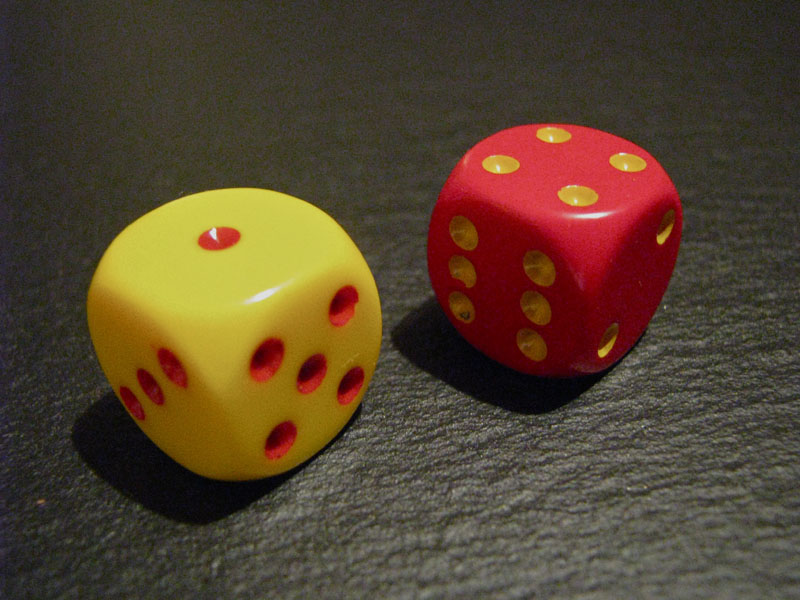
\includegraphics[width=0.3\linewidth]{topic02/TwoDice} \end{center}

We roll both dice at the same time and add the two numbers that are shown on the upward faces.
Let \(X\) be the discrete random variable associated with this sum.

\begin{enumerate}
\def\labelenumi{\arabic{enumi}.}
\item
  How many possible outcomes are there? That is, how many different values can \(X\) assume?
\item
  How is X distributed? That is, what is the PDF of \(X\)?
\item
  What is the CDF of \(X\)?
\item
  What is the probability that \(X\) is less than or equal to 6?
\end{enumerate}

\textbf{Solution}

\begin{enumerate}
\def\labelenumi{\arabic{enumi}.}
\item
  There are 6 possible values each die can take. The two dice are rolled independently (i.e.~the value on one of the dice does not affect the value on the other die), so we see that = there are \(6 \times 6 = 36\) different outcomes for a single roll of the two dice.
\item
  The distribution is given by
\end{enumerate}

\begin{Shaded}
\begin{Highlighting}[]
\NormalTok{knitr}\SpecialCharTok{::}\FunctionTok{include\_graphics}\NormalTok{(}\StringTok{"topic02/TwoDiceDist.png"}\NormalTok{)}
\end{Highlighting}
\end{Shaded}

\begin{center}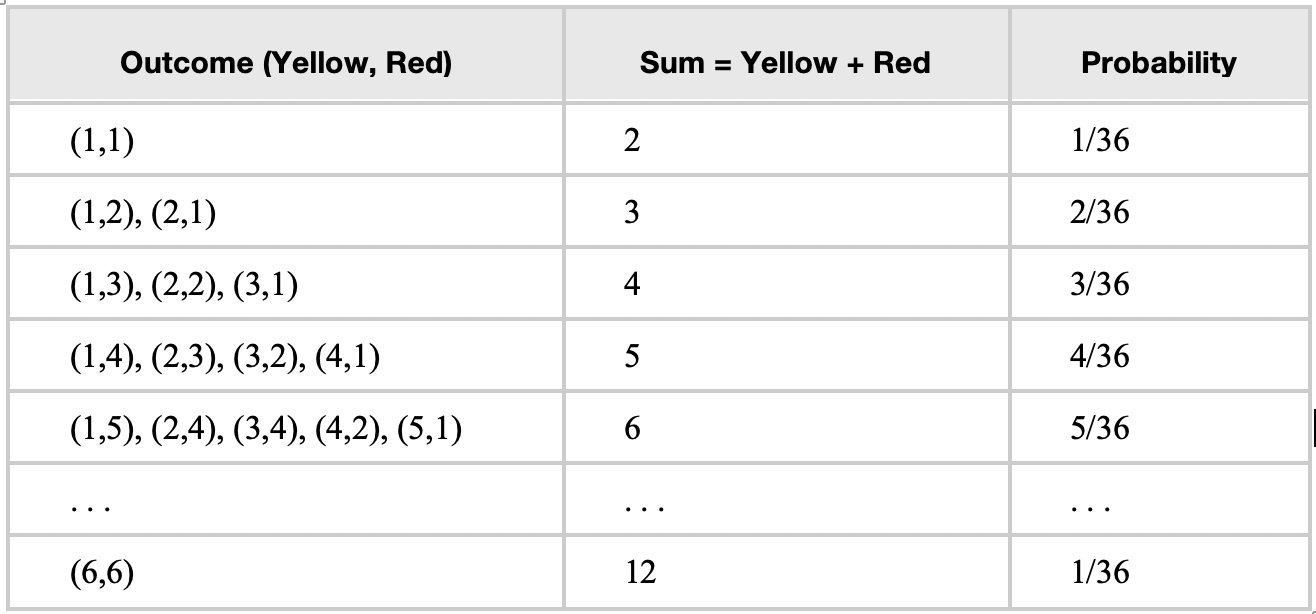
\includegraphics[width=0.5\linewidth]{topic02/TwoDiceDist} \end{center}

\begin{enumerate}
\def\labelenumi{\arabic{enumi}.}
\setcounter{enumi}{2}
\tightlist
\item
  The cumulative distribution of \(Y\) is given by
\end{enumerate}

\begin{Shaded}
\begin{Highlighting}[]
\NormalTok{knitr}\SpecialCharTok{::}\FunctionTok{include\_graphics}\NormalTok{(}\StringTok{"topic02/TwoDiceCDF.png"}\NormalTok{)}
\end{Highlighting}
\end{Shaded}

\begin{center}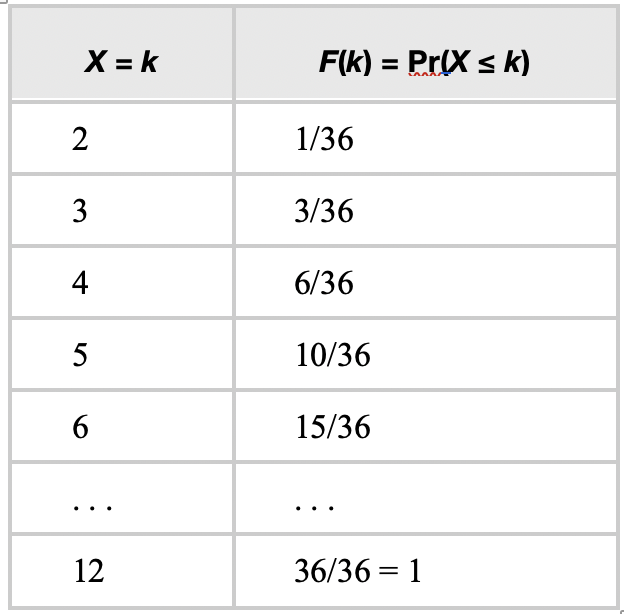
\includegraphics[width=0.28\linewidth]{topic02/TwoDiceCDF} \end{center}

\begin{enumerate}
\def\labelenumi{\arabic{enumi}.}
\setcounter{enumi}{3}
\tightlist
\item
  Using the above distribution table, we can easily find
  \[
  P(X \le 6) = 15/36 = 5/12.
  \]
\end{enumerate}

\hfill\break

\hypertarget{appendix-derivatives-of-functions}{%
\section{Appendix: Derivatives of Functions}\label{appendix-derivatives-of-functions}}

The following subsections briefly review the derivative of a single variable function.

\hypertarget{definitions-and-notations}{%
\subsection{Definitions and Notations}\label{definitions-and-notations}}

Assume \(y = f(x)\) to be a real-valued function. The \textbf{average rate of change} of \(y\) at \(x\) is given by
\[
\frac{f(x+h) - f(x)}{h}.
\]
where \(h\) is a small number close to 0.

The instantaneous rate of change at \(x\) is given by

\[
f^\prime (x) = \lim_{h\to 0} \frac{f(x+h)-f(x)}{h}
\]

The derivative of function \(f(x)\) at \(x\) is the instantaneous rate of change of \(f(x)\) at \(x\).

\hypertarget{rules-of-calculus}{%
\subsection{Rules of Calculus}\label{rules-of-calculus}}

This subsection lists the derivatives of commonly used functions.

\begin{enumerate}
\def\labelenumi{\arabic{enumi}.}
\item
  \(f(x) = c\) (c is a constant), \(f^\prime(x) = 0\).
\item
  \(f(x) = x\), \(f^\prime (x) = 1.\)
\item
  \(f(x) = ax + c\), \(f^\prime(x) = a\) (where a is a constant).
\item
  \(f(x) = x^n\), \(f^\prime(x) = nx^{n-1}\). {[}Power rule{]}
\item
  \(f(x) = e^x\), \(f^\prime (x) = e^x\).
\end{enumerate}

\(5^\prime\). \(f(x) = a^x\), \(f^\prime (x) = a^x \ln(a)\), for \(a > 0\) and \(a \ne 1\).

\begin{enumerate}
\def\labelenumi{\arabic{enumi}.}
\setcounter{enumi}{5}
\tightlist
\item
  \(f(x) = \ln (x)\), \(f^\prime (x) = 1/x\) for \(x > 0\).
\end{enumerate}

\(6^\prime\). \(f(x) = \log_a(x)\), \(f^\prime(x) = 1/[x\ln(a)]\) for \(a > 0\) and \(a \ne 1\).

\hfill\break

\textbf{Example 11}. Find \(f^\prime(x)\).

(1). \(f(x) = \frac{1}{x^2}\).

(2). \(f(x) = \log_5(x)\).

(3). \(f(x) = 2^x\).

\textbf{Solution}:

(1). Since \(f(x) = \frac{1}{x^2} = x^{-2}\), \(f^\prime (x) = (-2)x^{-2-1} = -2x^{-3}.\)

(2). \(f^\prime (x) = 1/[x\ln(5)]\).

(3). \(f^\prime (x) = 2^x \ln(2)\).

\hfill\break

\hypertarget{properties-of-derivative}{%
\subsection{Properties of Derivative}\label{properties-of-derivative}}

Let \(f(x)\) and \(g(x)\) be two real-valued functions. We have the following additive, multiplicative, quotient, and chain rules.

\begin{enumerate}
\def\labelenumi{\arabic{enumi}.}
\item
  \([f(x) \pm g(x)]^\prime = f^\prime(x) \pm g^\prime(x)\)
\item
  \([f(x)\times g(x)]^\prime = f^\prime (x)g(x) + f(x)g^\prime (x)\)
\item
  \([f(x)/g(x)]^\prime = \frac{f^\prime (x)g(x) - f(x)g^\prime (x)}{g^2(x)}\)
\item
  \([(f\circ g) (x)]^\prime = [f(g(x))]^\prime = f^\prime(g(x))g^\prime(x)\)
\end{enumerate}

\hfill\break

\textbf{Example 12}. Let \(f(x) = xe^{-(x-5)^2}\). Find \(f^\prime (x)\).

\textbf{Solution}: We use the above rules and properties to find the derivative of \(f(x)\).

\(f^\prime(x) = (x)^\prime e^{-(x -5)^2} + x[e^{-(x-5)^2}]^\prime\) {[}multiplicative rule{]}

\(\hspace{9mm}= e^{-(x -5)^2} +x e^{-(x -5)^2}[-(x-5)^2]^\prime\) {[}chain rule in the last step{]}

\(\hspace{9mm}= e^{-(x -5)^2} +x e^{-(x -5)^2}[-2(x-5)]\)

\(\hspace{9mm}= e^{-(x -5)^2}[1 -2x(x-5)]\)

\(\hspace{9mm}= e^{-(x -5)^2}[1 +10x -2x^2]\).

\hfill\break

\hypertarget{practice-exercises-1}{%
\subsection{Practice Exercises}\label{practice-exercises-1}}

\hfill\break

Worksheets \#7 - \#11 are related to the above review topics of derivatives in the following calculus worksheets bundle.

\url{https://pengdsci.github.io/WCUSTA504/Worksheet\%20Bundle.pdf}

\hfill\break

worksheet 7. Definition of the derivative\ldots\ldots\ldots\ldots\ldots\ldots\ldots\ldots\ldots\ldots\ldots\ldots\ldots\ldots\ldots\ldots. 16

worksheet 8. Computing derivatives\ldots\ldots\ldots\ldots\ldots\ldots\ldots\ldots\ldots\ldots\ldots\ldots\ldots\ldots\ldots\ldots\ldots\ldots.. 19

worksheet 9. Product and quotient rules \ldots\ldots\ldots\ldots\ldots\ldots\ldots\ldots\ldots\ldots\ldots\ldots\ldots\ldots\ldots\ldots.. 21

worksheet 10. The chain rule, and derivatives as the rate of change \ldots\ldots\ldots\ldots. 24

worksheet 11. Derivatives of logarithmic, and exponential functions \ldots\ldots\ldots.. 27

Please ignore all problems related to trigonometric functions in the above worksheets.

\hfill\break

\hypertarget{continuous-random-variables-and-their-distributions}{%
\chapter{Continuous Random Variables and Their Distributions}\label{continuous-random-variables-and-their-distributions}}

\emph{(The relevant contents can be found in Sections 4.1 -- 4.3)}

\hfill\break

This focuses on the continuous random variables and their distributions. We first gives the definition of continuous random variables and the methods for characterizing the distribution. As the simplest random variable, the uniform distribution will be discussed in this note to illustrate the steps for charactrizing the distribution of continuous random variables.

\hypertarget{continuous-random-variable-and-characterization}{%
\section{Continuous Random Variable and Characterization}\label{continuous-random-variable-and-characterization}}

\textbf{Continuous random variables} take on an uncountably infinite number of values.

\textbf{Example 1}. The following are examples of the continuous random variable.

\begin{enumerate}
\def\labelenumi{\arabic{enumi}.}
\item
  The amount of electricity generated by a nuclear plant in a day
\item
  The lifetime of an electronic component
\end{enumerate}

\hypertarget{cummulative-distribution}{%
\subsection{Cummulative Distribution}\label{cummulative-distribution}}

The \textbf{cumulative distribution function (CDF)} of a random variable Y is defined as

\[
 F(y) = P(Y \le y)
 \]
where \(- \infty < y < \infty\).

We have discussed the CDF for discrete random variables in the previous section. The following is another example.

\textbf{Example 2}: Toss a fair coin three times. Let Y denote the number of heads appearing. Noting that

\(P(Y=0) = 1/8, P(Y=1) = 3/8, P(Y =2) = 3/8, P(Y=3) = 1/8.\)

then the CDF is given by

\(F(0) = P(Y \le 0) = 1/8\).

\(F(1) = P(Y \le 1) = P(Y=0) +P(Y=1) = 1/8 + 3/8 = 1/2\).

\(F(2) = P(Y \le 2) = P(Y=0) +P(Y=1) + P(Y =2) = 1/8 + 3/8 + 3/8 = 7/8\).

\(F(3) = P(Y \le 3) = P(Y=0) +P(Y=1) + P(Y =2) = 1/8 + 3/8 + 3/8 + 1/8 = 1\).

The CDF is explicitly given by

\[
\displaystyle F_X(x) = \begin{cases} 
 1/8,  & x \le 0 ;   \\  
 4/8,  & 0 < x \le 1;  \\
 7/8,  & 1 < x \le 2 ; \\
 1,    & 2 < x \le 3;  \\
 1,    & x > 3.
 \end{cases}
\]

and the plot of the CDF is given by

\begin{center}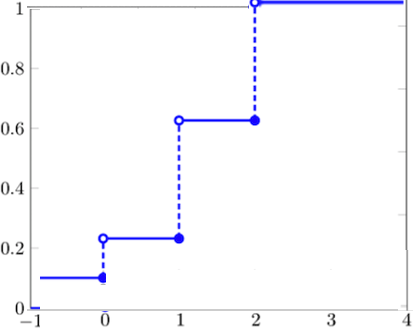
\includegraphics[width=0.3\linewidth]{topic03/CDF2CoinFigure} \end{center}

\textbf{Properties of the CDF}

\[\lim_{y \to \infty} F(y) = 1\]

\[\lim_{y \to -\infty} F(y) = 0\]

Furthermore, a CDF is a non-decreasing function of y (see the above figure) and is discontinuous for discrete random variables.

\hypertarget{cdf-of-continuous-random-variable}{%
\subsection{CDF of Continuous Random Variable}\label{cdf-of-continuous-random-variable}}

A random variable X having a continuous CDF \(F(x)\) is a continuous random variable. The probability density function (pdf) of a continuous random variable Y is defined as
,
\[
f(x) = \frac{dF(x)}{dx} = F^\prime(x)
\]
where \(-\infty < x < \infty\). Thus,

\[
F(x) = \int_{-\infty}^x f(u)du.
\]
The geometry of the above integral is depicted in the following figure.

\begin{center}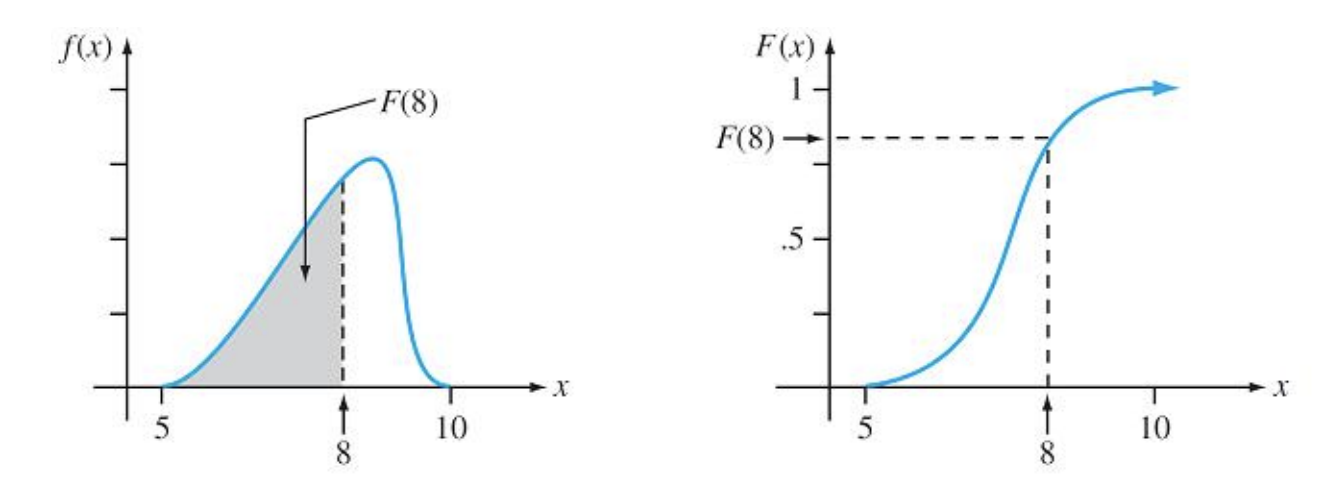
\includegraphics[width=0.6\linewidth]{topic03/CDFvsPDF} \end{center}

The area of the shaded region is the CDF of \(X\) evaluated at \(u = 8\). On the right-hand side is the curve of area vs x.

\hypertarget{properties-of-cdf-and-cdf-of-continuous-r.v.}{%
\subsection{Properties of CDF and CDF of Continuous R.V.}\label{properties-of-cdf-and-cdf-of-continuous-r.v.}}

\textbf{Properties}

Let \(f(x)\) be a real-valued function. If

\begin{enumerate}
\def\labelenumi{\arabic{enumi}.}
\item
  \(f(x) \ge 0\) and
\item
  \(\int_{-\infty}^\infty f(x) dx = 1\),
\end{enumerate}

\(f(x)\) is a probability density function (PDF) of random variable \(X\).

\textbf{Events and Probability of Continuous random variable}:

An event based on the continuous RV is defined to be an interval (including the union of a set of individual values and subintervals).

\textbf{Example 3}: Let X be a continuous random variable with probability density function (pdf) \(f(x)\). Define event \(E = (a, b)\), then

\[
P[a < X < b] = \int_a^b f(x)dx = F(b) - F(a)
\]
This event and the probability distribution are depicted in the following figure.

\begin{center}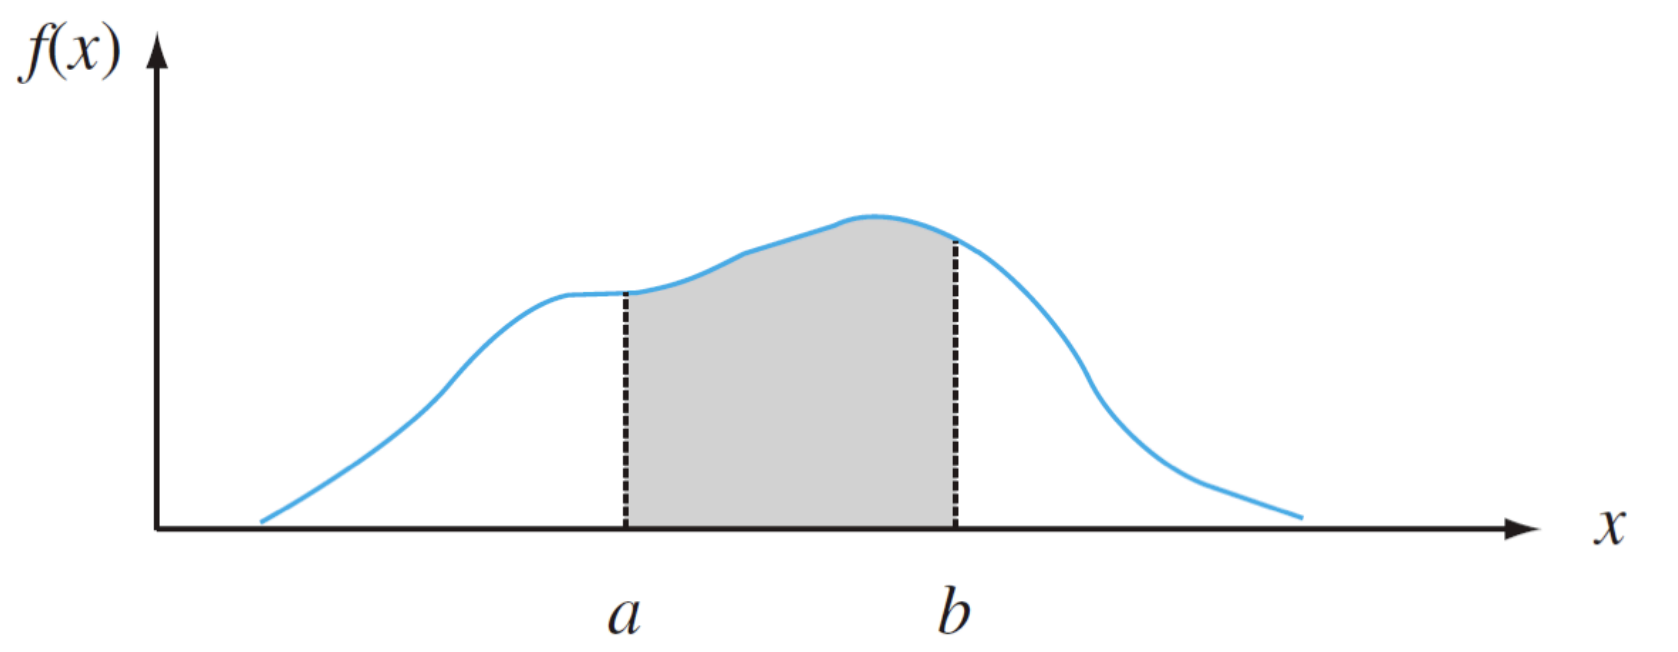
\includegraphics[width=0.6\linewidth]{topic03/ContRVevent} \end{center}

The probability that \(X\) is between a and b is the area of the shaded region.

\textbf{Example 4}: The length of time to failure (in hundreds of hours) for a transistor is a random variable Y with distribution function given by
\[
\displaystyle F(y) = \begin{cases} 
 0,  & y < 0 ;   \\  
 1-e^{-y^2},    & y \ge 0.
 \end{cases}
\]
a Show that \(F(y)\) has the properties of a distribution function.

b Find the \(.30\)-quantile, \(\phi_{0.30}\), of \(Y\).

c Find \(f(y)\).

d Find the probability that the transistor operates for at least 200 hours.

e Find \(P (Y > 100|Y \le 200)\).

\textbf{Solution}: see the \emph{board-work} in class.

\hfill\break

\hypertarget{expectation-and-variance-1}{%
\section{Expectation and Variance}\label{expectation-and-variance-1}}

Let X be a continuous random variable.

\begin{enumerate}
\def\labelenumi{\arabic{enumi}.}
\tightlist
\item
  The expectation or the expected value or the mean of X is defined as
\end{enumerate}

\[
\mu = E[X] = \int_{-\infty}^\infty yf(y)dy
\]

\begin{enumerate}
\def\labelenumi{\arabic{enumi}.}
\setcounter{enumi}{1}
\tightlist
\item
  The expected value of a function of X, denoted by \(g(x)\), is given by
\end{enumerate}

\[
E[g(X)] = \int_{-\infty}^\infty g(y)f(y)dy
\]

\begin{enumerate}
\def\labelenumi{\arabic{enumi}.}
\setcounter{enumi}{2}
\tightlist
\item
  The variance of a random variable Y is given by
\end{enumerate}

\[
 V[X] = E[(X-\mu)^2] = \int_{-\infty}^\infty (y-\mu)^2f(y)dy
 \]

The results for the expectation for discrete random variables still hold for continuous random variables (because of the linearity of the integral operator). Let c be a constant and \(g(X), g_1(X)\), and \(g_2(x)\) be functions of random variable X. Then

\begin{enumerate}
\def\labelenumi{\arabic{enumi}.}
\item
  \(E[c] = c\),
\item
  \(E[cg(X)] = c E[g(X)]\),
\item
  \(E[g_1(X) + g_2(X)] = E[g_1(X)] + E[g_2(X)]\),
\item
  \(\sigma^2 = V[X] = E[(X-\mu)^2] = E[Y^2] - \mu^2\)
\end{enumerate}

\textbf{Example 5}: Daily total solar radiation for a specified location in Florida in October has probability density
function given by

\[
\displaystyle f(y) = \begin{cases} 
 c(y-2)(6-y),  & 2 \le y \le 6;   \\  
 0,    & \text{ elsewhere}.
 \end{cases}
\]
with measurements in hundreds of calories.

\begin{enumerate}
\def\labelenumi{\alph{enumi}.}
\item
  Find the value of \(c\) to make \$f(y) a valid density function.
\item
  Find the expected daily solar radiation for October.
\item
  Find the variance of the daily solar radiation for October.
\end{enumerate}

\textbf{Solution} See the \emph{board-work} in class.

\hfill\break

We will present concrete examples when discussing special continuous random variables in the subsequent sections.

\hfill\break

\hypertarget{uniform-probability-distribution}{%
\section{Uniform Probability Distribution}\label{uniform-probability-distribution}}

\emph{(Similar contents can be found in Section 4.4)}

\hfill\break

Suppose X can take on any value within the interval \([a, b]\) , and each value in the interval is ``equally likely'' to be chosen (to be more exact, all non-overlapping sub-intervals of the same length that partition the interval \([a, b]\) are equally likely to be selected). Then \(X\) has a uniform probability distribution, and its pdf is given by

\[
\displaystyle f(x) = \begin{cases} 
 1/(b-a) & \text{if $a < x < b$} \\  
 0 & \text{otherwise}  
 \end{cases}
\]

The PDF plot is given by

\begin{center}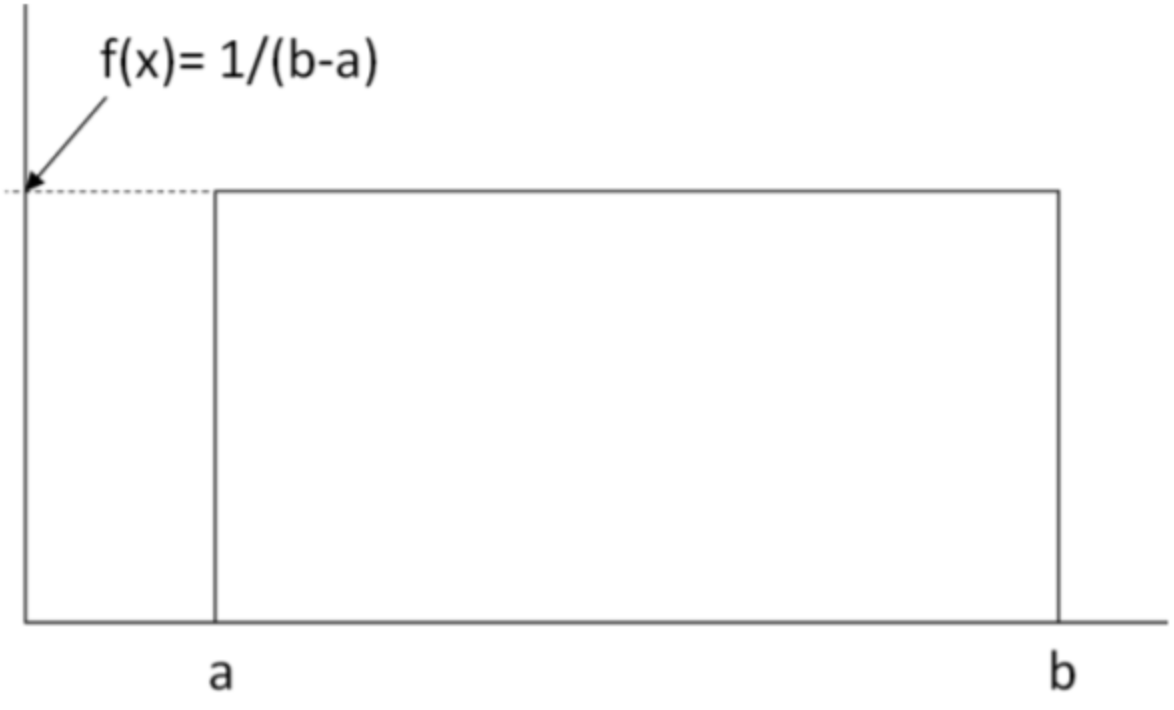
\includegraphics[width=0.4\linewidth]{topic03/uniformDensityCurve} \end{center}

The CDF and its plot are given below.

\begin{center}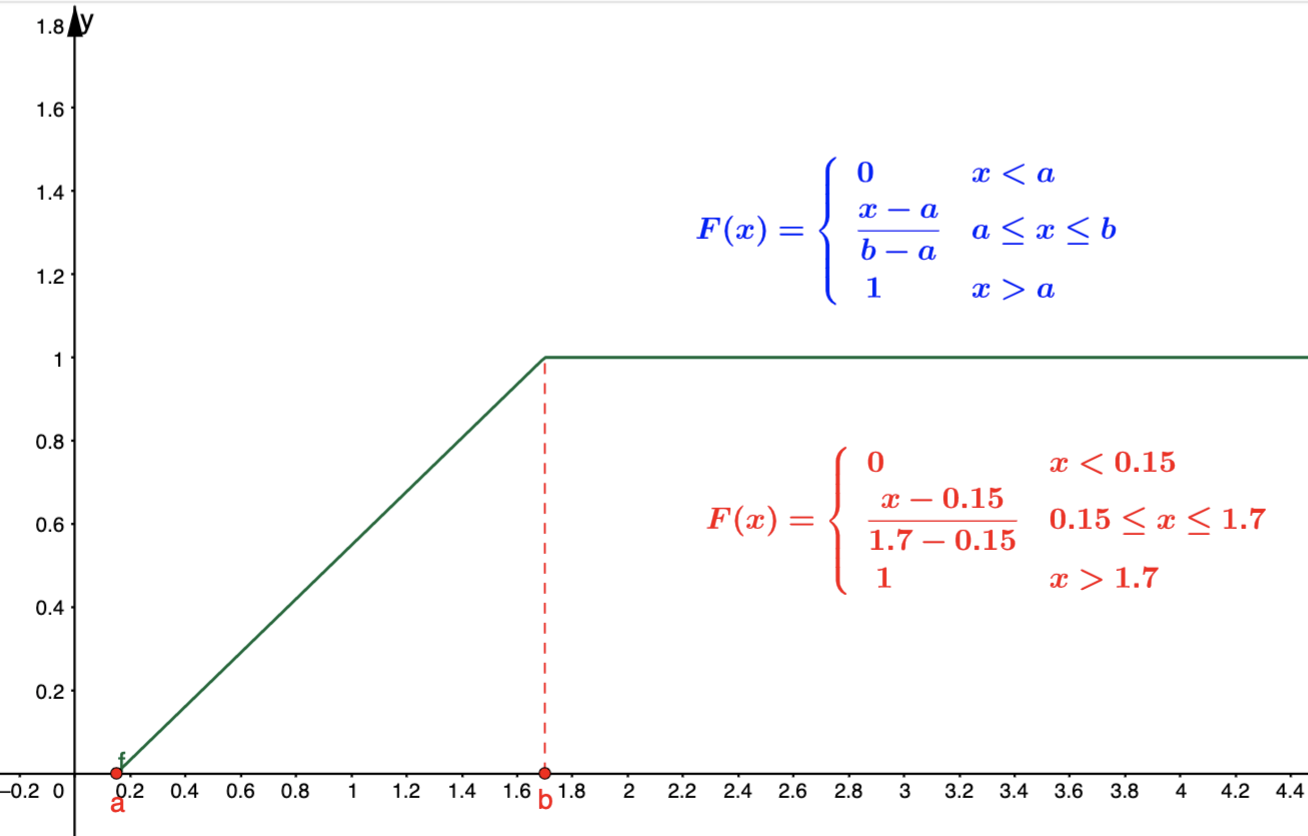
\includegraphics[width=0.6\linewidth]{topic03/unifCDF} \end{center}

\textbf{Expectation and Variance}

The mean and variance of the uniform distribution defined on the interval \([a, b]\) are given by

\[
\mu = E[X] = \int_a^b x\times \frac{1}{b-a}dx = \frac{1}{b-a}\int_a^b xdx = \frac{1}{b-a}(\frac{b^2}{2} - \frac{a^2}{2}) = \frac{a + b}{2}
\]

and

\[
\sigma^2 = V[X] = \int_a^b [x-(a+b)/2]^2 \frac{1}{b-a}dx = \cdots = \frac{(b-a)^2}{12}
\]

\textbf{A General Remark}: Finding probability and finding quantile are two practical questions for all distributions.

\hfill\break

\textbf{Example 6}: {[}\emph{Finding Probabilities}{]} Suppose the time a friend of yours will show up for a social appointment is uniformly distributed between 5 minutes before and half an hour after the appointed time.

\begin{enumerate}
\def\labelenumi{\arabic{enumi}.}
\item
  What is the probability that he will not be late?
\item
  What is the probability that he will be at least ten minutes late?
\item
  What is the probability that he will be at least 20 minutes late, given that he still has not yet arrived five minutes after the appointed time?
\end{enumerate}

\textbf{Solution}: Let \(X\) be the \emph{difference between the scheduled time and the arrival time}, then, based on the definition, \(X\) is a uniform random variable on \([-5, 30]\). Therefore, the probability density function is given by \(f(x) = 1/[30 - (-5)] = 1/35\) for \$ -5 \textless{} x \textless{} 30\$; otherwise, \(f(x) = 0\).

\begin{enumerate}
\def\labelenumi{\arabic{enumi}.}
\item
  The event ``not late'' is \([-\infty, 0]\) (arriving at the place before or on time). Therefore,
  \(P[-\infty< X <0] = P(-5 < X < 0) = [0 -(-5)]/[30 -(-5)] = 5/35 = 1/7.\)
\item
  The event ``at least 10 minutes late'' = \(X > 10\). Therefore, \(P(X > 10) = P(10 < X < 30) = [30-10]/[30-(-5)] = 20/35 = 4/7.\)
\item
  This is a conditional probability (pay attention to the ``magic word'' - \textbf{given that})! We define two events: \(A =\) not yet arrived five minutes after the appointed time \(= X > 5\) = \([5, 30]\), B = at least 20 minutes late = \(X > 20\) = \([20, 30]\). Therefore, the joint event \(A \mbox{ and } B = [20, 30]\) (overlapped part). Note that \(P[A \mbox{ and } B] = (30 - 20)/35 = 10/35 = 2/7\), \(P(A) = (30-5)/35 = 25/35 = 5/7\). Therefore, using the definition of conditional probability
\end{enumerate}

\[
P(B|A) = (2/7)/(5/7) = 2/5.
\]

\hfill\break

\hypertarget{calculus-review-integrals-of-functions}{%
\section{Calculus Review: Integrals of Functions}\label{calculus-review-integrals-of-functions}}

Finding the integral of a function is an \textbf{opposite} process of finding a derivative of a function - \textbf{antiderivative}.

\hypertarget{antiderivatives}{%
\subsection{Antiderivatives}\label{antiderivatives}}

An antiderivative (sometimes also called \texttt{inverse\ derivative}) of a function f is a differentiable function \(F(x)\) whose derivative is equal to the original function \(f(x)\).

\textbf{Example 1}. Let \(f(x) = 2x\). From the power rule of derivative, we know that \([x^2]^\prime = 2x\). This means that \(F(x) = x^2\) is the antiderivative of \(f(x) = 2x\). Note also that, \([x^2 + 5]^\prime = 2x\), that is \(G(x) = x^2 +5\). Therefore, the antiderivative of a function not unique. In general, the difference between two antiderivatives of the same original function is a constant.

\hypertarget{rules-and-properties-of-integral}{%
\subsection{Rules and Properties of Integral}\label{rules-and-properties-of-integral}}

\hypertarget{basic-rules}{%
\subsubsection{Basic Rules}\label{basic-rules}}

The following are rules of integrals. \(C\) is a real number and called \textbf{coefficient of integral}.

\begin{enumerate}
\def\labelenumi{\arabic{enumi}.}
\item
  \(f(x) = a\), then \(F(x) = \int f(x)dx = ax + C\)
\item
  \(f(x) = x^k\) (k is a constant and \(k \ne -1\)), then \(F(x) = \int x^k dx = x^{k+1}/(k+1) + C.\)
\item
  \(f(x) = 1/x = x^{-1}\), then \(F(x) = \int (1/x) dx = \ln(x) + C\)
\item
  \(f(x) = e^x\), then \(F(x) = \int e^x dx = e^x +C\)
\end{enumerate}

4.1. \(f(x) = a^x\) (\(a > 0\) and \(a \ne 1\)), then \(F(x) = a^x \ln(a)\)

\begin{enumerate}
\def\labelenumi{\arabic{enumi}.}
\setcounter{enumi}{4}
\tightlist
\item
  \(f(x) = \ln(x)\), then \(F(x) = \int \ln(x) dx = x\ln(x) - x + C\)
\end{enumerate}

\hfill\break

\hypertarget{properties-of-integrals}{%
\subsubsection{Properties of Integrals}\label{properties-of-integrals}}

\begin{enumerate}
\def\labelenumi{\arabic{enumi}.}
\item
  Multiplying a constant: \(\int af(x)dx = a\int f(x)dx\)
\item
  Additive property: \(\int [f(x) + g(x)]dx = \int f(x)dx + \int g(x)dx\)
\item
  Difference property: \(\int [f(x) - g(x)]dx = \int f(x)dx - \int g(x)dx\)
\item
  Integral by parts: \(\int f(x)dg(x) = f(x)g(x) - \int g(x)df(x)\)
\item
  Change of variable (substitution): \(\int f[g(x)] g^\prime(x)dx = \int f[g(x)] dg(x) = \int f(u)du\), where substitution \(u = g(x)\).
\end{enumerate}

\hfill\break

\hypertarget{definite-integrals}{%
\subsubsection{Definite Integrals}\label{definite-integrals}}

This is the type integrals we used to calculate the probability of an event (i.e., the union of intervals) defined based on a continuous distribution.

A \textbf{Definite Integral} has start and end values: in other words there is an interval \([a, b]\). \(a\) and \(b\) (called limits, bounds or boundaries) are put at the bottom and top of the integral sign \(\int\),

\begin{center}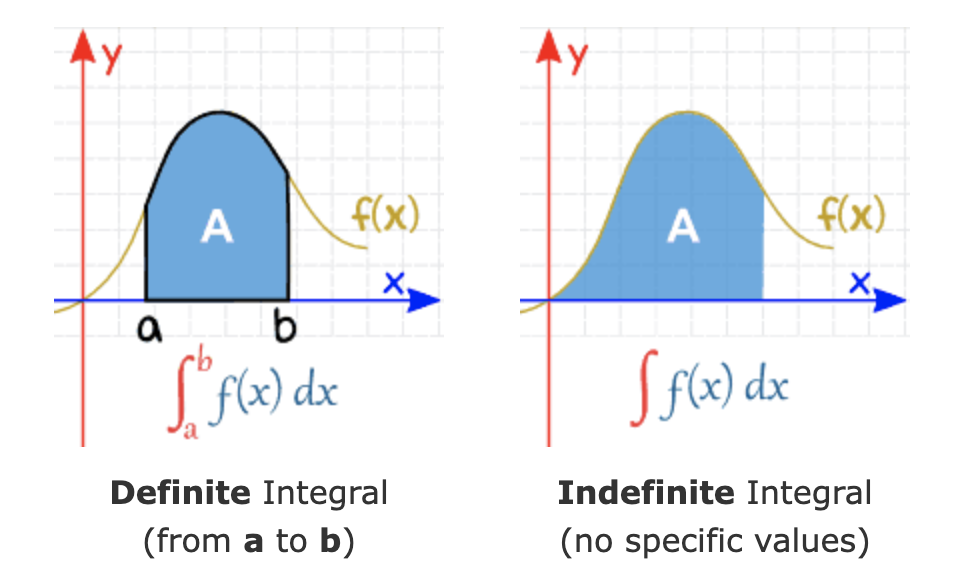
\includegraphics[width=0.5\linewidth]{topic03/Definite-Indefite} \end{center}

Let \(F(x) = \int_{-\infty}^x f(t) dt\), then definite integral \(\int_a^b f(t)dt = F(b) - F(a)\). This is called the \textbf{Fundamental Theorem of Calculus}. It is used to calculate the definite integral for a given function and the two integral limits.

\hfill\break

\textbf{Some Properties and Rules of Integrals}

\begin{enumerate}
\def\labelenumi{\arabic{enumi}.}
\item
  \(\int_a^b [f(x) \pm g(x)]dx = \int_a^b f(x)dx \pm \int_a^b g(x)dx\)
\item
  \(\int_a^b f(x)dx = -\int_b^a f(x) dx\)
\item
  \(\int_a^b f(x)dx = \int_a^c f(x)dx + \int_c^b f(x)dx\) for any constant \(c\) (\(c\) is not necessarily between \(a\) and \(b\)).
\end{enumerate}

\hfill\break

\hypertarget{practice-exercises-2}{%
\subsection{Practice Exercises}\label{practice-exercises-2}}

There two set of exercises you can practice. Ignore all problems involves trigonometric functions.

\begin{enumerate}
\def\labelenumi{\arabic{enumi}.}
\item
  Exercises with answer keys. \url{https://github.com/pengdsci/WCUSTA504/raw/main/topic03/Basic-Integration-Problems.pdf}
\item
  Worksheets: \url{https://pengdsci.github.io/WCUSTA504/Worksheet\%20Bundle.pdf}
\end{enumerate}

\begin{itemize}
\item
  Worksheet \#20: Fundamental Theorem of Calculus.
\item
  Worksheet \#21: Definite Integrals
\end{itemize}

\hfill\break

\hfill\break

\hypertarget{special-continuous-distributions-normal-and-gamma-families}{%
\chapter{Special Continuous Distributions: Normal and Gamma Families}\label{special-continuous-distributions-normal-and-gamma-families}}

We have introduced the procedures for characterizing the general continuous random variables and used the simplest well-known uniform distribution and some not-well-known distributions as examples to illustrate the properties/requirements of continuous distributions.

\hypertarget{review-of-probability-distributions}{%
\section{Review of Probability Distributions}\label{review-of-probability-distributions}}

The following is a summary.

\begin{itemize}
\tightlist
\item
  \textbf{Requirements for a probability density function (pdf)}
\end{itemize}

If function \(f(x)\) is a density function some random variable \(X\) \emph{if and only if} both of the following conditions are satisfied

\begin{enumerate}
\def\labelenumi{\arabic{enumi}.}
\item
  \(f(x) \ge 0\);
\item
  \(\int_{-\infty}^\infty f(x) dx = 1\).
\end{enumerate}

\begin{itemize}
\tightlist
\item
  \textbf{Definition of cumulative distribution function (CDF)}
\end{itemize}

Let \(f(x)\) be a pdf of random variable \(X\), and the CDF of \(X\) is defined to be

\[
P(X \le x) = F(x) = \int_{-\infty}^x f(t)dt.
\]

Note that the above CDF is defined based on the cumulative probability. Therefore, we should consider using the CDF to address problems probability associated with continuous random variables.

\hfill\break

\begin{itemize}
\tightlist
\item
  \textbf{Requirements for cumulative distribution function (CDF)}
\end{itemize}

if function \(F(x)\) is a CDF of a random variable \(X\) \emph{if and only if} all of the following conditions are satisfied.

\begin{enumerate}
\def\labelenumi{\arabic{enumi}.}
\item
  \(0 \le F(x) \le 1\);
\item
  \(F(x)\) is non-decreasing;
\item
  \(\lim_{x \to -\infty}F(x) = 0\) and \(\lim_{x \to \infty}F(x) = 1\).
\end{enumerate}

\begin{itemize}
\tightlist
\item
  \textbf{Relationship between pdf and CDF}
\end{itemize}

The relationship between pdf and CDF can be easily observed from the definition of CDF: \(F^\prime(x) = f(x)\).

\begin{itemize}
\tightlist
\item
  \textbf{Expectations and Properties}
\end{itemize}

Let \(f(x)\) be the density function of \(X\) and \(g(X)\) is a function of random variable \(X\). Apparently, \$G(X) is also a random variable.

\begin{enumerate}
\def\labelenumi{\arabic{enumi}.}
\item
  Expectation of \(X\) is defined as \(\mu = E[X] = \int_{-\infty}^\infty x f(x)dx\).
\item
  The expectation of \(g(X)\) is defined to be \(E[g(X)] = \int_{-\infty}^\infty g(x) f(x)dx\).
\end{enumerate}

As a special case of the above property 2. We can find the variance of \(X\) in the following

\begin{enumerate}
\def\labelenumi{\arabic{enumi}.}
\setcounter{enumi}{2}
\tightlist
\item
  \(V[X] = E[(X - \mu)^2] = \int_{-\infty}^\infty (X - \mu)^2f(x)dx = E[X^2] - \mu^2.\)
\end{enumerate}

\hfill\break

The next example is related to a very well-known distribution. We need to use two important rules of integral: integral by part and substitution.

\textbf{Example 1}: A random variable \(Y\) has the density function

\[
\displaystyle f(y) = \begin{cases} 
 \theta e^{-\theta y} & \text{if $y \ge 0$}, \\  
 0 & \text{otherwise}.
 \end{cases}
\]

a). Prove that \(f(y)\) is a valid density function.

b). Find the CDF of \(Y\).

c). Find \(E[Y]\) and \(V[Y]\).

d). Find \(E[e^{3Y/2}]\).

\textbf{Solution} See the \emph{board work} in the class.

a). \(\int_0^\infty f(y)dy = \int_0^\infty \theta e^{-\theta y} dy = - \int_0^\infty e^{-\theta y} d(\theta y) = -\theta e^{-\theta y}|_0^\infty = - (0 - 1) = 1\). This implies that the given function is a valid density function for \(\theta >0\).

We have used substitution in the above derivation (the first equation): if letting \(w = -\theta y\) (substitution!), then \(\int_0^\infty e^{-\theta y} d(-\theta y) = \int_0^\infty e^wdw = e^w|_0^\infty\).

b). The CDF for \(Y\) is defined to be
\[
F(y) = \int_{-\infty}^y f(x)dx = \int_0^y \theta e^{-\theta x} dx = -\int_0^y e^{-\theta y}d(-\theta y) = -e^{-\theta y}|_0^y = -(e^{-\theta y} - 1) = 1 - e^{-\theta y}.
\]

for \(y \ge 0\). \(F(x) = 0\) if \(y<0\). We have used substitution in the above derivation (the third equation) implicitly.

c). \(E[Y] = \int_0^\infty y \theta e^{-\theta y}dy =-\int_0^\infty y e^{-\theta y}d(-\theta y)\) (substitution)
\(= -y \int_0^\infty y d(e^{-\theta y}) = -[ye^{-\theta y}|_0^\infty-\int_0^\infty e^{-\theta y} dy]\) (integral by parts)
\(= -[(0 - 0) - \int_0^\infty e^{-\theta y} dy] = (1/\theta) \int_0^\infty \theta e^{-\theta y} dy = 1/\theta.\)

Note that the variance \(V[Y] = E[Y^2] - \mu^2\). To find the variance, we only need to calculate the second moment.
\[
E[Y^2] = \int_0^\infty y^2 \theta e^{-\theta y}dy = -\int_0^\infty y^2 e^{-\theta y}d(-\theta y)dy = -\int_0^\infty y^2 d(e^{-\theta y})dy \\ =  -[y^2e^{-\theta y}|_0^\infty -\int_0^\infty e^{-\theta y }dy^2] = \int_0^\infty e^{-\theta y}(2y)dy = 2\int_0^\infty ye^{-\theta y}dy \\ = \frac{2}{\theta} \int_0^\infty y \theta e^{-\theta y}dy 
 = \frac{2}{\theta} \times \frac{1}{\theta} = \frac{2}{\theta^2}
 \]

Therefore,
\[
V[Y] = E[Y^2] - \mu^2 = \frac{2}{\theta^2} - (\frac{1}{\theta})^2 = \frac{1}{\theta^2}.
\]

d). \(E[e^{3Y/2}] = \int_0^\infty e^{3y/2} \theta e^{-\theta y} dy = \int_0^\infty \theta e^{3y/2-\theta y}dy = \int_0^\infty \theta e^{-(\theta - 3/2)y}dy\) \(= \frac{\theta}{\theta-3/2} \int_0^\infty (\theta-3/2)e^{-(\theta-3/2)y} dy = \frac{\theta}{\theta - 3/2}\).

\hfill\break

\hypertarget{normal-distribution}{%
\section{Normal Distribution}\label{normal-distribution}}

\emph{(Similar contents can be found in Section 4.5)}

\hfill\break

Let \(X\) be a normal random variable or is normally distributed with mean \(\mu\) and variance \(\sigma^2\) if the pdf of \(X\) is given by

\[
 f(x) = \frac{1}{\sqrt{2\pi}\sigma} e^{-\frac{(x-\mu)}{2\sigma^2}}
 \]
with \(-\infty < x < \infty\).

After some algebra, we can check the expectation and variance of X in the following.

\[
E[X] = \int_{-\infty}^\infty xf(x)dx = \mu
\]
and

\[
V[X] = \int_{-\infty}^\infty (x-\mu)^2f(x)dx = \sigma^2 
\]

The density curve of the normal distribution has the following form

\begin{center}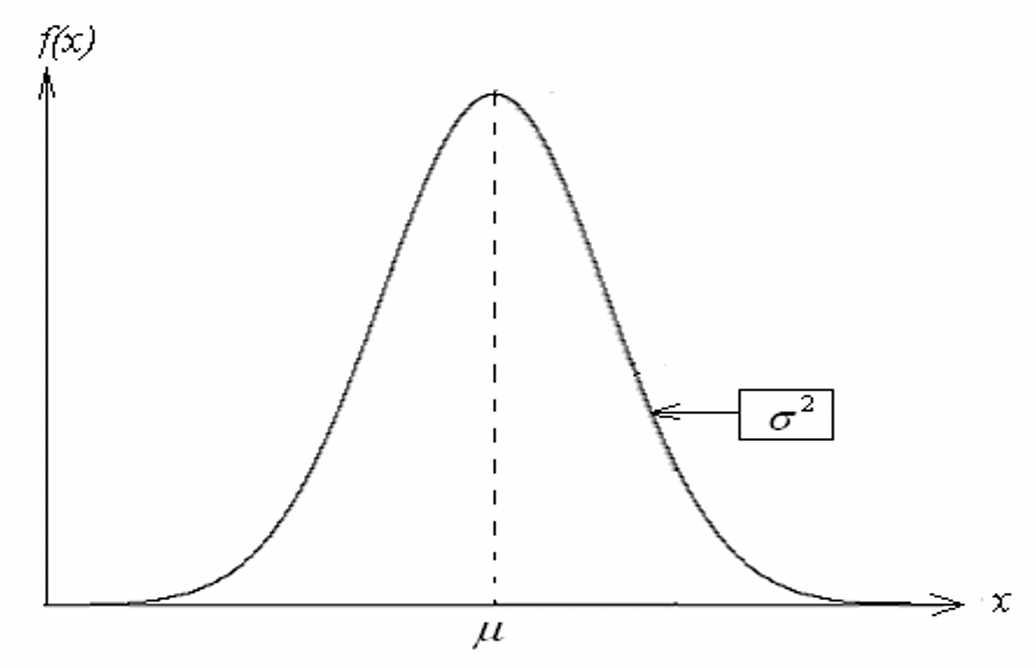
\includegraphics[width=0.4\linewidth]{topic03/normalDensity} \end{center}

\textbf{Special Case - Standard Normal Distribution}:

When \(\mu = 0\) and \(\sigma = 1\), the general normal distribution reduces to the standard normal distribution.

\hfill\break

The two basic types of questions: finding probability and finding quantile

\hfill\break

\begin{center}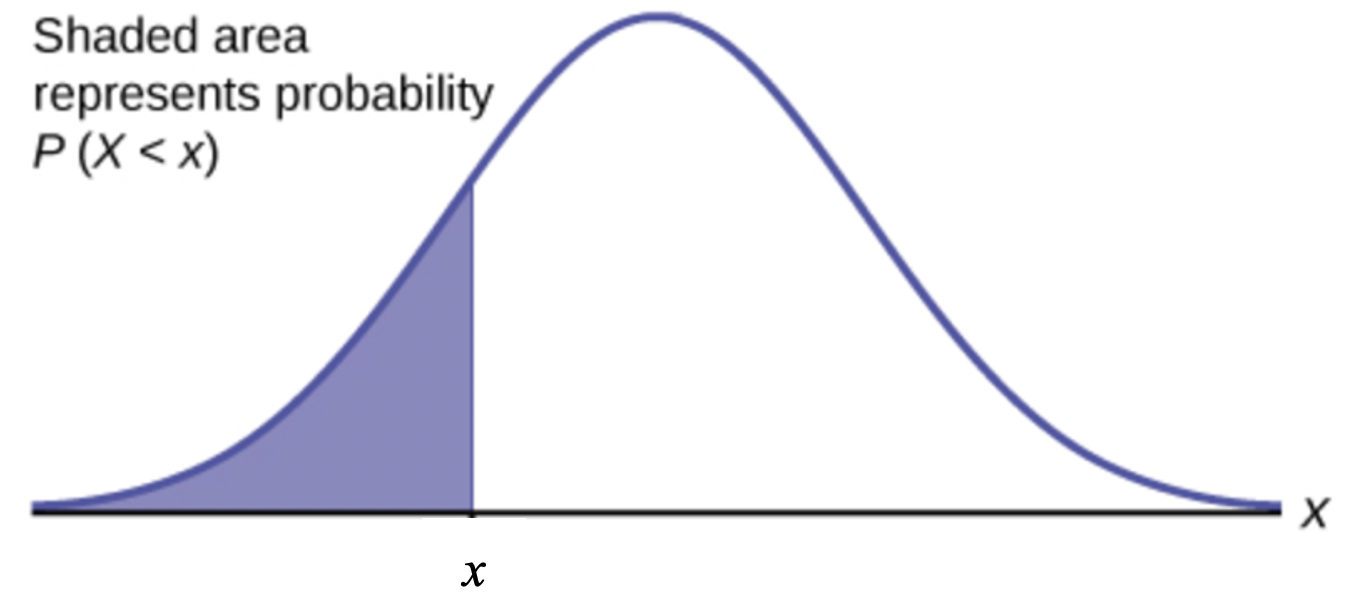
\includegraphics[width=0.4\linewidth]{topic03/normalTailArea} \end{center}

\textbf{Finding Probabilities}

Finding \(P(X < x)\) (i.e., the left-tail area) for given \(x\).

\textbf{Finding Percentiles}

Finding \(x\) from \(P(X<x) = p\) for given \(p\) (the left-tail area).

There are no formulas for finding probability and quantile based on the normal distribution. We can use either \textbf{software programs} or the \textbf{standard normal table} to answer the above two types of questions.

In R, there are functions to find probabilities and quantiles.

\begin{verbatim}
dnorm(x, mean = 0, sd = 1, log = FALSE)
# left-tail probability
pnorm(q, mean = 0, sd = 1, lower.tail = TRUE, log.p = FALSE)   
# quantile for given left-tail probability
qnorm(p, mean = 0, sd = 1, lower.tail = TRUE, log.p = FALSE)   
rnorm(n, mean = 0, sd = 1)
\end{verbatim}

\textbf{Example 2}. The final exam scores in a statistics class were normally distributed with a mean of 63 and a standard deviation of five.

\begin{enumerate}
\def\labelenumi{\arabic{enumi}.}
\item
  Find the probability that a randomly selected student scored more than 65 on the exam.
\item
  Find the probability that a randomly selected student scored less than 85.
\item
  Find the 90th percentile (that is, find the score \(k\) that has 90\% of the scores below \(k\) and 10\% of the scores above \(k\)).
\item
  Find the 70th percentile (that is, find the score \(k\) such that 70\% of scores are below \(k\) and 30\% of the scores are above \(k\)).
\end{enumerate}

\textbf{Solution}: We will use R functions to answer the above questions.

\begin{enumerate}
\def\labelenumi{\arabic{enumi}.}
\tightlist
\item
  We want to find the right-tail area. R function \texttt{pnorm} can be used to find either left-tail or right-tail area. By default, it yields the left-tail area.
\end{enumerate}

\begin{center}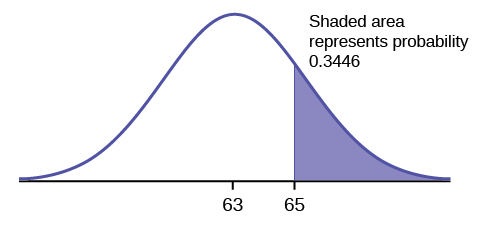
\includegraphics[width=0.4\linewidth]{topic03/exmple5-1} \end{center}

\begin{Shaded}
\begin{Highlighting}[]
\FunctionTok{pnorm}\NormalTok{(}\AttributeTok{q =} \DecValTok{65}\NormalTok{, }\AttributeTok{mean =} \DecValTok{63}\NormalTok{, }\AttributeTok{sd =} \DecValTok{5}\NormalTok{, }\AttributeTok{lower.tail =} \ConstantTok{FALSE}\NormalTok{)}
\end{Highlighting}
\end{Shaded}

\begin{verbatim}
## [1] 0.3445783
\end{verbatim}

\begin{enumerate}
\def\labelenumi{\arabic{enumi}.}
\setcounter{enumi}{1}
\tightlist
\item
  This probability is equal to the left-tail area and can be found in the following R function
\end{enumerate}

\begin{Shaded}
\begin{Highlighting}[]
\FunctionTok{pnorm}\NormalTok{(}\AttributeTok{q =} \DecValTok{85}\NormalTok{, }\AttributeTok{mean =} \DecValTok{63}\NormalTok{, }\AttributeTok{sd =} \DecValTok{5}\NormalTok{)}
\end{Highlighting}
\end{Shaded}

\begin{verbatim}
## [1] 0.9999946
\end{verbatim}

\begin{enumerate}
\def\labelenumi{\arabic{enumi}.}
\setcounter{enumi}{2}
\tightlist
\item
  We need to use R quantile function \texttt{qnorm()} to find the quantile.
\end{enumerate}

\begin{center}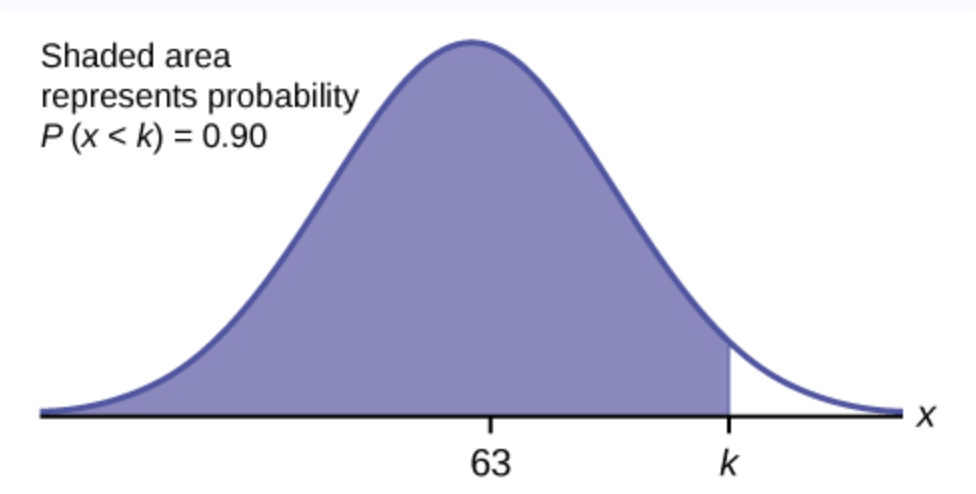
\includegraphics[width=0.4\linewidth]{topic03/exmple5-2} \end{center}

\begin{Shaded}
\begin{Highlighting}[]
\FunctionTok{qnorm}\NormalTok{(}\AttributeTok{p =} \FloatTok{0.9}\NormalTok{, }\AttributeTok{mean =} \DecValTok{63}\NormalTok{, }\AttributeTok{sd =} \DecValTok{5}\NormalTok{)}
\end{Highlighting}
\end{Shaded}

\begin{verbatim}
## [1] 69.40776
\end{verbatim}

\begin{enumerate}
\def\labelenumi{\arabic{enumi}.}
\setcounter{enumi}{3}
\tightlist
\item
  70th percentile can be found using the following R command.
\end{enumerate}

\begin{Shaded}
\begin{Highlighting}[]
\FunctionTok{qnorm}\NormalTok{(}\AttributeTok{p =} \FloatTok{0.7}\NormalTok{, }\AttributeTok{mean =} \DecValTok{63}\NormalTok{, }\AttributeTok{sd =} \DecValTok{5}\NormalTok{)}
\end{Highlighting}
\end{Shaded}

\begin{verbatim}
## [1] 65.622
\end{verbatim}

\hfill\break

\textbf{Example 3}. A personal computer is used for office work at home, research, communication, personal finances, education, entertainment, social networking, and a myriad of other things. Suppose that the average number of hours a household personal computer is used for entertainment is two hours per day. Assume the times for entertainment are normally distributed and the standard deviation for the times is half an hour.

\begin{enumerate}
\def\labelenumi{\arabic{enumi}.}
\item
  Find the probability that a household personal computer is used for entertainment between 1.8 and 2.75 hours per day.
\item
  Find the maximum number of hours per day that the bottom quartile of households uses a personal computer for entertainment.
\end{enumerate}

\textbf{Solution}. We still use R functions to answer these two questions.

\begin{enumerate}
\def\labelenumi{\arabic{enumi}.}
\tightlist
\item
  We find probability \(P(1.8 < X < 2.75)\).
\end{enumerate}

\begin{Shaded}
\begin{Highlighting}[]
\FunctionTok{pnorm}\NormalTok{(}\AttributeTok{q =} \FloatTok{2.75}\NormalTok{, }\AttributeTok{mean =} \DecValTok{2}\NormalTok{, }\AttributeTok{sd =} \FloatTok{0.5}\NormalTok{) }\SpecialCharTok{{-}} \FunctionTok{pnorm}\NormalTok{(}\AttributeTok{q =} \FloatTok{1.8}\NormalTok{, }\AttributeTok{mean =} \DecValTok{2}\NormalTok{, }\AttributeTok{sd =} \FloatTok{0.5}\NormalTok{)}
\end{Highlighting}
\end{Shaded}

\begin{verbatim}
## [1] 0.5886145
\end{verbatim}

\begin{center}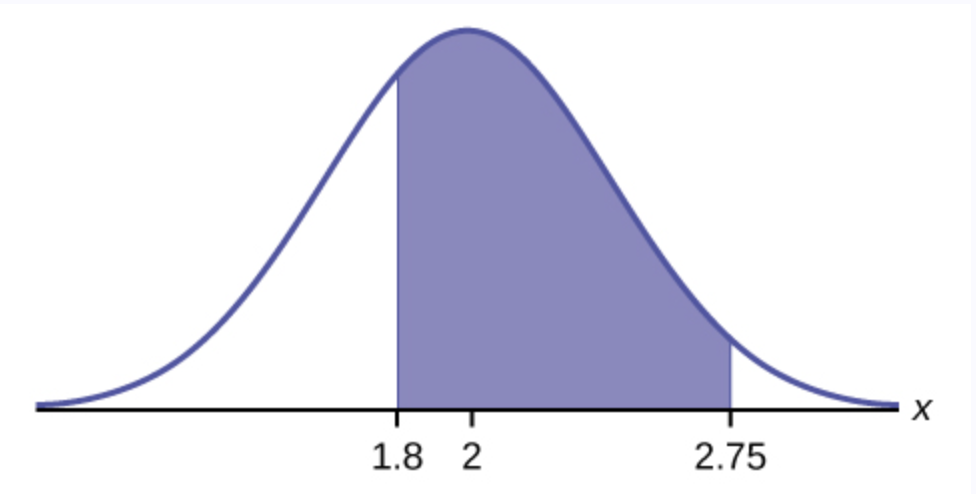
\includegraphics[width=0.4\linewidth]{topic03/example6-1} \end{center}

The probability that a household personal computer is used between 1.8 and 2.75 hours per day for entertainment is 0.5886.

\begin{enumerate}
\def\labelenumi{\arabic{enumi}.}
\setcounter{enumi}{1}
\tightlist
\item
  This is percentile question. R function \texttt{qnorm()} will be used.
\end{enumerate}

\begin{Shaded}
\begin{Highlighting}[]
\FunctionTok{qnorm}\NormalTok{(}\AttributeTok{p =} \FloatTok{0.25}\NormalTok{, }\AttributeTok{mean =} \DecValTok{2}\NormalTok{, }\AttributeTok{sd =} \FloatTok{0.5}\NormalTok{)}
\end{Highlighting}
\end{Shaded}

\begin{verbatim}
## [1] 1.662755
\end{verbatim}

\begin{center}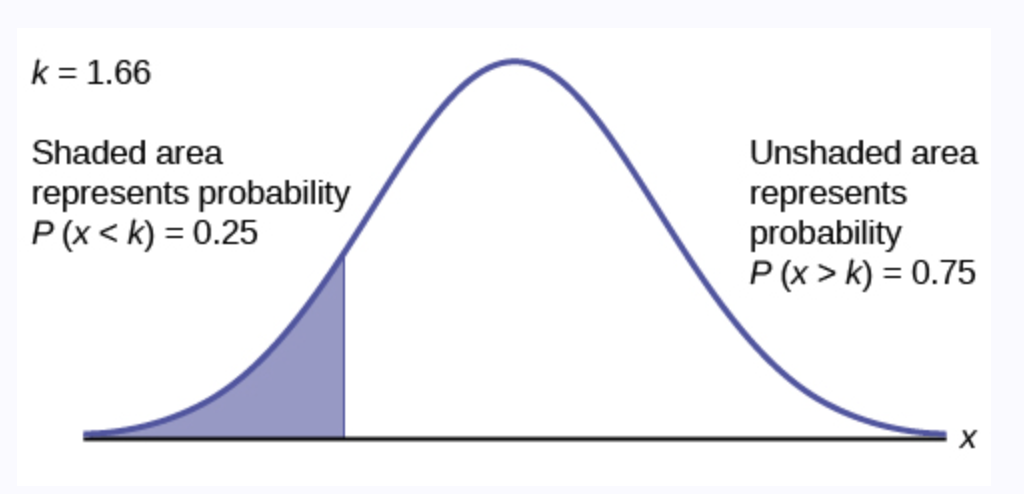
\includegraphics[width=0.4\linewidth]{topic03/example6-2} \end{center}

The maximum number of hours per day that the bottom quartile of households uses a personal computer for entertainment is 1.66 hours.

\hfill\break

\hypertarget{gamma-distribution}{%
\section{Gamma Distribution}\label{gamma-distribution}}

\emph{(Similar contents can be found in Section 4.6)}

\hfill\break

The gamma distribution contains two special and practically important members: exponential and \(\chi^2\) distributions. The PDF of gamma involves a special gamma function.

\hypertarget{the-gamma-function}{%
\subsection{The Gamma Function}\label{the-gamma-function}}

The gamma function is defined by

\[
\Gamma(r) = \int_0^\infty r^{r-1}e^{-t}dt, r > 0.
\]

It has the property that

\[
\Gamma(r+1) = r\Gamma(r), r > 1.
\]
For a positive integer \(n\), \(\Gamma(n+1) = n\Gamma(n) = \cdots = n!\).

.

\hypertarget{definition-of-gamma-density}{%
\subsection{Definition of Gamma Density}\label{definition-of-gamma-density}}

Gamma distribution has two different forms (reparameterization). Our textbook uses the following form

\[
\displaystyle f(x) = \begin{cases} 
 \frac{x^{\alpha-1}e^{-x/\beta}}{\beta^\alpha\Gamma(\alpha)} & \text{if $0 < x < \infty$} \\  
 0 & \text{otherwise}  
 \end{cases}
\]

Density curves with various values of parameters \(\alpha\) (shape) and \(\beta\) (scale).

The CDF is defined as

\[
F(x) = \int_0^y \frac{y^{\alpha-1}e^{-y/\beta}}{\beta^\alpha\Gamma(\alpha)} dy
\]

The following figures show the density curves and their corresponding CDF curves based on different values of gamma parameters.

\begin{center}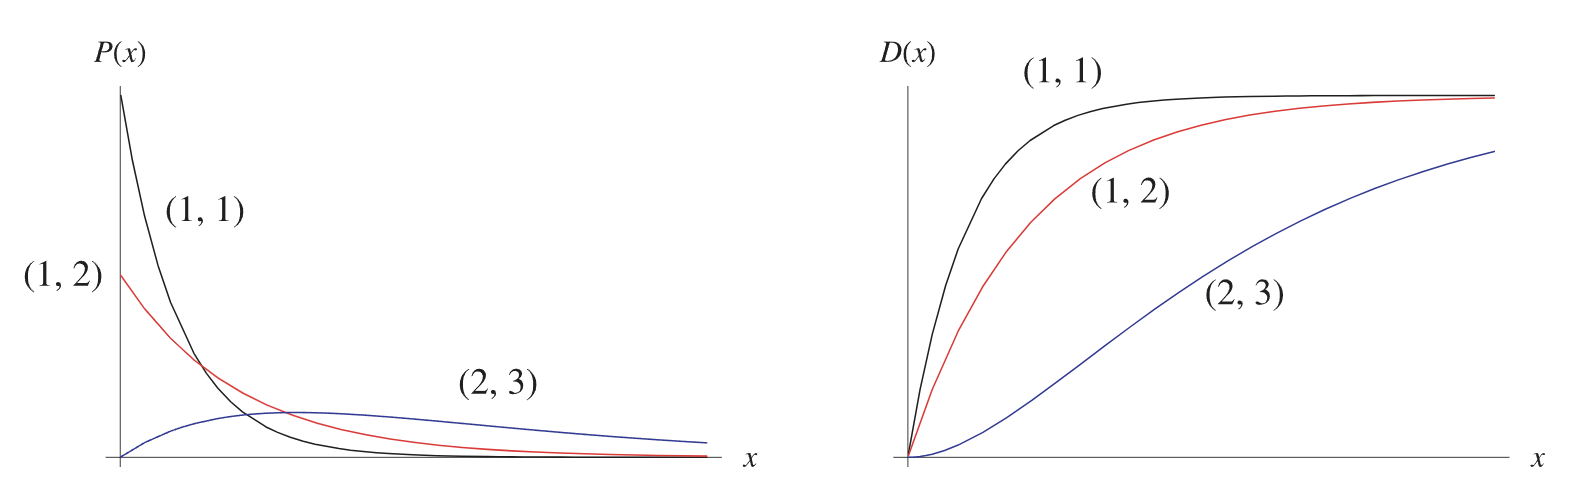
\includegraphics[width=0.7\linewidth]{topic03/gammaCDF-PDF} \end{center}

\hfill\break

\hypertarget{expectation-and-variance-2}{%
\subsection{Expectation and Variance}\label{expectation-and-variance-2}}

Using the definition of expectation and variance, we can derive the formulas of the expectation and variance of gamma distribution in the following:

\[
E[X] = \int_0^\infty x \frac{x^{\alpha-1}e^{-x/\beta}}{\beta^\alpha\Gamma(\alpha)} dx = \alpha\beta
\]
and

\[
V[X] = \int_0^\infty (x-\alpha\beta)^2 \frac{x^{\alpha-1}e^{-x/\beta}}{\beta^\alpha\Gamma(\alpha)} dx = \alpha\beta^2
\]

The detailed derivation of the above two formulas can be found on page 187 of the textbook.

\hfill\break

\hypertarget{special-cases-1}{%
\subsection{Special Cases}\label{special-cases-1}}

\begin{itemize}
\tightlist
\item
  If \(\alpha = 1\), the gamma distribution is reduced to the well-known exponential distribution with the following density function.
\end{itemize}

\[
\displaystyle f(x) = \begin{cases} 
 \frac{e^{-x/\beta}}{\beta} & \text{if $0 < x < \infty$} \\  
 0 & \text{otherwise}  
 \end{cases}
\]

The expectation and variance of the exponential distribution are \(E[X] = \beta\) and \(V[X] = \beta^2\).

The exponential distribution has been widely used in reliability and survival analysis as a base model since it is mathematically simple.

\begin{itemize}
\tightlist
\item
  If \(a = \nu/2\) and \(\beta = 2\), the gamma distribution is reduced to the well-known \(\chi^2\) distribution with \(\nu\) degrees of freedom. We define the \(\chi^2\) from the normal distribution in subsequent notes.
\end{itemize}

The expectation and variance of \(\chi_\nu^2\) is simple: \(E[X] = \nu\) and \(V[X] = 2\nu\).

\hfill\break

\hypertarget{use-of-technology}{%
\subsection{Use of Technology}\label{use-of-technology}}

The exponential and \(\chi^2\) distributions are special members of the gamma family. R has standalone sets of functions for these distributions.

Special attention should be paid to the form (reparameterization) of the gamma and exponential distributions. R uses the same form as what we used in this note. We will use several examples to show how to use these R functions.

\hypertarget{related-r-functions-for-gamma-distributions}{%
\subsubsection{Related R Functions for Gamma Distributions}\label{related-r-functions-for-gamma-distributions}}

\emph{(Help document: \url{https://stat.ethz.ch/R-manual/R-devel/library/stats/html/GammaDist.html})}

\begin{verbatim}
dgamma(x, shape, rate = 1, scale = 1/rate, log = FALSE)
pgamma(q, shape, rate = 1, scale = 1/rate, lower.tail = TRUE, log.p = FALSE)
qgamma(p, shape, rate = 1, scale = 1/rate, lower.tail = TRUE, log.p = FALSE)
rgamma(n, shape, rate = 1, scale = 1/rate)
\end{verbatim}

\textbf{Example 4}. Engineers designing the next generation of space shuttles plan to include two fuel pumps ---one active, the other in reserve. If the primary pump malfunctions, the second is automatically brought online. Suppose that the time to failure of the first pump, denoted by \(X\), is a gamma distribution with a mean of 200 and a variance of 20000. What are the chances that such a fuel pump system would not remain functioning for the full 50 hours?

\textbf{Solution}. Since \(E[X] = \alpha\beta = 200\) and \(V[X] = \alpha \beta^2 = 20000\), we solve the shape (\(\alpha\)) and scale (\(\beta\)) and obtain \(\alpha = 2\) and \(\beta = 100\). Therefore, the density function of this gamma distribution is given by

\[
f(x) = \frac{1}{100^2\Gamma(2)}e^{-x/100} x^{2-1} = \frac{1}{10000}ye^{-x/100}, \mbox{ for } x \ge 0.
\]
The probability \(P(X < 50)\) can be found using R function \texttt{pgamma()}.

\begin{Shaded}
\begin{Highlighting}[]
\FunctionTok{pgamma}\NormalTok{(}\AttributeTok{q=}\DecValTok{50}\NormalTok{, }\AttributeTok{shape =} \DecValTok{2}\NormalTok{, }\AttributeTok{scale =} \DecValTok{100}\NormalTok{)}
\end{Highlighting}
\end{Shaded}

\begin{verbatim}
## [1] 0.09020401
\end{verbatim}

The area of the shaded region in the following density curve is the probability.

\begin{center}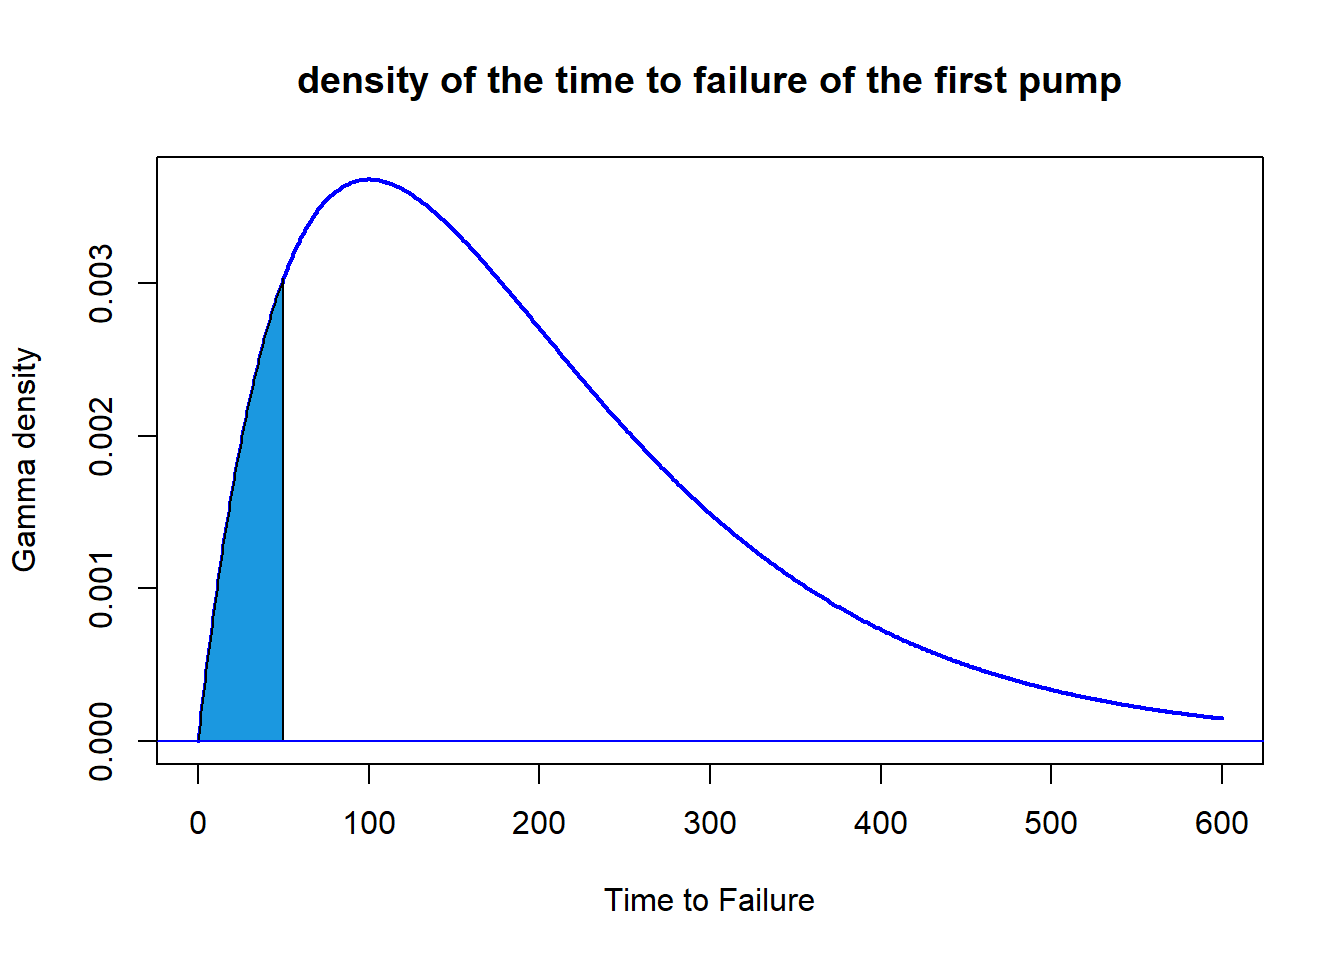
\includegraphics{STA504EB_files/figure-latex/unnamed-chunk-61-1} \end{center}

\hfill\break

\hypertarget{related-r-functions-for-exponential-distributions}{%
\subsubsection{Related R Functions for Exponential Distributions}\label{related-r-functions-for-exponential-distributions}}

\emph{(Help Document: \url{https://stat.ethz.ch/R-manual/R-devel/library/stats/html/Exponential.html})}

\begin{verbatim}
dexp(x, rate = 1, log = FALSE)
pexp(q, rate = 1, lower.tail = TRUE, log.p = FALSE)
qexp(p, rate = 1, lower.tail = TRUE, log.p = FALSE)
rexp(n, rate = 1)
\end{verbatim}

\textbf{Example 5}. The number of miles that a particular car can run before its battery wears out is exponentially distributed with an average of 10,000 miles. The owner of the car needs to take a 5000-mile trip. What is the probability that he will be able to complete the trip without having to replace the car battery?

\textbf{Solution}: In R, the exponential related R function uses the following form
\[
f(x) = \lambda e^{-\lambda x}, \mbox{ for } x \ge 0.
\]

Based on the above density form, we have \(E[X] = 1/\lambda\). Since \(1/\lambda = 10000\), \(\lambda = 1/10000\). Therefore, the desired probability \(P(X > 5000)\) (upper tail) can be found using the following R function.

\begin{Shaded}
\begin{Highlighting}[]
\FunctionTok{pexp}\NormalTok{(}\DecValTok{5000}\NormalTok{, }\AttributeTok{rate =} \DecValTok{1}\SpecialCharTok{/}\DecValTok{10000}\NormalTok{,  }\AttributeTok{lower.tail =} \ConstantTok{FALSE}\NormalTok{)}
\end{Highlighting}
\end{Shaded}

\begin{verbatim}
## [1] 0.6065307
\end{verbatim}

\begin{center}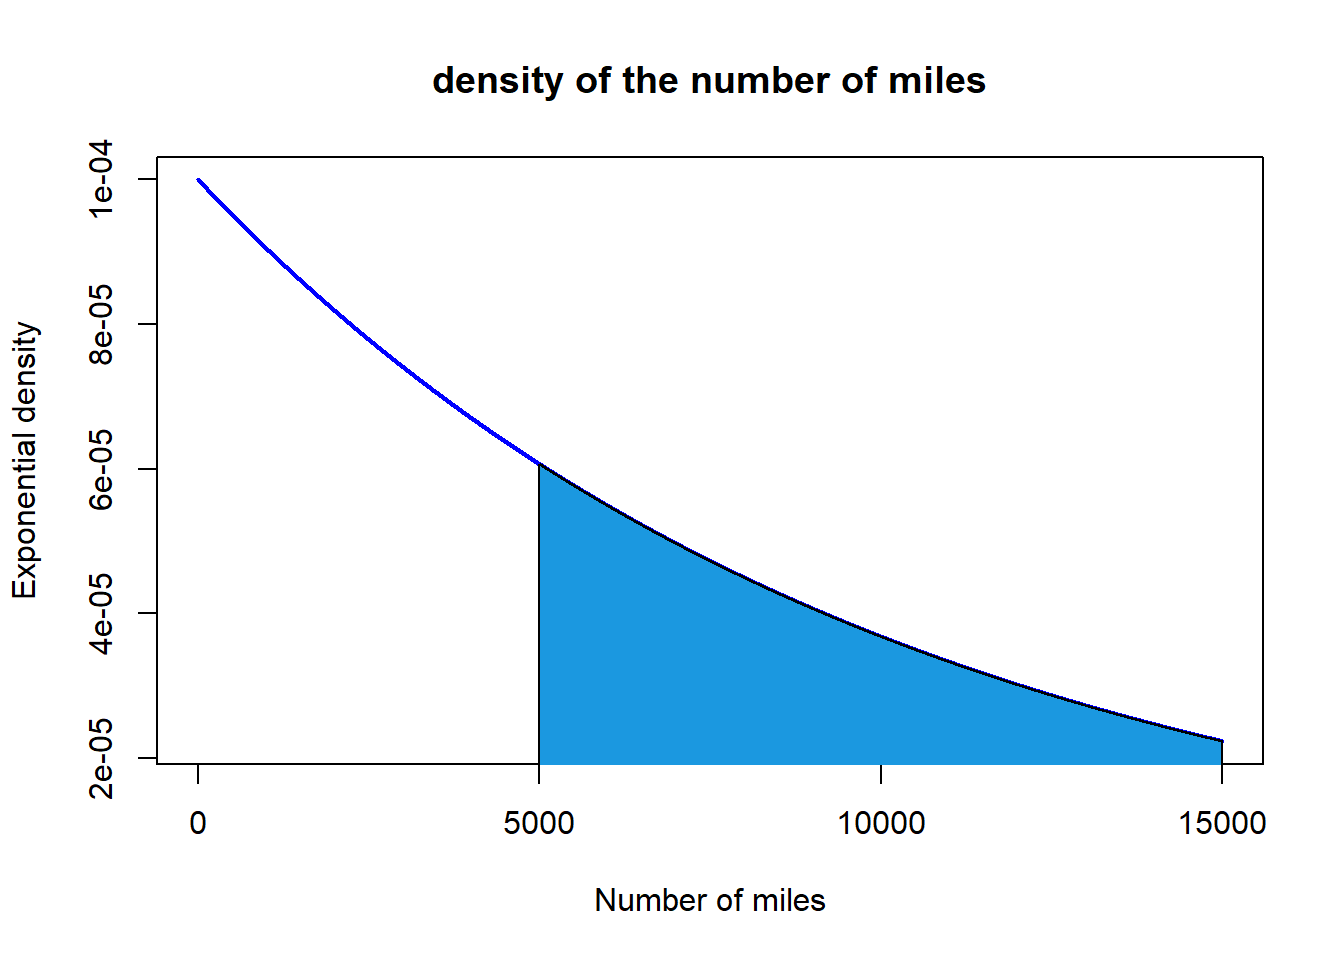
\includegraphics{STA504EB_files/figure-latex/unnamed-chunk-63-1} \end{center}

\hfill\break

\hypertarget{related-r-functions-for-chi_df2-distributions}{%
\subsubsection{\texorpdfstring{Related R Functions for \(\chi_{df}^2\) Distributions}{Related R Functions for \textbackslash chi\_\{df\}\^{}2 Distributions}}\label{related-r-functions-for-chi_df2-distributions}}

\emph{(Help Document: \url{https://stat.ethz.ch/R-manual/R-devel/library/stats/html/Chisquare.html})}

\begin{verbatim}
dchisq(x, df, ncp = 0, log = FALSE)
pchisq(q, df, ncp = 0, lower.tail = TRUE, log.p = FALSE)
qchisq(p, df, ncp = 0, lower.tail = TRUE, log.p = FALSE)
rchisq(n, df, ncp = 0)
\end{verbatim}

The \(\chi^2\) distribution is one of the most commonly used distributions and will be used to define the \(\chi^2\) test. We will not present examples in this note. But it will be used later.

\hfill\break

\hypertarget{calculus-review-integrals-of-functions-1}{%
\section{Calculus Review: Integrals of Functions}\label{calculus-review-integrals-of-functions-1}}

Finding the integral of a function is an \textbf{opposite} process of finding a derivative of a function - \textbf{antiderivative}.

\hypertarget{antiderivatives-1}{%
\subsection{Antiderivatives}\label{antiderivatives-1}}

An antiderivative (sometimes also called \texttt{inverse\ derivative}) of a function f is a differentiable function \(F(x)\) whose derivative is equal to the original function \(f(x)\).

\textbf{Example 1}. Let \(f(x) = 2x\). From the power rule of derivative, we know that \([x^2]^\prime = 2x\). This means that \(F(x) = x^2\) is the antiderivative of \(f(x) = 2x\). Note also that, \([x^2 + 5]^\prime = 2x\), that is \(G(x) = x^2 +5\). Therefore, the antiderivative of a function not unique. In general, the difference between two antiderivatives of the same original function is a constant.

\hypertarget{rules-and-properties-of-integral-1}{%
\subsection{Rules and Properties of Integral}\label{rules-and-properties-of-integral-1}}

\hypertarget{basic-rules-1}{%
\subsubsection{Basic Rules}\label{basic-rules-1}}

The following are rules of integrals. \(C\) is a real number and called \textbf{coefficient of integral}.

\begin{enumerate}
\def\labelenumi{\arabic{enumi}.}
\item
  \(f(x) = a\), then \(F(x) = \int f(x)dx = ax + C\)
\item
  \(f(x) = x^k\) (k is a constant and \(k \ne -1\)), then \(F(x) = \int x^k dx = x^{k+1}/(k+1) + C.\)
\item
  \(f(x) = 1/x = x^{-1}\), then \(F(x) = \int (1/x) dx = \ln(x) + C\)
\item
  \(f(x) = e^x\), then \(F(x) = \int e^x dx = e^x +C\)
\end{enumerate}

4.1. \(f(x) = a^x\) (\(a > 0\) and \(a \ne 1\)), then \(F(x) = a^x \ln(a)\)

\begin{enumerate}
\def\labelenumi{\arabic{enumi}.}
\setcounter{enumi}{4}
\tightlist
\item
  \(f(x) = \ln(x)\), then \(F(x) = \int \ln(x) dx = x\ln(x) - x + C\)
\end{enumerate}

\hfill\break

\hypertarget{properties-of-integrals-1}{%
\subsubsection{Properties of Integrals}\label{properties-of-integrals-1}}

\begin{enumerate}
\def\labelenumi{\arabic{enumi}.}
\item
  Multiplying a constant: \(\int af(x)dx = a\int f(x)dx\)
\item
  Additive property: \(\int [f(x) + g(x)]dx = \int f(x)dx + \int g(x)dx\)
\item
  Difference property: \(\int [f(x) - g(x)]dx = \int f(x)dx - \int g(x)dx\)
\item
  Integral by parts: \(\int f(x)dg(x) = f(x)g(x) - \int g(x)df(x)\)
\item
  Change of variable (substitution): \(\int f[g(x)] g^\prime(x)dx = \int f[g(x)] dg(x) = \int f(u)du\), where substitution \(u = g(x)\).
\end{enumerate}

\hfill\break

\hypertarget{definite-integrals-1}{%
\subsubsection{Definite Integrals}\label{definite-integrals-1}}

This is the type integrals we used to calculate the probability of an event (i.e., the union of intervals) defined based on a continuous distribution.

A \textbf{Definite Integral} has start and end values: in other words there is an interval \([a, b]\). \(a\) and \(b\) (called limits, bounds or boundaries) are put at the bottom and top of the integral sign \(\int\),

\begin{center}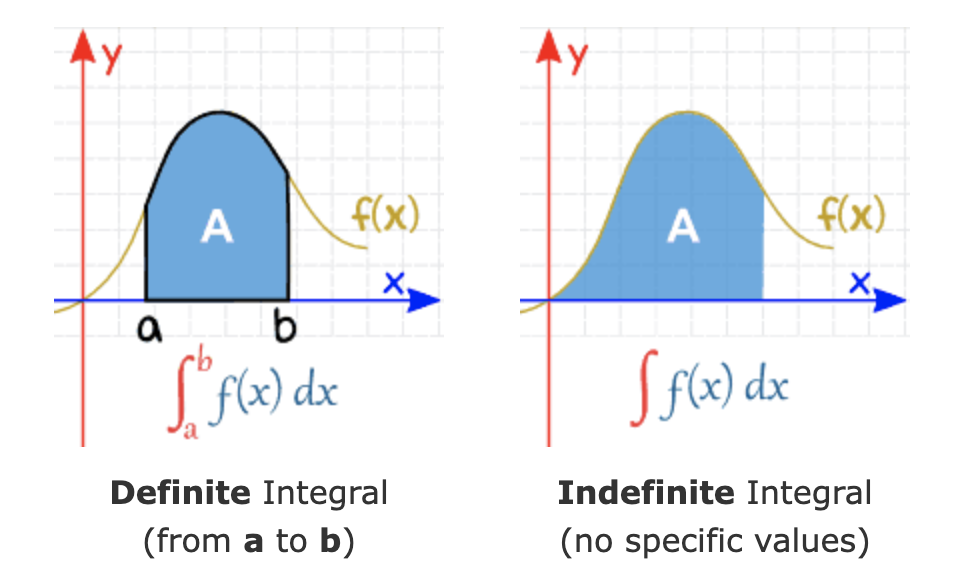
\includegraphics[width=0.5\linewidth]{topic03/Definite-Indefite} \end{center}

Let \(F(x) = \int_{-\infty}^x f(t) dt\), then definite integral \(\int_a^b f(t)dt = F(b) - F(a)\). This is called the \textbf{Fundamental Theorem of Calculus}. It is used to calculate the definite integral for a given function and the two integral limits.

\hfill\break

\textbf{Some Properties and Rules of Integrals}

\begin{enumerate}
\def\labelenumi{\arabic{enumi}.}
\item
  \(\int_a^b [f(x) \pm g(x)]dx = \int_a^b f(x)dx \pm \int_a^b g(x)dx\)
\item
  \(\int_a^b f(x)dx = -\int_b^a f(x) dx\)
\item
  \(\int_a^b f(x)dx = \int_a^c f(x)dx + \int_c^b f(x)dx\) for any constant \(c\) (\(c\) is not necessarily between \(a\) and \(b\)).
\end{enumerate}

\hfill\break

\hypertarget{practice-exercises-3}{%
\subsection{Practice Exercises}\label{practice-exercises-3}}

There two set of exercises you can practice. Ignore all problems involves trigonometric functions.

\begin{enumerate}
\def\labelenumi{\arabic{enumi}.}
\item
  Exercises with answer keys. \url{https://github.com/pengdsci/WCUSTA504/raw/main/topic03/Basic-Integration-Problems.pdf}
\item
  Worksheets: \url{https://pengdsci.github.io/WCUSTA504/Worksheet\%20Bundle.pdf}
\end{enumerate}

\begin{itemize}
\item
  Worksheet \#20: Fundamental Theorem of Calculus.
\item
  Worksheet \#21: Definite Integrals
\end{itemize}

\hfill\break

\hfill\break

\hypertarget{mixture-distributions}{%
\chapter{Mixture Distributions}\label{mixture-distributions}}

\emph{(Expanded from Section 4.11)}

We have outlined both discrete and continuous probability distributions and a few special families of distributions. In practical situations, single well-known distribution may not be able to characterize certain distributions well. For example, the log of income is usually considered to be log-normally distributed. According to \emph{the National Association of Colleges and Employers}, a survey of 563,000 recent college grads finds the gender pay gap already impacting the class of 2020.

\begin{center}\includegraphics[width=0.5\linewidth]{topic04/sallaryGapGender} \end{center}

Assume that the log salaries of each of the three categories follow a normal distribution. The overall distribution of the mixture of the three distributions may not be a normal distribution. The general shape of a mixture density could be the following form.

\begin{center}\includegraphics[width=0.6\linewidth]{topic04/mixtureDensityCurve} \end{center}

\hfill\break

\hypertarget{definition-of-mixture-model}{%
\section{Definition of Mixture Model}\label{definition-of-mixture-model}}

The idea is to find the density function of a population that contains several sub-populations with different probability distributions. Recall that a function \(f(x)\) is a density function of random variable \(X\) \texttt{if\ and\ only\ if}

\begin{enumerate}
\def\labelenumi{\arabic{enumi}.}
\item
  \(f(x) \ge 0\);
\item
  \(\int f(x) dx = 1.\)
\end{enumerate}

Before we introduce the formal definition of mixture mode, let's look at the following example.

\textbf{Example 1}: Starting salary of college graduates is an important factor in college ranking used by US News and Report. Assume that we are interested in the distribution of starting salary of WCU students. There are about 20\% are graduate students. Since the pay scales are different between graduate and undergraduate students. Therefore, the starting salary of undergraduate students is different from that of graduate students. Let \(X_1\) be the random variable representing the starting salary with density function \(f_(x)\) and \(X_2\) be the random variable representing the starting salary of graduate students with density function \(f_2(x)\). Now let \(X\) be the random variable representing the starting of all WCU graduates with density \(f(x)\), the density function can be defined as
\[
f(x) = (1-0.8)f_1(x) + 0.2f_2(x)
\]
We can check that \(f(x)\) is a valid density function in the following:

\begin{enumerate}
\def\labelenumi{\arabic{enumi}.}
\item
  Since \(f_1(x) \ge 0\) and \(f_2(x) \ge 0\), therefore, \(f(x) = 0.8f_1(x) + 0.2f_2(x) \ge 0\);
\item
  Note that \(\int f_1(x) = 1\) and \(\int f_2(x) = 1\). Therefore, \(\int f(x) = \int [0.8 f_1(x) + 0.2f_2(x)]\) \(= 0.8\int f_1(x) + 0.2 \int f_2(x) = 0.8\times 1 + 0.2 \times 1 = 1.0\)
\end{enumerate}

\emph{\textbf{Remarks}. Here are several remarks about the mixture distribution.}

\begin{enumerate}
\def\labelenumi{\arabic{enumi}.}
\item
  \emph{Unlike in the above example, we know the proportion of the graduate student population which is 20\%. In general, the proportion of sub-populations may not be known in practice. In this case, the proportion is considered as a population parameter that can be estimated from the sample. For example, we assume the graduate population to be \(\alpha\), then the undergraduate proportion is \(1-\alpha\). The above density function can then be written as \(f(x) = (1-\alpha)f_1(x) + \alpha f_2(x)\). In other words, \textbf{the density function of a mixture distribution is equal to the weighted average of the density functions of the sub-populations}}.
\item
  \emph{The density of the weighted average of random variable \((1-\alpha)X_1 + \alpha X_2\) is \textbf{NOT} \((1-\alpha)f_1(x) + \alpha f_2(x)\). We will discuss the distribution of the linear combination of }independent* random variables later this semester.*
\item
  \emph{We can also replace the density functions with the corresponding cumulative distributions (CDF) in the above definition of the mixture distribution.}
\end{enumerate}

\hypertarget{definition-of-k-component-mixture-distributions}{%
\subsection{Definition of K-component Mixture Distributions}\label{definition-of-k-component-mixture-distributions}}

The following is the definition of a k-component mixture distribution.

\textbf{Definition}: Let \(f_1(x), f_2(x), \cdots, f_k(x)\) be the density functions of k sub-populations. The density function of the mixture of these sub-populations is given by
\[
f(x) = p_1f_1(x) + p_2f_2(x) + \cdots + p_kf_k(x)
\]
where \(p_1, p_2, \cdots, p_k\) (\(0 \le p_i\le 1\)) are the corresponding proportions in the mixture of k sub-populations with \(p_1 +p_2 + \cdots + p_k = 1\).

\emph{\textbf{Remarks}: Since the above definition involves finite sub-populations, we it \textbf{finite mixture} distribution. There are mixture distributions that may involve infinite sub-populations or even uncountably infinite sub-populations (e.g., compound distribution). The finite mixture model is commonly used in practice.}

\hypertarget{properties-of-finite-mixture-distributions}{%
\subsection{Properties of Finite Mixture Distributions}\label{properties-of-finite-mixture-distributions}}

In previous notes, we introduced the steps for characterizing the distribution of a random variable:

\begin{enumerate}
\def\labelenumi{\arabic{enumi}.}
\item
  Explicitly define the random variable;
\item
  Define the probability distribution (i.e., specified distribution functions such as density or mass functions);
\item
  Provide formulas to calculate the key numerical characteristics such as mean, variance, etc. More generally, provide formulas to calculate moments of the distribution.
\end{enumerate}

\hfill\break

Recall also that the expectation of a single continuous variable with density function \(f(x)\) is defined in the following form

\[
E[X] = \int_{-\infty}^\infty xf(x)dx
\]
If the random variable is discrete with probability distribution function \(P(X = x)\), then expectation of \(X\) is then defined to be

\[
E[X] = \sum_{x}xP(X = x)
\]

In \textbf{Example 1}, we have explicitly defined the random variable that and the associated density function. We did not discuss the expectation and variance, etc. Next, we introduce a property of a general moment of mixture distributions.

\textbf{Property 1}: Let \(X_1, X_2, \cdots, X_k\) denote random variables from the \(k\)-component distributions, and let X denote a random variable from the mixture distribution. Then, for any function \(h(\cdot)\) for which \(E[h(X_i)]\) exists, and assuming that the component densities \(f_i(x)\) exist, for \(i = 1, 2, \cdots, k\), then
\[
E[h(X)] = \int_{-\infty}^\infty h(x)\sum_{i=1}^k p_i f_i(x) dx = \sum_{i=1}^k p_i\int_{-\infty}^\infty h(x)f_i(x) dx = \sum_{i=1}^k p_i E[h(X_i)]
\]

\textbf{k-th Moment}: Let \(X\) be a random variable with density function \(f(x)\), the \emph{k-th} of \(X\) is defined to be
\[
\mu^k = \int_{-\infty}^\infty x^k f(x) dx
\]

The first moment of the expectation. The variance \(E[(X-\mu)^2] = E[X^2] - \mu^2\), the difference between the 2nd moment and the square of the first moment.

\hfill\break

\textbf{Example 2}: Let \(X\) be the mixture distribution of two uniform distributions \(U_1(0, 10)\) and \(U_2(8, 14)\) with mixing proportions \(p_1\) and \(p_2\) respectively. Clearly, the two uniform density functions are given by

\[
f(x) = \left\{\begin{aligned}
& 1/(10-1), & x \in (0,10)\\
&0, &  x \notin (0,10)
\end{aligned},
\right.
\]
and
\[
f(x) = \left\{\begin{aligned}
& 1/(14-8), & x \in (8,14)\\
&0, &  x \notin (8,14)
\end{aligned}.
\right.
\]
The expectations of the two uniform distributions are \(\mu_1 = (10 + 0)/2 = 5\) and \(\mu_2 = (8 + 14) / 2 = 11\).

Now using the above property, we have
\[
E[X] = \int_{-\infty}^\infty xf(x)dx = \int_{-\infty}^\infty x[p_1f_1(x) + p_2f_2(x)]dx \\ = p_1\int_{-\infty}^\infty xf_1(x)dx + p_2\int_{-\infty}^\infty xf_2(x)dx = p_1\mu_1 +p_2\mu_2 = 5p_1 + 11p_2.
\]
since \(p_1 + p_2 = 1\).

With a closer look at the above formula of expectation, we can see that expectation of the mixture distribution is equal to the weighted average of expectations of the sub-populations. That is, it is the expected mean (``expectation of sub-population means'') if we consider the sub-population mean as a random variable with mixing proportions as their corresponding probabilities.

To be more specific, we can define a new random variable \(Y\) with the following probability distribution table

\begin{longtable}[]{@{}cc@{}}
\toprule\noalign{}
RV (Y) & P(\(Y=y\)) \\
\midrule\noalign{}
\endhead
\bottomrule\noalign{}
\endlastfoot
\(E[X|Y=1] = E[X_1] = \mu_1 = 5\) & \(p_1\) \\
\(E[X|Y=2] = E[X_2] = \mu_2 = 11\) & \(p_2\) \\
\end{longtable}

Using the above probability distribution of \(Y\), we can then rewrite the expectation of the mixture distribution as

\[
E_X[X]  = p_1\mu_1 +p_2\mu_2 = p_1E[X|Y=1] + p_2E[X|Y=2] \stackrel{def}{=} E_Y(E_X[X|Y]).
\]

This leads to the definition of conditional expectation in the following. Let \(X\) and \(Y\) be two random variables. Assume that \(X\) is a continuous variable, the density of \(X\) conditioning on \(Y\) is \(f(x|Y)\). The \textbf{conditional expectation} of \(X|Y\) (\emph{reads \(X\) conditioning on \(Y\)}) is given by

\[
E[X|Y] = E_X[X|Y] = \int_{-\infty}^\infty xf(x|Y)dx.
\]

Obviously, \(E[X|Y]\) is random because \(Y\) is random. In finite mixture distribution, \(Y\) represents the subpopulation. Therefore, the expectation of the overall mixture distribution is

\[
E_X[X] = E_X[E_Y(X|Y)] = p_1\int_{-\infty}^\infty xf(x|Y=1)dx + p_2 \int_{-\infty}^\infty xf(x|Y=2)dx \\ = p_1\mu_1 + p_2\mu_2.
\]

The above equation is correct in general for any two random variables.

\textbf{Property 2}: \emph{Conditional Expectation} For \emph{any} given random variables \(X\) and \(Y\), the following property holds
\[
E_X[X] = E_X[E_Y(X|Y)] .
\]

\hfill\break

\hypertarget{variance-decomposition}{%
\subsection{Variance Decomposition}\label{variance-decomposition}}

We have introduced conditional expectation and its property. In this section, we introduce the variance decomposition formula using conditional expectation. We will also use these formulas in later chapters of this course.

We have expressed the overall expectation of the mixture distribution in terms of the expectations of individual subpopulations. A natural question is whether the variance can be decomposed into the variances of individual subpopulations.

The following variance decomposition property answers the question.

\textbf{Property 3}: \emph{Variance Decomposition}: Let \(X\) and \(Y\) be two random variables. Then
\[
Var[X] = E[Var(X|Y)] + Var[E(X|Y)
\]
\textbf{Proof}: First of all, we note that \(Var[X] = E(X - E[X])^2 = E[X^2] - (E[X])^2\).
This implies that
\[
Var(X|Y) = E(X^2|Y) - [E(X|Y)]^2
\]
Similar to the conditional expectation, the conditional variance is also a random variable. Therefore,

\[
\begin{aligned}
E_Y[Var(X|Y)] & =E_Y[E(X^2|Y)] - E_Y\{ [E(X|Y)]^2\} &\\
     & = E[X^2] - E_Y\{ [E(X|Y)]^2\} &\\
     & = \{E[X^2] - (E[X])^2 \} - \{ E_Y\{ [E(X|Y)]^2\} - (E[X])^2 \}\} &\\
     & = Var[X] - \{ E_Y\{ [E(X|Y)]^2\} - \{E_Y[E(X|Y)]\}^2 \} &\\
     & = Var[X] - Var_Y[E_X(X|Y)]
\end{aligned}
\]
Moving the terms around, we have
\[
Var[X] = E_Y[Var(X|Y)] + Var_Y[E_X(X|Y)]
\]
This completes the proof.

\emph{\textbf{Remark}: The right hand of the variance decomposition formula only involves the conditional random variable. We can express the right-hand formula in terms of individual variances, expectations, and mixing proportions.}

\hfill\break

\textbf{Example 3}. Let \(X\) be the mixture distribution defined based on two distributions with density functions \(f_1(x)\) and \(f_2(x)\). Assume the expectation and the variance of the two subpopulations are \((\mu_1, \sigma_1^2)\) and \((\mu_2, \sigma_2^2)\) respectively. Assume further that the mixing proportions are \(p_1\) and \(p_2\) with \(p_1 + p_2 = 1\). Find the variance of the mixture distribution Var{[}X{]}.

\textbf{Solution}: We two different methods to find the variance.

\emph{\textbf{Method 1:} Using the variance decomposition formula.}

By the definition of expectation and variance, we obtain the two terms on the right side of the formula in the following.
\[
\begin{aligned}
E_Y[Var(X|Y)] & = p_1\sigma_1^2 + p_2\sigma_2^2  &\\
\end{aligned}
\]
Note that \(E\{E[X|Y]\} = p_1\mu_1 + p_2\mu_2\). Therefore,

\[
\begin{aligned}
Var_Y[E(X|Y)] & =  E_Y\{E(X|Y) - E_Y[E(X|Y)]\}^2  &\\
              & =  E_Y\{E(X|Y) - (p_1\mu_1 + p_2\mu_2)\}^2  &\\
              & =  p_1(\mu_1-p_1\mu_1-p_2\mu_2)^2 + p_2(\mu_2-p_1\mu_1-p_2\mu_2)^2 &\\
              & =  p_1[\mu_1^2 -2\mu_1 (p_1\mu_1+p_2\mu_2) + (p_1\mu_1+p_2\mu_2)^2]   &\\
              &   + p_2[\mu_2^2 -2\mu_2 (p_1\mu_1+p_2\mu_2) + (p_1\mu_1+p_2\mu_2)^2] &\\
              & = p_1\mu_1^2 + p_2\mu_2^2 -2(p_1\mu_2+p_2\mu_2)^2 + (p_1+p_2)(p_1\mu_2+p_2\mu_2)^2 &\\
              & = p_1\mu_1^2 + p_2\mu_2^2 -(p_1\mu_2+p_2\mu_2)^2.
\end{aligned}
\]
Therefore,

\[
Var[X] =  p_1\sigma_1^2 + p_2\sigma_2^2  + p_1\mu_1^2 + p_2\mu_2^2 -(p_1\mu_2+p_2\mu_2)^2.
\]\\

\textbf{Method 2}: Using the moment formula and the relation \(Var[X] = E[X^2] - (E[X])^2\).
Note that \(E[X] = p_1\mu_1 + p_2\mu_2\). From \emph{Property 1}, we can find the 2nd moment of \(X\) in the following
\[
E[X^2] = p_1\mu_1^{(2)} + p_2\mu_2^{(2)}
\]
where \(\mu_1^{(2)}\) and \(\mu_2^{(2)}\) are the 2nd moment of the individual sub-populations which can be expressed in terms of the individual means and variance as follows
\[
\mu_1^{(2)} = \sigma_1^2 + \mu_1^2 \mbox{ and } \mu_2^{(2)} = \sigma_2^2 + \mu_2^2
\]
With the above facts, we have
\[
E[X^2] = p_1(\sigma_1^2 + \mu_1^2) + p_2(\sigma_2^2 + \mu_2^2)
\]
Therefore,

\[
Var[X]   = p_1(\sigma_1^2 + \mu_1^2) + p_2(\sigma_2^2 + \mu_2^2) - ( p_1\mu_1 + p_2\mu_2)^2,
\]
which is identical to the result obtained in \emph{Method 1}.

\hfill\break

\hypertarget{two-component-normal-mixture-distribution}{%
\section{Two-component Normal Mixture Distribution}\label{two-component-normal-mixture-distribution}}

Let \(X_1\) and \(X_2\) be two normal distributions with distributions \(N_1(\mu_1, \sigma_1)\) and \(N_2(\mu_2, \sigma_2)\), respectively and \(X\) be the random variable representing the mixture distribution of the two normal populations with proportions \(p_1\) and \(p_2\) respectively.

The explicit expression of the mixture density function is given by
\[
f(x) = \frac{p_1}{\sqrt{2\pi}\sigma_1}e^{-\frac{(x-\mu_1)}{2\sigma_1^2}} +  \frac{p_2}{\sqrt{2\pi}\sigma_2}e^{-\frac{(x-\mu_2)}{2\sigma_2^2}}
\]

The expectation and variance in \textbf{Example 4} apply to this two-component normal mixture distribution.

\textbf{Some Special Cases}: In general, the mixture distribution of finite normal distribution is NOT a normal distribution. Next, we use the two-component normal mixture distribution as an example to show that a finite normal mixture can be a normal distribution only in some special cases.

\begin{enumerate}
\def\labelenumi{\arabic{enumi}.}
\item
  For a two-component normal mixture distribution, if one of the mixing proportions is zero (i.e., \(p_1 = 0\) or \(p_2 = 0\)), then the resulting mixture is a normal distribution.
\item
  If \(\mu_=\mu_2\) and \(\sigma_1 = \sigma_2\), then the resulting mixture is also a normal distribution.
\end{enumerate}

The following figure shows the general two-component normal mixture.

\hfill\break

\begin{center}\includegraphics[width=0.5\linewidth]{topic04/twoComponentGaussianMixture} \end{center}

The above figure is based on simulated data from \(N_1(\mu_1, \sigma) = N_1(-2.8, 0.48)\) and \(N_2(\mu_2, \sigma_2) = N_2(1.86, 0.88)\) with mixing proportion \(p_1 = 0.4\) and \(p_2 = 0.6\), respectively.

\hfill\break

\hypertarget{use-mixture-distributions}{%
\section{Use Mixture Distributions}\label{use-mixture-distributions}}

Mixture distributions are widely used in both classical statistics and modern machine learning areas.

\hypertarget{fitting-complex-data-using-mixture-distributions}{%
\subsection{Fitting Complex Data Using Mixture Distributions}\label{fitting-complex-data-using-mixture-distributions}}

In real-world applications, it is quite often that a single well-established distribution does not fit the data with a complex structure. In this case, we may use mixture distributions to characterize the complex pattern.

\textbf{Example 5}: Pearson fit a mixture of two normal distributions to Naples' crab data (1989). The hypothesis was that the data was in fact a mixture of two different species of crabs. Although the empirical data histogram is single-peaked, the mixture of two normal produced a better fit.

(\emph{Source: K. Pearson: Contributions to the Mathematical Theory of Evolution. Philosophical Transactions of the Royal Society of London. A, 1894.})

The following figure shows the histogram and actually fitted density curve of the two-component normal mixture distribution.

\begin{center}\includegraphics[width=0.5\linewidth]{topic04/PearsonCrabData} \end{center}

\hypertarget{clustering-with-mixture-distributions}{%
\subsection{Clustering with Mixture Distributions}\label{clustering-with-mixture-distributions}}

Clustering analysis is one of the most important tasks in both classical statistics and modern machine learning. There are many well-established algorithms for clustering. Mixture model-based clustering is a statistical-based method that has a solid theoretical base. It is one of the most powerful unsupervised machine learning algorithms.

One of the questions in many applications is to find data points that have \emph{some sort of similarity} and then cluster them to define several groups to reduce variations in modeling. One task in clustering is to decide the optimal number of clusters to group the data. Too many groups and too few groups will increase the heterogeneity of the data when modeling. This means when using mixture distribution, the number of mixture components needs to be determined. We can use goodness-of-fit metrics to determine the appropriate number of mixing components.

The following figure shows an empirical distribution (the black unsmooth curve). Three candidate mixture distributions were fit to the data.

\begin{center}\includegraphics[width=1\linewidth]{topic04/Clustering} \end{center}

We can see that the leftmost figure shows the fit of a two-component normal mixture, the middle figure represents a three-component normal mixture and the right-hand side is a four-component normal mixture distribution. It turns out the three-component normal mixture has the best fit.

\hfill\break

\hfill\break

\hypertarget{moment-generating-functions-mgf}{%
\chapter{Moment Generating Functions (MGF)}\label{moment-generating-functions-mgf}}

\textbf{Moment generating functions (MGF)} are useful for several reasons, one of which is their application to the analysis of sums of random variables such as sample means to make inferences of a population mean. The other application of MGF is to develop methods for estimating population parameters. From the theoretical perspective, it can be used to completely characterize the distribution of random variables. In this note, we briefly introduce the concepts of MGF and derive the MGF of some of the basic distributions.

\hypertarget{moments-of-rv-and-mgf}{%
\section{Moments of RV and MGF}\label{moments-of-rv-and-mgf}}

We have defined the k-th moment of a random variable \(Y\) with a distribution function. There are different moments we can define for a random variable. We first briefly review these moments and then define the MGF.

\hypertarget{various-moments-revisited}{%
\subsection{Various Moments Revisited}\label{various-moments-revisited}}

Recall that the k-th moment of a random variable is defined to be of the following form

\[
\displaystyle E[Y^k] = \begin{cases} 
 \int_{-\infty}^{\infty} y^k f(y)dy & \text{if $y$ is continuous}, \\  
 \sum_y y^kP(Y=y) & \text{otherwise}.
 \end{cases}
\]

where \(f(y)\) and \(P(Y=y)\) are probability density function and probability distribution function (probability mass function) respectively.

The k-th central moment of \(Y\) is defined to be

\[
\displaystyle E[(Y-\mu)^k] = \begin{cases} 
 \int_{-\infty}^{\infty} (y-\mu)^k f(y)dy & \text{if y is continuous}, \\  
 \sum_y (y-\mu)^kP(Y=y) & \text{otherwise}.
 \end{cases}
\]

where \(\mu = E[Y]\). As a special case, when \(k=2\), the second central moment \(E[(Y-E[Y])^2]\) is the variance of \(Y\).

In general, if \(g(Y)\) is a function of random variable \(Y\), then we have the general expectation in the following form

\[
\displaystyle E[g(Y)] = \begin{cases} 
 \int_{-\infty}^{\infty} g(y) f(y)dy & \text{if y is continuous}, \\  
 \sum_y g(y)P(Y=y) & \text{otherwise}.
 \end{cases}
\]

\hypertarget{mgf}{%
\subsection{MGF}\label{mgf}}

The MGF is a special case of the expectation of a function of a random variable. Let \(Y\) be a random variable with density \(f(y)\) (if \(Y\) is continuous) or \(P(Y=y)\) (if \(Y\) is discrete). Then the moment generating function of \(Y\) is defined to be

\[
\displaystyle m_Y(t) = E[e^{tY}] = \begin{cases} 
 \int_{-\infty}^{\infty} e^{ty} f(y)dy & \text{if $y$ is continuous}, \\  
 \sum_y e^{ty}P(Y=y) & \text{otherwise}.
 \end{cases}
\]

MGF of \(Y\) is a function of \(t\) (\(t\) is any real number).

\hfill\break

\hypertarget{properties-of-mgf}{%
\section{Properties of MGF}\label{properties-of-mgf}}

To study MGF, we need some basic concepts of series and Taylor expansion.

\hypertarget{review-of-taylor-series}{%
\subsection{Review of Taylor Series}\label{review-of-taylor-series}}

In mathematics, it is common in many situations in which we use (mathematically) simple functions to approximate complicated mathematical functions. The well-known Taylor expansion is such an example.

The general Taylor expansion of a function \(f(x)\) at a given value \(x_0\) is given by

\[
f(x) = f(x_0) + f^{(1)}(x_0)(x-x_0) + \frac{f^{(2)}(x_0)}{2!}(x-x_0)^2 
\]

\[
+ \frac{f^{(3)}(x_0)}{3!}(x-x_0)^3 + \cdots + \frac{f^{(n)}(x_0)}{n!}(x-x_0)^n +\cdots 
\]

Note that the right-hand side of the above expansion is a polynomial with infinite degrees. If we keep only finite terms and drop the rest of the higher order terms, we will obtain the approximation of \(f(x)\).

\[
f(x) \approx f(x_0) + f^{(1)}(x_0)(x-x_0) + \frac{f^{(2)}(x_0)}{2!}(x-x_0)^2
\]

\[
+ \frac{f^{(3)}(x_0)}{3!}(x-x_0)^3 + \cdots + \frac{f^{(n)}(x_0)}{n!}(x-x_0)^n 
\]

\textbf{Example 1}. Let \(f(x) = \sqrt{x}\). Find the Taylor expansion of \(f(x)\) at \(x = 1\).

\textbf{Solution}: Note that \(\sqrt{x} = x^{1/2}\), we use the power rule of derivative repeatedly to expand \(f(x)\). For convenience, I list the first few high-order derivatives of \(\sqrt{x}\) in the following

\[
[\sqrt{x}]^{(1)} = \frac{1}{2}x^{1-1/2} = \frac{1}{2}x^{-1/2}
\]

\[
[\sqrt{x}]^{(2)} =  [\frac{1}{2}x^{-1/2}]^\prime = \frac{1}{2}(-\frac{1}{2})x^{-1/2-1} = -\frac{1}{4}x^{-3/2}
\]

\[
[\sqrt{x}]^{(3)} = [-\frac{1}{4}x^{-3/2}]^\prime =-\frac{1}{4}(-\frac{3}{2})x^{-3/2-1} = \frac{3}{8}x^{-5/2}
\]

\[
[\sqrt{x}]^{(4)}  = [\frac{3}{8}x^{-5/2}]^\prime = \frac{3}{8}(-\frac{5}{2})x^{-5/2-1} = -\frac{15}{16}x^{-7/2}
\]

By the above Taylor expansion formula, we write the first few terms of the expansion in the following

\[
\sqrt{x} = \sqrt{1} + \frac{\frac{1}{2}x^{-1/2}|_{x=1}}{1!}(x-1) + \frac{-\frac{1}{4}x^{-3/2}|_{x=1}}{2!}(x-1)^2 
\]

\[
+ \frac{\frac{3}{8}x^{-5/2}|_{x=1}}{3!}(x-1)^3 + \frac{-\frac{15}{16}x^{-7/2}|_{x=1}}{4!}(x-1)^4 + \cdots 
\]

\[
=\sqrt{1} +\frac{1}{2}(x-1) - \frac{1}{8}(x-1)^2 + \frac{1}{16}(x-1)^3 - \frac{5}{128}(x-1)^4 +\cdots
\]

\textbf{Example 2}: Let \(f(x) = e^x\). Expand \(f(x)\) at \(x = 0\).

\textbf{Solution}: Since the derivative of the natural base exponential \(f(x) = e^x\) is equal to itself. In other words, \(f^{(n)}(x) = [e^x]^{(n)} = e^x\). The Taylor expansion of \(e^x\) is given below.

\[
f(x) = e^0 + \frac{e^0}{1!}x + \frac{e^0}{2!}x^2+\frac{e^0}{3!}x^3 + \frac{e^0}{4!}x^4 + \cdots
\]

\[
= 1 + x + \frac{x^2}{2!} + \frac{x^3}{3!} + \frac{x^4}{4!} + \frac{x^5}{5!}  +\cdots
\]

\hypertarget{how-mgf-generates-moments}{%
\subsection{How MGF Generates Moments?}\label{how-mgf-generates-moments}}

Next, we show how MGF generates moments. Note that the MGF is the expectation of random variable \(e^{tY}\) (t is the regular variable and \(Y\) is a random variable with density function \(f(y)\)). We first expand the \textbf{random} function \(e^{tY}\) (as a function of \(t\)) at \(t = 0\) by noting that

\[
[e^{tY}]^{(1)} = \frac{d e^{tY}}{dt} = Ye^{tY} 
\]

\[
[e^{tY}]^{(2)}  = \frac{d (Ye^{tY})}{dt} = Y^2e^{tY}
\]

\[
[e^{tY}]^{(3)}  = \frac{d (Y^2e^{tY})}{dt} = Y^3e^{tY} 
\]

\[
\cdots \cdots \cdots \cdots \cdots \cdots
\]

\[
e^{tY} = e^0 + \frac{Ye^{0\times Y}}{1!}(t-0) + \frac{Y^2e^{0\times Y}}{2!}(t-0)^2 + \frac{Y^3e^{0\times Y}}{3!}(t-0)^3 + \cdots \\ = 1 + Yt + \frac{Y^2}{2!}t^2 + \frac{Y^3}{3!}t^3 + \cdots
\]

The MGF is defined by

\[
m_Y(t) = E[e^{tY}]=E[1 + Yt + \frac{Y^2}{2!}t^2 + \frac{Y^3}{3!}t^3 + \cdots] \\ = 1 + tE[Y] + \frac{t^2}{2!}E[Y^2] + \frac{t^3}{3!}E[Y^3] + \cdots
\]

We can see from the above expression that the coefficients of MGF contain moments. Next, we find the first few moments of Y based on \(m_Y(t)\).

\[
[m_Y(0)]^{(1)}=\frac{d[m_Y(t)]}{dt}|_{t=0} = [1 + tE[Y] + \frac{t^2}{2!}E[Y^2] + \frac{t^3}{3!}E[Y^3] + \cdots]^\prime_{t=0} \\
= [E[Y] + tE[Y^2] + \frac{t^2}{2!}E[Y^3] + \cdots]_{t=0} = E[Y]
\]

We keep taking derivatives and evaluate them at \(t = 0\) to obtain other moments. In general,

\[
[m_Y(0)]^{(k)} = E[Y^k]
\]

\hypertarget{mgf-of-some-special-distributions}{%
\section{MGF of Some Special Distributions}\label{mgf-of-some-special-distributions}}

In this section, we find MGFs of several well-known distributions.

\hypertarget{exponential-distribution}{%
\subsection{Exponential Distribution}\label{exponential-distribution}}

Let \(X\) be a random variable with the following density function

\[
\displaystyle f(y) = \begin{cases} 
 \lambda e^{-\lambda y} & \text{if $y \ge 0$}, \\  
 0 & \text{otherwise}.
 \end{cases}
\]

The moment generating function is given by

\[
m_Y(t) = E[e^{tY}] = \int_0^\infty e^{ty} \lambda e^{-\lambda y}dy = \int_0^\infty \lambda e^{-(\lambda-t)y}dy
\]

\[
=\frac{\lambda}{\lambda -t}\int_0^\infty (\lambda -t)e^{-(\lambda-t)y}dy = \frac{\lambda}{\lambda -t}
\]

\hypertarget{normal-distribution-1}{%
\subsection{Normal Distribution}\label{normal-distribution-1}}

The moment generating function (MGF) for the standard normal random variable with density function.

\[
f(x) = \frac{1}{\sqrt{2\pi}}e^{-\frac{x^2}{2}}
\]

By the definition,

\[
m_Y(t) = E[e^{tY}] = \int_{-\infty}^\infty e^{ty} \frac{1}{\sqrt{2\pi}}e^{-\frac{y^2}{2}}dy =\int_{-\infty}^\infty \frac{1}{\sqrt{2\pi}}e^{-\frac{x^2}{2}+ty}dy
\]

\[
=\int_{-\infty}^\infty \frac{1}{\sqrt{2\pi}}e^{-\frac{y^2-2ty}{2}}dy = \int_{-\infty}^\infty \frac{1}{\sqrt{2\pi}}e^{-\frac{y^2-2ty+t^2 - t^2}{2}}dy
\]

\[
= e^{\frac{t^2}{2}}\int_{-\infty}^\infty \frac{1}{\sqrt{2\pi}}e^{-\frac{y^2-2ty+t^2}{2}}dy = e^{\frac{t^2}{2}}\int_{-\infty}^\infty \frac{1}{\sqrt{2\pi}}e^{-\frac{(y-t)^2}{2}}d(y-t) = e^{\frac{t^2}{2}}
\]\\

\hfill\break

\hypertarget{use-of-mgf---shape-analysis}{%
\section{Use of MGF - Shape Analysis}\label{use-of-mgf---shape-analysis}}

\textbf{Shape analysis} of distribution plays an important role in many applications such as quality control, process monitoring, reliability modeling, etc. Skewness and kurtosis are the two most commonly used metrics in shape analysis. They are defined based on the moments of standardized random variable \((Y-\mu)/\sigma\), where \(\mu = E[Y]\) and \(\sigma = \sqrt{E(Y-\mu)^2}\). In this section, we define both metrics at the population level. In data analysis, we can convert these metrics to their corresponding sample versions to assess the skewness and kurtosis of the data.

\hypertarget{skewness}{%
\subsection{Skewness}\label{skewness}}

\textbf{Skewness} is a measure of symmetry, or more precisely, the lack of symmetry. A distribution, or data set, is symmetric if it looks the same to the left and right of the center point. The exact definition is given by

\[
Skew(Y) = E\left[ \left(\frac{Y-\mu}{\sigma}\right)^3\right]=\frac{E[Y^3] -3\mu E[Y^2] + 3\mu^2 E[Y]-\mu^3}{\sigma^3}
\].

\begin{itemize}
\item
  Negative skew indicates that the tail is on the left side of the distribution, which extends towards more negative values.
\item
  Positive skew indicates that the tail is on the right side of the distribution, which extends towards more positive values.
\item
  A value of zero indicates that there is no skewness in the distribution at all, meaning the distribution is perfectly symmetrical.
\end{itemize}

\begin{center}\includegraphics[width=0.7\linewidth]{topic05/skewness} \end{center}

\textbf{Example 3}: Use the method of finding moments from MGF (Section 3.2 of this note) to find the skewness of the standard normal distribution.

\textbf{Solution}: For the standard normal distribution (denoted by \(Z\)), \(\mu =0\) and \(\sigma =1\). The skewness of the standard normal distribution is reduced to

\[
Skew(Z) = E[Y^3]
\]

Next, we take the third order derivative of its moment generating function \(m_Z(t) = e^{-t^2/2}\) introduced in 4.2 and evaluate the result at 0 to get the third moment.

\[
\frac{d m_Z(t)}{dt} =te^{t^2/2},  \frac{d^2 m_Z(t)}{dt^2} =\frac{d(te^{t^2/2})}{dt}=(t^2+1)e^{t^2/2}
\]

\[
\frac{d^3 m_Z(t)}{dt^3} =\frac{d[(t^2+1)e^{t^2/2}]}{dt} = [2t+t(t^2+1)]e^{t^2/2} = t(t^2+3)e^{t^2/2}
\]

Therefore, for the standard normal distribution

\[
skew(Z) = E[Z^3] = \frac{d^3 m_Z(0)}{dt^3} = t(t^2+3)e^{t^2/2}|_{t = 0} = 0.
\]

This confirms the symmetry of the standard normal distribution.

\hypertarget{kurtosis}{%
\subsection{Kurtosis}\label{kurtosis}}

\textbf{Kurtosis} is a measure of whether the distributions are heavy-tailed or light-tailed relative to a normal distribution. That is, distributions with high kurtosis tend to have heavy tails, or outliers relative to \textbf{normal distributions}. Distributions with low kurtosis tend to have light tails or lack outliers. A uniform distribution would be the extreme case.

\[
kurt(Y) = E\left[ \left(\frac{Y-\mu}{\sigma}\right)^4\right]=\frac{E[Y^4]-4\mu E[Y^3] + 6\mu^2E[Y^2]-3\mu^4}{\sigma^4}
\].

\begin{itemize}
\item
  The kurtosis of a normal distribution is 3 (see the following \textbf{Example 4}). When discussing kurtosis, we use normal distributions as a reference.
\item
  If a given distribution has a kurtosis less than 3, it is said to be playkurtic, which means it tends to produce fewer and less extreme outliers than the normal distribution.
\item
  If a given distribution has a kurtosis greater than 3, it is said to be leptokurtic, which means it tends to produce more outliers than the normal distribution.
\end{itemize}

\begin{center}\includegraphics[width=0.4\linewidth]{topic05/kurtosis} \end{center}

\hfill\break

\textbf{Example 4}: Find the kurtosis of the standard normal distribution.

\textbf{Solution}: Note that \(\mu = 0\) and \(\sigma = 1\) in the standard normal distribution. Therefore, the kurtosis of the standard normal distribution is reduced to

\[
Kurt(Z) = E[Y^4].
\]

Next, we continue the process in \textbf{example 3} to find the 4-th derivative of the MGF of Z.

\[
\frac{d^4 m_Z(t)}{dt^4} =\frac{d\{(3t+t^3)e^{t^2/2}\}}{dt} = [(3+3t^2)+t(3t+t^3)]e^{-t^2/2}=(t^4+6t^2+3)e^{t^2/2}
\]

Therefore, \(Kurt(Z) = E[Z^4] = \frac{d^4 m_Z(0)}{dt^4} = (t^4+6t^2+3)e^{t^2/2}|_{t=0} = 3\).

\hfill\break

\hypertarget{joint-distributions-and-marginal-distributions}{%
\chapter{Joint Distributions and Marginal Distributions}\label{joint-distributions-and-marginal-distributions}}

This note is dedicated to the joint and marginal distributions of multivariate variables. The primary emphasis will be the bivariate distributions (both continuous and discrete). \textbf{The first three sections of chapter 5} in the textbook cover these topics.

\hypertarget{joint-distribution-of-categorical-variables}{%
\section{Joint Distribution of Categorical Variables}\label{joint-distribution-of-categorical-variables}}

For ease of simplicity, we only discuss the joint distribution of two categorical variables. If both categorical variables are ordinal, we can encode labels and treat the encoded categorical variables as discrete numerical variables and use the same method to be discussed in the next section to define joint and cumulative distributions. But the numerical measures such as those associated with moments are NOT well defined.

Next, we use an example to illustrate the joint distribution of two categorical variables.

\textbf{Example 1}: If we want to know the relationship between the \textbf{attitude of life} and \textbf{marital status} by exploring the distribution of these two variables. We assume the following two-way contingency table was constructed based on a random sample from a population.

\begin{center}\includegraphics[width=0.4\linewidth]{topic06/twoNominalCateFreqTables} \end{center}

We can easily convert the above two-way contingency table to a joint probability distribution table in the following.

\begin{center}\includegraphics[width=0.55\linewidth]{topic06/twoNominalCateJointDistTables} \end{center}

We can define the joint probability distribution for a specific event based on the table

\[
p_{ij} = P[X= row \ number, Y = column \ number]
\]

Assume that \(X\) has \(I\) categories and \(Y\) has \(J\) categories. The following two requirements analogous to that required in univariate distributions are also satisfied.

\begin{enumerate}
\def\labelenumi{\arabic{enumi}.}
\item
  \(0 \le p_{ij} \le 1\) for \(1 \le i \le I\) and \(1 \le j \le J\).
\item
  \(\sum_{i=1}^I \sum_{j = 1}^J p_{ij} = 1.\)
\end{enumerate}

It is important to note that the cumulative probability distribution (CDF) of categorical variables is defined based on \textbf{ordered} categorical variables. Therefore, for nominal categorical variables, the CDF of the joint distribution is \textbf{NOT} defined.

We can define \textbf{bivariate} events using discrete sets. For example, \(E = \left[ X\in\{'Married',\ 'Never \ Married'\}\right] \cap \left[Y\in\{'Dull',\ 'Never \ Exciting'\} \right]\) is a bivariate event defined based on the distribution table in \textbf{Example 1} (see the following table with highlighted cells).

\begin{center}\includegraphics[width=0.55\linewidth]{topic06/twoNominalCateJointDistEventProb} \end{center}

We can easily find the probability of observing event \(E\)

\[
P(E) = 0.021 + 0.252 + 0.011 + 0.109 = 0.393.
\]

In general, a bivariate event is defined in the form of

\[
E = \bigr[ X\in \{ set \ of \ category \ labels \ of \ X\} \bigr]\bigcap \bigr[ Y\in \{ set \ of \ category \ labels \ of \ Y\} \bigr]
\]

The objective of studying the joint distribution of the categorical variables is to see whether they are independent of each other. For example, the well-known \(\chi^2\) test of independence was developed for this purpose. More details on the theory behind this test will be discussed in the next note.

In the next two sections, we discuss bivariate numerical distributions.

\hfill\break

\hypertarget{discrete-bivariate-distributions}{%
\section{Discrete Bivariate Distributions}\label{discrete-bivariate-distributions}}

Recall that the probability distribution of univariate random variable \(X\) (assuming \(X\) taking values \(\{x_1, x_2, \cdots, x_n, \cdots \}\)) can be graphically represented in the following.

\begin{center}\includegraphics[width=0.6\linewidth]{topic06/univariateDiscreteDist} \end{center}

that satisfies

\begin{enumerate}
\def\labelenumi{\arabic{enumi}.}
\item
  \(0 \le P(x_i) \le 1\) for \(i=1, 2, \cdots\)
\item
  \(\sum_i P(x_i) = 1\).
\end{enumerate}

We also note that the definition of expectation and variance are given by

\begin{itemize}
\item
  \(\mu = E[X] = \sum_i x_iP(X = x_i)\).
\item
  \(V[X] = \sum_i (x_i - \mu)^2P(X=x_i)\).
\end{itemize}

The cumulative distribution function (CDF) is defined to be

\[
P[X \le x] = \sum_{x_i \le x} P(X = x_i)
\]

\hypertarget{joint-distribution-and-properties}{%
\subsection{Joint Distribution and Properties}\label{joint-distribution-and-properties}}

For a bivariate distribution, we use the following example to demonstrate the definition of the joint distribution. Consider an experiment of rolling a six-sided \textbf{fair} dice and flipping an \textbf{imbalanced} coin. Let \(Y =\) the number of dots facing up when rolling a die and \(X =\) the outcome observed (\(X = 1\) if a Heads is observed and \(X = 2\) if a Tails is observed). Then the following two-way contingency table illustrates the joint distribution of random variables \(X\) and \(Y\).

\begin{center}\includegraphics[width=0.7\linewidth]{topic06/discreteBivariateJointDistTable} \end{center}

We can also use the following 3-D chart to represent the above joint distribution

\begin{center}\includegraphics[width=0.8\linewidth]{topic06/discreteBivariateDist} \end{center}

\textbf{Joint Probability}: The \emph{height} of each vertical bar that is equal to the corresponding cell of the contingency table represents the joint probability of observing the two corresponding values respectively. For example, \(P[X=2, Y =3] = 3/60\) (see the marked cell in the table and labeled bar in the figure).

The above table is called the \textbf{joint probability distribution table} of random variables \(X\) and \(Y\).

We can also call the above chart \textbf{joint probability distribution histogram}.

Similarly, we observe the following requirements that are analogous to the univariate distributions.

\begin{enumerate}
\def\labelenumi{\arabic{enumi}.}
\item
  \(0 \le P(X=x_i, Y=y_j) = p_{ij} \le 1\);
\item
  \(\sum_i\sum_j P(X=x_i, Y=y_j) = 1\).
\end{enumerate}

The \textbf{cumulative distribution function (CDF)} is defined to be of the following form

\[
F(x,y) = \sum_{x_i < x} \sum_{y_i < y} P(X=x_i, Y=y_i)
\]

The following figure shows how to calculate \(F(2,3)\).

\begin{center}\includegraphics[width=0.8\linewidth]{topic06/discreteBivariateCDF} \end{center}

The value of \(F(2,3)\) is equal to the sum of the heights of all vertical bars in the top-left corner of \(xy\)-plane. That is,

\[
F(2,3) = 3\times\frac{7}{60} + 3\times \frac{3}{60} = \frac{30}{60} = 0.5.
\]

Similarly, we can find \(F(1.5, 4.5) = 4\times (7/60) = 28/60 =7/15\).

\textbf{A Cautionary Note:} We have numerically encoded the outcome labels of the trial of flipping a coin (Heads = 1 and Tails = 2). The encoded values have a natural order. So we can define the CDF of using the standard form \(F(x,y) = P(X \le x, Y \le y )\) that involves \textbf{'}\(\le\)'

\hypertarget{marginal-distributions}{%
\subsection{Marginal Distributions}\label{marginal-distributions}}

Notice that row and column totals in the margins of the following joint probability distribution table satisfy the distribution of discrete univariate random variables. For this reason, we call the row totals the \textbf{marginal distribution} of \(X\), and the column totals the \textbf{marginal distribution} of \(Y\).

\begin{center}\includegraphics[width=0.8\linewidth]{topic06/discreteMarginalDistribution} \end{center}

Graphically, the marginal distribution histograms are given in the following figure.

\begin{center}\includegraphics[width=0.8\linewidth]{topic06/discreteBivariateMarginalDistGraph} \end{center}

\hfill\break

\hypertarget{continuous-bivariate-distributions}{%
\section{Continuous Bivariate Distributions}\label{continuous-bivariate-distributions}}

We can similarly generalize the univariate distribution to multivariate distribution. Recall that the probability density function (\emph{pdf}) \(f(x)\) of a continuous random variable meets the following two conditions.

\begin{enumerate}
\def\labelenumi{\arabic{enumi}.}
\item
  \(f(x) \ge 0\),
\item
  \(\int_{D} f(x) dx = 1\), where \(D\) is the domain of the density function \(f(x)\).
\end{enumerate}

The cumulative distribution function (CDF) is defined to be

\[
F(x) = \int_{-\infty}^x f(t)dt.
\]

The following figure illustrates the two requirements and the definition of the CDF.

\begin{center}\includegraphics[width=0.5\linewidth]{topic06/univariateContinuoudDistCurve} \end{center}

\hypertarget{continuous-bivariate-distribution}{%
\subsection{Continuous Bivariate Distribution}\label{continuous-bivariate-distribution}}

Let \(X\) and \(Y\) be two continuous variables. The probability density function of the distribution is a function of two variables \(f(x,y)\) that satisfies the following two conditions.

\begin{enumerate}
\def\labelenumi{\arabic{enumi}.}
\item
  \(f(x,y) \ge 0\)
\item
  \(\iint_D f(x,y) dxdy = 1\), where \(D\) is the domain of \(f(x,y)\). Geometrically, this condition implies that the volume between the density surface and \(xy\)-plane is equal to 1.
\end{enumerate}

The following figure is the density surface of a bivariate normal distribution which is an optional topic for this course (see section 5.10 of the textbook for more information).

\begin{center}\includegraphics[width=0.4\linewidth]{topic06/bivariateNormalDist} \end{center}

The CDF is defined as

\[
F(x,y) = \int_{-\infty}^x\int_{-\infty}^y f(s,t)ds dt
\]

The value of \(F(x,y)\) is part of the total volume specified in the above condition 2 and is demonstrated in the following figure.

\begin{center}\includegraphics[width=0.5\linewidth]{topic06/bivariateNormalCDF} \end{center}

A bivariate event associated with bivariate distribution is defined by a region within the domain of the bivariate density function. As an illustrative example, the following figure shows such an event and its probability is the volume that is of the part of the surface and the shaded region.

\[
P[(x,y) \in C] = \iint_C f(x,y)dA.
\]

\begin{center}\includegraphics[width=0.3\linewidth]{topic06/probOverARegionC} \end{center}

where \(A\) is an arbitrarily small region inside \(C\).

\hfill\break

\textbf{Example 2} Suppose that a radioactive particle is randomly located in a square with sides of unit length. That is, if two regions within the unit square and of equal area are considered, the particle is equally likely to be in either region. Let \(Y_1\) and \(Y_2\) denote the coordinates of the particle's location. A reasonable model for the relative frequency histogram for \(Y_1\) and \(Y_2\) is the bivariate analog of the univariate uniform density function:

\[
\displaystyle f(y_1, y_2) = \begin{cases} 
 1 & \text{if $0 \le y_1 \le 1$, $0 \le y_2 \le 1$}, \\  
 0 & \text{otherwise}.
 \end{cases}
\]

\begin{enumerate}
\def\labelenumi{\alph{enumi}.}
\tightlist
\item
  Sketch the probability density surface.
\item
  Find the CDF of \(f(x,y)\). As a special case, find \(F(.2, .4)\).
\item
  Find \(P(.1 \le Y_1 \le .3, 0 \le Y_2 \le .5)\).
\end{enumerate}

\textbf{Solution}: (a). The probability surface of this example is given below (the top blue plane). It is a bivariate uniform distribution defined over a square on the \(xy\)-axis: \(0 \le x \le 1, 0 \le y \le 1\).

\begin{center}\includegraphics[width=0.6\linewidth]{topic06/bivariateUnifExample02} \end{center}

(b). Referring to the above figure, we define the CDF in the following different cases

\begin{enumerate}
\def\labelenumi{\arabic{enumi}.}
\item
  if \(y_1 <0\) or \(y_2 <0\), then \(F(y_1,y_2) = 0\)
\item
  if \(y_1 > 1\) and \(y_2 < 1\), then \(F(y_1, y_2) = y_2\)
\item
  if \(y_1 < 1\) and \(y_2 > 1\), then \(F(y_1, y_2) = y_1\)
\item
  if \(y_1 < 1\) and \(y_2 < 1\), then \(F(y_1, y_2) = y_1y_2\)
\item
  if \(y_1 > 1\) and \(y_2 > 1\), then \(F(y_1, y_2) = 1\)
\end{enumerate}

The following figure shows the different regions used in the definition of the above CDF.

\begin{center}\includegraphics[width=0.5\linewidth]{topic06/bivariateUnifExample02Part02} \end{center}

\[
F(0.2, 0.4) = 0.08
\] That is the volume of the cube shown in the figure in part (a).

(c).
\[P(.1 \le Y1 \le .3, 0 \le Y2 \le .5) =\iint_{\{D: \ \ 0.1 \le Y_1 \le 0.3, \ \ 0 \le Y_2 \le 0.5\}}f(y_1, y_2)dA
\]

\[
 = \int_0^5\int_{0.1}^{0.3}1dy_1dy_2 = 1\times (0.5-0)\times (0.3-0.1) = 0.01
\]

which is the volume of the cube in the following figure.

\begin{center}\includegraphics[width=0.5\linewidth]{topic06/bivariateUnifExample02Part03} \end{center}

\hfill\break

\hypertarget{a-review-of-double-integral}{%
\section{A Review of Double Integral}\label{a-review-of-double-integral}}

Double integral is the generalization of the univariate integration. Let \(Y_1\) and \(Y_2\) be two random variables with joint density distribution function \(f(y_1, y_2)\). Assume further that the domain of the bivariate density function \(f(y_1, y_2)\) is \(\mathcal{R}\), a region on the \(y_1y_2\)-plane. We have defined the CDF and the probability of events associated with bivariate variables are \textbf{double integral}. Recall that the definite integral of a univariate function is the area between the curve and the horizontal axis. Similarly, the definite integral of a bivariate function \(f(y_1, y_2)\) is the volume between the surface of \(f(y_1, y_2)\) and the domain of \(f(y_1, y_2)\), a region in \(y_1y_2\)-plane.

In the previous example, our bivariate density function is a uniform distribution with a rectangular domain, we can find the CDF and the probability of \textbf{rectangular bivariate} events easily using the volume formula of the rectangular prism. In general, the density function is not necessarily uniform (i.e., \(f(y_1, y_2)\) is not necessarily a constant function).

\begin{center}\includegraphics[width=0.5\linewidth]{topic06/doubleIntegralDemo01} \end{center}

To logic for evaluating a double integral is similar to the approximation used in the univariate integral. We partition the domain into many small rectangles and then define many rectangular prisms as shown in the above figure and use the sum of the volumes of all small rectangular prisms to approximate the double integral. The following figure illustrates the process of this approximation process.

\begin{center}\includegraphics[width=0.9\linewidth]{topic06/doubleIntegralDemo02} \end{center}

The objective of a double integral is to find the value

\[
V = \iint_{\mathcal{R}} f(y_1, y_2)dA
\]

Before introducing the steps for setting up the double to iterative integral, we look at the following example.

\textbf{Example 3}. Let \(Y_1\) and \(Y_2\) be the proportions of two types of components in a sample from a mixture of chemicals used as an insecticide. Suppose that \(Y_1\) and \(Y_2\) have the joint density function given by

\[
\displaystyle f(y_1, y_2) = \begin{cases} 
 2 & \text{if $0 \le y_1 \le 1$, $0 \le y_2 \le 1$, $0 \le y_1 +y_2 \le 1$} \\  
 0 & \text{otherwise}.
 \end{cases}
\]

Verify that the above bivariate function is a valid density function of the joint distribution of \((X, Y)\).

\textbf{Solution}. This example is different from the previous example in that the domain is not a rectangular region. The question is how to set up the lower and upper limits of the iterative limits converted from the double limits.

Before finding the probabilities in a) and b), we first sketch the region (domain) given in the density function in the following (the yellow region is the domain of the density function) and the density surface in the following figures.

\begin{center}\includegraphics[width=0.4\linewidth]{topic06/example03DensityBase} \end{center}

\begin{center}\includegraphics[width=0.4\linewidth]{topic06/example03DensitySurface} \end{center}

This bivariate distribution is still uniform but with a triangular domain. To validate the density function, we evaluate the following double integral by converting it into an iterative integral.

\[
\iint_D f(y_1,y_2)dy_1dy_2 = \int_0^1 \left[ \int_0^{1-y_2}2 dy_1 \right] dy_2 
\]

\[
= \int_0^1\left[2y_1\Big|_0^{1-y_2}\right]dy_2 = \int_0^1 \left[2(1-y_2) -0\right]dy_2 = -(1-y_2)^2\Big|_0^1 = 1.
\]

Therefore, \(f(y_1,y_2)\) is a valid bivariate density function.

In the above calculation, one of the most important steps is to rewrite the double integral

\[
\iint_D f(y_1,y_2)dy_1dy_2 = \int_0^1 \left[ \int_0^{1-y_2}2 dy_1 \right] dy_2
\]

\(\int_0^{1-y_2}2 dy_1\) is called inner integral. \(\int_0^1 \left[ \cdot \right] dy_2\) is called outer integral. The integral limits of the outer integral MUST be scalars.

Next, we focus on how to rewrite a double integral to an iterative integral. For ease of illustration, we consider bivariate function \(f(x,y)\) and an associated with a region \(\mathcal{R}\). Whether a double integral can be rewritten as an iterative integral is dependent on whether the integral region is one of the following two types of \textbf{regular} regions

\hypertarget{type-i-region}{%
\subsection{Type I Region}\label{type-i-region}}

The first type of region that we may need to integrate over has the form \(\mathcal{R} =\{(x,y):a \le x \le b, g_1(x) \le y \le g_2(x)\}\). This type of domain is sometimes called y-simple domains/regions. Note that \(\mathcal{R}\) represents the area trapped between the continuous curves \(y=g_1(x)\) and \(y=g_2(x)\) for \(a \le x \le b\). The type I region is shown below.

\begin{center}\includegraphics[width=0.3\linewidth]{topic06/typeOneRegion} \end{center}

Because region \(\mathcal{R}\) is bounded by two vertical lines (\(a \le x \le b\)) and two curves (\(g_1(x) \le y \le g_2(x)\)), when re-express double integral into iterative integral, the outer integral (with respect to \(y\)) \textbf{must} have scalar lower and upper limits and the inner integral should have variable \(x\) in the lower and upper limits. That is,

\[
\iint_{\mathcal{R}}f(x,y)dA = \int_a^b\int_{g_1(x)}^{g_2(x)} f(x,y)dydx = \int_a^b \left[\int_{g_1(x)}^{g_2(x)} f(x,y)dy\right]dx.
\]

The second term is called iterative integral (pay attention to the order of \(dx\) and \(dy\)). The third term implicitly gives the order of calculation: inner integral first and outer integral second.

\hfill\break

\textbf{Example 4} {[}Example 3 revisited{]}. The domain of \(f(y_1, y_2)\) in \textbf{Example 3} is \(\mathcal{R} = D\) (see the following figure).

\begin{center}\includegraphics[width=0.4\linewidth]{topic06/example03DensityBase} \end{center}

We can consider \(D\) to be bounded by two vertical line \(0 \le y_1 \le 1\) and two curves \(y_2 =0\) and \(y_2 = 1 -y_1\), that is, \(0 \le y_2 \le 1 -y_1\). Therefore, we can also rewrite the iterative integral in the following form.

\[
\iint_D f(y_1,y_2)dA = \int_0^1 \left[ \int_0^{1-y_1}2 dy_2 \right] dy_1 
\]

\hfill\break

\hypertarget{type-ii-region}{%
\subsection{Type II Region}\label{type-ii-region}}

The second type of region that we may need to integrate over would be in the form \(\mathcal{R} =\{(x,y):h_1(y) \le x \le h_2(y),c \le y \le d\}\). These types of domains are sometimes called x-simple domains/regions. Note that here, D represents the area trapped between the continuous curves \(x=h_1(y)\) and \(x=h_2(y)\) for \(c \le x \le d\).

\begin{center}\includegraphics[width=0.3\linewidth]{topic06/typeTwoRegion} \end{center}

Because region \(\mathcal{R}\) is bounded by two vertical lines (\(c \le y \le d\)) and two curves (\(h_1(y) \le x \le h_2(y)\)), when re-express double integral into iterative integral, the outer integral (with respect to \(y\)) \textbf{must} have scalar lower and upper limits and the inner integral should have variable \(x\) in the lower and upper limits. That is, \(h_1(y) \le x \le h_2(y)\).

\hfill\break

\textbf{Example 5} {[}Example 3 revisited{]}. We can also consider \(D\) in \textbf{Example 3} to be a region bounded by two parallel lines \(0 \le y_2 \le 1\) and two \emph{curves} \(y_1 = 0\) and \(y_1 = 1 - y_2\), that is , \(0 \le y_1 \le 1 - y_2\). The iterative integral in \textbf{Example 3} is based on the type II region.

\[
\iint_D f(y_1,y_2)dA = \int_0^1 \left[ \int_0^{1-y_2}2 dy_1 \right] dy_2 
\]

\hfill\break

\hypertarget{summarizing-steps-for-setting-up-iterative-integrals}{%
\subsection{Summarizing Steps for Setting up Iterative Integrals}\label{summarizing-steps-for-setting-up-iterative-integrals}}

The following are suggested steps for correctly setting up the iterative integrals

\begin{enumerate}
\def\labelenumi{\arabic{enumi}.}
\item
  Sketch the region \(\mathcal{R}\).
\item
  Sketch the region where \(f(x, y) > 0\). In the integral the region where \(f(x, y) = 0\) does not matter.
\item
  Sweep the region Horizontally or Vertically.
\item
  Get bounds for x and y, depending on the order of sweeping.
\item
  Set up the double integral as a repeated integral.
\item
  In some cases, might need multiple intervals.
\end{enumerate}

Note that, for horizontal sweeping, y is fixed with constant bounds, but bounds on x might depend on y. While for vertical sweeping, x is fixed with constant bounds, but bounds on y might depend on x.

\hfill\break

\textbf{Example 6}. Set up a double integral of \(f(x, y)\) over the region given by \(0 < x < 1\) and \(x < y < x + 1\).

\textbf{Solution}: We follow the suggested steps and sketched region \(\mathcal{R}\) in the following

\begin{center}\includegraphics[width=0.3\linewidth]{topic06/calcReviewExample6} \end{center}

Apparently, \(\mathcal{R}\) is a type I region. Therefore, we can convert the double integral to the iterative integral in the following.

\[
\iint_{\mathcal{R}} f(x,y)dA = \int_0^1\int_x^{x+1} f(x,y)dydx.
\]

\textbf{Example 7}. Evaluate

\[
\iint_{\mathcal{R}}e^{-x-2y}dA
\]

where \(\mathcal{R}\) is the region in the first quadrant with \(x \le y\).

\textbf{Solution}. We first sketch region \(\mathcal{R}\) in the following.

\begin{center}\includegraphics[width=0.3\linewidth]{topic06/calcReviewExample7} \end{center}

\begin{center}\includegraphics[width=0.4\linewidth]{topic06/calcReviewExample7Surface} \end{center}

Just like the region in \textbf{Example 3}, \(\mathcal{R}\) can be viewed as both types I and II region. So we can evaluate the double integral in the following

\[
\iint_{\mathcal{R}} e^{-x-2y}dA = \int_0^1 \int_x^1 e^{-x-2y} dydx = \int_0^1\int_0^y e^{-x-2y} dx dy
\]
We now evaluate the double integral using the last iterative integral. Using the rules of substitution, we have

\[
\int_0^y e^{-x-2y} dx =  -\int_0^ye^{-(x+2y)} d[-(x+2y)] 
\]

\[
= -\int_0^y d e^{-(x+2y)} = -e^{-(x+2y)}\Big|_0^y
\]

\[
=-\left[ e^{-(y+2y)} - e^{-(0+2y)}\right] = e^{-2y}-e^{-3y}.
\]

Therefore,

\[
\iint_{\mathcal{R}} e^{-x-2y}dA= \int_0^1\int_0^y e^{-x-2y} dx dy=\int_0^1(e^{-2y}-e^{-3y})dy
\]

\[
= -\left[ \frac{1}{2}e^{-2y} + \frac{1}{3}e^{-3y} \right]\Big|_0^1=\frac{5-3e^{-2}-2e^{-3}}{6}
\]

\hfill\break

\textbf{Example 7}. Evaluate

\[
\iint_{\mathcal{R}}e^{-x-2y}dA
\]

Evaluate
\[
\iint_{\mathcal{R} }(x^2 + y^2)dA,
\]

where R is the region \(0 < x < y < L\).

\textbf{Solution}. We first sketch the surface and the region \(0 < x < y < L\) on \(xy\)-plane.

\begin{center}\includegraphics[width=0.6\linewidth]{topic06/calcReviewExample8Surface} \end{center}

\(\mathcal{R} = \{(x,y): 0 < x < y < L \}\) is both type I and type II region. We convert the double integral into an iterative integral in the following

\[
\iint_{\mathcal{R}} (x^2+y^2)dA = \int_0^L\int_0^y(x^2+y^2)dxdy
\]

\[
= \int_0^L\left[ (\frac{x^3}{3}+xy^2)\Big|_0^y \right] dy =\int_0^L\frac{4y^3}{3}dy=\frac{y^4}{3}\Big|_0^L =\frac{L^4}{3}.
\]

\hfill\break

Sometimes, an integral region \(\mathcal{R}\) is neither type I nor type II, then we need to partition it into the union of two or more type I or/type II subregions and then evaluate the double integral on these partitioned regions separately.

\hfill\break

\textbf{Example 8} {[}continuation of Example 3{]} . Consider the bivariate distribution

\[
\displaystyle f(y_1, y_2) = \begin{cases} 
 2 & \text{if $0 \le y_1 \le 1$, $0 \le y_2 \le 1$, $0 \le y_1 +y_2 \le 1$}\\  
 0 & \text{otherwise}.
 \end{cases}
\]

Find probability \(P[Y_1 \le 3/4, Y_2 \le 3/4]\).

\hfill\break

\textbf{Solution}. As always, we first sketch the region on \(y_1y_2\)-plane that is associated with the probability.

\begin{center}\includegraphics[width=0.7\linewidth]{topic06/example08IntegralRegion} \end{center}

The orange region is neither type I nor a type II region. We split it into \(\mathcal{R}_1\) (type II region) and \(\mathcal{R}_2\) (both type I and type II regions). We can then set up the double integral in the following

\[
\iint_{\mathcal{R} = \mathcal{R_1} \cup \mathcal{R_2}} f(y_1,y_2)dA = \iint_{\mathcal{R_1}} f(y_1,y_2)dA + \iint_{\mathcal{R_2}} f(y_1,y_2)dA
\]

\[
=\int_0^{3/4}\int_0^{1/4} f(y_1, y_2)  dy_2dy_1 + \int_{1/4}^{3/4}\int_0^{1-y_2} f(y_1,y_2) dy_1dy_2.
\]

For this example, there is a shortcut we may want to consider. Note that \(S = \mathcal{R_0} \cup \mathcal{R_1} \cup \mathcal{R_2}\) is a square with side length \(3/4\). So we can re-express the double integral as

\[
\ \iint_{\mathcal{S}} f(y_1,y_2)dA - \iint_{\mathcal{R_0}} f(y_1,y_2)dA
\]

\[
=\int_0^{3/4}\int_0^{3/4} f(y_1, y_2)  dy_2dy_1 - \int_{1/4}^{3/4}\int_{1-y_1}^{3/4} f(y_1,y_2) dy_2dy_1.
\]
The calculation of the iterative integrals is straightforward and will leave it to you as exercises. The answer is \(P[Y_1 \le 3/4, Y_2 \le 3/4] = 7/8\).

\hypertarget{marginal-distributions-1}{%
\section{Marginal Distributions}\label{marginal-distributions-1}}

A marginal distribution of \((X,Y)\) will density function \(f(x,y)\) is the distribution of \(X\) or \(Y\). We know that the marginal distributions of a discrete bivariate distribution are the marginal totals (row or column totals).

We can similarly define the marginal distributions of \(z = f(x,y)\) that are geometric projections of the density surface to \(zx\) and \(zy\) respectively. The following figure demonstrates the two marginal distribution

\begin{center}\includegraphics[width=0.6\linewidth]{topic06/bivariateMarginalDistribution} \end{center}

Suppose that random variables \(X\) and \(Y\) are continuous with joint density \(f(x,y)\). They are also individually continuous with density functions \(f_X(x)\) and \(f_Y(y)\), then

\[
f_X(x) = \int_{-\infty}^\infty f(x,y) dy, \ \  f_Y(y) = \int_{-\infty}^\infty f(x,y)dx 
\]

The functions \(f_X(x)\) and \(f_Y(y)\) are called marginal density functions of \(X\) and \(Y\) respectively.

\hfill\break

\textbf{Example 9}. let

\[
\displaystyle f(y_1, y_2) = \begin{cases} 
 2y_1 & \text{if $0 \le y_1 \le 1$, $0 \le y_2 \le 1$}\\  
 0 & \text{otherwise}.
 \end{cases}
\]

(1). Find the two marginal density functions.

(2). Find the CDF for the two marginal distributions.

\textbf{Solution} We first sketch the density surface in the following.

\begin{center}\includegraphics[width=0.6\linewidth]{topic06/calcReviewExampl8Surface} \end{center}

Next, using the definition of the marginal distribution, we have

\[
f_{Y_1}(y_1) = \int_{-\infty}^\infty f(y_1, y_2) dy_2 = \int_0^1 2y_1dy_2 = 2y_1y_2\Big|_0^1 = 2y_1.
\]
\[
f_{Y_2}(y_2) = \int_{-\infty}^\infty f(y_1, y_2) dy_1 = \int_0^1 2y_1dy_1 = y_1^2\Big|_0^1 = 1.
\]

We can easily check that both \(f_{Y_1}(y_1)\) and \(f_{Y_2}(y_2)\) are valid univariate density functions. In fact, \(f_{Y_2}(y_2)\) is a uniform distribution defined on interval \([0, 1]\).

\hfill\break

The following PDF file has more practical exercises on how to convert double integrals into iterative integrals with various types of regions. \url{https://pengdsci.github.io/WCUSTA504/topiv06-doubleIntegralRevex.pdf}

\hypertarget{conditional-distributions-and-independence}{%
\chapter{Conditional Distributions and Independence}\label{conditional-distributions-and-independence}}

\emph{(Similar contents can be found in Sections 3 and 4 of chapter 5)}

This note is dedicated to the conditional distributions and independence between joint random variables.

\hypertarget{conditional-distribution-of-categorical-variables}{%
\section{Conditional Distribution of Categorical Variables}\label{conditional-distribution-of-categorical-variables}}

We still use a two-way contingency table as an example to illustrate the conditional distribution of two random variables.

\textbf{Example 1} . A Safety Officer for an auto insurance company in Connecticut was interested in learning how the extent of an individual's injury in an automobile accident relates to the type of safety restraint the individual was wearing at the time of the accident. As a result, the Safety Officer used statewide ambulance and police records to compile the following two-way (flat) table of joint probabilities.

\begin{figure}

{\centering \includegraphics[width=0.65\linewidth]{topic07/example1TwoWayTableInsurance} 

}

\caption{A flat two-way contingency table of joint probability distribution}\label{fig:unnamed-chunk-106}
\end{figure}

The row totals define the marginal distribution of \(Y_1\) and the column totals define the marginal distribution of \(Y_2\). Note that we can also reshape the above two-way table in the following \emph{long table}.

\begin{center}\includegraphics[width=0.65\linewidth]{topic07/example1TwoWayLongTable} \end{center}

\textbf{A conditional distribution} is a distribution of values for one variable that exists specifying the values of other variables. In other words, for random variables (\(Y_1, Y_2\)), we can find the distribution of \(Y_1\) when \(Y_2 = y_2^0\) (\(y_2^0\) is a value in the domain of \(Y_2\)).

\textbf{Example 2}. Find the distribution of \(Y_1|Y_2 = 1\). This means, we want to find the probability distribution of \textbf{Extent of Injury (\(Y_1\))} for the \emph{subpopulation} of individuals using \textbf{Seat-belts Only} (see the following shaded column).

\begin{center}\includegraphics[width=0.65\linewidth]{topic07/example2TwoWayTableCondDist} \end{center}

However, the joint probabilities in the shaded column do not sum up to unity. This does not meet the requirements of a discrete variable. We need to \textbf{normalize} the column to make a valid probability distribution by using the definition of the conditional distribution.

In this example, we need to calculate the following conditional probabilities.

\[
P(Y_1=0|Y_2 = 1) = \frac{P(Y_1 =0, Y_2=1)}{P(Y_2=1)} = \frac{0.075}{0.35}= 0.2143
\]
\[
P(Y_1=1|Y_2 = 1) = \frac{P(Y_1 =1, Y_2=1)}{P(Y_2=1)} = \frac{0.16}{0.35} = 0.4571
\]
\[
P(Y_1=2|Y_2 = 1) = \frac{P(Y_1 =2, Y_2=1)}{P(Y_2=1)} = \frac{0.1}{0.35}=0.2857
\]
\[
P(Y_1=3|Y_2 = 1) = \frac{P(Y_1 =3, Y_2=1)}{P(Y_2=1)} = \frac{0.015}{0.35}=0.0429
\]
The above conditional probabilities form a probability distribution that is summarized in the following table

\begin{center}\includegraphics[width=0.65\linewidth]{topic07/example2TwoWayTableCondDist01} \end{center}

We can similarly find the conditional distribution of \(Y_1\) by conditioning on values of \(Y_2\).

\hfill\break

\hypertarget{independence-between-two-discrete-random-variables}{%
\section{Independence Between Two Discrete Random Variables}\label{independence-between-two-discrete-random-variables}}

\hfill\break

We have learned the independence of two events: \textbf{A} and \textbf{B} are independent if and only if \(P(A|B) = P(A)\) which is equivalent to \(P(A\cap B) = P(A)P(B)\).

For two discrete categorical variables, \(Y_1 =y_1^i\) (\(1 \le i \le I\)) and \(Y_2=Y_2^j\) (\(1 \le j \le J\)), \textbf{\(Y_1\) and \(Y_2\) are independent} \emph{if and only if} \(P(Y_1=y_1^i, Y_2=y_2^j) = P(Y_1 =y_1^i)P(Y_2 = y_2^j)\) for all \(1 \le i \le I\) and \(1 \le j \le J\). This implies that \emph{\(Y_1\) and \(Y_2\) are independent if and only if every joint probability is equal to the product of the two corresponding marginal probabilities}. Otherwise, the two random variables are dependent.

\hfill\break

\textbf{Example 3}. (Example 1 revisited) Are \textbf{Extent of Injury (\(Y_1\))} and \textbf{Type of Restraint (\(Y_2\))} independent?

\textbf{Solution}: Based on the above definition of independence of two categorical random variables, if one of the joint probabilities is NOT equal to the product of the corresponding marginal probabilities, then the two discrete random variables are \textbf{dependent}. Since \(0.065 = P(Y_1 =0, Y_2 = 0) \ne P(Y_1=0)P(Y_2 =0) = 0.2\times 0.4 = 0.08\), therefore, \(Y_1\) and \(Y_2\) are dependent.

\hfill\break

\textbf{Example 4}. Let \(Y_1\) be the status of watching online advertisements and \(Y_2\) be the status of planning a vacation in New York City next year. Based on a hypothetical survey, we obtain an empirical joint distribution table.

\begin{center}\includegraphics[width=0.65\linewidth]{topic07/independentTwoWayTable} \end{center}

Are the categorical variables ``a randomly selected person watched the online ad'' and ``a randomly selected person plans to vacation in New York within the next year'' independent or not independent? Justify your answer using probabilities calculated from the information in the table.

\textbf{Solution}: We need to check the

\[
P[Y_1 =YES|Y_2 = YES] = \frac{P[Y_1=YES\cap Y_2=YES]}{P[Y_2=YES]} = \frac{0.30}{0.40} = 0.75 =P[Y_1=YES]
\]

\[
P[Y_1 =NO|Y_2 = YES] = \frac{P[Y_1=NO\cap Y_2=YES]}{P[Y_2=YES]} = \frac{0.10}{0.40} = 0.25 =P[Y_1=NO]
\]

This means, the conditional distribution of \((Y_1, Y_2\) conditioning on \(Y_2 = YES\) is equal to the marginal distribution of \(Y_1\). Similarly, we can show that the conditional distribution of \((Y_1, Y_2\) conditioning on \(Y_2 = NO\) is also equal to the marginal distribution of \(Y_1\). Therefore, \(Y_1\) and \(Y_2\) are independent.

\hfill\break

\textbf{In summary, to check the independence of two categorical random variables, we have one of the following equivalent conditions}:

\begin{enumerate}
\def\labelenumi{\arabic{enumi}.}
\item
  The joint probability is equal to the product of the two corresponding marginal probabilities.
\item
  The conditional distribution of one variable conditioning on any level of the other variable is identical to the marginal distribution of the variable.
\end{enumerate}

\hfill\break

\hypertarget{discrete-bivariate-distributions-1}{%
\section{Discrete Bivariate Distributions}\label{discrete-bivariate-distributions-1}}

For discrete bivariate distributions, We can define the distribution using tables, charts, and formulas.

\textbf{Example 5}. Consider the following bivariate joint distribution table.

\begin{center}\includegraphics[width=0.45\linewidth]{topic07/example05DiscreteDist} \end{center}

For illustrative purposes, we define the conditional distribution of \(X\) conditioning on \(Y=1\) in the following

\[
P[X=0|Y=1] = \frac{P[X=0, Y=1]}{P[Y=1]} = \frac{0}{4/8} = 0
\]
\[
P[X=1|Y=1] = \frac{P[X=1, Y=1]}{P[Y=1]} = \frac{1/8}{4/8} = \frac{1}{4}
\]
\[
P[X=2|Y=1] = \frac{P[X=2, Y=1]}{P[Y=1]} = \frac{2/8}{4/8} = \frac{1}{2}
\]
\[
P[X=3|Y=1] = \frac{P[X=3, Y=1]}{P[Y=1]} = \frac{2/8}{4/8} = \frac{1}{4}
\]

The conditional distribution of \(X|Y=1\) is: \(\{0, 1/4, 1/2, 1/4\}\).

We can simply find the conditional distributions of \(X\) conditioning on the other values of \(Y\) and conditional distributions of \(Y\) conditioning on the values of \(X\) as well.

Similar to what we commented earlier, conditional distributions can be obtained by dividing the corresponding marginal probability by the cell probabilities labeled by the value of the conditioning variable. In \textbf{Example 5}, we found the conditional probability of \(X\) conditioning on \(Y=1\) by dividing the cell probabilities in the column labeled with \(Y=1\) by its marginal probability \(P(Y=1) = 4/8\) (see the following shaded column in the table).

\begin{center}\includegraphics[width=0.45\linewidth]{topic07/example05DiscreteConditionalProb} \end{center}

\hypertarget{definition-of-conditional-distributions}{%
\subsection{Definition of Conditional Distributions}\label{definition-of-conditional-distributions}}

For discrete random variables \(X\) and \(Y\), the conditional probability distribution functions of \(X\) given \(Y\) and vice versa are defined as

\[
p_{X|Y}(x_i|y_j)=\frac{p_{XY}(x_i,y_j)}{p_Y(y_j)}, \ \ \  p_{Y|X}(y_j|x_i)=\frac{p_{XY}(y_j,x_i)}{p_Y(x_i)}
\]
for any \(x_i \in R_X\) and \(y_j\in R_Y\). Furthermore,

\[
p_{X|Y}(x_i|y_j) = P[X=x_i|Y=y_j]
\]
\[
p_{XY}(x_i,y_j)=P[X=x_i, Y=y_j]
\]
\[
p_Y(y_j)=P[Y=y_j], \ \ \ p_X(x_i) = P[X=x_i]
\]

\hypertarget{definition-of-independence}{%
\subsection{Definition of Independence}\label{definition-of-independence}}

\textbf{Independence of two discrete random variables} is defined in the same way as in the bivariate categorical distributions. That is, the cell probability is equal to the product of the two corresponding marginal probabilities.

\textbf{Example 6}. Consider the following bivariate joint distribution table.

\begin{center}\includegraphics[width=0.45\linewidth]{topic07/example05DiscreteDist} \end{center}

Are \(X\) and \(Y\) independent?

\textbf{Solution}: We observe that \(1/8 = P[X=0, Y=0] \ne P[X=0]\times P[Y=0] (1/8)\times(1/8) = 1/64\). This implies that \(X\) and \(Y\) are dependent.

\hfill\break

Some technical rules can be used to test independence between two random variables. For example, if the probability distribution of discrete bivariate random variables (\(X,y\)) exists, say, \(p(x,y)\), we use the following result to test the independence of \(X\) and \(Y\):

\begin{itemize}
\item
  If \(p(x,y) = p(x)p(y)\), then \(X\) and \(Y\) are independent, where \(p(x)\) and \(p(y)\) are probability distributions of \(X\) and \(Y\) respectively. This means that if you can \emph{decompose} the joint probability distribution function into the product of the corresponding marginal probability distributions, the two underlying random variables are independent.
\item
  For a given the joint CDF of (\(X, Y\)), say, \(F(x,y)\), if we can decompose the CDF as \(F(x,y) = F(x)\times F(y)\), where \(F(x)\) and \(F(y)\) are the corresponding CDFs of \(X\) and \(Y\), then \(X\) and \(Y\) are independent. Otherwise, they are dependent.
\end{itemize}

\hfill\break

\textbf{Example 7}. Consider an experiment of tossing two imbalanced coins A and B. Assume that both coins have the sample probability (\(p\)) of observing \emph{heads}. Let \(Y_1\) and \(Y_2\) be the corresponding number of trials needed to observe the corresponding first \emph{heads}. The joint distribution of discrete random variables \(Y_1\) and \(Y_2\) is as follows

\[
p( y_1, y_2) = (1-p)^{y1 + y2 - 2} p^2    
\]
for \(y_1, y_2 = 1, 2, \cdots,\). Are \(Y_1\) and \(Y_2\) independent?

\textbf{Solution}: We first look at the probability distribution of \(Y_1\). It is the number of trials needed to observe the first \emph{heads}. This means that, before observing the \emph{heads}, we only observed \emph{tails}. Therefore the probability distribution function of \(Y_1\) is given by

\[
 P[Y_1 = y_1] = (1-p)^{y_1-1}p
 \]
where \((1-p)^{y_1-1}\) is the probability of observing first \(y_1-1\) \emph{tails} and \(p\) is probability of observing the first \emph{heads}. Similarly,

\[
P[Y_2=y_2] = (1-p)^{y_2-1}p
\]
With the above two marginal probability distribution functions, we can decompose the joint probability function as

\[
p(y_1, y_2) = (1-p)^{y_1+y_2-2}p^2 = (1-p)^{y_1-1}p \times (1-p)^{y_2-1}p = p_{Y_1}(y_1) p_{Y_2}(y_2)
\]
Therefore, \(Y_1\) and \(Y_2\) in this example are independent.

\hfill\break

\hypertarget{conditioning-and-independence-between-two-variables}{%
\section{Conditioning and Independence between Two Variables}\label{conditioning-and-independence-between-two-variables}}

The definitions of conditional distribution and independence of two continuous random variables are similar to that of discrete random variables. The difference is that all definitions will be based on the joint density functions.

\hypertarget{conditional-distributions}{%
\subsection{Conditional Distributions}\label{conditional-distributions}}

Let \(Y_1\) and \(Y_2\) be continuous random variables with joint density function \(f(y_1, y_2)\) and CDF \(F(x,y)\). Furthermore, \(f_{Y_1}(y_1) = \int_{D_2}f(y_1, y_2)dy_2\) and \(f_{Y_2}(y_2) = \int_{D_1}f(y_1, y_2)dy_1\) are the two marginal distributions. We define the conditional probability density distributions as follows

\[
f_{Y_1|Y_2}(y_1|y_2) = \frac{f(y_1, y_2)}{f_{Y_2}(y_2)}, \ \ \ f_{Y_2|Y_1}(y_2|y_1) = \frac{f(y_1, y_2)}{f_{Y_1}(y_1)}
\]

\hfill\break

\textbf{Example 8}. Consider the following bisvariate density function of \(Y_1\) and \(Y_2\).

\[
\displaystyle f(y_1, y_2) = \begin{cases} 
 2y_1 & \text{if $0 \le y_1 \le 1$, $0 \le y_2 \le 1$}, \\  
 0 & \text{otherwise}.
 \end{cases}
\]

Find the conditional distributions of \(Y_2\) conditioning on \(Y_1=y_1\) and \(Y_1\) conditioning on \$Y\_2 =y\_2 \$.

\textbf{Solution}: We first find the marginal distribution of \(Y_1\) in the following
\[
f_{Y_1}(y_1) = \int_0^1f(y_1, y_2)dy_2=\int_0^12y_1dy_2 = 2y_1\int_0^1dy_2=2y_1.
\]
Therefore, the conditional density function of \(Y_2|Y_1=y_1\) is given by

\[
f_{Y_2|Y_1}(y_1,y_2) = \frac{2y_1}{2y_1} = 1, \ \ 0 \le y_1 \le 1, 0 \le y_2 \le 1.
\]

Similarly,

\[
f_{Y_2}(y_2) = \int_0^1f(y_1, y_2)dy_1 = \int_0^1 2y_1dy_1 = y_1^2\Big|_0^1 = 1.
\]
Therefore,
\[
f_{Y_1|Y_2}(y_1) = \frac{f(y_1,y_2)}{f_{Y_2}(y_2)} = 2y_1, \ \ \ 0 \le y_1 \le 1, 0 \le y_2 \le 1.
\]

\hfill\break

\textbf{Example 9}. Consider the bivariate distribution of \(Y_1\) and \(Y_2\) with joint density function

\[
\displaystyle f(y_1, y_2) = \begin{cases} 
 30y_1y_2^2 & \text{if $y_1-1 \le y_2 \le 1- y_1$, $0 \le y_1 \le 1$}, \\  
 0 & \text{otherwise}.
 \end{cases}
\]

a). Derive the marginal density functions of \(Y_1\) and \(Y_2\).

b). Derive the conditional density of \(Y_2\) given \(Y_1 = y_1\).

c). Find \(P(Y_2 > 0|Y_1 = .75)\).

\textbf{Solution}: We first draw the domain of the joint density function in the following

\begin{center}\includegraphics[width=0.45\linewidth]{topic07/example09Domain} \end{center}

\textbf{(a)}. First of all, we find the marginal function \(Y_{Y_2}(y_2)\) using the shape of the domain that is an isosceles triangle. Note that \(Y_1\) starts at \(y_1=0\) and ends with two sides of the isosceles triangle. So we need two equations to reflect the two parts of the ending boundary of the domain.

\textbf{Case 1}: \(0 \le y_2 \le 1\)

\[
f_{Y_2}(y_2) = \int_0^{1-y_2} 30y_1y_2^2dy_1 = 30y_2^2\int_0^{1-y_2}y_1dy_1 =15y_2^2(1-y_2)^2 
\]

\textbf{Case 2}: \(-1 \le y_2 \le 0\)

\[
f_{Y_2}(y_2) = \int_0^{1+y_2} 30y_1y_2^2dy_1=30y_2^2\int_0^{1+y_2}y_1dy_1 =15y_2^2(1+y_2)^2 
\]\\

The marginal distribution of \(Y_1\) given \(Y_2 = y_2\) is given below with lower and upper integral limits set up based on the following shape.

\begin{center}\includegraphics[width=0.55\linewidth]{topic07/example09CondY2} \end{center}

\[
f_{Y_1}(y_1) = \int_{-1+y_1}^{1-y_1}30y_1y_2^2dy_2 =10y_1\left[y_2^3\Big|_{-(1-y_1)}^{1-y_1}\right]10y_1\left[ (1-y_1)^3 -(1-y_1)^3\right]=20y_1(1-y_1)^3
\]

\hfill\break

\textbf{(b)}. By definition, the conditional distribution of \(Y_2\) given \(Y_1=y_1\) is given by

\[
f_{Y_2|Y_1}(y_2|y_1) = \frac{f(y_1,y_2)}{f_{Y_1}(y_1)} = \frac{30y_1y_2^2}{20y_1(1-y_1)^3} = \frac{3y_2^2}{2(1-y_1)^3},
\]

where \(y_1 -1 < y_2 < 1 - y_1.\)

\hfill\break

\textbf{(c)}. We substitute \(y_1 = 0.75\) in the conditional density function and obtain
\[
f_{Y_2|Y_1}(y_2|y_1=0.75) =\frac{3y_2^2}{2(1-0.75)^3}=96y_2^2
\]
where \(0.75-1 < y_2 < 1-0.75\), i.e, \(-0.25 < y_2 < 0.25\). The density curve of the above conditional distribution is given below.

\begin{center}\includegraphics[width=0.55\linewidth]{topic07/example09CondProb} \end{center}

Therefore, using the definition of the probability of the event defined based on the univariate continuous distribution, we have.

\[
P[Y_2 > 0|Y_1 = 0.75] = \int_0^{0.25}96y_2^2dy_2 = 32y_2^3\Big|_0^{1/4} = 32\times(1/4)^3 = 0.5.
\]

\hfill\break

\hypertarget{independence-of-random-variables}{%
\subsection{Independence of Random Variables}\label{independence-of-random-variables}}

We restate the independence of two continuous random variables \(Y\) and \(Y\).

\textbf{Definition}: Two discrete random variables X and Y are independent \emph{if and only if}
\[
f_{XY}(x,y)=f_X(x)f_Y(y), 
\]
for all \(x\) and \(y\). Equivalently, X and Y are independent \emph{if and only if}
\[
F_{XY}(x,y)=F_X(x)F_Y(y), 
\]

for all \(x\) and \(y\).

\hfill\break

\textbf{Example 10}: Consider the random variables \(Y_1\) and \(Y_2\) with the following joint density function
\[
\displaystyle f(y_1, y_2) = \begin{cases} 
 2 & \text{if  $0 \le y_2 \le y_1 \le 1$}, \\  
 0 & \text{otherwise}.
 \end{cases}
\]

Are \(Y_1\) and \(Y_2\) independent?

\textbf{Solution}. We use the above definitions to check whether the random variables are independent. The shape of the domain is given by

\begin{center}\includegraphics[width=0.45\linewidth]{topic07/example10Domain} \end{center}

The two marginal distributions are given by respectively,
\[
f_{Y_1}(y_1) = \int_{0 \le y_2 \le y_1} 2dy_2 = 2\int_0^{y_1}dy_2=2y_1
\]
and
\[
f_{Y_2}(y_2) = \int_{y_2 \le y_1 \le 1} 2dy_1 = 2\int_{y_2}^{1}dy_2=2(1-y_2).
\]

However,

\[
f_{Y_1}(y_1)\times f_{Y_2}(y_2) = 2y_1\times 2(1-y_2)=4y_1(1-y_2) \ne 2 = f(y_1, y_2).
\]

Therefore, \(Y_1\) and \(Y_2\) are dependent.

\textbf{Example 11}: Consider the random variables \(Y_1\) and \(Y_2\) with the following joint density function
\[
\displaystyle f(y_1, y_2) = \begin{cases} 
 (1/8)y_1e^{-(y_1+y_2)/2} & \text{if  $ y_1 > 0,  y_2 > 0$}, \\  
 0 & \text{otherwise}.
 \end{cases}
\]

Are Y1 and Y2 independent?

\textbf{Solution}: The domain of the joint density function is the first quadrant.

\[
f_{Y_1}(y_1) = \int_{y_1>0}  (1/8)y_1e^{-(y_1+y_2)/2} dy_2 = \frac{y_1e^{-y_1/2}}{4}\int_0^\infty \frac{1}{2}e^{-y_2/2}dy_2=\frac{y_1e^{-y_1/2}}{4}
\]

and

\[
f_{Y_2}(y_2) = \int_{y_2>0}  (1/8)y_1e^{-(y_1+y_2)/2} dy_1 = \frac{e^{-y_2/2}}{2}\int_0^\infty \frac{y_1^{2-1}e^{-y_1/2}}{2^2\Gamma(2)}dy_1=\frac{e^{-y_2/2}}{2}
\]

Observe that,

\[
f_{Y_1}(y_1) \times f_{Y_2}(y_2) = \frac{y_1e^{-y_1/2}}{4} \times \frac{e^{-y_2/2}}{2} = \frac{y_1e^{-(y_1+y_2)/2}}{8}=f(y_1, y_2).
\]

By definition, \(Y_1\) and \(Y_2\) are independent.

\hfill\break

\hypertarget{expectations-and-covariance}{%
\chapter{Expectations and Covariance}\label{expectations-and-covariance}}

\emph{(Similar contents can be found in Sections 5, 6, and 7 of chapter 5)}

This note discusses the expectation of functions of random variables and covariance between joint random variables.

\hfill\break

\hypertarget{expectations}{%
\section{Expectations}\label{expectations}}

Let \(X\) be the random variable and \(g(X)\) the function of \(X\). We have defined the expectation of a function of a univariate random variable in the following

\[
\displaystyle E[g(X)] = \begin{cases} 
 \sum_{x} g(x)p(x) & \text{if $X$ is a discrete random variable with probability distirbution function $p(x)$}, \\  
 \int_D g(x) f(x) & \text{if $X$ is a continuous random variable with probability density function $f(x)$}.
 \end{cases}
\]

For multivariate random variables, we can define the expectation of a function of multiple random variables using the joint probability distribution. For convenience, we restrict our discussion to bivariate distributions.

\hypertarget{discrete-distributions}{%
\subsection{Discrete Distributions}\label{discrete-distributions}}

Let \(p(x,y)\) be the joint probability distribution function of discrete random variables \(X\) and \(Y\) and \(g(X, Y)\) be a function of \(X\) and \(Y\). Assume that \(X\) and \(Y\) take values from sets \(D_X\) and \(D_Y\) respectively. The expectation of \(g(X,Y)\) is defined to be

\[
E_{XY}[g(X,Y)] = \sum_{x\in D_X} \sum_{y\in D_Y} g(x,y) p(x,y)
\]

Example 1 Assume that the joint distribution of Y1, the number of contracts awarded to firm A, and Y2, the number of contracts awarded to firm B, is given by the entries in the following table (two marginal distributions are also attached to the table).

\begin{center}\includegraphics[width=0.35\linewidth]{topic08/expectationDiscreteExample01} \end{center}

Find (1). E{[}\(Y_1\){]}; (2). E{[}\(Y_1-Y_2\){]}

\textbf{Solution} For part (1), we use the joint distribution table and marginal distribution to find the expectation. Part (2) involves both random variables, we use the above definition to find the expected value of \(Y_1-Y_2\). Note that the subscript of the expectation operator \(E\) indicates which distribution is used in the calculation.

\textbf{(1)} Using the joint distribution table (equivalent to the marginal table).

\[
E_{Y_1Y_2}[Y_1] = 0\times [1/9 + 2/9 + 1/9] + 1\times[2/9 + 2/9 + 0] + 2\times [1/9 + 0 + 0]  = 2/3.
\]

\textbf{(2)}. Using the definition and the joint table, we have
\[
E_{Y1Y2}[Y_1-Y_2] = (0-0)(1/9) + (0-1)(2/9) + (0-2)(1/9)
\]

\[
+ (1-0)(2/9) + (1-1)(2/9) + (1-2)0 
\]
\[
+ (2-0)(1/9) + (2-1)0 + (2-2)0 
\]
\[
= -4/9 + 2/9 + 2/9  = 0.
\]

An alternative and easy way to find the above expectation is to break down the expectation into two expectations of marginal distributions.

\[
E_{Y_1Y_2}[Y_1 - Y_2] = E_{Y_1}[Y_1] - E_{Y_2}[Y_2] = 0
\]

since both marginal distributions are identical.

\hfill\break

\hypertarget{expectations-of-bivariate-continuous-distribution}{%
\subsection{Expectations of Bivariate Continuous Distribution}\label{expectations-of-bivariate-continuous-distribution}}

Let \(X\) and \(Y\) be continuous variables with joint probability distribution \(f(x,y)\) and \(g(X, Y)\) be a function of \(X\) and \(Y\). Assume further that the domain of \(f(x,y)\) is \(D_{XY}\). Then the expectation of \(g(X, Y)\) under the joint distribution is given by

\[
E_{XY}[g(X,Y)] = \iint_{D_{XY}} g(x,y) f(x,y)dA
\]

The calculation of the above expectation is essentially the evaluation of a double integral. This means we need to follow the same steps we introduced before to convert the double integral to an iterative integral and then use the techniques in the univariate integral to find the expectation. The crucial step is to draw the domain of \(f(x,y)\) and based on the shape of \(D_{XY}\) to set up the lower and upper limits of the iterative integral.

Example 2 Consider random variables \(Y_1\) and \(Y_2\) with joint density function

\[
\displaystyle f(y_1,y_2) = \begin{cases} 
 6(1-y_2) & \text{$0 \le y_1 \le y_2 \le 1$}, \\  
 0 & \text{elsewhere}.
 \end{cases}
\]

Find (1). \(E[Y_1]\); (2). \(V[Y_2]\); (3). \(E[Y_1-3Y_2]\).

\textbf{Solution} We first find the marginal densities of \(Y_1\) and \(Y_2\) respectively and then use them to find the expectation of \(Y_1\) and variance of \(Y_2\). The domain of the density function \(f(y_1, y_2)\) is sketched below.

\begin{center}\includegraphics[width=0.35\linewidth]{topic08/expectationContExample02} \end{center}

\[
f_{Y_1}(y_1) = \int_{y_1}^16(1-y_2) dy_2 = \int_{y_1}^1 6dy_2 - 6\int_{y_1}^1y_2dy_2 = 6(1-y_2)-3(1-y_1^2) = 3(y_1-1)^2.
\]
and

\[
f_{Y_2}(y_2) = \int_0^{y_2} 6(1-y_2)dy_1 = 6(1-y_2)\int_0^{y_2}dy_1 = 6y_2(1-y_2)
\]

Both marginal density functions have the same domain \([0, 1]\).

\textbf{(1)}. We use the marginal distribution derived early to calculate the expectation

\[
E_{Y_1}[Y_1] = \int_0^1 y_1\times 3(1-y_1)^2dy_1 = -\int_0^1 y_1d (1-y_1)^3 
\]

\[
= -y_1(1-y_1)^3\Big|_0^1+\int_0^1 (1-y_1)^3dy_1 
\]
\[
= 0 -  \frac{(1-y_1)^4}{4}\Big|_0^1 = \frac{1}{4}.
\]

\textbf{(2)} We first calculate the expectation of \(Y_2\) in the following

\[
E_{Y_2}[Y_2] = \int_0^1 y_2\times 6y_2(1-y_2) dy_2 = \int_0^1 (6y_2^2 - 6y_2^3)dy_2
\]

\[
=(2y_2^3-(6/4)y_2^4)\Big|_0^1 = 2-3/2 = 1/2
\]

The second moment is given by

\[
E[Y_2] = \int_0^1 y_2^2\times 6y_2(1-y_2) dy_2 = \int_0^1 (6y_2^3-6y_2^4)dy_2
\]

\[
=(\frac{6}{4}y_2^4 -\frac{6}{5}y_2^5)\Big|\_0^1 = \frac{6}{4}-\frac{6}{5} = 6(\frac{5-4}{20}) = 3/10.
\]

Therefore, the variance is given by

\[
V[Y_2] = E[Y_2^2] - \{E[Y_2] \}^2 = \frac{3}{10} - \frac{1}{4} = \frac{12-10}{40} = \frac{1}{20}.
\]

\textbf{(3)}. Note the domain of \(f(y_2, y_2)\) is both types I and II regions. We convert the double integral to the iterative integral based on the type I region. The expectation of \(Y_1-3Y_2\) is given by

\[
E_{Y_1Y_2}[Y_1-3Y_2] = \iint_D (y_1-3y_2)\times 6(1-y_2) dA = \int_0^1 \left[\int_{y_1}^1 6(y_1-3y_2)(1-y_2)dy_2\right]dy_1
\]
\[
=  \int_0^1 \left[\int_{y_1}^1 [6y_1-6(y_1+3)y_2 + 18y_2^2] dy_2\right]dy_1 =\int_0^1  \left[6y_1y_2-3(y_1+3)y_2^2 + 6y_2^3]\Big|_{y_2=y_1}^{y_2=1} \right]dy_1 
\]
\[
=\int_0^1  -3\left[y_1^3 -y_1^2 -y_1 +1 \right]dy_1 = -3\left[\frac{y_1^4}{4} - \frac{y_1^3}{3} -\frac{y_1^2}{2}+y_1 \right]\Bigg|_0^1 = -\frac{5}{4}.
\]

\hfill\break

\emph{Remark}: We can also use \(E[Y_1 - 3Y_2] = E[Y_1] -3E[Y_2]\) to get the results. Some more general properties are given in the next section.

\hfill\break

Sometimes, we may need to partition \(D_{XY}\) into two more sub-regions that are either type I or type II regions. For example, Consider the bivariate distribution

\[
\displaystyle f(y_1, y_2) = \begin{cases} 
 2 & \text{if $0 \le y_1 \le 1$, $0 \le y_2 \le 1$, $0 \le y_1 +y_2 \le 1$}\\  
 0 & \text{otherwise}.
 \end{cases}
\]

The shape of the domain is sketched in the following.

\begin{center}\includegraphics[width=0.5\linewidth]{topic06/example08IntegralRegion} \end{center}

The orange region is neither type I nor a type II region. We split it into \(\mathcal{R}_1\) (type II region) and \(\mathcal{R}_2\) (both type I and type II regions). We can then convert the double integral into two iterative integrals based on the sub-regions.

\hfill\break

\hypertarget{some-properties-of-expectations}{%
\section{Some Properties of Expectations}\label{some-properties-of-expectations}}

We have mentioned some properties of expectation in the previous examples that can reduce the computation effort in finding the expectations of some form of functions of random variables under joint distributions. In this section, we list some of the commonly used properties of expectations.

\textbf{Property 1.} Let \(c\) be a constant. Then \(E[c] = c.\)

\textbf{Property 2.} Let \(g(Y_1, Y_2)\) be a function of two random variables \(Y_1\) and \(Y_2\) with joint density function \(f(y_1, y_2)\). Them \(E_{Y_1Y_2}[cg(Y_1, Y_2)] = c E_{Y_1Y_2}[g(Y_1,Y_2)]\).

\textbf{Property 3.} Let \(Y_1\) and \(Y_2\) be random variables and \(g_1(Y_1, Y_2), g_2(Y_1, Y_2), \cdots, g_k(Y_1, Y_2)\)
be functions of \(Y_1\) and \(Y_2\). Then

\[
E_{Y_1Y_2}\left[g_1(Y_1, Y_2) + g_2(Y_1, Y_2)+ \cdots + g_k(Y_1, Y_2)\right] = E_{Y_1Y_2}[g_1(Y_1, Y_2)] + E_{Y_1Y_2}[g_2(Y_1, Y_2)]+ \cdots + E_{Y_1Y_2}[g_k(Y_1, Y_2)].
\]

Using the above simple properties of expectation, we can see the short-cut approaches in the remarks in the previous examples

The next property assumes that the two random variables are independent.

\textbf{Property 4.} Let \(Y_1\) and \(Y_2\) be independent random variables and \(g(Y_1)\) and \(h(Y_2)\) be functions of only \(Y_1\) and \(Y_2\), respectively. Then
\[
E_{Y_1Y_2}[g(Y_1)h(Y_2)] = E_{Y_1}[g(Y_1)]E_{Y_1}[h(Y_2)],
\]
provided that the expectations exist.

\emph{Remark}. The above property basically says that if the random variables are independent, \(E_{Y_1Y_2}[g(Y_1)h(Y_2)]\) can be evaluated in the two univariate expectations. This could reduce the computation significantly since the two corresponding univariate distributions can be decomposed from the joint density function if two random variables are independent.

\hfill\break

\hypertarget{covariance---measuring-linear-correlation}{%
\section{Covariance - Measuring Linear Correlation}\label{covariance---measuring-linear-correlation}}

One of the objectives to study multivariate distribution is to find the relationship between random variables. There are different types of relationships between random variables. In the bivariate case, we are primarily interested in one special relationship: linear relationship. In this section, we define covariance to measure the linear relationship between two random variables - which is called a linearly correlated relationship.

\begin{center}\includegraphics[width=0.4\linewidth]{topic08/dependenceCorrelation} \end{center}

The top left panel indicates that the two variables are uncorrelated and also independent. The top-right panel shows the typical linear correlation between the two random variables. The bottom two panels indicate a nonlinear correlated relationship, They are apparently dependent on each other.

To measure the linear correlation, we define the following covariance and its standardized version (i.e., the well-known Pearson correlation coefficient).

\hfill\break

\hypertarget{covariance}{%
\subsection{Covariance}\label{covariance}}

\textbf{Definition}: Let \(Y_1\) and \(Y_2\) be the two random variables with \(\mu_1 = E[Y_1]\) and \(\mu_2 = E[Y_2]\), the covariance of \(Y_1\) and \(Y_2\) is defined to be
\[
\text{COV}(Y_1,Y_2) = E_{Y_1Y_2}\left[(Y_1-\mu_1)(Y_2-\mu_2) \right]
\]

\begin{itemize}
\tightlist
\item
  If both \(Y_1\) and \(Y_2\) are discrete, then
\end{itemize}

\[
\text{COV}(Y_1,Y_2) = \sum_{(y_1,y_2) \in D_{Y_1Y_2}} (y_1-\mu_1)(y_2-\mu_2)p(y_1,y_2),
\]

where \(p(y_1,y_2)\) is the joint probability distribution function and \(D_{Y_1Y_2}\) is the domain of \(p(y_1,y_2)\).

\begin{itemize}
\tightlist
\item
  If both \(Y_1\) and \(Y_2\) are continous, then
\end{itemize}

\[
\text{COV}(Y_1,Y_2) = \iint_{ D_{Y_1Y_2}} (y_1-\mu_1)(y_2-\mu_2)f(y_1,y_2)dA,
\]

\hfill\break

Example 3 Consider random variables \(Y_1\) and \(Y_2\) with joint density function

\[
\displaystyle f(y_1,y_2) = \begin{cases} 
 3y_1 & \text{$0 \le y_2 \le y_1 \le 1$}, \\  
 0 & \text{elsewhere}.
 \end{cases}
\]

Find \(\text{COV}(Y_1, Y_2)\).

\textbf{Solution}: Before we write the double integral, we sketch the domain of the function in the following.

\begin{center}\includegraphics[width=0.4\linewidth]{topic08/example03COV} \end{center}

Next, we calculate the marginal means of \(Y_1\) and \(Y_2\).

\[
E_{Y_1}[Y_1] = E_{Y_1Y_2}[Y_1] = \iint_D y_1f(y_1,y_2)dA = \int_0^1\left[\int_0^{y_1}y_1\times 3y_1 dy_2\right]  dy_1
\]
\[
= \int_0^1\left[\int_0^{y_1} 3y_1^2 dy_2\right]  dy_1 =\int_0^1 3y_1^3dy_1 = 3\times \frac{y_1^4}{4}\Bigg|_0^1 = \frac{3}{4}
\]

Similarly,

\[
E_{Y_2}[Y_2] = \iint_Dy_2f(y_1,y_2)dA = \int_0^1 \left[\int_0^{y_1} y_2\times 3y_1 dy_2 \right] dy_1
\]
\[
=\int_0^1 \frac{3}{2}y_1^3dy_1 = \frac{3}{8} y_2^4\Bigg|_0^1 = \frac{3}{8}.
\]

Next, we use the definition to calculate the covariance.

\[
\text{COV}(Y_1, Y_2) = \iint_D(y_1-\frac{3}{4})(y_2-\frac{3}{8}) \times 3y_1 dA = \int_0^1\left[\int_0^{y_1}3y_1(y_1-3/4) (y_2-3/8 )dy_2 \right]  dy_1
\]

\[
=\int_0^1 3y_1(y_1-3/4)\left[ (y_2^2/2-3y_2/8)\Big|_0^{y_1}  \right]dy_1 = \int_0^1 \frac{3y_1^2}{2}(y_1-\frac{3}{4})(y_1-\frac{3}{8})dy_1
\]

\[
= \int_0^1\left[\frac{3y^4}{2} -\frac{27y_1^3}{16} + \frac{27y^2}{64}\right]dy_1 = \left[\frac{3y_1^5}{10} - \frac{27y_1^4}{64} + \frac{9y_1^3}{64}\right]\Bigg|_0^1 = \frac{3}{160}.
\]

\emph{Remark}: The above derivation is based on the definition of covariance. We need to expand \((y_1-3/4)(y_2-3/8)\) during the derivation. The next result is based on the expansion of the definition of covariance that yields a slightly simple expression.

\textbf{Property 1}: \(\text{COV}(Y_1, Y_2) = E_{Y_1Y_2}[Y_1Y_2] - E_{Y_1}[Y_1]\times E_{Y_2}[Y_2]\)

\textbf{The Use of Covariance}: The sign indicates the direction of the linear correlation between the two numerical random variables.

\begin{enumerate}
\def\labelenumi{\arabic{enumi}.}
\item
  If \(\text{COV}(Y_1, Y_2) = 0\), \(Y_1\) and \(Y_2\) are not linearly correlated (we simply call \(Y_1\) and \(Y_2\) are uncorrelated).
\item
  If \(\text{COV}(Y_1, Y_2) > 0\), \(Y_1\) and \(Y_2\) are positively correlated.
\item
  If \(\text{COV}(Y_1, Y_2) < 0\), \(Y_1\) and \(Y_2\) are negatively correlated.
\end{enumerate}

\hfill\break

The above \emph{Property 1} can also be used to test whether two numerical random variables are linearly correlated.\\

\textbf{Property 2}: \(y_1\) and \(y_2\) are linearly uncorrelated \emph{IF AND ONLY IF} \(E_{Y_1Y_2}[Y_1Y_2] = E_{Y_1}[Y_1]\times E_{Y_2}[Y_2]\).

The sign of the covariance only indicates the direction of the correlation. However, the covariance cannot tell the strength of the correlation since it is dependent on the magnitude of both random variables. To address this issue, we need to ``standardize'' the covariance so that its magnitude reflects the strength of the correlation and it can also be used to compare the correlation across pairs of random variables.

\hfill\break

\hypertarget{pearson-correlation-coefficient}{%
\subsection{Pearson Correlation Coefficient}\label{pearson-correlation-coefficient}}

The Pearson correlation coefficient standardizes the covariance to have the desired feature described in the previous subsection.

\textbf{Definition}: Let \(Y_1\) and \(Y_2\) be the two random variable with \(\mu_1 = E[Y_1]\) and \(\mu_2 = E[Y_2]\). The two corresponding standard deviations are given by \(\sigma_1 = \sqrt{\text{Var}(Y_1)}\) and \(\sigma_2 = \sqrt{\text{Var}(Y_2)}\). The Pearson correlation coefficient is defined to be of the following form

\[
\rho = E_{Y_1Y_2}\left[\frac{Y_1-\mu_1}{\sigma_1} \times \frac{Y_2-\mu_2}{\sigma_2} \right] = \frac{\text{COV}(Y_1, Y_2)}{\sigma_1\sigma_2} =  \frac{\text{COV}(Y_1, Y_2)}{\sqrt{\text{Var}(Y_1)\text{Var}(Y_2)}}
\]

Since \(\frac{Y_1-\mu_1}{\sigma_1} \text{ and} \frac{Y_2-\mu_2}{\sigma_2}\) are standardized random variables, they are essentially a kind of unitless index. So we can use it to compare the strength of different types of (linear) correlation. For example, we can compare the strength of the (linear) correlation between employees' height and weight with the correlation between employees' salary and their years of education.

\hfill\break

Example 4 Consider random variables \(Y_1\) and \(Y_2\) in \textbf{Example } that has joint density function

\[
\displaystyle f(y_1,y_2) = \begin{cases} 
 3y_1 & \text{$0 \le y_2 \le y_1 \le 1$}, \\  
 0 & \text{elsewhere}.
 \end{cases}
\]

Find the Pearson correlation coefficient between \(Y_1\) and \(Y_2\).

\textbf{Solution}. We have found the covariance between \(Y_1\) and \(Y_2\) in example 3. We need to find the standard deviation (or variance) of \(Y_1\) and \(Y_2\). Note that

\[
E_{Y_1}[Y_1^2] = E_{Y_1Y_2}[Y_1^2] = \iint_D y_1^2f(y_1,y_2)dA = \int_0^1\left[\int_0^{y_1}y_1^2\times 3y_1 dy_2\right]  dy_1
\]
\[
= \int_0^1\left[3y_1^3\int_0^{y_1}  dy_2\right]  dy_1 =\int_0^1 3y_1^3\times (y_1-0)dy_1 = 3\times \frac{y_1^5}{5}\Bigg|_0^1 = \frac{3}{5}.
\]

That is, \(\text{Var}(Y_1) = E_{Y_1}[Y_1^2] - \left(E_{Y_1}[Y_1] \right)^2 = 3/5-(3/4)^2 = 3/80\).

Similarly,

\[
E_{Y_2}[Y_2^2] = \iint_D y_2^2 f(y_1,y_2)dA = \int_0^1 \left[\int_0^{y_1} y_2^2\times 3y_1 dy_2 \right] dy_1
\]

\[
 = \int_0^1 \left[ 3y_1\int_0^{y_1} y_2^2 dy_2 \right] dy_1 =\int_0^1 3y_1\times (\frac{y_1^3}{3}-0)dy_1=  y_2^4\Bigg|_0^1 = \frac{1}{5}.
\]
This yields \(\text{Var}[Y_2] = E_{Y_2}[Y_2^2] - \left(E_{Y_2}[Y_2] \right)^2 = 1/5 - (3/8)^2 = 19/320\).

Finally, the Pearson correlation coefficient is given by

\[
\rho = \frac{\text{COV}(Y_1, Y_2)}{\sqrt{\text{Var}[Y_1]\text{}[Y_2]}} = \frac{3/160}{\sqrt{(3/80)\times (19/320)}} = \sqrt{\frac{3}{19}} \approx 0.4.
\]

\textbf{The Use of Correlation Coefficient}. The rule of thumb for interpreting a correlation coefficient is given in the following table.

\begin{center}\includegraphics[width=0.6\linewidth]{topic08/pearsonCorrelationCoef} \end{center}

Based on the above table, there is a weak positive (linear) correlation between \(Y_1\) and \(Y_2\) in the above example 3.

\hfill\break

\hypertarget{comcluding-remarks}{%
\subsection{Comcluding Remarks}\label{comcluding-remarks}}

We have discussed covariance and the Pearson correlation coefficient in this section. Both covariance and correlation coefficient measure the linear relationship between two numerical random variables. We also discussed more general dependent relationship between two random variables (both numeric and categorical variables) in earlier notes.

\begin{itemize}
\tightlist
\item
  \textbf{Correlation vs Dependence}
\end{itemize}

Correlation implies dependence, but not vice versa. In other words, two dependent random variable could be uncorrelated. The following figure demonstrates such a relationship: \(Y_1\) and \(Y_2\) are uncorrelated (i.e., the Pearson correlation coefficient \(\rho = 0\)), but \(Y_1\) and \(Y_2\) have a quadratic relationship.

\begin{center}\includegraphics[width=0.4\linewidth]{topic08/correlationDependence} \end{center}

\begin{itemize}
\tightlist
\item
  \textbf{Correlation vs Causation}
\end{itemize}

Correlation describes an association between variables: when one variable changes, so does the other. A correlation is a statistical indicator of the relationship between variables. These variables change together: they covary. But this covariation isn't necessarily due to a direct or indirect causal link.

Causation means that changes in one variable brings about changes in the other; there is a cause-and-effect relationship between variables. The two variables are correlated with each other and there is also a causal link between them.

A correlation doesn't imply causation, but causation always implies correlation. The following figure illustrate the relationship between correlation and causation.

\begin{center}\includegraphics[width=0.4\linewidth]{topic08/correlationCausation} \end{center}

\hfill\break

\hypertarget{linear-function-of-random-variables-and-conditional-expectations}{%
\chapter{Linear Function of Random Variables and Conditional Expectations}\label{linear-function-of-random-variables-and-conditional-expectations}}

\emph{(Similar contents can be found in Sections 8 and 11 of chapter 5)}

This note discusses the expectation and variance of a special family of functions of random variables - a linear combination of random variables.

\hfill\break

\hypertarget{linear-combination-of-two-random-variables}{%
\section{Linear Combination of Two Random Variables}\label{linear-combination-of-two-random-variables}}

Let \(X\) and \(Y\) be two random variables with joint density function \(f(x,y)\). Define \(U = aX + bY\) (\(a\) and \(b\) are constants). Then

\[
E[U] = E[aX + bY] = aE[X] + bE[Y]
\]
The variance of \(U\) can be found in the following

\[
\text{V}[U] = E\left[\left( U-E[U] \right)^2 \right]= E\left[ \left(a[X-E[X]]+b[Y-E{Y}] \right)^2 \right]
\]

\[
=E\left[ \left(a^2[X-E[X]]^2+2ab[X-E[X]][Y-E{Y}] +b^2[Y-E{Y}]^2 \right)^2 \right]
\]

\[
=a^2E\left[ [X-E(X)]^2\right] + 2abE[X-E(X)][Y-E(Y)]+b^2 E[Y-E(Y)]^2
\]

\[
=a^2 \text{V}(X)+2ab\text{COV}(X,Y) + b^2\text{V}(Y)
\]

We know that \(\text{V}[X] = E[X^2] - \left( E[X]\right)^2\). Similarly, we have

\(\text{COV}(X,Y) = E\left[(X-E[X])(Y-E[Y]) \right] = E\left[XY - E[X]Y -E[Y]X + E[X]E[Y] \right] = E[XY]-E[X]E[Y]\)

\hfill\break

\hfill\break

\textbf{Special Case}: If \(X\) and \(Y\) are uncorrelated, then \(\text{COV}(X,Y) = 0\). Therefore,

\[
\text{V}[U] = a^2 \text{V}(X) + b^2\text{V}(Y).
\]

When the joint distribution of \(X\) and \(Y\) are given, we can find the mean and variance of the linear combination of \(X\) and \(Y\).

\textbf{Example 1}: Consider the following joint density function of \(Y_1\) and \(Y_2\)

\[
\displaystyle f(y_1, y_2) = \begin{cases} 
 6(1-y_2) & \text{$0 \le y_1 \le y_2 \le 1$}, \\  
        0 & \text{elsewhere}.
 \end{cases}
\]

Find \(\text{V}(Y_1-3Y_2)\).

\textbf{Solution}: We first draw the domain of the density function in the following.

\begin{center}\includegraphics[width=0.4\linewidth]{topic09/example01Domain} \end{center}

Note that \(\text{V}(Y_1-3Y_2) = \text{V}(Y_1) -6\text{COV}(Y_1,Y_2) + 9\text{V}(Y_2)\)

The above variances and the covariance can be expressed into the first and second moments: \(E[Y_1], E[Y_2], E[Y_1^2], E[Y_2^2],\text{ and } E[Y_1Y_2]\).

\[
E[Y_1] = \iint_{R_1} y_1f(y_1,y_2)dA = \int_0^1 6y_1\int_{y_1}^1 (1-y_2)dy_2  dy_1
\]

\[
=\int_0^1 6y_1(y_2-y_2^2/2)\Big|_{y_1}^1dy_1 = \int_0^1 6y_1(1/2-y_1 + y_1^2/2)dy_1
\]
\[
=\int_0^1 (3y_1-6y_1^2 + 3y_1^3)dy_1=\left[ 3y^2/2-2y_1^3+3y_2^4/4\right]\Big|_0^1 = 3/2-2+3/4 = 1/4.
\]

\[
E[Y_1^2] = \iint_{R_1} y_1^2f(y_1,y_2)dA = \int_0^1 6y_1^2\int_{y_1}^1 (1-y_2)dy_2  dy_1
\]
\[
=\int_0^1 6y_1^2(y_2-y_2^2/2)\Big|_{y_1}^1dy_1 =\int_0^1 6y_1^2(1/2-y_1 + y_1^2/2)dy_1
\]
\[
=\int_0^1 (3y_1^2-6y_1^3 + 3y_1^4)dy_1 =\left[y_1^3 -\frac{3y_1^4}{2} +\frac{3y_1^5}{5}\right]\Bigg|_0^1 = -\frac{1}{2} + \frac{3}{5} = \frac{1}{10}
\]

Therefore,

\[
\text{V}[Y_1] = \frac{1}{10}-\frac{1}{16} =  \frac{8}{80}-\frac{5}{80}= \frac{3}{80}
\]

\[
E[Y_2] = ] = \iint_{R_1} y_2f(y_1,y_2)dA = \int_0^1 \int_{y_1}^1 6y_2(1-y_2)dy_2  dy_1
\]

\[
= \int_0^1 \int_{y_1}^1 (6y_2-6y_2^2)dy_2 dy_1 = \int_0^1 (3y_2^2 -2y_2^3)\Bigg|_{y_1}^1 dy_1
\]

\[
=\int_0^1(1-3y_1^2 + 2y_1^3)dy_1 = \left(y_1-y_1^3 + \frac{y_1^4}{2} \right)\Bigg|_0^1 = \frac{1}{2}.
\]

\[
E[Y_2^2] = \iint_{R_1} y_2^2f(y_1,y_2)dA = \int_0^1 \int_{y_1}^1 6y_2^2(1-y_2)dy_2  dy_1
\]

\[
= \int_0^1 \int_{y_1}^1 (6y_2^2-6y_2^3)dy_2 dy_1 = \int_0^1 (2y_2^3 -\frac{3y_2^4}{2})\Bigg|_{y_1}^1 dy_1
\]

\[
=\int_0^1(\frac{1}{2}-2y_1^3 + \frac{3y_1^4}{2})dy_1 = \left(\frac{y_1}{2}-\frac{y_1^4}{2} + \frac{3y_1^5}{10} \right)\Bigg|_0^1 = \frac{3}{10}.
\]
We obtain

\[
\text{V}[Y_2] = E[Y_2^2] - (E[Y_2])^2 = \frac{3}{10} - \frac{1}{4}= \frac{1}{20}. 
\]
Next, we calculate \(E[Y_1Y_2]\) in the following.

\[
E[Y_1Y_2] = \iint_{R_1} y_1y_2f(y_1,y_2)dA = \int_0^1 6y_1\int_{y_1}^1 y_2(1-y_2)dy_2  dy_1
\]
\[
= \int_0^1 6y_1 \left(\frac{y_2^2}{2}-\frac{y_2^3}{3}\right)\Bigg|_{y_1}^1  dy_1=\int_0^1 6y_1\left(\frac{1}{6}  -\frac{y_1^2}{2}+\frac{y_1^3}{3}\right) dy_1
\]

\[
=\int_0^1 (y_1-3y_1^3+2y_1^4)dy_1 = \left(\frac{y_1^2}{2} -\frac{3y_1^4}{4} + \frac{2y_1^5}{5} \right)\Bigg|_0^1 = \frac{10-15+8}{20} = \frac{3}{20}.
\]

The covariance between \(Y_1\) and \(Y_2\) is

\[
\text{COV}(Y_1, Y_2) = E[Y_1Y_2]-E[Y_1]E[Y_2] = \frac{3}{20} - \frac{1}{4}\times \frac{1}{2} = \frac{1}{40}
\]

Finally, we calculate the variance

\[
\text{V}(Y_1-3Y_2) = \text{V}(Y_1) -6\text{COV}(Y_1,Y_2) + 9\text{V}(Y_2) = \frac{3}{80}-\frac{6\times 1}{40} + \frac{9\times 1}{20} = \frac{27}{80}.
\]

\hypertarget{general-linear-functions-of-rvs}{%
\section{General Linear Functions of RVs}\label{general-linear-functions-of-rvs}}

In this section, we discuss expectations and variance (covariance) between to linear functions of two sets of random variables without using specific joint density functions of multiple random variables. The results are the generalizations of those discussed in the previous section.

\hypertarget{general-linear-functions}{%
\subsection{General Linear Functions}\label{general-linear-functions}}

As our discussion involves more random variables, we will use the following notations in the subsequent results.

Let \(\{X_1, X_2, \cdots, X_m \}\) and \(\{Y_1, Y_2, \cdots, Y_n \}\) be two sets of random variables with

\begin{enumerate}
\def\labelenumi{\arabic{enumi}.}
\item
  \(E[X_i] = \mu_i\)
\item
  \(E[Y_j]=\xi_j\)
\item
  \(\text{V}[X_i] = \sigma_i^2\)
\item
  \(\text{V}[Y_j] = \delta_j^2\)
\item
  \(\text{COV}(X_i, Y_j) = \phi_{ij}\) for \(i = 1, 2, \cdots, m,\) and \(j=1,2,\cdots, n\).
\end{enumerate}

Furthermore, we denote

\begin{enumerate}
\def\labelenumi{\arabic{enumi}.}
\setcounter{enumi}{5}
\item
  \(\text{COV}(X_i, X_k) = \theta_{ik}\) for \(1 \le i, k \le I \text{ and } i \ne k\),
\item
  \(\text{COV}(Y_j, Y_l) = \omega_{jl}\) for \(1 \le j, l \le I \text{ and } j \ne l\).
\end{enumerate}

Define

\[
U = \sum_{i=1}^m a_iX_i \ \text{ and } \ V = \sum_{j=1}^m b_jY_j
\]

We have defined the expectation of a linear function of random variables in the following

\[
E[U] = E[\sum_{i=1}^m a_iX_i] = \sum_{i=1}^ma_iE[X_i] = \sum_{i=1}^m a_i\mu_i.
\]

\[
\text{V}[U] = E\left[\left(\sum_{i=1}^m a_iX_i - \sum_{i=1}^m a_i\mu_i \right)^2\right] =  E\left[\left(\sum_{i=1}^m a_i(X_i - \mu_i) \right)^2\right]
\]

Note that

\[
\left(\sum_{i=1}^m a_i(X_i - \mu_i) \right)^2 = \sum_{i=1}^ma_i^2(X_i-\mu_i)^2 + 2\sum_{j<k}a_ia_k(X_i-\mu_i)(X_k-\mu_k)
\]

Therefore,

\[
\text{V}(U) = \sum_{i=1}^ma_i^2E\left[(X_i-\mu_i)^2\right] + 2\sum_{i<k}a_ia_kE\left[(X_i-\mu_i)(X_k-\mu_k)\right] = \sum_{i=1}^ma_i^2\sigma_i^2+2\sum_{i<k}a_ia_k \theta_{ik}
\]
Similarly,

\[
\text{V}(V) = \sum_{j=1}^nb_j^2E\left[(Y_j-\xi_j)^2\right] + 2\sum_{j<l}b_jb_lE\left[(Y_j-\xi_j)(Y_l-\xi_l)\right] = \sum_{j=1}^nb_j^2\delta_j^2+2\sum_{j<l}b_jb_l \omega_{jl}
\]

The covariance of \(U\) and \(V\) is given by

\[
\text{COV}(U,V) = \sum_{i=1}^m\sum_{j=1}^na_ib_j\text{COV}(X_i,Y_j) =\sum_{i=1}^m\sum_{j=1}^na_ib_j \phi_{ij} 
\]

\hfill\break

\textbf{A Special Case}: When all \(X_i\) and \(Y_j\) \((1 \le i \le m, 1 \le j \le n)\) are mutually independent, all covariances are equal to 0. Therefore,

\begin{enumerate}
\def\labelenumi{\arabic{enumi}.}
\item
  \(\text{V}[U] = \sum_{i=1}^ma_i^2\sigma_i^2\).
\item
  \(\text{V}[V] = \sum_{j=1}^mb_j^2\sigma_j^2\).
\item
  \(\text{COV}(U,V)=0\).
\end{enumerate}

\hfill\break

\hypertarget{linear-functions-of-iid-rvs}{%
\subsection{Linear Functions of IID RVs}\label{linear-functions-of-iid-rvs}}

One of the basic assumptions of many statistical modeling is that the random sample is \textbf{i}ndependently taken from an \textbf{i}dentically \textbf{d}istributed population with a certain distribution. This sample is conventionally called the \textbf{iid} sample.

Let \(\{X_1, X_2, \cdots, X_n \}\) be an \textbf{iid} sample from a population with density function \(f(x)\) with mean \(\mu\) and standard deviation \(\sigma\). If \$f(x) is specified, it could be any distribution such as binomial, Poison, uniform, normal, or gamma distributions, etc. If we make an inference about the population mean, the best point estimate is the sample mean (will show this in STA506) which is the average of the sample

\[
\bar{X} = \frac{\sum_{i=1}^n X_i}{n} = \frac{X_1}{n} + \frac{X_2}{n} + \cdots + \frac{X_n}{n}
\]

The above estimate of the population mean is a linear function of the \textbf{iid} random variables with equal weight (\(\frac{1}{n}\)). The primary interest is to know the mean and variance of \(\bar{X}\).

\[
\mu_{\bar{X}} = E\left[ \bar{X} \right] = \frac{\sum_{i=1}^n E[X_i]}{n} = \frac{\sum_{i=1}^n \mu}{n} = \frac{n\mu}{n} = \mu
\]
Since the sample is an \textbf{iid} sample, the covariance of any pairs of \(X_i\) (\(1 \le i \le n\)) is equal to 0. So we can calculate the variance of \(\bar{X}\) in the following

\[
\sigma_{\bar{X}}^2=\text{V}(\bar{X}) = \sum_{i=1}^n \text{V}\left( \frac{X_i}{n} \right) = \sum_{i=1}^n  \frac{\text{V}[X_i]}{n^2} = \frac{1}{n^2}\sum_{i=1}^n \sigma^2
 = \frac{n\sigma^2}{n^2} = \frac{\sigma^2}{n}.
 \]

The distribution of \(\bar{X}\) is called the sampling distribution of sample means. The mean and the variance of the sampling distribution are given by \(\mu\) and \(\sigma^2/n\) respectively.

\hfill\break

\begin{enumerate}
\def\labelenumi{\arabic{enumi}.}
\tightlist
\item
  \(n > 30\), by the \emph{Central Limit Theorem},
\end{enumerate}

\[
\bar{X} \to_{\text{approx.}} N\left(\mu, \frac{\sigma^2}{n} \right)
\]

\begin{enumerate}
\def\labelenumi{\arabic{enumi}.}
\setcounter{enumi}{1}
\tightlist
\item
  If the population is normally distributed, then
\end{enumerate}

\[
\bar{X} \to_{\text{exact}} N\left(\mu, \frac{\sigma^2}{n} \right)
\]

\hypertarget{conditional-expectation}{%
\section{Conditional Expectation}\label{conditional-expectation}}

When two random variables are not independent, the mean and variance of one variable are dependent on the other variables. For example, Let \(X = \text{income}\) and \(Y = \text{level of eduxation}\). Assume the possible values of \(Y\) are: high school diploma, associate degree, four-year college degree, and graduate degree. Then the expected income of each sub-population defined based on the level of education could be different depending on the education.

We may be interested in the expectations such as \(E\left[X| Y = \text{four-year college degree}\right]\). This is the logic of linear regression modeling.

We discuss conditional expectations in this section.

\textbf{Definition}: If \(Y_1\) and \(Y_2\) are any two random variables, the conditional expectation of \(g(Y_1)\), given that \(Y_2 = y_2\), is defined to be

\[
E[g(Y_1) | Y_2 = y_2)] = \int_{-\infty}^\infty
g(y_1) f (y_1 | y_2) dy_1
\]

if \(Y_1\) and \(Y_2\) are jointly continuous and

\[
E[g(Y_1) | Y_2 = y_2] = \sum_{\text{all }y_1} g(y_1)p(y_1 | y_2)
\]

if \(Y_1\) and \(Y_2\) are jointly discrete.

From the above definition, we can see that the conditional expectation of \(g(X)\) given \(Y=y\) is the expectation of the conditional distribution of \(X|Y=y\).

\hfill\break

\textbf{Example 2}: A soft-drink machine has a random amount \(Y_2\) in supply at the beginning of a given day and dispenses a random amount \(Y_1\) during the day (with measurements in gallons). It is not resupplied during the day, and hence \(Y_1 \le Y_2\). It has been observed that \(Y_1\) and \(Y_2\) have a joint density given by

\[
\displaystyle f(y_1, y_2) = \begin{cases} 
 1/2 & \text{if $1/2, 0 \le y_1 \le y_2 \le 2$}, \\  
 0 & \text{otherwise}.
 \end{cases}
\]

Find the conditional expectation of the amount of sales, \(Y_1\), given that \(Y_2 = 1.5\).

\textbf{Solution}: We first find the marginal density function of \(Y_2\) to define the conditional density \(Y_1|Y_2 = y_2\) before calculate the expectation.

As usual, we sketch the domain of the density function in the following

\begin{center}\includegraphics[width=0.4\linewidth]{topic09/example02Domain} \end{center}

\[
f_{Y_2}(y_2) = \int_1^{y_2}f(y_1,y_2)dy_1 = \frac{1}{2}\int_0^{y_2}dy_1 = \frac{y_2}{2}, \text{ for } 0 \le y_2 \le 2.
\]

Therefore, the conditional density function of \(Y_1|Y_2 = y_2\) is given by

\[
f_{Y_1|Y_2}(y_1|y_2) = \frac{f(y_1,y_2)}{f_{Y_1}(y_1)} = \frac{1/2}{y_2/2} = \frac{1}{y_2}, \text{ for } 0 \le y_1 \le y_2 \le 2.
\]

Hence, the conditional expectation of \(Y_1|Y_2 = 1.5\) is given by

\[
E[Y_1|Y_2 = 1.5] = \int_0^{y_2}y_1 f_{Y_1|Y_2}(y_1|y_2)dy_1 
\]

\[
= \int_0^{1.5}y_1 \times \frac{1}{1.5} = \frac{y_1^2}{3}\Bigg|_0^{1.5} = \frac{1.5^2}{3}=0.75.
\]
This means if the soft-drink machine contains 1.5 gallons at the start of the day, the expected amount to be sold that day is 0.75 gallons.

The above example shows the conditional expectation of \(Y_1\) given \(Y_2=y_2\) (i.e., conditioning on a specific value). If instead of conditioning on a specific value, we condition on the random variable, then we have

\[
E[Y_1] = E_{Y_2}[E_{Y_1|Y_2}(Y_1|Y_2)]
\]
That is,

\[
E[Y_1] = \int_{-\infty}^\infty \left\{ \int_{-\infty}^\infty y_1f_{y_1|y_2}(y_1, y_2)dy_1\right\}f_{Y_2}(y_2)dy_2.
\]

We can also similarly define conditional variance.

\[
\text{V}(Y_1|Y_2 = y_2) = E[Y_1^2|Y_2 = y_2] - \left(E[Y_1|Y_2 = y_2] \right)^2
\]

\hypertarget{functions-of-random-variables-cdf-method}{%
\chapter{Functions of Random Variables: CDF Method}\label{functions-of-random-variables-cdf-method}}

\emph{(Similar contents can be found in Sections 1 to 3 of chapter 6)}

This note discusses the method of distribution for finding the probability distributions of functions of random variables.

\hfill\break

\hypertarget{the-rationale}{%
\section{The Rationale}\label{the-rationale}}

We have studied both univariate and multivariate (focused on bivariate) distributions in previous notes. A few well-known continuous random variables and their distributions as well as relevant properties.

Some numerical measures based on expectations such as variance and covariance of linear functions of random variables were also discussed. In statistics, many inferential methods and procedures are based on the Central Limit Theorem (CLT) and its variants. For example, let \(\{X_1, X_2, \cdots, X_n \}\) be a set random variable taken from a population with density function \(f(x:\theta)\), to make the inference about the population mean \(\mu(\theta)\). A good estimator of \(\mu(\theta)\) is

\[
\widehat{\mu(\theta)} = \frac{\sum_{i=1}^n X_i}{n}. 
\]

Another valid estimator of population variance \(\sigma^2(\theta)\) is

\[
\widehat{\sigma^2(\theta)} = \frac{\sum_{i=1}^n [X_i-\mu(\theta)]^2}{n-1}
\]
The above estimators are \textbf{functions of random variables}. To study the distribution of the function of random variables, we need to know the joint distribution of \(\{X_1, X_2, \cdots, X_n \}\), denoted by \(f(x_1, x_2, \cdots, x_n:\theta)\).

If the random variables are independently distributed with \(f(x_i:\theta)\), then the joint density function can be rewritten as

\[
f(x_1, x_2, \cdots, x_n: \theta) = f(x_1:\theta)f(x_2:\theta)\cdots f(x_n:\theta).
\]

Once the density function of the function of random variables is determined, we can make inferences about the population parameter of interest.

Different methods can be used to determine the probability distribution of the function of random variables. We use the method of distribution in the next section.

\hfill\break

\hypertarget{review-of-inverse-function-and-inequality}{%
\section{Review of Inverse Function and Inequality}\label{review-of-inverse-function-and-inequality}}

This section reviews the concepts of inverse functions and the steps for finding inverse functions and solving inequalities.

\hypertarget{inverse-function-1}{%
\subsection{Inverse Function}\label{inverse-function-1}}

Let \(f\) and \(g\) be two functions such that

\[
f[g(x)] = x, \text{ for every $x$ in the domain of $g$}
\]

and
\[
g[f(x)] = x, \text{ for every $x$ in the domain of $f$}
\]

Under these conditions, the function \(g\) is the \textbf{inverse function} of the function \(f\). The function \(g\) is denoted by \(f^{-1}\) (read ``f -inverse''). So,

\[
f[f^{-1}(x)] = x \ \ \ \text{ and } \ \ g[g^{-1}(x)] = x.
\]

The domain of \(f\) must be equal to the range of \(f^{-1}\) and the range of \(f\) must be equal to the domain of \(f^{-1}\).

If the function is the inverse function of the function it must also be true that the function is the inverse function of the function For this reason, you can say that the functions are inverse functions of each other.

\textbf{The geometry of an inverse function} is depicted in the following figure.

\begin{center}\includegraphics[width=0.4\linewidth]{topic10/inverseGeometry} \end{center}

\textbf{Steps for Finding an inverse function of A Monotonic Function \(y =f(x)\)}.

\begin{enumerate}
\def\labelenumi{\arabic{enumi}.}
\item
  Replace \(f(x\) by y in the equation describing the function.
\item
  Interchange \(x\) and \(y\). In other words, replace every \(x\) with a \(y\) and vice versa.
\item
  Solve for \(y\).
\item
  Replace \(y\) by \(f^{-1}(x)\).
\end{enumerate}

\textbf{\color{red}Example 1}: Find the inverse function of \(f(x) = x^3 + 2\).

\textbf{Sketch of Solution}:

\emph{Step 1}. \(y = x^3 + 2\).

\emph{Step 2}. \(x = y^3 + 2\).

\emph{Step 3}. \(x - 2 = y^3\). which is equivalent to \((x - 2)^{1/3} = y\).

\emph{Step 4}. \(f^{-1}(x) = (x - 2)^{1/3}\).

\hypertarget{definitions-of-monotonic-functions}{%
\subsection{Definitions of Monotonic Functions}\label{definitions-of-monotonic-functions}}

If \(f(x)\) is a valid function of \(x\), then \(x_1 = x_2\) implies that \(f(x_1) = f(x_2)\). \textbf{\color{blue} However, \(x_1 < x_2\) does not imply that \(f(x_1) < f(x_2)\)!} It is dependent on whether the function is monotonically increasing or decreasing. Next, we write the definitions of the two monotonic functions.

\textbf{\color{red} Definition}:: Let \(y = f(x)\) be a function with domain \(\mathbb{D}\) and range \(\mathbb{R}\).

\begin{itemize}
\item
  \(f\) is said to be increasing \textbf{if and only if} given \(x_1\) and \(x_2\) in \(\mathbb{D}\), with \(x_1 \le x_2\), then \(f(x_1) \le f(x_2)\).
\item
  \(f\) is said to be decreasing \textbf{if and only if} given \(x_1\) and \(x_2\) in \(\mathbb{D}\), with \(x_1 \le x_2\), then \(f(x_1) \ge f(x_2)\).
\item
  \(f\) is said to be monotonic \textbf{if and only if} either \(f\) is increasing, or \(f\) is decreasing.
\item
  \(f\) is said to be strictly increasing \textbf{if and only if} given \(x_1\) and \(x_2\) in \(\mathbb{D}\), with \(x_1 < x_2\), then \(f(x_1) < f(x_2)\).
\item
  \(f\) is said to be strictly decreasing \textbf{if and only if} given \(x_1\) and \(x_2\) in \(\mathbb{D}\), with \(x_1 < x_2\), then \(f(x_1) > f(x_2)\).
\item
  \(f\) is said to be strictly monotonic \textbf{if and only if} either \(f\) is strictly increasing, or \(f\) is strictly decreasing.
\end{itemize}

We can visualize the above definitions in the following figure.

\begin{center}\includegraphics[width=0.6\linewidth]{topic10/increasinganddecreasingfunctions2} \end{center}

The next fact of \textbf{Inverses for strictly monotonic functions} will be used in the method of distribution.

\textbf{\color{red} Theorem}: Suppose that \(f\) is a monotonic function with domain \(\mathbb{D}\) and \(f(\mathbb{D}) = \mathbb{R}\), the range of \(f\). Then \(f\) has an inverse iff \(f\) is strictly monotonic and then the inverse \(f^{-1}\) is also strictly monotonic. More specifically,

\begin{itemize}
\item
  If \(f\) is strictly increasing, then so is \(f^{-1}\).
\item
  If \(f\) is strictly decreasing, then so is \(f^{-1}\).
\end{itemize}

\hypertarget{method-of-distribution}{%
\section{Method of Distribution}\label{method-of-distribution}}

\textbf{The method of distribution functions} is typically used in two situations.

\begin{enumerate}
\def\labelenumi{\arabic{enumi}.}
\item
  when the new random variable, U, is a \textbf{monotonic function} of the existing random variable \(Y\) with a known probability density function. To find the cumulative distribution function for \(U\), \(F_U (u) = P(U \le u)\), we can use the inverse function methods to express the existing random variable \(Y\) in terms of the new random variable \(U\) and then use the distribution of \(Y\). The density function of \(U\) is the derivative of \(f_U(u) = F_U(u)\). \textbf{\color{blue}This method is also called transformation method}.
\item
  If U is not a monotonic function of the existing univariate random variable or it is a function of bivariate variables with a known joint density function, we can simply use the definition to solve inequalities to find the CDF of \(U\). \textbf{\color{blue}This method is also called the cumulative distribution function (CDF) method}.
\end{enumerate}

In summary, we used the distribution function technique to find the probability density function (pdf) of the random function \(U=u(Y)\) by the following steps:

\begin{enumerate}
\def\labelenumi{\arabic{enumi}.}
\item
  finding the cumulative distribution function:
  \[F_U(u) = P[U < u]\]
\item
  differentiating the cumulative distribution function \(F_U(u)\) to get the probability density function . That is, \[f_U(u) = F^\prime_U(u).\]
\end{enumerate}

Since both methods start with CDF, we first introduce the CDF method.

\hfill\break

\hypertarget{cdf-method}{%
\subsection{CDF Method}\label{cdf-method}}

The key step in the CDF method is to solve the inequality, \(u(Y) \le u\), in the argument of cumulative probability \(P[u(Y) \le u]\) provided the solution of the inequality exists. The solution exists if \(u(X)\) is monotonic. Next, we use examples to illustrate how to use the CDF method to find the PDF of a function of a random variable(s).

\textbf{\color{red}Example 2}: A process for refining sugar yields up to 1 ton of pure sugar per day, but the actual amount produced, \(Y\), is a random variable because of machine breakdowns and other slowdowns. Suppose that \(Y\) has a density function given by

\[
\displaystyle f(y) = \begin{cases} 
 2y & \text{if $0 \le y \le 1$}, \\  
 0 & \text{otherwise}.
 \end{cases}
\]

The company is paid at the rate of \$300 per ton for the refined sugar, but it also has a fixed overhead cost of \$100 per day. Thus the daily profit, in hundreds of dollars, is \(U = 3Y-1\). Find the probability density function for \(U\).

\textbf{Solution}: Since \(0 \le y \le 1\) implies \(-1 \le U \le 2\), the cumulative distribution function (PDF) of \(U\) is defined to be

\[
F_U(u) = P[U < u] = P[3Y-1 < u] = P\left[ Y < \frac{1+u}{3} \right] = \int_{0}^{\frac{1+u}{3}} 2y dy = y^2\bigg|_0^{(1+u)/2}=\left(\frac{1+u}{3}\right)^2   
\]

for \(-1 \le u \le 2\). The complete form of the CDF is given by

\[
\displaystyle F_U(u) = \begin{cases} 
 0 & \text{if $ u \le -1$}, \\  
  \left(\frac{1+u}{3}\right)^2 & \text{if $-1 \le u \le 2$}, \\ 
 1 & \text{$u>2$}.
 \end{cases}
\]

By taking the derivative of the CDF of \(U\), we have the following probability distribution function (pdf)

\[
\displaystyle f_U(u) = \frac{dF_U(u)}{du} = \begin{cases} 
 \frac{2(1+u)}{9} & \text{if $-1 \le u \le 2$}, \\ 
 0 & \text{elsewhere}.
 \end{cases}
\]

\hfill\break

In \textbf{Example 2}, we define a new random variable defined based on a univariate distribution. In the next example, we define a new random variable based on bivariate distribution and find the density function of the new random variable.

\textbf{\color{red}Example 3}: We considered the random variables Y1 (the proportional amount of gasoline stocked at the beginning of a week) and Y2 (the proportional amount of gasoline sold during the week). The joint density function of Y1 and Y2 is given by

\[
\displaystyle f(y_1, y_2) = \begin{cases} 
 3y_1 & \text{if $0 \le y_2 \le y_1 \le 1$}, \\ 
 0 & \text{elsewhere}.
 \end{cases}
\]

Find the probability density function for \(U = Y_1 - Y_2\), the proportional amount of gasoline remaining at the end of the week. Use the density function of \(U\) to find \(E(U)\).

\textbf{Solution}: We first find the CDF of \(U = Y_1 - Y_2\), \(F_U(u) = P[U \le u] = P[Y_1 - Y_2 \le u]\), that is, the integral of the density function over the region defined by \(0 \le y_2 \le y_1 \le 1\) and \(y_1 - y_2 \le u\) (see the following figure).

\begin{center}\includegraphics[width=0.4\linewidth]{topic10/example03IntegralRegion} \end{center}

Clearly, when \(u < 0\), \(F_U(u) = P[U < u] = 0\) and \(u > 1\), \(F_U(u) = P[U < u] = 1\). Next, we find \(F_U(u) = P[U < u]\) for \(0 \le u \le 1\) in the following. Region D is neither type I nor type II region, but region E is both type I and II region. Therefore

\[
F_U(u) = P[U \le u] = \iint_{D}f(y_1, y_2)dA =1- \iint_{E}f(y_1, y_2)dA = 1-\int_u^1\int_0^{y_1-u} 3y_1  dy_2 dy_1 
\]

\[
= 1-\int_u^13y_1(y_1-u)dy_1 = 1-\int_u^1 (3y_1^2-3uy_1)dy_1 = 1-\left( y_1^3 - \frac{3uy_1^2}{2}\right)\bigg|_u^1 
\]

\[
= 1-\frac{3u}{2} = \frac{u(3-u^2)}{2}
\]

That is,

\[
\displaystyle F_U(u) = \begin{cases} 
 0 & \text{if $ u < 0$}, \\  
 \frac{u(3-u^2)}{2} & \text{if $0 \le u \le 1$}, \\ 
 1 & \text{$u>1$}.
 \end{cases}
\]

Taking deritve of \(F_U(u)\), we have the density function in the following

\[
\displaystyle f_U(u) = \frac{dF_U(u)}{du} = \begin{cases} 
 \frac{3(1-u^2)}{2} & \text{if $0 \le u \le 1$}, \\ 
 0 & \text{elsewhere}.
 \end{cases}
\]

\hfill\break

\textbf{\color{red}Example 3}: \(\chi^2\)-distribution. Let \(Y \sim N(0, 1)\) be the standard normal random variable, and let \(g(Y) = Y^2\). Then the distribution of \(g(Y)\) is the well-known \(\chi^2\) distribution with one degree of freedom. What is the density function of \(\chi_1^2\) (\(\chi^2\) with one degree of freedom)?

\textbf{Solution}: First of all, \(U=g(Y) = Y^2\) is not a monotonic function. Note that the density of the standard normal random variable is given by
\[
f(y) = \frac{1}{\sqrt{2\pi}}e^{-\frac{y^2}{2}}
\]
and \(CDF\) is

\[
\Phi(y) = \int_{-\infty}^y \frac{1}{\sqrt{2\pi}}e^{-\frac{x^2}{2}}dx
\]

We now use the CDF method to derive the CDF of \(U\).

\[
F_U(u) = P[U \le u] = P[Y^2 \le u] = P[-\sqrt{u} \le U \le \sqrt{u}] = P[U \le \sqrt{u}] - P[U \le -\sqrt{u}] 
\]

\[
= \Phi(\sqrt{u}) - \Phi(-\sqrt{u}) = \int_{-\infty}^{\sqrt{u}} \frac{1}{\sqrt{2\pi}}e^{-\frac{x^2}{2}}dx - \int_{-\infty}^{-\sqrt{u}} \frac{1}{\sqrt{2\pi}}e^{-\frac{x^2}{2}}dx
\]

Taking derivative of \(F_U(u)\) to get the following density function

\[
f_U(u) = \frac{dF_U(u)}{du} =\left( \int_{-\infty}^{\sqrt{u}} \frac{1}{\sqrt{2\pi}}e^{-\frac{x^2}{2}}dx\right)^\prime - \left( \int_{-\infty}^{-\sqrt{u}} \frac{1}{\sqrt{2\pi}}e^{-\frac{x^2}{2}}dx\right)^\prime
\]

\[
=\frac{1}{\sqrt{2\pi}}e^{-\frac{(\sqrt{u})^2}{2}}\times (\sqrt{u})^\prime -\frac{1}{\sqrt{2\pi}}e^{-\frac{(-\sqrt{u})^2}{2}}\times (-\sqrt{u})^\prime
\]

\[
=\frac{1}{\sqrt{2\pi}}e^{-\frac{u}{2}}\times \frac{1}{2\sqrt{u}} -\frac{1}{\sqrt{2\pi}}e^{-\frac{u}{2}}\times (-\frac{1}{2\sqrt{u}})
\]

\[
=2\times\frac{1}{\sqrt{2\pi}}e^{-\frac{u}{2}}\times \frac{1}{2\sqrt{u}} = \frac{1}{\sqrt{2\pi u}}e^{-\frac{u}{2}} \ \ \text{ for } \ \ u \ge 0.
\]
Therefore, the final form of the density function of \(U\) is

\[
\displaystyle f_U(u) = \frac{dF_U(u)}{du} = \begin{cases} 
 \frac{1}{\sqrt{2\pi u}}e^{-\frac{u}{2}} & \text{if $ u \ge 0$}, \\ 
 0 & \text{elsewhere}.
 \end{cases}
\]

\textbf{\color{red}Comment}: We have learnt from Chapter 4 that \(\chi^2\) is a special member of gamma family of distributions. To express the \(\chi^2_1\) in the form of gamma density function, we need to use the result \(\Gamma(1/2) = \sqrt{\pi}\).
\[
f_U(u) = \frac{u^{1/2-1}}{\Gamma(1/2)(1/2)^{1/2}}e^{-u/2}.
\]

The above density function is a typical gamma density with shape \(\alpha = 1/2\) and scale \(\beta = 1/2\).

\hfill\break

\hypertarget{functions-of-random-variables-transformation-method}{%
\chapter{Functions of Random Variables: Transformation Method}\label{functions-of-random-variables-transformation-method}}

\emph{(Siilar contents can be found in Sections 4 and 6 of chapter 6)}

This note discusses the method of transformation for finding the probability distributions of functions of random variables in both univariate and multivariate cases.

\hfill\break

\hypertarget{univariate-transformation-method}{%
\section{Univariate Transformation Method}\label{univariate-transformation-method}}

We first derive a general result of the density function of the function of a univariate random variable.

\hypertarget{monotonically-increasing-function}{%
\subsection{Monotonically Increasing Function}\label{monotonically-increasing-function}}

Let \(X\) be a continuous random variable with a generic pdf \(f(x)\) defined over the domain \(c_1 < x < c_2\) and \(Y=h(X)\) be a continuous, increasing function of \(X\) with inverse function \(X=h^{-1} (Y)\) (\emph{\color{red}which is also increasing}). The objective is to find the probability distribution of \(Y\).

By definition, the CDF of \(Y\) is defined to be \(G(y) = P[Y \le y]\). Next, we will express \(G(y)\) in terms of the distribution of \(X\) via its density function \(f(x)\).

\[
G(y) = P[Y \le y] = P[h(X) \le y] = P[h^{-1}h(X) \le h^{-1}(y)]
\]

\[
=P[X \le h^{-1}(y)]=\int_{c_1}^{h^{-1}(y)} f(x)dx.
\] The probability density function is given by

\[
g(x) = G^\prime (y) = f(h^{-1}(y))\times [h^{-1}(y)]^\prime.
\]

\hypertarget{monotonically-decreasing-function}{%
\subsection{Monotonically Decreasing Function}\label{monotonically-decreasing-function}}

Let \(X\) be a continuous random variable with a generic pdf \(f(x)\) defined over the domain \(c_1 < x < c_2\) and \(Y=h(X)\) be a continuous, decreasing function of \(X\) with inverse function \(X=h^{-1} (Y)\) (\emph{\color{blue}which is also decreasing}). The objective is to find the probability distribution of \(Y\).

By definition, the CDF of \(Y\) is defined to be \(G(y) = P[Y \le y]\). Next, we will express \(G(y)\) in terms of the distribution of \(X\) via its density function \(f(x)\).

\[
G(y) = P[Y \le y] = P[h(X) \le y] = P[h^{-1}h(X) > h^{-1}(y)]
\]

\[
=P[X > h^{-1}(y)]= 1 - P[X \le h^{-1}(y)] = 1 - \int_{c_1}^{h^{-1}(y)} f(x)dx.
\]

The probability density function is given by

\[
g(x) = G^\prime (y) = -f(h^{-1}(y))\times [h^{-1}(y)]^\prime.
\]

The following definition combines the above two cases.

\hypertarget{univariate-transformation}{%
\subsection{Univariate Transformation}\label{univariate-transformation}}

Let \(X\) be a continuous random variable with generic probability density function \(f(x)\) defined over the support \(c_1< x < c_2\). And, let \(Y=u(x)\) be an \textbf{invertible} function of \(X\) with inverse function \(u^{-1}(x)\). Then, using the change-of-variable technique, the probability density function of \(X\). is:

\[
f_Y(y) = f_X(u^{-1}(y))\times \bigg|(u^{-1}(y))^\prime\bigg|
\]

defined over the support \(u(c_1) < y < u(c_2)\).

\textbf{\color{red} Example 1}: A process for refining sugar yields up to 1 ton of pure sugar per day, but the actual amount produced, \(Y\), is a random variable because of machine breakdowns and other slowdowns. Suppose that \(Y\) has a density function given by

\[
\displaystyle f(y) = \begin{cases} 
 2y & \text{if $0 \le y \le 1$}, \\  
 0 & \text{otherwise}.
 \end{cases}
\]

The company is paid at the rate of \$300 per ton for the refined sugar, but it also has a fixed overhead cost of \$100 per day. Thus the daily profit, in hundreds of dollars, is \(U = 3Y-1\). Find the probability density function for \(U\) using the transformation method.

\textbf{Solution}: We now use the above \textbf{transformation method} to obtain the density function. Note that \(U=u(Y) = 3Y -1\) and \(u^{-1}(u) = \frac{u+1}{3}\). Since \([u^{-1}(u)]^\prime = 1/3\), from the definition of the transformation method, we have

\[
f_U(u) = 2\times \frac{u+1}{3}\times \frac{1}{3} = \frac{2(u+1)}{9} \ \ \text{ for } \  -1 \le u \le 2.
\]

The function of the random variable in the above example is defined based on the univariate distribution. We can also use the transformation method to find the distribution based on bivariate distribution.

Let \(U = u(Y_1, Y_2)\) be a function of two random variables \(Y_1\) and \(Y_2\) with joint density function \(f(y_1, y_2)\). To find the density of \(U\), we follow the steps below.

\begin{enumerate}
\def\labelenumi{\arabic{enumi}.}
\item
  Fix one of the random variables, say \(Y_1 = y_1\), and \(U = u(y_1, Y_2)\) is a function of random variable \(Y_2\).
\item
  If \(u(y_1, Y_2)\) is monotonic with respect to \(Y_2\), we can use the transformation method to find the density of \(U\) that contains \(y_1\).
\item
  Integrating \(y_1\) from the resulting density obtained in 2 to obtain the final density function.
\end{enumerate}

\hfill\break

\textbf{\color{red} Example 2}: Let \(Y_1\) and \(Y_2\) have a joint density function given by

\[
\displaystyle f(y_1, y_2) = \begin{cases} 
 e^{-(y_1+y_2)} & \text{if $ y_1 \ge 0, y_2 \ge 0$}, \\  
 0 & \text{otherwise}.
 \end{cases}
\]

Find the density function for \(U = Y_1 + Y_2\) using the transformation method.

\textbf{Solution}: Let \(U=h(y_1, Y_2) = y_1 + Y_2\) be a function of random variable \(Y_2\). Obviously, \(h(Y_2)\) is increasing in \(Y_2\). The inverse of \(Y_2 = h^{-1}(u) = u - y_1\) is

\[
h^{-1}(u) = u-y_1  \ \ \text{ and } \ \ \left( h^{-1}(u)\right)^\prime = 1
\]

Therefore,

\[
g(y_1,u) = e^{-[y_1 + h^{-1}(u)]}\times \frac{dh^{-1}(u)}{du} = e^{-u}
\]

for \(y_1>0\) and \(y_2 >0\), which is equivalent to \(y_1 > 0\) and \(u-y_1 >0\), which can be rewritten as \(0 <y_1 \le u\). \(g_1(y_1,u) = 0\), elsewhere. Therefore,

\[
\displaystyle g(y_1, u) = \begin{cases} 
 e^{-u} & \text{if $ 0< y_1 \le u$}, \\  
 0 & \text{otherwise}.
 \end{cases}
\]

Although \(y_1\) does not appear in the expression of \(g(y_1,u)\), it is involved in the domain of \(g(y_1,u)\). Next, we integrate \(y_1\) out of \(g(y_1,u)\) to get the density function of \(U\). Note that the domain of \(g(y_1,u)\) is given by

\begin{center}\includegraphics[width=0.4\linewidth]{topic11/example2Domain} \end{center}

The final density function is given by

\[
f(u) = \int_{-\infty}^\infty g(y_1,u)dy_1 = \int_0^u e^{-u}dy_1 = e^{-u}\times y_1\Bigg|_0^u = ue^{-u}, \text { for } u \ge 0.
\]

\(f(u)=0\) for \(u < 0\). Hence the desired density function is given by

\[
\displaystyle f( u) = \begin{cases} 
 ue^{-u} & \text{if $ u \ge 0$}, \\  
 0 & \text{otherwise}.
 \end{cases}
\]

\textbf{\color{red} Example 3}: The joint distribution for the length of life of two different types of components operating in a system was given by

\[
\displaystyle f(y_1,y_2) = \begin{cases} 
 (1/8)y_1e^{-(y_1+y_2)/2} & \text{if $y_1 > 0, y_2 > 0$}, \\  
 0 & \text{otherwise}.
 \end{cases}
\]

The relative efficiency of the two types of components is measured by \(U = Y_2/Y_1\). Find the probability density function for U.

\textbf{Solution}: Without loss of generality, we fix \(Y_2 = y_2\) and define \(U = h(Y_1, y_2) = y_2/Y_1\). \(U\) is a decreasing function of random variable \(Y_1\). The inverse of \(h\) and its derivative are \(y_1 = h^{-1}(u) = y_2/u\) and \([h^{-1}(u)]^\prime = -y2/u^2\). By using the transformation method, we have

\[
g(u, y_2) = f[h^{-1}(u), y_2]\times [h^{-1}(u)]^\prime = \frac{1}{8}y_1e^{-(y_1+y_2)/2} = \frac{1}{8}\times \frac{y_2}{u}e^{-\frac{(1+u)y_2}{2u}}\times \Bigg|\frac{-y_2}{u^2}\Bigg| 
\]

\[
= \frac{y^2_2}{8u^3}\times e^{-\frac{(1+u)y_2}{2u}} = \frac{\Gamma(3)}{8}\frac{y_2^{3-1}}{\Gamma(3)  \left(\frac{2u}{1+u} \right)^3 \left(\frac{1+u}{2u} \right)^3 u^3}\times e^{-\frac{y_2}{2u/(1+u)}} 
\]

\[
=\frac{\Gamma(3)}{8\left(\frac{1+u}{2u} \right)^3 u^3} \frac{y_2^{3-1}}{\Gamma(3)\left(\frac{2u}{1+u} \right)^3 }\times e^{-\frac{y_2}{2u/(1+u)}} = \Gamma(3)\left(\frac{1}{1+u}\right)^3 \times \frac{y_2^{3-1}}{\Gamma[3]\left(\frac{2u}{1+u} \right)^3 }\times e^{-\frac{y_2}{2u/(1+u)}}
\]

for \(y_2 > 0\) and \(y_2/u > 0\). Since \(Y_1\) and \(Y_2\) are both greater than 0, therefore, \(u > 0\). Hence, the domain of \(g(y_2, u)\) is \(y_2 > 0\) and \(u > 0\), which is depicted in the following.

\begin{center}\includegraphics[width=0.4\linewidth]{topic11/example03Domain} \end{center}

Note that

\[
\frac{y_2^{3-1}}{\Gamma[3]\left(\frac{2u}{1+u} \right)^3 }\times e^{-\frac{y_2}{2u/(1+u)}}
\] is a valid gamma density function of random variable \(Y_2\). Therefore, the desired density of \(U\) is given by

\[
=\Gamma(3)\left(\frac{1}{1+u}\right)^3 \times \int_0^\infty \frac{y_2^{3-1}}{\Gamma[3]\left(\frac{2u}{1+u} \right)^3 }\times e^{-\frac{y_2}{2u/(1+u)}}dy_2 = 2\left(\frac{1}{1+u}\right)^3, \ \ \text{ for } u > 0.
\]

That is, \[
f_U(u) = \frac{2}{(1+u)^3} \ \ \text{ for } u > 0.
\]

\hypertarget{review-of-concepts-matrices}{%
\section{Review of Concepts Matrices}\label{review-of-concepts-matrices}}

We have discussed how to find the density of single new random variables defined by a function of one or more random variables with a given (univariate or multivariate) density function. This section discusses the joint distribution of two new random variables defined based on two or more existing random variables with given joint distributions. To discuss these types of joint distribution, we need some basic matrix operations.

\hypertarget{matrix-operations}{%
\subsection{Matrix Operations}\label{matrix-operations}}

A rectangular array of numbers (real numbers in our case), with \(n\) rows and \(m\) columns, is a matrix. The following are examples of various matrices.

\hypertarget{section}{%
\subsection{}\label{section}}

\begin{center}\includegraphics[width=0.4\linewidth]{topic11/exampleMatrices} \end{center}

With the above matrices, we perform basic matrix operations in the following

\begin{center}\includegraphics[width=0.4\linewidth]{topic11/fourOperations} \end{center}

The multiplication of two compatible matrices

\begin{center}\includegraphics[width=0.3\linewidth]{topic11/multiplicativeOperation} \end{center}

The transpose of a matrix is in the following examples

\begin{center}\includegraphics[width=0.6\linewidth]{topic11/transposeOperation} \end{center}

\hypertarget{jacobian-matrix-and-determinant}{%
\subsection{Jacobian Matrix and Determinant}\label{jacobian-matrix-and-determinant}}

For ease of representation, we consider the following two functions of \(x_1\) and \(x_2\).

\[
\left\{
\begin{array}{rrr}
   y_1 & = & f_1(x_1, x_2) \\
   y_2 & = & f_2(x_1, x_2) 
\end{array}
\right.
\]

The Jacobian matrix of the above set of functions is defined by

\[
J(x_1, x_2) = \begin{bmatrix}
\frac{\partial y_1}{\partial x_1} & \frac{\partial y_1}{\partial x_2} \\
\frac{\partial y_2}{\partial x_1} & \frac{\partial y_2}{\partial x_2}  
\end{bmatrix}
\]

The determinant of the above Jacobian matrix (usually called \emph{Jacobian}) is defined by

\[
\Big| J(x_1, x_2) \Big| = \begin{vmatrix}
\frac{\partial y_1}{\partial x_1} & \frac{\partial y_1}{\partial x_2} \\
\frac{\partial y_2}{\partial x_1} & \frac{\partial y_2}{\partial x_2}  
\end{vmatrix} = \frac{\partial y_1}{\partial x_1}\times \frac{\partial y_2}{\partial x_2} - \frac{\partial y_2}{\partial x_1} \times \frac{\partial y_1}{\partial x_2}
\]

\textbf{\color{red} Example 4}: Consider the following two functions of \(x\) and \(y\): \(U = x^2+y^2\) and \(V = x^3+y\). Find the Jacobian matrix and determinant of the above two functions.

\textbf{Solution}: By the definition of the Jacobian matrix

\[
J_{UV}(x, y) = \begin{bmatrix}
\frac{\partial U}{\partial x} & \frac{\partial U}{\partial y} \\
\frac{\partial V}{\partial x} & \frac{\partial V}{\partial y}  
\end{bmatrix} = \begin{bmatrix}
2x   & 2y \\
3x^2 & 1  
\end{bmatrix}.
\]

The Jacobian determinant is

\[
\Big| J_{UV}(x, y) \Big| = \begin{vmatrix}
2x   & 2y \\
3x^2 & 1  
\end{vmatrix} = 2x\times 1-3x^2\times 2y = 2x-6x^2y.
\]

\hfill\break

\hypertarget{bivariate-transformation}{%
\section{Bivariate Transformation}\label{bivariate-transformation}}

The bivariate transformation is a natural generalization of the univariate transformation discussed in the previous note. The idea is to find the joint density function of two new random variables defined based on existing random variables \(X\) and \(Y\) with a known joint density function. It can also be used to find the distribution of a single function of two random variables discussed in the method of PDF.

\hypertarget{joint-distribution-of-two-functions-of-rvs}{%
\subsection{Joint Distribution of Two Functions of RVs}\label{joint-distribution-of-two-functions-of-rvs}}

For ease of presentation, we consider the system

\[
\left\{
\begin{array}{rrr}
   U & = & f(X, Y) \\
   V & = & g(X, Y) 
\end{array}\right.
\]

Assume that the above system has a unique solution

\[
\left\{
\begin{array}{rrr}
   X & = & f^{-1}(U, V) \\
   Y & = & g^{-1}(U, V) 
\end{array}\right.
\]

Furthermore, assume that \(f^{-1}(U, V)\) and \(g^{-1}(U, V)\) have partial derivatives and the corresponding determinant is not equal to zero. That is,

\[
\Big| J(u, v) \Big| = \begin{vmatrix}
\frac{\partial f^{-1}(u, v)}{\partial u} & \frac{\partial f^{-1}(u, v)}{\partial v} \\
\frac{\partial g^{-1}(u, v)}{\partial u} & \frac{\partial g^{-1}(u, v)}{\partial v}  
\end{vmatrix} = \frac{\partial f^{-1}(u, v)}{\partial u}\times \frac{\partial g^{-1}(u, v)}{\partial v} - \frac{\partial g^{-1}(u, v)}{\partial u} \times \frac{\partial f^{-1}(u, v)}{\partial v} \ne 0.
\]

With the above notations and assumptions, the joint density function of \(U\) and \(V\) is given by

\[
f_{U,V}(u,v) = f_{X,Y}\left(f^{-1}(u, v), g^{-1}(u, v)\right) \times \Big| J(u, v) \Big|.
\]

\textbf{\color{red} Example 5}: \(Y_1\) and \(Y_2\) were independent exponentially distributed random variables, both with mean \(\beta\). We defined \(U = Y_1/(Y_1 + Y_2)\) and \(V = Y_1 + Y_2\).

(1). Find the joint density function of \(U\) and \(V\).

(2). Find the marginal functions of \(U\) and \(V\).

(3). Are \(U\) and \(V\) independent?

\textbf{Solution}: (1) the joint density distribution of \(U\) and \(V\).

Since \(Y_1\) and \(Y_2\) are independent and identical exponential distributions with density \[
f_{Y_1}(y_1) = \frac{1}{\beta}e^{-y_1/\beta}
\]

and

\[
f_{Y_2}(y_2) = \frac{1}{\beta}e^{-y_2/\beta}.
\]

The joint distribution of \((Y_1, Y_2)\) is

\[
f_{Y_1Y_2}(y_1,y_2) = \frac{1}{\beta^2}e^{-(y_1+y_2)/\beta}.
\]

Note that \(u = f(y_1,y_2)=y_1/(y_1 + y_2)\) and \(v = g(y_1, y_2)=Y_1 + Y_2\).

\[
y_1 =uv = f^{-1}(u,v) \ \ \text{ and } \ \ y_2 = v(1-u) = g^{-1}(u, v)
\]

The Jacobian determinant is

\[
\Big| J(u, v) \Big| = \begin{vmatrix}
\frac{\partial f^{-1}(u, v)}{\partial u} & \frac{\partial f^{-1}(u, v)}{\partial v} \\
\frac{\partial g^{-1}(u, v)}{\partial u} & \frac{\partial g^{-1}(u, v)}{\partial v}  
\end{vmatrix}  = \begin{vmatrix}
v  & u \\
-v & 1-u  
\end{vmatrix} = v(1-u)-(-uv) = v
\]

The joint density function of \(U\) and \(V\) is given by

\[
f_{UV}(u,v) = \frac{1}{\beta^2}e^{-(f^{-1}(u,v)+g^{-1}(u,v))/\beta}\times \Big| J(u, v) \Big|
\]

\[
=\frac{1}{\beta^2}e^{-[uv+v(1-u)]/\beta}\times v = \frac{v}{\beta^2}e^{-v/\beta} = \frac{v^{2-1}}{\beta^2\Gamma(2)}e^{-v/\beta}
\]

Since both \(y_1 > 0\) and \(y_2 > 0\), therefore, \(0 < y_1/(y_2 + y_2) < 1\), hence, \(0 < u < 1\) and \(v > 0\). The final expression of the joint density function is given by

\[
\displaystyle f_{UV}(u,v) = \begin{cases} 
 \frac{v^{2-1}}{\beta^2\Gamma(2)}e^{-v/\beta} & \text{if $0 < u < 1, v > 0$}, \\  
 0 & \text{otherwise}.
 \end{cases}
\]

(2). Marginal densities of \(U\) and \(V\).

\[
f_U(u) = \int_0^\infty \frac{v^{2-1}}{\beta^2\Gamma(2)}e^{-v/\beta} dv = 1 \ \ \text{ for } 0 < u < 1.
\] This means that \(U\) is a uniform distribution defined on \((0, 1)\). Similarly,

\[
f_V(v) = \int_0^1 \frac{v^{2-1}}{\beta^2\Gamma(2)}e^{-v/\beta} du = \frac{v^{2-1}}{\beta^2\Gamma(2)}e^{-v/\beta} \int_0^1 du = \frac{v^{2-1}}{\beta^2\Gamma(2)}e^{-v/\beta}.
\]

This implies that \(Y\) is a gamma random variable with shape \(\alpha = 2\) and scale \(\beta\).

(3). Independence between \(U\) and \(V\).

Since \(f_U(u) f_V(v) = \frac{v^{2-1}}{\beta^2\Gamma(2)}e^{-v/\beta} = f_{UV}(u,v)\), \(U\) and \(V\) are independent.

\hypertarget{applications-of-bivariate-transformations}{%
\subsection{Applications of Bivariate Transformations}\label{applications-of-bivariate-transformations}}

In this subsection, we use an example to illustrate how to use the bivariate transformation to find a function two random variables.

\textbf{\color{red} Example 6}: Suppose that \(Y_1\) and \(Y_2\) have an exponential distribution with parameter \(\beta\)and that \(Y_1\) and \(Y_2\) are independent. Let \(U = Y_1 + Y_2\). Find the probability density function of \(U\).

\textbf{Solution}: In this example, we use the above bivariate transformation method. We let \(V = Y_2\). Then we have new variables \(U\) and \(V\).

\[
\left\{
\begin{array}{rrrrr}
   U & = & f(Y_1, Y_2) & = & Y_1 + Y_2 \\
   V & = & g(Y_1, Y_2) & = & Y_2.
\end{array}\right.
\]

We can express \(Y_1\) and \(Y_2\) uniquely in the following form

\[
\left\{
\begin{array}{rrrrr}
   Y_1 & = & f^{-1}(U, V) & = & U - V\\
   Y_2 & = & g^{-1}(U, V) & = & V
\end{array}\right.
\]

Note that \(Y_1 > 0\) and \(Y_2 > 0\) implies that \(U > V > 0\). The Jacobian is given by

\[
\Big| J(u, v) \Big| = \begin{vmatrix}
\frac{\partial f^{-1}(u, v)}{\partial u} & \frac{\partial f^{-1}(u, v)}{\partial v} \\
\frac{\partial g^{-1}(u, v)}{\partial u} & \frac{\partial g^{-1}(u, v)}{\partial v}  
\end{vmatrix}  = \begin{vmatrix}
1  & -1 \\
0 &  1  
\end{vmatrix} = 1.
\]

Since the two gamma distributions are independent, the joint distribution is

\[
f_{Y_1 Y_2}(y_1,y_2) = \frac{1}{\beta^2}e^{-(y_1+y_2)/\beta}, \ \ \ \text{ for } \  \ \ \beta > 0.
\]

Therefore,

\[
f_{UV}(u,v) =  \frac{1}{\beta^2}e^{-(u-v+v)/\beta}
\times 1 =  \frac{1}{\beta^2}e^{-u/\beta},
\]

for \(u > v > 0\). Therefore, the distribution of \(U\) is given by

\[
f_U(u) = \int_0^u  \frac{1}{\beta^2}e^{-u/\beta} dv 
= \frac{1}{\beta^2}e^{-u/\beta} \int_0^u dv = \frac{1}{\beta^2}ue^{-u/\beta} \ \ \text{ for } \ \ u > 0.
\]

This is a gamma distribution.

\textbf{\color{red} Example 7}: Suppose that \(Y_1\) and \(Y_2\) have a gamma distribution with scale parameter \(\beta_1\) and \(\beta_2\) and shape parameters \(\alpha_1\) and \(\alpha_2\), respectively. Assume also that \(Y_1\) and \(Y_2\) are independent. Let \(U = Y_1 + Y_2\). Find the probability density function of \(U\).

\textbf{Solution}: In this example, we use the above bivariate transformation method. We let \(V = Y_2\). Then we have new variables \(U\) and \(V\). We first write the joint density function of (\(Y_1, Y_2\)) in the following.

\[
f_{Y_1Y_2}(y_1, y_2)=\frac{y_1^{\alpha_1-1}y_2^{\alpha_2-1}}{\Gamma(\alpha_1)\Gamma(\alpha_2)\beta_1^{\alpha_1}\beta_2^{\alpha_2}}e^{-y_1/\beta_1 -y_2/\beta_2}
\]

\[
\left\{
\begin{array}{rrrrr}
   U & = & f(Y_1, Y_2) & = & Y_1 + Y_2 \\
   V & = & g(Y_1, Y_2) & = & Y_2.
\end{array}\right.
\]

We can express \(Y_1\) and \(Y_2\) uniquely in the following form

\[
\left\{
\begin{array}{rrrrr}
   Y_1 & = & f^{-1}(U, V) & = & U - V\\
   Y_2 & = & g^{-1}(U, V) & = & V
\end{array}\right.
\]

where \(u > v > 0\). The Jacobian determinant of the bivariate transformation is \(det|J| = 1\) Therefore, the joint distribution of (\(U, V\)) is given by

\[
f_{UV}(u,v) = \frac{(u-v)^{\alpha_1-1}v^{\alpha_2-1}}{\Gamma(\alpha_1)\Gamma(\alpha_2)\beta_1^{\alpha_1}\beta_2^{\alpha_2}}e^{-(u-v)/\beta_1 -v/\beta_2}
\]
The distribution of \(U\) is

\[
f_U(u) = \int_0^u \frac{(u-v)^{\alpha_1-1}v^{\alpha_2-1}}{\Gamma(\alpha_1)\Gamma(\alpha_2)\beta_1^{\alpha_1}\beta_2^{\alpha_2}}e^{-(u-v)/\beta_1 -v/\beta_2} dv
\]

If \(\beta_1 = \beta_2 = \beta\), the above density can be re-written as

\[
f_U(u) = \int_0^u \frac{(u-v)^{\alpha_1-1}v^{\alpha_2-1}}{\Gamma(\alpha_1)\Gamma(\alpha_2)\beta^{\alpha_1+\alpha_2}}e^{-u/\beta } dv = \frac{e^{-u/\beta }}{\Gamma(\alpha_1)\Gamma(\alpha_2)\beta^{\alpha_1+\alpha_2}} \int_0^u (u-v)^{\alpha_1-1}v^{\alpha_2-1} dv
\]
Note that

\[
=\int_0^u (u-v)^{\alpha_1-1}v^{\alpha_2-1} dv = u^{\alpha_1+\alpha_2-1}\int_0^u\frac{(u-v)^{\alpha_1-1}}{u^{\alpha_1-1}}\frac{v^{\alpha_2-1}}{u^{\alpha_2-1}}d\frac{v}{u}
\]

\[
=u^{\alpha_1+\alpha_2-1}\int_0^u \left(1-\frac{v}{u} \right)^{\alpha_1-1} \left(\frac{v}{u}\right)^{\alpha_2-1}d \left(\frac{v}{u}\right).
\]

We change variable \(w = v/u\) and obtain

\[
=u^{\alpha_1+\alpha_2-1}\int_0^1 \left(1-w \right)^{\alpha_1-1} w^{\alpha_2-1}d w = u^{\alpha_1+\alpha_2-1} B(\alpha_1, \alpha_2) = u^{\alpha_1+\alpha_2-1}\frac{\Gamma(\alpha_1)\Gamma(\alpha_2)}{\Gamma(\alpha_1+\alpha_2)}.
\]
Therefore, the above density function of \(U\) can be re-written as

\[
f_U(u)= \frac{e^{-u/\beta }}{\Gamma(\alpha_1)\Gamma(\alpha_2)\beta^{\alpha_1+\alpha_2}} \int_0^u (u-v)^{\alpha_1-1}v^{\alpha_2-1} dv
\]

\[
= \frac{e^{-u/\beta }}{\Gamma(\alpha_1)\Gamma(\alpha_2)\beta^{\alpha_1+\alpha_2}}\times u^{\alpha_1+\alpha_2-1}\frac{\Gamma(\alpha_1)\Gamma(\alpha_2)}{\Gamma(\alpha_1+\alpha_2)}.  
\]

After simplification, we have

\[
f_U(u) = \frac{u^{\alpha_1+\alpha_2-1}}{\Gamma(\alpha_1+\alpha_2)\beta^{\alpha_1+\alpha_2}} e^{-u/\beta}.
\]

\(U\) is a gamma random variable with shape parameter \(\alpha_1 + \alpha_2\) and scale parameter \(\beta\).

\hfill\break

\hypertarget{basic-order-statistics}{%
\chapter{Basic Order Statistics}\label{basic-order-statistics}}

\emph{(Similar contents can be found in Section 7 of chapter 6)}

This note discusses the method of transformation for finding the probability distributions of functions of random variables in both univariate and multivariate cases.

\textbf{A Motivational Example}: Consider a n-component reliability system in which the component lifetimes \(\{ X_1, X_2, \cdots, X_n \}\) are exponential random variables with rate parameters \(\lambda_1, \lambda_2, \cdots, \lambda_n\), respectively. We can define the \textbf{\color{red} order statistics} in the following

\(X_{(1)} = \min \{X_1, X_2, \cdots, X_n \}\)

\(X_{(2)} = \text{ the 2nd smallest of } X_1, X_2, \cdots, X_n\)

\(X_{(3)} = \text{ the 3rd smallest of } X_1, X_2, \cdots, X_n\)

\(\cdots \cdots \cdots \cdots \cdots\cdots\)

\(X_{(n)} = \max \{X_1, X_2, \cdots, X_n \}\)

The general objective is to find the distribution of \(X_{(i)}\) for \(i = 1, 2, \cdots, n\). Since order statistic \(X_{(i)}\) is defined on the set of all existing random variables \(\{ X_1, X_2, \cdots, X_n \}\), So \(X_{(i)}\) is a function of \(\{ X_1, X_2, \cdots, X_n \}\). In this note, we will discuss some special order statistics.

\hfill\break

\hypertarget{distribution-of-minimum-statistic-x_1}{%
\section{\texorpdfstring{Distribution of Minimum Statistic \textbf{\(X_{(1)}\)}}{Distribution of Minimum Statistic X\_\{(1)\}}}\label{distribution-of-minimum-statistic-x_1}}

In a reliability system, a series system needs all of its components to function for the system itself to be functional. Assuming the serial system has \(n\) independent components with corresponding lifetimes \(\{ X_1, X_2, \cdots, X_n \}\). In this situation, the lifetime of a serial system is \(X_{(1)} = \min \{X_1, X_2, \cdots, X_n \}\). We next derive the distribution of \(X_{(1)}\) so we can calculate the mean, variance, and other numeric measures of \(X_{(1)}\).

\begin{center}\includegraphics[width=0.5\linewidth]{topic12/seriesSystem} \end{center}

\textbf{\color{red}Example 1} Consider an \textbf{\color{red} independent} n-component series system in which the component lifetimes \(\{ X_1, X_2, \cdots, X_n \}\) are exponential random variables with rate parameters rates \(\lambda_i\) for \(i = 1,2, \cdots, \lambda_n\). Let \(Y\) denote the lifetime that the system fails. What is the distribution of \(Y\)?

\textbf{Solution}: Since the density function of \(i\)-th component's lifetime is given by

\[
f_i(x) = \lambda_i e^{-\lambda x}, \ \ \ \text{ for } \ \ x > 0.
\]

Its CDF is given by

\[
F_i(x) = 1 - e^{-\lambda_i x}.
\]

Using the CDF method, we derive the distribution of \(Y_{(1)}\) as follows.

\[
f_{Y_{(1)}}(y) = P[Y_{(1)} \le y] = P[\min \{X_1, X_2, \cdots, X_n \} \le y] = 1-P[\min \{X_1, X_2, \cdots, X_n \} > y]
\]

Since the smallest lifetime is bigger than \(y\), therefore, every \(X_i\) is greater than \(Y\). Equivalently, event \(\min \{X_1, X_2, \cdots, X_n \} > y\) is identical to \(\{X_1 >y \cap X_2 >y \cap \cdots \cap X_n >y\}\). Using the assumption that the components' lifetimes are independent, we have

\[
P[\min \{X_1, X_2, \cdots, X_n \} > y] = P[X_1 >y \cap X_2 >y \cap \cdots \cap X_n >y] 
\]

\[
= P[X_1 >y] \times P[ X_2 >y] \times  \cdots \times P[ X_n >y] = \big(1-P[X_1 \le y]\big) \times \big( 1-P[ X_2 >y]\big) \times  \cdots \times \big( 1- P[ X_n >y] \big)
\]

\[
= \big(1-[1-e^{-\lambda_1y}]\big) \times \big( 1-[1-e^{-\lambda_2y}]\big) \times  \cdots \times \big( 1- [1-e^{-\lambda_ny}] \big) = e^{-\lambda_1y}\times e^{-\lambda_2y}\times  \cdots \times e^{-\lambda_ny} = e^{-(\lambda_1 + \lambda_2 + \cdots + \lambda_n)y}.
\]

Hence, the CDF of \(Y_{(1)}\) is given by

\[
F_{Y_{(1)}}(y) = 1 - e^{-(\lambda_1 + \lambda_2 + \cdots + \lambda_n)y}.
\]

The corresponding PDF is given by

\[
f_{Y_{(1)}}(y) = (\lambda_1 + \lambda_2 + \cdots + \lambda_n) e^{-(\lambda_1 + \lambda_2 + \cdots + \lambda_n)y}.
\]

We can see that the minimum statistics is also an exponential distribution with rate \(\lambda = \lambda_1 + \lambda_2 + \cdots + \lambda_n\).

\textbf{\color{red}Example 2}: We now look at a numerical example. Consider a 3-component \textbf{series system}: where each component has an exponential lifetime with rates \(0.2, 0.3\), and \(0.5\), respectively. Find the probability that the system fails in one unit of time.

\textbf{Solution}: From the result of the above example, the time to failure of the series system is \(Y_{(1)}\) that has distribution

\[
F_{Y_{(1)}} (y) = 1 - e^{-(0.1 + 0.2 + 0.5)y} = 1 - e^{-y}.
\]

The probability that the system fails in one unit of time is given by

\[
P(Y_{(1)} < 1) = 1-e^{-1} \approx 0.632.
\]

\hypertarget{distribution-of-minimum-statistic-x_m}{%
\section{\texorpdfstring{Distribution of Minimum Statistic \textbf{\(X_{(m)}\)}}{Distribution of Minimum Statistic X\_\{(m)\}}}\label{distribution-of-minimum-statistic-x_m}}

We also use a reliability system as an example. A parallel system is one that \emph{\color{red}needs only one of its components to function in order for the system itself to be functional} . Assuming the parallel system has \(n\) independent components with corresponding lifetimes \(\{ X_1, X_2, \cdots, X_n \}\). In this situation, the lifetime of a serial system is \(X_{(n)} = \max \{X_1, X_2, \cdots, X_n \}\). We next derive the distribution of \(X_{(n)}\) so we can calculate the mean, variance, and other numeric measures of \(X_{(n)}\).

\begin{center}\includegraphics[width=0.35\linewidth]{topic12/parallelSystem} \end{center}

\textbf{\color{red}Example 3} Consider an \textbf{\color{red} independent} n-component \textbf{parallel} system in which the component lifetimes \(\{ X_1, X_2, \cdots, X_n \}\) are exponential random variables with rate parameters rates \(\lambda_i\) for \(i = 1,2, \cdots, \lambda_n\). Let \(Y\) denote the lifetime that the system fails. What is the distribution of \(Y\)?

\textbf{Solution}: Since the density function of \(i\)-th component's lifetime is given by

\[
f_i(x) = \lambda_i e^{-\lambda x}, \ \ \ \text{ for } \ \ x > 0.
\]

Its CDF is given by

\[
F_i(x) = 1 - e^{-\lambda_i x}.
\]

Using the CDF method, we derive the distribution of \(Y_{(1)}\) as follows.

\[
f_{Y_{(n)}}(y) = P[Y_{(n)} \le y] = P[\max \{X_1, X_2, \cdots, X_n \} \le y] 
\]

Since the largest lifetime is less than \(y\), therefore, every \(X_i\) is less than \(Y\). Equivalently, event \(\max \{X_1, X_2, \cdots, X_n \} \le y\) is identical to \(\{X_1 \le y \cap X_2 \le y \cap \cdots \cap X_n \le y\}\). Using the assumption that the components' lifetimes are independent, we have

\[
P[\max \{X_1, X_2, \cdots, X_n \} \le y] = P[X_1  \le y \cap X_2 \le y \cap \cdots \cap X_n \le y] 
\]

\[
= P[X_1 \le y] \times P[ X_2 \le y] \times  \cdots \times P[ X_n \le y] =[1-e^{-\lambda_1y}]\times [1-e^{-\lambda_2y}]\times \cdots \times [1-e^{-\lambda_ny}].
\]

Therefore,

\[
F_{Y_{(n)}}(y) = [1-e^{-\lambda_1y}]\times [1-e^{-\lambda_2y}]\times \cdots \times [1-e^{-\lambda_ny}].
\]

\textbf{\color{red}Example 4}: We now modify the system we discussed in \textbf{Example 2}. Consider a 3-component \textbf{parallel system}: where each component has an exponential lifetime with rates \(0.2, 0.3\), and \(0.5\), respectively. Find the probability that the system fails in one unit of time.

\textbf{Solution}: We use the \(CDF\) derived in the above \textbf{example 3}

\[
F_{Y_{(3)}}(y) = [1-e^{-0.2y}]\times [1-e^{-0.3y}]\times [1-e^{-0.5y}].
\]

The probability that the system fails in one unit of time is given by

\[
P(Y_{(1)} < 1) = [1-e^{-0.2}]\times [1-e^{-0.3}]\times [1-e^{-0.5}] \approx 0.0185.
\]

This means the probability the parallel system's lifetime is less than one unit of time is 1.85\%, that much less 63.2\% for a series system.

\hypertarget{combined-reliability-system}{%
\section{Combined Reliability System}\label{combined-reliability-system}}

We have discussed the simplest reliability systems: series and parallel systems. The actual reliability systems usually consist of combined series and parallel components. For example, the following figure depicts a system with both series and parallel components.

\begin{center}\includegraphics[width=0.35\linewidth]{topic12/combinedSystem} \end{center}

We now use the derived CDF in Sections 1 and 2 to derive the lifetime distribution of the combined system shown in the above system.

\textbf{\color{red}Example 5}: Consider the above combined system. Let \(\{X_1, X_2, X_3 \}\) be the random variables representing lifetimes of three \textbf{independent components} in the above system respectively. Assume also that all three systems follow the same exponential distributions with rates \(\lambda_1, \lambda_2\), and \(\lambda_3\), respectively. Find the probability distribution of lifetime.

\textbf{Solution}: First we know that the lifetime of the above combined three-component system \(Y= \max \{ \min\{X_1, X_2 \}, X_3 \}\) (think about why?). The CDF of \(Y\) is defined to be

\[
F_Y(y) = P[Y \le y] = P[\max \{ \min\{X_1, X_2 \}, X_3 \}  \le y] = P[ \min\{X_1, X_2 \} \le y \cap X_3 \le y]
\]

\[
= P[ \min\{X_1, X_2 \} \le y] \times P[ X_3 \le y] = \left( 1 - P[\min\{X_1, X_2 \} > y] \right) \times P[ X_3 \le y]
\]

\[
= \left( 1 - P[X_1 >y]\times P[X_2 \} > y] \right) \times P[ X_3 \le y]
\]

\[
=\bigg( 1 - [1-e^{-\lambda_1 y}]\times [1-e^{-\lambda_2 y}] \bigg) \times \bigg( 1-\lambda_2 e^{-\lambda_3 y}\bigg)
\]

\[
=\bigg(e^{-\lambda_1y} + e^{-\lambda_2 y} - e^{-(\lambda_1 + \lambda_2)y} \bigg)\bigg( 1- e^{-\lambda_3 y}\bigg).
\]

Next, we modify examples 2 and 4 with numerical rates.

\textbf{\color{red}Example 6}: Consider the above 3-component \textbf{combined system}: where each component has an exponential lifetime with rates \(\lambda_1 =0.2, \lambda_2 = 0.3\) and \(\lambda_3 =0.5\), respectively. Find the probability that the system fails in one unit of time.

\textbf{Solution}: Using the above derived CDF of the combined system, we

\[
P[Y \le 1] = \bigg(e^{-0.2} + e^{-0.3} - e^{-(0.2 + 0.3)} \bigg)\bigg( 1- e^{-0.5}\bigg) \approx 0.375.
\]

The probability that the combined system fails in one unit of time is about 37.5\%, as expected, that is between 1.85\% (for the parallel system) and 63.2\% (for the series system).

  \bibliography{book.bib,packages.bib}

\end{document}
